\documentclass[aps,preprint,preprintnumbers,nofootinbib,showpacs,prd]{revtex4-1}
\usepackage{graphicx,color}
\usepackage{caption}
\usepackage{subcaption}
\usepackage{amsmath,amssymb}
\usepackage{multirow}
\usepackage{amsthm}%        But you can't use \usewithpatch for several packages as in this line. The search 

\usepackage{cancel}

%%% for SLE
\usepackage{dcolumn}   % needed for some tables
\usepackage{bm}        % for math
\usepackage{amssymb}   % for math
\usepackage{multirow}
%%% for SLE -End

\usepackage{ulem}
\usepackage{cancel}

\usepackage{hyperref}
\usepackage{mathrsfs}
\usepackage[top=1in, bottom=1.25in, left=1.1in, right=1.1in]{geometry}

\usepackage{mathtools} % for \DeclarePairedDelimiter{\ceil}{\lceil}{\rceil}

\newcommand{\msout}[1]{\text{\sout{\ensuremath{#1}}}}


%%%%%% My stuffs - Stef
\newcommand{\lsim}{\mathrel{\mathop{\kern 0pt \rlap
  {\raise.2ex\hbox{$<$}}}
  \lower.9ex\hbox{\kern-.190em $\sim$}}}
\newcommand{\gsim}{\mathrel{\mathop{\kern 0pt \rlap
  {\raise.2ex\hbox{$>$}}}
  \lower.9ex\hbox{\kern-.190em $\sim$}}}

%
% Key
%
\newcommand{\key}[1]{\medskip{\sffamily\bfseries\color{blue}#1}\par\medskip}
%\newcommand{\key}[1]{}
\newcommand{\q}[1] {\medskip{\sffamily\bfseries\color{red}#1}\par\medskip}
\newcommand{\comment}[2]{{\color{red}{{\bf #1:}  #2}}}


\newcommand{\ie}{{\it i.e.} }
\newcommand{\eg}{{\it e.g.} }

%
% Energy scales
%
\newcommand{\ev}{{\,{\rm eV}}}
\newcommand{\kev}{{\,{\rm keV}}}
\newcommand{\mev}{{\,{\rm MeV}}}
\newcommand{\gev}{{\,{\rm GeV}}}
\newcommand{\tev}{{\,{\rm TeV}}}
\newcommand{\fb}{{\,{\rm fb}}}
\newcommand{\ifb}{{\,{\rm fb}^{-1}}}

%
% SUSY notations
%
\newcommand{\neu}{\tilde{\chi}^0}
\newcommand{\neuo}{{\tilde{\chi}^0_1}}
\newcommand{\neut}{{\tilde{\chi}^0_2}}
\newcommand{\cha}{{\tilde{\chi}^\pm}}
\newcommand{\chao}{{\tilde{\chi}^\pm_1}}
\newcommand{\chaop}{{\tilde{\chi}^+_1}}
\newcommand{\chaom}{{\tilde{\chi}^-_1}}
\newcommand{\Wpm}{W^\pm}
\newcommand{\chat}{{\tilde{\chi}^\pm_2}}
\newcommand{\smu}{{\tilde{\mu}}}
\newcommand{\smur}{\tilde{\mu}_R}
\newcommand{\smul}{\tilde{\mu}_L}
\newcommand{\sel}{{\tilde{e}}}
\newcommand{\selr}{\tilde{e}_R}
\newcommand{\sell}{\tilde{e}_L}
\newcommand{\smurl}{\tilde{\mu}_{R,L}}

\newcommand{\casea}{\texttt{IA}}
\newcommand{\caseb}{\texttt{IB}}
\newcommand{\casec}{\texttt{II}}

\newcommand{\caseasix}{\texttt{IA-6}}

%
% Greek
%
\newcommand{\es}{{\epsilon}}
\newcommand{\sg}{{\sigma}}
\newcommand{\dt}{{\delta}}
\newcommand{\kp}{{\kappa}}
\newcommand{\lm}{{\lambda}}
\newcommand{\Lm}{{\Lambda}}
\newcommand{\gm}{{\gamma}}
\newcommand{\mn}{{\mu\nu}}
\newcommand{\Gm}{{\Gamma}}
\newcommand{\tho}{{\theta_1}}
\newcommand{\tht}{{\theta_2}}
\newcommand{\lmo}{{\lambda_1}}
\newcommand{\lmt}{{\lambda_2}}
%
% LaTeX equations
%
\newcommand{\beq}{\begin{equation}}
\newcommand{\eeq}{\end{equation}}
\newcommand{\bea}{\begin{eqnarray}}
\newcommand{\eea}{\end{eqnarray}}
\newcommand{\ba}{\begin{array}}
\newcommand{\ea}{\end{array}}
\newcommand{\bit}{\begin{itemize}}
\newcommand{\eit}{\end{itemize}}

\newcommand{\nbea}{\begin{eqnarray*}}
\newcommand{\neea}{\end{eqnarray*}}
\newcommand{\nbeq}{\begin{equation*}}
\newcommand{\neeq}{\end{equation*}}

\newcommand{\no}{{\nonumber}}
\newcommand{\td}[1]{{\widetilde{#1}}}
\newcommand{\sqt}{{\sqrt{2}}}
%
\newcommand{\me}{{\rlap/\!E}}
\newcommand{\met}{{\rlap/\!E_T}}
\newcommand{\rdmu}{{\partial^\mu}}
\newcommand{\gmm}{{\gamma^\mu}}
\newcommand{\gmb}{{\gamma^\beta}}
\newcommand{\gma}{{\gamma^\alpha}}
\newcommand{\gmn}{{\gamma^\nu}}
\newcommand{\gmf}{{\gamma^5}}
%
% Roman expressions
%
\newcommand{\br}{{\rm Br}}
\newcommand{\sign}{{\rm sign}}
\newcommand{\Lg}{{\mathcal{L}}}
\newcommand{\M}{{\mathcal{M}}}
\newcommand{\tr}{{\rm Tr}}

\newcommand{\msq}{{\overline{|\mathcal{M}|^2}}}

%
% kinematic variables
%
%\newcommand{\mc}{m^{\rm cusp}}
%\newcommand{\mmax}{m^{\rm max}}
%\newcommand{\mmin}{m^{\rm min}}
%\newcommand{\mll}{m_{\ell\ell}}
%\newcommand{\mllc}{m^{\rm cusp}_{\ell\ell}}
%\newcommand{\mllmax}{m^{\rm max}_{\ell\ell}}
%\newcommand{\mllmin}{m^{\rm min}_{\ell\ell}}
%\newcommand{\elmax} {E_\ell^{\rm max}}
%\newcommand{\elmin} {E_\ell^{\rm min}}
\newcommand{\mxx}{m_{\chi\chi}}
\newcommand{\mrec}{m_{\rm rec}}
\newcommand{\mrecmin}{m_{\rm rec}^{\rm min}}
\newcommand{\mrecc}{m_{\rm rec}^{\rm cusp}}
\newcommand{\mrecmax}{m_{\rm rec}^{\rm max}}
%\newcommand{\mpt}{\rlap/p_T}

%%%song
\newcommand{\cosmax}{|\cos\Theta|_{\rm max} }
\newcommand{\maa}{m_{aa}}
\newcommand{\maac}{m^{\rm cusp}_{aa}}
\newcommand{\maamax}{m^{\rm max}_{aa}}
\newcommand{\maamin}{m^{\rm min}_{aa}}
\newcommand{\eamax} {E_a^{\rm max}}
\newcommand{\eamin} {E_a^{\rm min}}
\newcommand{\eaamax} {E_{aa}^{\rm max}}
\newcommand{\eaacusp} {E_{aa}^{\rm cusp}}
\newcommand{\eaamin} {E_{aa}^{\rm min}}
\newcommand{\exxmax} {E_{\neuo \neuo}^{\rm max}}
\newcommand{\exxcusp} {E_{\neuo \neuo}^{\rm cusp}}
\newcommand{\exxmin} {E_{\neuo \neuo}^{\rm min}}
%\newcommand{\mxx}{m_{XX}}
%\newcommand{\mrec}{m_{\rm rec}}
\newcommand{\erec}{E_{\rm rec}}
%\newcommand{\mrecmin}{m_{\rm rec}^{\rm min}}
%\newcommand{\mrecc}{m_{\rm rec}^{\rm cusp}}
%\newcommand{\mrecmax}{m_{\rm rec}^{\rm max}}
%%%song

\newcommand{\mc}{m^{\rm cusp}}
\newcommand{\mmax}{m^{\rm max}}
\newcommand{\mmin}{m^{\rm min}}
\newcommand{\mll}{m_{\mu\mu}}
\newcommand{\mllc}{m^{\rm cusp}_{\mu\mu}}
\newcommand{\mllmax}{m^{\rm max}_{\mu\mu}}
\newcommand{\mllmin}{m^{\rm min}_{\mu\mu}}
\newcommand{\mllcusp}{m^{\rm cusp}_{\mu\mu}}
\newcommand{\elmax} {E_\mu^{\rm max}}
\newcommand{\elmin} {E_\mu^{\rm min}}
\newcommand{\elmaxw} {E_W^{\rm max}}
\newcommand{\elminw} {E_W^{\rm min}}
\newcommand{\R} {{\cal R}}

\newcommand{\ewmax} {E_W^{\rm max}}
\newcommand{\ewmin} {E_W^{\rm min}}
\newcommand{\mwrec}{m_{WW}}
\newcommand{\mwrecmin}{m_{WW}^{\rm min}}
\newcommand{\mwrecc}{m_{WW}^{\rm cusp}}
\newcommand{\mwrecmax}{m_{WW}^{\rm max}}

\newcommand{\mpt}{{\rlap/p}_T}

%%%%%% END My stuffs - Stef

\newcommand{\dunno}{$ {}^{\mbox {--}}\backslash(^{\rm o}{}\underline{\hspace{0.2cm}}{\rm o})/^{\mbox {--}}$}

\DeclarePairedDelimiter{\ceil}{\lceil}{\rceil}
\DeclarePairedDelimiter{\floor}{\lfloor}{\rfloor}

\DeclareMathOperator{\re}{Re}


\begin{document}

\title{Jumbled up thoughts}
\bigskip
\author{Stefanus Koesno$^1$\\
$^1$ Somewhere in California\\ San Jose, CA 95134 USA\\
}
%
\date{\today}
%
\begin{abstract}
Stray thoughts of a stray man. This is a collection of things that I thought was fun to do and also things that I always come back to after forgetting it :) There's no order or structure here just whatever my mind facies at the moment.

\end{abstract}
%
\maketitle

\renewcommand{\theequation}{A.\arabic{equation}}  % redefine the command that creates the equation no.
\setcounter{equation}{0}  % reset counter 
=-=-=-=-=-=-=-=-=-=-=-=-=-=-=-=-=-=-=-=-=-=-=-=-=-=-=-=-=-=-=-=-=-



How does a field and the associated Lagrangian change when we perform a rotation?

Intuitively say we perform an active rotation on the axes themselves and for simplicity we take a small angle rotation around $\hat z$, we'll see that $\hat x$ will get a contribution in $+\hat y$ direction and $\hat y$ will get a contribution in $-\hat x$ direction, see Fig.~\ref{fig:inf-rot}, which means
\nbea
\vec \delta \hat x \Rightarrow +\hat y & = & \hat z \times \hat x \\
\vec \delta \hat y \Rightarrow -\hat x & = & \hat z \times \hat y
\neea
%
\begin{figure}
\begin{center}
  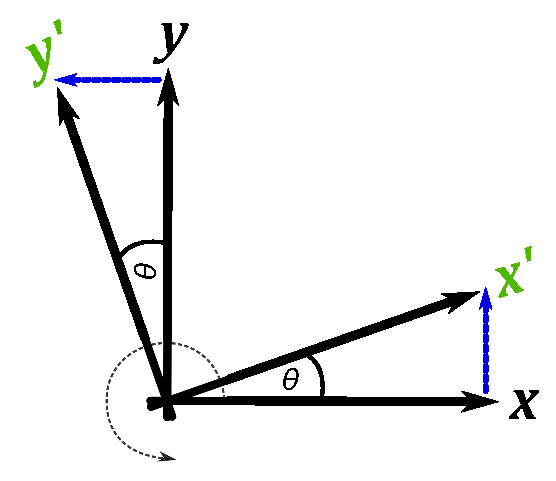
\includegraphics[scale=0.8]{inf-rot.eps}
\end{center}
  \caption{\label{fig:inf-rot}
A rotation of the coordinate axes around the $\hat z$ axis.}
\end{figure}
%
Note that this only works for infinitesimal rotation since for a finite rotation there will be contributions from multiple axes, \eg $\vec \delta x \propto \hat y - \hat x$, if you can't see this just remember the rotation matrix in 2 dimension.

How about a generic rotation axis? say we pick an arbitrary rotation axis $\vec r$ and we want to rotate a vector $\vec A$, remember that the magnitude of $\vec r$ is the amount of rotation, \ie
\nbea
\vec r = a \hat x + b \hat y + c \hat z &\longrightarrow& |\vec r| = \sqrt{a^2 + b^2 + c^2} = \epsilon
\neea

Thus the change in $\vec A$ is given by
\nbea
\vec \delta \vec A = \vec r \times \vec A & = & a (\hat x \times \vec A) + b (\hat y \times \vec A) + c (\hat z \times \vec A)
\neea

Here we see why it only works for infinitesimal rotations since rotations w.r.t different axes do not commute but they only contribute at $\epsilon^2$.

What if instead of a vector we have a scalar $A$? First we need to convert it into a vector, but how? there are many ways of doing it. If we look back to translation $A(x) \rightarrow A(x + \epsilon)$ the transformation we get is $A \rightarrow A + \epsilon \partial A$. Now, we just need to turn this into a vector, the most obvious way is $A \rightarrow A + \vec\epsilon \cdot  (\vec \nabla A)$ (note: we always need a derivative to calculate $\delta A$ thanks to taylor expansion).

Using the formula we have above 
\nbea
\vec \delta (\nabla A) = \vec r \times \nabla A & = & a (\hat x \times \nabla A) + b (\hat y \times \nabla A) + c (\hat z \times \nabla A)
\neea
however the result we have is a vector we need a scalar since $A$ was initially a scalar. The solution is just to take a dot product with $\vec x = \frac{1}{\sqrt{3}}(\hat x + \hat y + \hat z)$
\nbea
\delta A = \vec x \cdot (\vec r \times \nabla A) & = & - \vec r \cdot (\vec x \times \nabla A)
\neea
by using a triple scalar product rule, the thing here now is that I don't know how to get rid of that minus sign LOL

So for a general scalar field you'll get $\delta \phi = \vec \epsilon \cdot (\vec x \times \nabla) \phi$, sans a minus sign, where $\vec x$ is just the coordinate axes and $\vec \epsilon$ is the magnitude and axis of rotation.

Now, how does the lagrangian change? Well, the lagrangian is also a scalar quantity thus we can expect it to also change as $\delta \mathcal{L} =  \vec \epsilon \cdot (\vec x \times \nabla) \mathcal{L}$.

The goal here is to show that $\delta \mathcal{L}$ is related to the stress energy tensor {\it of translation} and for simplicity we will ignore $\vec \epsilon \cdot$ for now
\nbea
(\vec x \times \nabla) \mathcal{L} & = & \epsilon^{ijk} x_j \partial_k \mathcal{L} = \partial_\mu (\epsilon^{ijk} x_j \delta^\mu_k \mathcal{L}) \\
& = & \partial_\mu \mathcal{F}^{\mu i} \\
\rightarrow \mathcal{F}^{\mu i} & = & \epsilon^{ijk} x_j \delta^\mu_k \mathcal{L}
\neea
Since this is a symmetry the change must be a total derivative.

Now from the generic formula for energy stress tensor (under rotation)
\nbea
\widetilde T^{\mu i} & = & \frac{\delta \mathcal{L}}{\delta(\partial_\mu \phi)} \delta \phi - \mathcal{F}^{\mu i} \\
& = & \frac{\delta \mathcal{L}}{\delta(\partial_\mu \phi)} (\vec x \times \vec \nabla) \phi - \epsilon^{ijk} x_j \delta^\mu_k \mathcal{L} \\
& = & \epsilon^{ijk} x_j \left (  \frac{\delta \mathcal{L}}{\delta(\partial_\mu \phi)} \partial_k \phi - \delta^\mu_k \mathcal{L} \right ) =  \epsilon^{ijk} x_j (T^\mu_k) \\
& = & \vec x \times \vec T^\mu
\neea

Notes on energy stress tensor:
Under symmetry transformations, the lagrangian should change by a total derivative (since a symmetry should not change the physics)
\nbea
\delta\mathcal{L} & = & \partial_\mu \mathcal{F}^\mu
\neea 

However the transformation is also given by
\nbea
\delta\mathcal{L} & = & \frac{\delta \mathcal{L}}{\delta\phi}\delta \phi + \frac{\delta \mathcal{L}}{\delta(\partial_\mu \phi)} \delta(\partial_\mu \phi) \\
& = & \partial_\mu \left ( \frac{\delta \mathcal{L}}{\delta(\partial_\mu \phi)} \right ) \delta \phi + \frac{\delta \mathcal{L}}{\delta(\partial_\mu \phi)} \partial_\mu(\delta\phi) \\
\partial_\mu \mathcal{F}^\mu & = & \partial_\mu \left ( \frac{\delta \mathcal{L}}{\delta(\partial_\mu \phi)} \delta \phi \right ) \\
0 & = & \partial_\mu \left ( \frac{\delta \mathcal{L}}{\delta(\partial_\mu \phi)} \delta \phi - \mathcal{F}^\mu \right ) = \partial_\mu J^\mu \\
\rightarrow J^\mu & = & \frac{\delta \mathcal{L}}{\delta(\partial_\mu \phi)} \delta \phi - \mathcal{F}^\mu
\neea
where we have used the equation of motion on the first term going into the second line, this is actually tricky if we apply wrongly we will get something like (doing Integration by parts on the second term at the same time)
\nbea
\delta\mathcal{L} & = & \frac{\delta \mathcal{L}}{\delta\phi}\delta \phi + \frac{\delta \mathcal{L}}{\delta(\partial_\mu \phi)} \delta(\partial_\mu \phi) = \frac{\delta \mathcal{L}}{\delta\phi}\delta \phi - \partial_\mu \left ( \frac{\delta \mathcal{L}}{\delta(\partial_\mu \phi)} \right ) \delta \phi \\
& = & \partial_\mu \left ( \frac{\delta \mathcal{L}}{\delta(\partial_\mu \phi)} \right ) \delta \phi  - \partial_\mu \left ( \frac{\delta \mathcal{L}}{\delta(\partial_\mu \phi)} \right ) \delta \phi \\
& = & 0 ~~~ ???
\neea
LOL indeed but what went wrong? One, we can't really use IBP here since we are not really under an integral. However we can just use the usual trick, $u(dv) = d(uv) - (du)v$
\nbea
\frac{\delta \mathcal{L}}{\delta\phi}\delta \phi + \frac{\delta \mathcal{L}}{\delta(\partial_\mu \phi)} \delta(\partial_\mu \phi) & = & \frac{\delta \mathcal{L}}{\delta\phi}\delta \phi + \partial_\mu \left ( \frac{\delta \mathcal{L}}{\delta(\partial_\mu \phi)} \delta \phi \right ) - \partial_\mu \left ( \frac{\delta \mathcal{L}}{\delta(\partial_\mu \phi)} \right ) \delta \phi \\
& = & \left \{ \frac{\delta \mathcal{L}}{\delta\phi}\delta \phi - \partial_\mu \left ( \frac{\delta \mathcal{L}}{\delta(\partial_\mu \phi)} \right ) \delta \phi \right \} + \partial_\mu \left ( \frac{\delta \mathcal{L}}{\delta(\partial_\mu \phi)} \delta \phi \right ) \\
& = & 0 + \partial_\mu \left ( \frac{\delta \mathcal{L}}{\delta(\partial_\mu \phi)} \delta \phi \right )
\neea
again using the equations of motion for $\phi$.


-=-=-=-=-=-=-=-=-=-=-=-=-=-=-=-=-=-=-=-=-=-=-=-=-=-=-=-=-

In QFT, why does $\phi(x)$ create a particle at spacetime point $x$, \ie $\phi(x)| 0 \rangle = |x \rangle$? For simplicity we'll set $t = 0 \rightarrow \phi(x) = \phi(\vec x, 0)$. To see this take the inner product of
\nbea
\langle \vec x | \vec p \rangle & = & \langle 0 |\phi^\dagger(\vec x, 0) | \vec p \rangle \\
& = & \langle 0 | \left ( \int \frac{d^3 p'}{(2 \pi)^3 \sqrt{\omega_{p'}}} a^\dagger e^{-i\vec {p'} \vec x} +  a e^{i\vec {p'} \vec x} \right ) | \vec p \rangle \\
& = & \left ( \langle 0 | \int \frac{d^3 p'}{(2 \pi)^3 \sqrt{\omega_{p'}}} a e^{i\vec {p'} \vec x} \right ) | \vec p \rangle, ~~~ ( \langle 0 | a^\dagger ) = 0 \\
& = & \int \frac{d^3 p'}{(2 \pi)^3 \sqrt{\omega_{p'}}} e^{i\vec {p'} \vec x} ~~ \{ \langle \vec {p'} | \vec p \rangle \} \\
& = & \int \frac{d^3 p'}{(2 \pi)^3 \sqrt{\omega_{p'}}} e^{i\vec {p'} \vec x} ~~ \left \{ (2 \pi)^3 \sqrt{\omega_{p}} \delta (\vec {p'} - \vec p) \right \} \\
\langle \vec x | \vec p \rangle & = & e^{i\vec {p} \vec x}
\neea
Thus $\phi(x)$ does indeed create a particle at spacetime point $x$ :)

-=-=-=-=-=-=-=-=-=-=-=-=-=-=-=-=-=-=-=-=-=-=-=-=-=-=-=-=-

What is the explicit formula for multiple integrations of a function, \ie what is $\int\int \dots \int f(x) dx$ ? The answer is the Cauchy formula for repeated integration
\nbea
(J f)(x) & = & \int_0^x f(t) dt \\
(J^2 f)(x) & = & \int_0^x \left ( \int_0^t f(s) ds \right ) dt \\
(J^\alpha f)(x) & = & \frac{1}{(\alpha - 1)!}\int_0^x (x - t)^{\alpha-1} f(t) dt \\
& = & \frac{1}{\Gamma(\alpha)}\int_0^x (x - t)^{\alpha-1} f(t) dt
\neea
Here we have used $J$ as an integration operator and the identity $\Gamma(\alpha) = (\alpha-1)!$, and also that gamma function can take non integer arguments compared to factorials.

So how do we derive this? The most intuitive derivation I saw was using Laplace transform, some preliminary Laplace transforms that we need are

1. Laplace transform of an integral of a function, $\mathcal{L}\{\int_0^x f(t) dt\}$
\nbea
\mathcal{L}\left \{\int_0^x f(t) dt \right \} & = & \int_0^\infty e^{-sx} \left ( \int_0^x f(t) dt \right ) dx
\neea
we now use integration by parts, $u = \left ( \int_0^x f(t) dt \right ),~dv = e^{-sx} dx $ such that
\nbea
\mathcal{L}\left \{\int_0^x f(t) dt \right \} & = &  \left. \left ( \int_0^x f(t) dt \right ) \frac{e^{-sx}}{(-s)} \right |_{x = 0}^{x = \infty} - \left ( -\frac{1}{s} \right ) \int_0^\infty e^{-sx} f(x) dx \\
& = & 0 + \frac{1}{s} \int_0^\infty e^{-sx} f(x) dx \\
\mathcal{L}\left \{ (J f) (x) \right \} & = & \frac{1}{s}\mathcal{L}\left \{ f(x) \right \} 
\neea
the boundary terms are zero because $\int_0^0 f(t) = 0$ and $e^{-\infty}=0$, assuming $f(t)$ is well behaved. Generalizing to $(J^\alpha f)(x)$ we have
\nbea
\mathcal{L}\left \{ (J^\alpha f) (x) \right \} & = & \frac{1}{s^\alpha}\mathcal{L}\left \{ f(x) \right \} 
\neea

2. Laplace transform of $x^\alpha$, \ie $\mathcal{L}\{x^\alpha\}$ (all function under Laplace transform are assumed to be valid only on the positive real axis)
\nbea
\mathcal{L}\left \{x^\alpha\right \} & = & \int_0^\infty e^{-sx} x^\alpha dx
\neea
here we just need to do multiple integration by parts with $u = x^\alpha,~dv = e^{-sx} dx$
\nbea
\mathcal{L}\left \{x^\alpha\right \} & = &  \left. x^\alpha e^{-sx} \right |_{x=0}^{x=\infty} - \frac{\alpha}{(-s)}\int_0^\infty x^{\alpha-1} e^{-sx} dx \\
& = & \frac{\alpha}{s}\int_0^\infty x^{\alpha-1} e^{-sx} dx
\neea
here we can do 2 things, one use the definition of gamma function $\Gamma(\alpha) = \int_0^\infty x^{\alpha-1} e^{-x} dx$ or repeat the integration by parts again (note that the boundary terms are again zero in this case), if we repeat the IBP $\alpha-1$ more times we get
\nbea
\mathcal{L}\left \{x^\alpha\right \} & = & \frac{\alpha !}{s^\alpha}\int_0^\infty e^{-sx} dx \\
& = & \left. \frac{\alpha !}{s^\alpha} \frac{1}{(-s)} e^{-sx} \right |_{0}^{\infty} \\
& = & -\frac{\alpha !}{s^{\alpha+1}} \left ( e^{-\infty}- e^0\right ) \\
\mathcal{L}\left \{x^\alpha\right \}  & = & \frac{\alpha !}{s^{\alpha+1}}
\neea
which can be generalized to $\mathcal{L}\left \{x^\alpha\right \}  = \frac{\Gamma(\alpha+1)}{s^{\alpha+1}}$ {\it or} just by using the definition of gamma function from the beginning
\nbea
\frac{\alpha}{s}\int_0^\infty x^{\alpha-1} e^{-sx} dx & = & \frac{\alpha}{s}\int_0^\infty \left (\frac{y}{s}\right )^{\alpha-1} e^{-y} \left (\frac{dy}{s} \right), ~~~ y = sx,~ dx = \frac {dy}{s}\\
& = & \frac{\alpha}{s^{\alpha+1}}\int_0^\infty y^{\alpha-1} e^{-y} dy = \frac{\alpha \Gamma(\alpha)}{s^{\alpha+1}},~~~ \alpha \Gamma(\alpha) = \Gamma(\alpha+1)\\
\mathcal{L}\left \{x^\alpha\right \} & = & \frac{\Gamma(\alpha + 1)}{s^{\alpha+1}}
\neea
which is the same result as above.

3. The infamous convolution formula 
\nbea
\mathcal{L}\{f\}\mathcal{L}\{g\} & = & \left (\int_0^\infty e^{-sx} f(x) dx\right )\left (\int_0^\infty e^{-sy} g(y) dy\right ) \\
& = & \int_0^\infty e^{-s(x+y)}  \left ( \int_0^{\infty} f(x) g(y) dy \right ) dx, ~~~ z = x + y \\
& = & \int_0^\infty e^{-s z} \left ( \int_0^{z} f(z-y) g(y) dy \right ) dz \\
\mathcal{L}\{f\}\mathcal{L}\{g\} & = & \mathcal{L} \{ f * g\}
\neea
where $*$ denotes convolution, some explanation on $dx \rightarrow dz$, inside the brackets of $\int dy$, $x$ is constant while outside of this bracket $y$ is {\it constant} and thus $dz = dx$.
 
We are now ready to derive the formula for $(J^\alpha f)(x)$
\nbea
(J^\alpha f)(x) & = & \mathcal{L}^{-1} \{ \mathcal{L} \{J^\alpha f\} \} \\
& = & \mathcal{L}^{-1} \left \{ \frac{1}{s^\alpha} \mathcal{L} \{ f\} \right \} = \mathcal{L}^{-1} \left \{ \frac{\Gamma(\alpha)}{\Gamma(\alpha)}\frac{1}{s^\alpha} \mathcal{L} \{ f\} \right \} \\
& = & \frac{1}{\Gamma(\alpha)}\mathcal{L}^{-1} \left \{ \frac{\Gamma(\alpha)}{s^\alpha} \mathcal{L} \{ f\} \right \} \\
& = & \frac{1}{\Gamma(\alpha)} \left ( \mathcal{L}^{-1} \left \{ \frac{\Gamma(\alpha)}{s^\alpha} \right \} *  f \right ) \\
& = & \frac{1}{\Gamma(\alpha)} \left ( x^{\alpha-1} *  f \right ) \\
(J^\alpha f)(x) & = & \frac{1}{\Gamma(\alpha)} \int_0^x ( x - t )^{\alpha-1}  f(t) dt 
\neea
which is the Cauchy formula we were looking for.

-=-=-=-=-=-=-=-=-=-=-=-=-=-=-=-=-=-=-=-=-=-=-=-=-=-=-=-=-

{\bf Problem 1.1 Srednicki, Show that the Dirac matrices must be even dimensional. Hint: show that the eigenvalues of $\beta$ are all $\pm 1$, and that ${\rm Tr} \beta = 0$. To show that ${\rm Tr} \beta = 0$, consider \eg ${\rm Tr} \alpha_1^2 \beta$. Similarly, show that ${\rm Tr} \alpha_i = 0$.}

Some facts about Dirac matrices
%
\nbea
\{ \alpha^j, \alpha^k\}_{ab} = 2\delta^{jk}\delta_{ab} ~~~ \{ \alpha^j, \beta\}_{ab} = 0 ~~~ (\beta)^2_{ab} = \delta_{ab}
\neea
%
For eigenvalues of $\beta$ it follows immediately from $(\beta)^2_{ab} = \delta_{ab}$ its eigenvalues must be $\pm 1$.

For ${\rm Tr} \beta$ we start with
%
\nbea
{\rm Tr} (\alpha_1^2 \beta) & = & {\rm Tr} (\alpha_1 \beta \alpha_1), ~~\{ \alpha^j, \beta\}_{ab} = 0 \\
& = & {\rm Tr} (-\beta \alpha_1 \alpha_1) \\
{\rm Tr} (\alpha_1^2 \beta) & = & {\rm Tr} (\beta  \alpha_1 \alpha_1), ~~{\rm Tr}(AB) = {\rm Tr}(BA) \\
\rightarrow {\rm Tr} (-\beta \alpha_1 \alpha_1) & = & {\rm Tr} (\beta \alpha_1 \alpha_1) \\
{\rm Tr} (\beta \alpha_1 \alpha_1) & = & 0
\neea
%
Now from $\{ \alpha^j, \alpha^k\}_{ab} = 2\delta^{jk}\delta_{ab} \rightarrow \{ \alpha_i, \alpha_i\}_{ab} = 2 \delta_{ab}$, it means that $(\alpha^2_i)_{ab} = \delta_{ab}$ and thus ${\rm Tr} (\beta \alpha_i \alpha_i) = {\rm Tr} (\beta) = 0$.

Now since ${\rm Tr} \beta = 0$ and its eigenvalues are $\pm 1$, $\beta$ must be even dimensional.

This argument applies for ${\rm Tr} \alpha_i$ as well by reversing the roles of $\beta$ and $\alpha$, ${\rm Tr} (\beta^2 \alpha_i) = {\rm Tr} (\alpha_i) = 0$ and since $(\alpha^2_i)_{ab} = \delta_{ab} \rightarrow$ eigenvalues must be $\pm 1$, $\alpha^i$ must be even dimensional. This means that {\it all} of Dirac matrices must be even dimensional.

Now we need to show that Dirac matrices must be bigger than $2 \times 2$. I'll start with the fact that any $2 \times 2$ matrix can be written as $ a_0 1 + a_i \sigma^i$, \ie a combination of Pauli matrices and the identity matrix. If you remember some sort of group theory, the group $su(2)$ spans a three sphere and the basis vectors (lie algebra $SU(2)$) are spanned by the Pauli matrices.

The commutation relations of Pauli matrices are
%
\nbea
\{\sigma^i, \sigma^j\}_{ab} & = & 2\delta^{ij} \delta_{ab} \\
\lbrack \sigma^i, \sigma^j \rbrack & = & 2 i \varepsilon^{ijk} \sigma^{k} 
\neea
%
As we can see from their anticommutation relations, the pauli matrices can play the role of $\alpha^i$. We now need to show that there are no fourth $2\times2$ matrix to play the role of $\beta$. To do this let's construct a generic $2\times2$ matrix $A = a_0 1 + a_i \sigma^i$ and do its commutation relation with the pauli matrices and see what coefficients $(a_0, a_i)$ we need to fulfill the commutation relation $\{ \alpha^j, \beta\}_{ab} = 0$
%
\nbea
\{A, \sigma^j\} & = & \{a_0 1 + a_i \sigma^i,  \sigma^j\} \\
0 & = & \{a_0 1,  \sigma^j\}  + \{a_i \sigma^i,  \sigma^j\} \\
0 & = & 2 a_0 \sigma^j + a_i \delta^{ij} 1 \\
0 & = & 2 a_0 \sigma^j + a_j 1
\neea
%
Recall that there's only one diagonal pauli matrix, \ie if you use $\hat z$ as the main direction $\sigma_z = (+1, -1)$ which is just spin up and spin down and the other two pauli matrices will be off diagonal, if you choose any other axis the same will occur, only one will be diagonal and the other two will be off diagonal.

From $0 = 2 a_0 \sigma^j + a_j 1$, we need $\sigma^j$ to be diagonal but since $\sigma^j = (+1, -1)$ the only solution is $a_0 = 0, a_j = 0$. However the anticommutation relation $\{A, \sigma^j\} = 0$ has to be true for all values of $j = 1,2,3$ which means that $a_1 = a_2 = a_3 = 0 \rightarrow A = 0$, so the only $2\times2$ matrix that can fulfill the role of $\beta$ is the zero matrix. However, $\beta^2 = 1$, hence Dirac matrices must be at least $4\times4$.

-=-=-=-=-=-=-=-=-=-=-=-=-=-=-=-=-=-=-=-=-=-=-=-=-=-=-=-=-

{\bf Srednicki Problem 4.1 Verify eq. (4.12). Verify its limit as $m \rightarrow 0$. Eq. 4.12 is $\lbrack \varphi^+(x),\varphi^-(x') \rbrack = (m/4\pi^2 r) K_1(mr) \equiv C(r)$ where $K_1(mr)$ is a modified Bessel function of the second kind.}

The subject here is that for a transition amplitude to be Lorentz invariance, the above commutator must be zero, however it's not. Why does it have to be zero? because the transition amplitude is given by time ordered product of the fields and for spacelike separations, $x-x' > 0$, the time ordering might shuffle the order of the fields as for a spacelike separation different observers might see two events happen in different orders. Note that the metric used here is $(-+++)$. Hence the need to set $\lbrack \varphi^+(x),\varphi^-(x') \rbrack = 0$ to maintain equal transition amplitudes for all observers, $\langle \varphi(x) \varphi(y) \rangle = \langle \varphi(y) \varphi(x) \rangle$.

However, eq. 4.12 shows that $\lbrack \varphi^+(x),\varphi^-(x') \rbrack \neq 0$! Our task at hand is to derive this conclusion. First we need to choose a frame where $t-t'=0$ as suggested by the text to simplify calculation.
%
\nbea
\int \widetilde{dk} ~e^{ik(x-x')} & = & \int \frac{d^3k}{(2 \pi)^3 2 \sqrt{k^2 + m^2}} e^{(-ik_0 \Delta t + i \vec k \cdot \Delta \vec x)}, ~\Delta t = 0 \\
& = &  \int \frac{d^3k}{(2 \pi)^3 2 \sqrt{k^2 + m^2}} e^{(i\vec k \cdot \Delta \vec x)}\\
& = &  \int \frac{d^3k}{(2 \pi)^3 2 \sqrt{k^2 + m^2}} e^{i|k||r| \cos \theta}, ~ |r| = |\Delta \vec x|\\
& = &  \int \frac{k^2 dk~ d\phi~ d(\cos\theta)} {(2 \pi)^3 2 \sqrt{k^2 + m^2}} e^{i|k||r| \cos \theta}\\
& = &  \int \frac{k^2 dk~ \bcancel{2 \pi}} {(2 \pi)^{\bcancel{3}2} 2 \sqrt{k^2 + m^2}} \int^1_{-1} d(\cos\theta)~e^{i|k||r| \cos \theta}\\
& = &  \int \frac{k^2 dk} {(2 \pi)^2 2 \sqrt{k^2 + m^2}} \frac{(e^{i|k||r|} - e^{-i|k||r|})}{ikr}\\
& = &  \int \frac{k dk} {(2 \pi)^2 \bcancel{2} \sqrt{k^2 + m^2}} \frac{\bcancel{2}\bcancel{i}\sin(k r)}{\bcancel{i}r}\\
& = &  \frac{1} {(2 \pi)^2 r} \int_0^\infty dk \frac{k \sin(k r)} {\sqrt{k^2 + m^2}} 
\neea
%
We now need to massage this into a Bessel function, but first let's do a change of variable $ \rightarrow y = k/m$
%
\nbea
& = &  \frac{1} {(2 \pi)^2 r}  \int_0^\infty m ~d\left(\frac{k}{m}\right) \frac{m \left(\frac{k}{m}\right) \sin(\left(\frac{k}{m}\right) m r)} {m \sqrt{\left(\frac{k}{m}\right)^2 + 1}} \\
& = &  \frac{m} {(2 \pi)^2 r}  \int_0^\infty dy \frac{y \sin(y m r)} {\sqrt{y^2 + 1}} 
\neea
%
now, there are 2 facts we need about Bessel functions
%
\nbea
K_0(z) & = & \int_0^\infty dy \frac{\cos(zy)}{\sqrt{y^2 + 1}} \\
\frac{d}{dz} K_\nu(z) & = & \frac{\nu}{z} K_{\nu}(z) - K_{\nu+1}(z) \\
\rightarrow \frac{d}{dz} K_0(z) & = & - K_{1}(z)
\neea
%
If we do the actual derivative on $K_0$ we get
%
\nbea
\rightarrow \frac{d}{dz} K_0(z) & = & \int_0^\infty dy \frac{d}{dz} \left (\frac{\cos(zy)}{\sqrt{y^2 + 1}} \right ) \\
- K_{1}(z) & = & - \int_0^\infty dy \frac{y \sin(zy)}{\sqrt{y^2 + 1}} \\
\rightarrow \frac{m} {(2 \pi)^2 r} K_{1}(z) & = & \frac{m} {(2 \pi)^2 r} \int_0^\infty dy \frac{y \sin(zy)}{\sqrt{y^2 + 1}}, ~ z \rightarrow mr \\
\frac{m} {4 \pi^2 r} K_{1}(mr) & = & \frac{m} {(2 \pi)^2 r} \int_0^\infty dy \frac{y \sin(mr y)}{\sqrt{y^2 + 1}} \\
\frac{m} {4 \pi^2 r} K_{1}(mr) & = & \int \widetilde{dk} ~e^{ik(x-x')}
\neea
%
and that is the result that we want. How about its limit as $m \rightarrow 0$? One might be tempted to find or calculate the power series expansion of the Bessel function around $z \rightarrow 0$ but I found it extremely difficult (as I've forgotten most of the methods from my mathematical methods class) but (after looking at the problem long enough) I realized that we need not mess with Bessel functions at all.

You see $\int \widetilde{dk} ~e^{ik(x-x')}$ looks a lot like a fourier transform and setting $m \rightarrow 0$ makes it look like this
%
\nbea
& = &  \int \frac{d^3k} {(2 \pi)^3 2 \sqrt{k^2 + m^2}} e^{i \vec k \cdot \vec r}, ~m \rightarrow 0\\
& = &  \frac{1}{2 (2 \pi)^3} \int d^3k \frac{e^{i \vec k \cdot \vec r}}{|k|}
\neea
%
which looks a lot like the fourier transform of the Coulomb potential but this time it's going into the $\vec x$ domain instead of the $\vec k$ domain.

The evaluation of this integral is usually done using a regulator $e^{-\mu k}$ and we'll take the limit $\mu \rightarrow 0$ at the end.
%
\nbea
& = & \frac{1}{2 (2 \pi)^3} \int d^3k \frac{e^{-\mu k} e^{i \vec k \cdot \vec r}}{|k|} \\
& = & \frac{1}{2 (2 \pi)^3} \int k^{\bcancel{2}} dk ~ d\phi~ \frac{e^{-\mu k}}{\bcancel{k}} \int_{-1}^1 d(\cos\theta) e^{i |k| |r| \cos \theta} \\
& = & \frac{1}{2 (2 \pi)^2} \int_0^\infty \bcancel{k} dk ~ e^{-\mu k} \frac{(e^{i k r} - e^{-i k r})}{i \bcancel{k} r} \\
& = & \frac{1}{2 i r (2 \pi)^2} \int_0^\infty dk ~ e^{-\mu k} (e^{i k r} - e^{-i k r}) \\
& = & \frac{1}{2 i r (2 \pi)^2} \left \lbrack \frac{1}{(-\mu + ir)} \left. e^{(-\mu + i r)k} \right |_0^\infty - \frac{1}{(-\mu - ir)} \left. e^{(-\mu - i r)k} \right |_0^\infty \right \rbrack \\
& = & \frac{1}{2 i r (2 \pi)^2} \left \lbrack \frac{1}{(-\mu + ir)} (e^{-\infty} - e^0 ) - \frac{1}{(-\mu - ir)} (e^{-\infty} - e^0 ) \right \rbrack \\
& = & \frac{1}{2 i r (2 \pi)^2} \left \lbrack \frac{1}{(-\mu - ir)} - \frac{1}{(-\mu + ir)} \right \rbrack =  \frac{1}{2 i r (2 \pi)^2} \left \lbrack \frac{-\mu + ir + \mu + ir}{\{(-\mu)^2 - (ir)^2\}} \right \rbrack \\
& = & \frac{1}{\bcancel{2 i r} (2 \pi)^2} \frac{\bcancel{2 i r}}{\{(-\mu)^2 + r^2\}}, ~\mu \rightarrow 0 \\
& = & \frac{1}{4 \pi^2 r^2}
\neea
%
which is the result we want :) without messing with Bessel functions at all

-=-=-=-=-=-=-=-=-=-=-=-=-=-=-=-=-=-=-=-=-=-=-=-=-=-=-=-=-

How do you do the integral of $\int_{-\infty}^{\infty} dx \frac{\sin x}{x}$? The common solution is to do a contour integration, but is there another way? This was what I attempted, the answer to that question is in short no, but I sure learned a hell lot thinking about this problem.

First, there's no function whose derivative is $\frac{\sin x}{x}$ which means that the indefinite integral $\int dx \frac{\sin x}{x}$ has no solution. Contour integral was a neat technique apropos to a numerical calculation.

My original approach was inspired by green's function method. This was because the integral $\int dx \frac{\sin x}{x}$ is akeen to $\int dk \frac {e^{ikx}}{k}$ and since $\cos k$ is even, only the $\sin k$ term will survive the integration $\rightarrow \int dk \frac {i\sin (kx)}{k}$ and by taking $x \rightarrow 1$ we'll get $\int dk \frac{i \sin k}{k}$ which is what we want. The starting point is the unit step function $u(x)$
%
\nbea
\frac{d}{dx} u(x) & = & \delta(x) \\
\rightarrow ik ~ u(k) & = & 1 \\
u(k) & = & \frac{1}{ik}
\neea
%
We must take a pause here. First some trivial things, I have chosen the fourier transform pair to be $f(x) = \frac{1}{2\pi} \int dk e^{ikx} F(k)$ and $F(k) = \int dx e^{-ikx} f(x)$, \ie we put all factor of normalization $\frac{1}{2\pi}$ in the inverse transform. We can choose other normalization schemes, but the result will be the same.

The second reason to pause here is more serious. The unit step function is a peculiar function. Note that
%
\nbea
\frac{d}{dx}  \left ( u(x) + C \right ) & = & \delta(x)
\neea
%
is still true for any constant $C$. But there's a particular value of $C$ that has serious ramifications, \ie $C = -\frac{1}{2}$. Why? because
%
\nbea
\left (u(x) - \frac{1}{2} \right ) & = & \frac{1}{2} \left ( u(x) - u(-x) \right )
\neea
%
that is $\left (u(x) - \frac{1}{2} \right )$ is just the antisymmetric part of $u(x)$. Now there is a fact that we need to remember, an antisymmetric (real) function has as its fourier counterpart a purely imaginary function $\int dx e^{-ikx} f(x) = -i\int dx \sin(kx) f(x)$. We see above that $u(k) = \frac{1}{ik}$ (purely imaginary) and since $\frac{d}{dx} u(x) = \frac{d}{dx}  \left ( u(x) + C \right )$ what we were really doing was fourier transforming only the antisymmetric part of $u(x)$, \ie
%
\nbea
\frac{d}{dx}  \left ( \frac{1}{2} (u(x) - u(-x)) \right ) & = & \frac{d}{dx}  \left ( u(x) - \frac{1}{2} \right )  = \delta(x) \\
\mathcal{F}\left \{ \frac{d}{dx}  \left ( u(x) - \frac{1}{2} \right ) \right \} & = & \mathcal{F}\left \{ \delta(x) \right \} \\
ik ~\mathcal{F} \left \{ \left ( u(x) - \frac{1}{2} \right ) \right \} & = & 1 \\
ik \left ( u(k) - \frac{1}{2} (2\pi \delta(k)) \right ) & = & 1 \\
u(k) & = & \frac{1}{ik} + \pi \delta(k)
\neea
%
Note that $\mathcal{F}\left \{ \delta(x) \right \} = 1$ and $\mathcal{F}\left \{ 1 \right \} = 2\pi \delta(k)$ is affected by the normalization scheme, other schemes will produce different numerical factors. Now, what does it have to do with $\int dx \frac{\sin x}{x}$? Let's do an inverse fourier transform on the above function
%
\nbea
\mathcal{F}^{-1}\left \{ u(k) \right \} & = & \mathcal{F}^{-1}\left \{ \frac{1}{ik} + \pi \delta(k) \right \} \\
u(x) & = & \frac{1}{2\pi} \int_{-\infty}^{\infty} dk \frac{e^{ikx}}{ik} + \frac{1}{2\bcancel{\pi}} \int_{-\infty}^{\infty} dk~e^{ikx} \left ( \bcancel{\pi} \delta(k) \right ) \\
u(x) & = & \frac{1}{2\pi i} \int_{-\infty}^{\infty} dk \frac{e^{ikx}}{k} + \frac{1}{2}
\neea
%
Now we set $x \rightarrow 1, u(1) = 1$
%
\nbea
u(1) & = & \frac{1}{2\pi i} \int_{-\infty}^{\infty} dk \frac{e^{ik}}{k} + \frac{1}{2} \\
1 & = & \frac{1}{2\pi \bcancel{i}} \int_{-\infty}^{\infty} dk \frac{\bcancel{i} \sin k}{k} + \frac{1}{2} \\
\rightarrow \int_{-\infty}^{\infty} dk \frac{\sin k}{k} & = & \pi
\neea
%
In the second line we have used the fact that since $\frac{\cos k}{k}$ is an odd function, its integral is zero. And this is the origin of the factor of $\pi$. For the longest time I have wondered how this integral has anything to do with $\pi$. But wait, you might ask how in turn did the fourier transform pair acquire this factor of $\frac{1}{2\pi}$ in the first place?

The answer to that question is the gaussian integral $e^{-x^2/2}$. This gaussian function is the eigenfunction of the fourier transform. Let's see how it works
%
\nbea
\int_{-\infty}^{\infty} dx~ e^{-ikx} e^{-x^2/2} & = & \sqrt{2 \pi} ~e^{\frac{(-ik)^2}{4\left( \frac{1}{2} \right)}} \\
& = & \sqrt{2 \pi} ~e^{-k^2/2}
\neea
%
where we have used the gaussian integral formula $\int dx~e^{-ax^2 + bx + c} = \sqrt{\frac{\pi}{a}} e^{\frac{b^2}{4a} + c}$ and if we do an inverse transform we get
%
\nbea
\int_{-\infty}^{\infty} dk~ e^{ikx} \left ( \sqrt{2 \pi} ~e^{-k^2/2} \right ) & = & \sqrt{2 \pi}\sqrt{2 \pi}~ e^{\frac{(ix)^2}{4\left( \frac{1}{2} \right)}} \\
& = & 2 \pi ~e^{-x^2/2}
\neea
%
Thus
%
\nbea
\mathcal{F}^{-1} \left \{ \mathcal{F} \left \{ e^{-x^2/2}\right \} \right \} & = & 2 \pi ~e^{-x^2/2}
\neea
%
or equivalently
%
\nbea
e^{-(0)^2/2} & \stackrel{\text{\tiny ?}}{=} & \int_{-\infty}^{\infty} dk~ e^{ik(0)} \left ( \sqrt{2 \pi} ~e^{-k^2/2} \right ) \\
& = & \sqrt{2 \pi} \int_{-\infty}^{\infty} dk~e^{-k^2/2} =  \sqrt{2 \pi} \sqrt{2 \pi} \\
1 & \stackrel{\text{\tiny ?}}{=} & 2 \pi
\neea
%
this means that we need to absorb the extra factor of $2 \pi$ somehow, the usual way is to put a $\frac{1}{2\pi}$ in the inverse transform, another common way is to put a factor of $\frac{1}{\sqrt{2 \pi}}$ on both the fourier transform and its inverse. Note that my derivation of $\int \frac{\sin k}{k}$ does not depend on the normalization scheme, you might try it if you don't believe me ;)

But then again, how did the gaussian integral get a factor of $\pi$, well it's because we use a circle to compute it, remember?
%
\nbea
\int_{-\infty}^{\infty} e^{-x^2/2} & = & \sqrt {\left ( \int_{-\infty}^{\infty} e^{-x^2/2} \int_{-\infty}^{\infty} e^{-y^2/2}\right ) } \\
& = & \sqrt { \int_{-\infty}^{\infty} dx dy ~ e^{-(x^2 + y^2)/2}} \\
& = & \sqrt { \left ( \int_0^{2\pi} d\phi \right )\int_{0}^{\infty} r dr  ~ e^{-(r^2)/2}} \\
\int_{-\infty}^{\infty} e^{-x^2/2} & = & \sqrt {2 \pi}
\neea
%
And that my friend, is how you get a factor of $\pi$ in the first place :) Of course in the contour integration of $\int \frac{\sin x}{x}$ the factor of $\pi$ is due to the infinitesimal semi circle around $x=0$ but again, it's all due to a circle.

It took me two days to figure this out and I learned a lot about the step function and fourier transform in the process. It all started with a simple thought of whether or not it's possible to compute $\int \frac{\sin x}{x}$ wihout contour integration, turns out that it's not quite possible, sometimes we do need a new technique to solve an old problem and I gained a new respect for complex numbers.

%how to strike out texts
%$\msout{\mathsf{stuckout}}$

%$\cancel{5}$

%$\bcancel{5}$
-=-=-=-=-=-=-=-=-=-=-=-=-=-=-=-=-=-=-=-=-=-=-=-=-=-=-=-=-

Why do we need limits and what are they? Let's start with the infamous $\stackrel{\mbox{lim}}{_{x \to 0}}$. Without messing with $\delta$ and $\epsilon$ as in the usual formal definition of a limit, what a limit amounts to is (in the case $x \to 0^{+}$, \ie we're approaching the limit from the right) $\stackrel{\mbox{lim}}{_{~~x \to 0^+}}$ $\Rightarrow x > 0$ but $x$ is smaller than any positive real number.

Now how can that be? If it is smaller than any positive real number (and it's not negative) then it has to be zero. One way it is possible if we are dealing with infinities, something like 
% a sample tex on how to do horizontal curly braces
%z = \overbrace{
%    \underbrace{x}_\text{real} +
%    \underbrace{iy}_\text{imaginary}
%   }^\text{complex number}
%
\nbea
x = 0.\underbrace{000000 ~\dots ~ 00000}_\text{infinite \# of zeros}1
\neea
%
There are an infinite number of zeros before the digit $1$ so that it doesn't matter how small the real number you present me, I can always produce a smaller one by adding more zeros in between and it has to be infinite for this to work because $x$ is smaller than {\it any} positive real number. But this won't work since it is just zero! Remember that
%
\nbea
1 = 0.\underbrace{999999 ~\dots~ 99999}_\text{infinite \# of 9's}
\neea
%
Thus limits are a (more severe?) manifestation of infinities. The real question is: why do we need it? The more obvious reason is in the calculation of a slope. To calculate a slope you need at least two points, say $(x_1, y_1)$ and $(x_2, y_2)$ and the slope is
%
\nbea
\frac{\Delta y}{\Delta x} & = & \frac{(y_2 -y_1)}{(x_2 - x_1)}
\neea
%
but then whose slope is it? Is it the slope at $(x_1, y_1)$ or at $(x_2, y_2)$? because slopes at different points are usually different. What we want is to calculate the slope at {\it one} point but we need two points to calculate it. How do we solve this conundrum? The answer is of course limits! If we take the limit $\Delta x = (x_2 - x_1) \to 0^+$ we are practically using two distinct points located at the `same' place because $x_2$ is {\it not} $x_1$ and yet it is closer to $x_1$ than any other points.

In closing, in the words of my high school math teacher, ``limits bring into existence things that don't exist'' and I believe that what real numbers do. And that might be the {\it real} reason behind its difficulties, real numbers were supposed to address the problem of continuum in mathematics although physical continuum may not actually exist, maybe ``what God has not created we shouldn't bring about'' :)

-=-=-=-=-=-=-=-=-=-=-=-=-=-=-=-=-=-=-=-=-=-=-=-=-=-=-=-=-
%
\begin{figure}
\begin{center}
  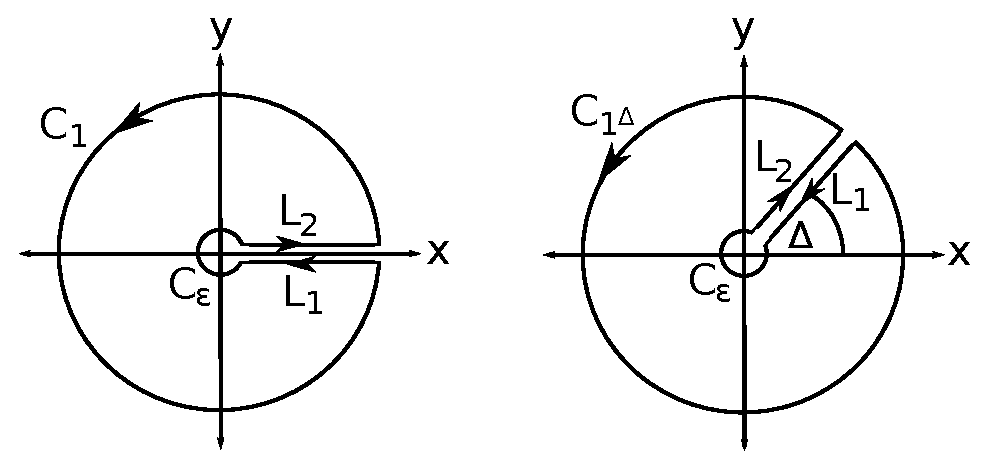
\includegraphics[scale=0.8]{branch-cut-plots/sq-root-cut.eps}
\end{center}
  \caption{\label{fig:sq-root-cut}
A choice of contour that includes a cut.}
\end{figure}
%

Branch cuts, what are they for? and how do we use them? For an illustration see Fig.~\ref{fig:sq-root-cut}. What we want to do here is to calculate $\oint_{C} \sqrt{z} dz$ along a unit circle around the origin. The tricky thing here is that $1 = e^{i0} = e^{i2\pi}$ but $\sqrt{1} \rightarrow e^{i0/2} \neq e^{i\pi}$! So we need to provide a cut such that the contour doesn't go full circle. First we will calculate $\oint_{C} \sqrt{z} dz$ using the contour shown in Fig.~\ref{fig:sq-root-cut} (left).
%
\nbea
\oint_{C} \sqrt{z} dz & = & \oint_{C_1} \sqrt{z} dz + \int_{L_1} \sqrt{z} dz + \oint_{C_\varepsilon} \sqrt{z} dz + \int_{L_2} \sqrt{z} dz \\
\rightarrow \oint_{C} \sqrt{z} dz & = & 0, ~~{\rm no~pole~inside~the~contour} \\
\rightarrow \oint_{C_1} \sqrt{z} dz & = & \int_{\varepsilon}^{2\pi - \varepsilon} \sqrt{1 e^{i\theta}} d\theta = \int_{0}^{2\pi} \sqrt{e^{i\theta}} d\theta = \oint_{C} \sqrt{z} dz \\ 
\rightarrow \int_{L_1} \sqrt{z} dz & = & \int_{1}^{\varepsilon} \sqrt{x e^{(2\pi - \varepsilon) i}} dx = \int_{1}^{0} \sqrt{x} e^{\pi i} dx = \int_{0}^{1} \sqrt{x}~ dx \\
\rightarrow \oint_{C_\varepsilon} \sqrt{z} dz & = & \int_{2\pi - \varepsilon}^{\varepsilon} \sqrt{\varepsilon e^{i \theta}} d\theta = 0 ~{\rm as}~\varepsilon \to 0 \\
\rightarrow \int_{L_2} \sqrt{z} dz & = & \int^{1}_{\varepsilon} \sqrt{x e^{\varepsilon i}} dx = \int^{1}_{0} \sqrt{x} ~dx 
\neea
%
and we take the limit of $\varepsilon \to 0$. Thus we have, after rearranging
%
\nbea
\oint_{C} \sqrt{z} dz & = & \oint_{C_1} \sqrt{z} dz + \int_{L_1} \sqrt{z} dz + \oint_{C_\varepsilon} \sqrt{z} dz + \int_{L_2} \sqrt{z} dz \\
\rightarrow 0 & = & \oint_{C} \sqrt{z} dz + \int_{0}^{1} \sqrt{x}~ dx + 0 + \int_{0}^{1} \sqrt{x}~ dx \\
\oint_{C} \sqrt{z} dz & = & - \int_{0}^{1} \sqrt{x}~ dx - \int_{0}^{1} \sqrt{x}~ dx \\
& = & -\frac{4}{3}
\neea
%
but what happens if we choose a cut that doesn't lie on the $x$ axis? say the cut is at an angle $\Delta$? as shown in Fig.~\ref{fig:sq-root-cut} (right), note that we want $L_1$ and $L_2$ to differ by $2\pi$ otherwise there's no point in introducing a cut, here $L_2$ is at angle $\Delta$ and $L_1$ is at angle $\Delta + 2\pi$
%
\nbea
\oint_{C^\Delta} \sqrt{z} dz & = & \oint_{C_{1^\Delta}} \sqrt{z} dz + \int_{L_{1^\Delta}} \sqrt{z} dz + \oint_{C_{\varepsilon^\Delta}} \sqrt{z} dz + \int_{L_{2^\Delta}} \sqrt{z} dz \\
\rightarrow \oint_{C^\Delta} \sqrt{z} dz & = & 0, ~~{\rm no~pole~inside~the~contour} \\
\rightarrow \oint_{C_{1^\Delta}} \sqrt{z} dz & = & \int_{\Delta + \varepsilon}^{\Delta + 2\pi - \varepsilon} \sqrt{1 e^{i\theta}} d\theta = \int_{\Delta}^{\Delta + 2\pi} \sqrt{e^{i\theta}} d\theta = \oint_{C^\Delta} \sqrt{z} dz \\ 
\rightarrow \int_{L_{1^\Delta}} \sqrt{z} dz & = & \int_{1}^{\varepsilon} \sqrt{r e^{(\Delta + 2\pi - \varepsilon) i}} dr = \int_{1}^{0} \sqrt{r} e^{i\Delta/2}e^{\pi i} dr = e^{i\Delta/2} \int_{0}^{1} \sqrt{r}~ dr \\
\rightarrow \oint_{C_{\varepsilon^\Delta}} \sqrt{z} dz & = & \int_{\Delta+2\pi - \varepsilon}^{\Delta+\varepsilon} \sqrt{\varepsilon e^{i \theta}} d\theta = 0 ~{\rm as}~\varepsilon \to 0 \\
\rightarrow \int_{L_{2^\Delta}} \sqrt{z} dz & = & \int^{1}_{\varepsilon} \sqrt{r e^{(\Delta+\varepsilon) i}} dr = e^{i\Delta/2} \int^{1}_{0} \sqrt{r} ~dr 
\neea
%
Now we have
%
\nbea
\oint_{C^\Delta} \sqrt{z} dz & = & \oint_{C_{1^\Delta}} \sqrt{z} dz + \int_{L_{1^\Delta}} \sqrt{z} dz + \oint_{C_{\varepsilon^\Delta}} \sqrt{z} dz + \int_{L_{2^\Delta}} \sqrt{z} dz \\
0 & = & \oint_{C^\Delta} \sqrt{z} dz + e^{i\Delta/2} \int_{0}^{1} \sqrt{r}~ dr + 0 + e^{i\Delta/2} \int^{1}_{0} \sqrt{r} ~dr \\
\oint_{C^\Delta} \sqrt{z} dz & = & -2 e^{i\Delta/2} \int_{0}^{1} \sqrt{r}~ dr \\
& = & e^{i\Delta/2} \left( -\frac{4}{3} \right )
\neea
%
So apparently we get a different result for different contours, but if we take a closer look
%
\nbea
\oint_{C^\Delta} \sqrt{z} dz & = & \int_{\Delta}^{\Delta + 2\pi} \sqrt{1 e^{i\theta}} d\theta \\
{\rm Let}~ \omega = \theta - \Delta & \rightarrow & d\omega = d\theta, ~ \int_{\Delta}^{\Delta + 2\pi} d\theta = \int_{0}^{2\pi} d\omega \\
\rightarrow \oint_{C^\Delta} \sqrt{z} dz & = & \int_{0}^{2\pi} \sqrt{1 e^{i(\omega + \Delta)}} d\omega \\
& = &  e^{i\Delta/2} \int_{0}^{2\pi} \sqrt{1 e^{i\omega}} d\omega \\
\oint_{C^\Delta} \sqrt{z} dz & = & e^{i\Delta/2} \oint_{C} \sqrt{z} dz
\neea
%
so indeed
%
\nbea
\oint_{C^\Delta} \sqrt{z} dz = e^{i\Delta/2} \oint_{C} \sqrt{z} dz & = & e^{i\Delta/2} \left( -\frac{4}{3} \right )\\
\rightarrow  \oint_{C} \sqrt{z} dz & = & -\frac{4}{3}
\neea
%
Thus rotating the branch cut (by an angle $\Delta$) does indeed rotate the original integral $\oint_{C} \sqrt{z} dz$ into $e^{i\Delta/2} \oint_{C} \sqrt{z} dz$, so we need to be careful.

A side note, how do we specify the contour if the circle is not at the origin but say is at $z_0$? Well, we can just parametrize the circle as $z = z_0 + r e^{i\theta}$ (remember that additions in the complex plane are vectorial operations), thus a contour integral of $z$ around a point $z_0$ is simply given by
%
\nbea
\oint z~dz \rightarrow \int_{0}^{2\pi} (z_0 + r e^{i\theta}) d\theta
\neea
%
%
\begin{figure}
\begin{center}
  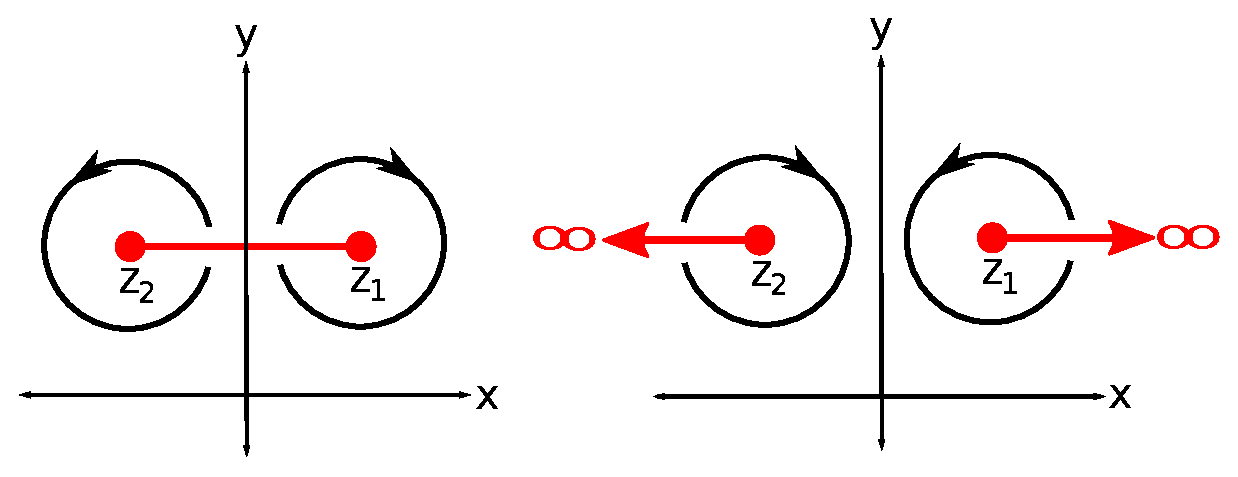
\includegraphics[scale=0.7]{branch-cut-plots/2-root-cut.eps}
\end{center}
  \caption{\label{fig:2-root-cut}
Different choices of contours that include a cut with 2 roots.}
\end{figure}
%
Going back to branch cuts, what if we have more than one root, \eg $\sqrt{(z-z_1)(z-z_2)}$? see Fig.~\ref{fig:2-root-cut}. Then there are two choices, we can put the cut between the roots as shown in Fig.~\ref{fig:2-root-cut} (left) or we can put the cuts starting from the roots to infinity as shown in Fig.~\ref{fig:2-root-cut} (right), the point here is to prevent a full circle around each root.

-=-=-=-=-=-=-=-=-=-=-=-=-=-=-=-=-=-=-=-=-=-=-=-=-=-=-=-=-

Throwback Tuesday! (today is Tuesday Oct 13 2015) High school favorite, how do we compute $\sin(18^\circ)$ without approximation and without a calculator? Well, start with $\sin(18^\circ) = \sin(90^\circ/5)$, since we know that $\sin(90^\circ) = 1$. However, our real starting point is actually $\cos(90^\circ/5)$ because $\cos(90^\circ) = 0$ and the end goal here is to transform $\sin(18^\circ)$ into solving a polynomial and it's easier to find the zeros of a polynomial if there's no constant.

First we need the formula for $\cos(5x)$. The easiest way to do this is to use Euler's formula
%
\nbea
e^{i5x} & = & \left ( e^{ix} \right ) ^5 \\
\rightarrow \cos(5x) + i \sin(5x) & = & \left ( \cos(x) + i \sin(x)\right )^5
\neea
%
In case you forget how to expand a polynomial, here's the Pascal's triangle
%
\nbea
& 1 & \\
1~~~ & 2 &~~~ 1 \\
1~~~ 3~ & &~ 3~~~ 1 \\
1~~~ 4~~~ & 6 &~~~ 4~~~ 1 \\
1~~~ 5~~~ 10 & & 10~~~ 5~~~ 1
\neea
%
the expansion is then
%
\nbea
\left ( \cos(x) + i \sin(x)\right )^5 & = & \cos^5(x) + 5 \cos^4(x)i\sin(x) + 10 \cos^3(x)i^2\sin^2(x) + \\
&& 10 \cos^2(x)i^3\sin^3(x) + 5 \cos(x)i^4\sin^4(x) + i^5\sin^5(x) \\
\rightarrow \cos(5x) & = & {\text {Re}} \left \{ \left ( \cos(x) + i \sin(x)\right )^5 \right \} \\
& = & \cos^5(x) - 10 \cos^3(x)\sin^2(x) + 5 \cos(x)\sin^4(x) \\
\rightarrow \sin(5x) & = & {\text {Im}} \left \{ \left ( \cos(x) + i \sin(x)\right )^5 \right \} \\
& = & 5 \cos^4(x)\sin(x) - 10 \cos^2(x)\sin^3(x) + \sin^5(x)
\neea
%
simplifying 
%
\nbea
\cos(5x) & = & \cos^5(x) - 10 \cos^3(x)\sin^2(x) + 5 \cos(x)\sin^4(x) \\
& = & \cos^5(x) - 10 \cos^3(x)(1 - \cos^2(x)) + 5 \cos(x)( 1 - \cos^2(x))^2 \\
& = & \cos^5(x) - 10 \cos^3(x) + 10 \cos^5(x) + 5 \cos(x)( 1 -2\cos^2(x) + \cos^4(x)) \\
& = & 11\cos^5(x) - 10 \cos^3(x) + 5 \cos(x) - 10\cos^3(x) + 5 \cos^5(x) \\
\cos(5x) & = & 16\cos^5(x) - 20 \cos^3(x) + 5 \cos(x)
\neea
%
while for $\sin$
%
\nbea
\sin(5x) & = & 5 \cos^4(x)\sin(x) - 10 \cos^2(x)\sin^3(x) + \sin^5(x) \\
& = & 5 (1 - \sin^2(x))^2 \sin(x) - 10 (1 - \sin^2(x))\sin^3(x) + \sin^5(x) \\
& = & 5 (1 - 2\sin^2(x) + \sin^4(x)) \sin(x) - 10 \sin^3(x) + 10 \sin^5(x) + \sin^5(x) \\
& = & 5 \sin(x) - 10\sin^3(x) + 5 \sin^5(x) - 10 \sin^3(x) + 11 \sin^5(x) \\
\sin(5x) & = & 16 \sin^5(x) - 20\sin^3(x) + 5 \sin(x)
\neea
%
We can of course derive the above result using the usual formulae, for example
%
\nbea
\sin(5x) & = & \sin(2x + 3x) \\
& = & \sin(2x)\cos(3x) + \cos(2x)\sin(3x) \\
\sin(2x) & = & 2\sin(x)\cos(x) \\
\cos(3x) & = & \cos(x + 2x) = \cos(x)\cos(2x) - \sin(x)\sin(2x) \\
\cos(2x) & = & \cos^2(x) - \sin^2(x) = 1 - 2\sin^2(x) \\
\sin(3x) & = & \sin(x + 2x) = \sin(x)\cos(2x) + \cos(x)\sin(2x)
\neea
%
and working out the algebra, the result will be the same. Now we see as to why starting out with $\sin(18^\circ) = \sin(90^\circ/5)$ doesn't work well
%
\nbea
 \sin(5 \times 18^\circ) = 1 & = & 16 \sin^5(18^\circ) - 20\sin^3(18^\circ) + 5 \sin(18^\circ) \\
1 & = & 16 \sin^5(18^\circ) - 20\sin^3(18^\circ) + 5 \sin(18^\circ)
\neea
%
the LHS is not zero, while starting with $\cos(18^\circ) = \cos(90^\circ/5)$ does work
%
\nbea
 \cos(5 \times 18^\circ) = 0 & = & 16 \cos^5(18^\circ) - 20\cos^3(18^\circ) + 5 \cos(18^\circ) \\
0 & = & \cos(18^\circ) (16\cos^4(18^\circ)  - 20\cos^2(18^\circ) + 5), ~~ {\rm Let~} x = \cos^2(18^\circ) \\
0 & = & 16x^2 - 20x + 5  \\
x & = & \frac{20 \pm \sqrt{400 - 320} }{32} = \frac{20 \pm 4\sqrt{5} }{32}
\neea
%
we just need to take the $+$ of the $\pm$ since $\cos$ of small angles are closer to one. The result we want is then given by
%
\nbea
\sin(18^\circ) & = & \sqrt{\sin^2(18^\circ)} = \sqrt{1- \cos^2(18^\circ)} = \sqrt{1 - x} \\
& = &\sqrt{ 1 - \frac{20 + 4\sqrt{5} }{32}} \\
\sin(18^\circ) & = & \sqrt{ \frac{3 - \sqrt{5} }{8} }
\neea
%
but wait, how do you calculate the square root by hand? The problem states that we should calculate it without a calculator. 

To calculate square roots by hand we use the ubiquitous formula $(a + b)^2 = a^2 + 2ab + b^2$ and do it iteratively. Say we want to find the root of a number, \eg $\sqrt{C}$, first we do a rough approximation $C_1^2 < C$ and then we find the next factor $C_2$ through
%
\nbea
C & = & (C_1 + C_2)^2 = C_1^2 + 2C_1C_2 + C_2^2 \\
(C - C_1^2) & = & (2C_1 + C_2)C_2
\neea
%
finding the largest $C_2$ such that $(2C_1 + C_2)C_2 < (C - C_1^2)$. Once we find $C_2$ we repeat the process
%
\nbea
C & = & (\{C_1 + C_2\} + C_3)^2 = \{C_1 + C_2\}^2 + 2\{C_1 + C_2\}C_3 + C_3^2 \\
(C - \{C_1 + C_2\}^2) & = & (2\{C_1 + C_2\} + C_3)C_3
\neea
%
by finding the largest $C_3$ such that $(2\{C_1 + C_2\} + C_3)C_3 < (C - \{C_1 + C_2\}^2)$. In other words
%
\nbea
C_1 & \rightarrow & {\rm largest~number~such~that~}C_1^2 < C\\
C_n & \rightarrow & {\rm largest~number~such~that~}\left ( 2\left ( \sum_{i=1}^{n-1} C_i \right ) + C_n \right ) C_n < \left ( C - \left ( \sum_{i=1}^{n-1} C_i \right )^2 \right ) \\
\rightarrow \sqrt{C} & = & \sum_{i=1}^{\infty} C_i
\neea
%
You can stop anytime you want, depending on the accuracy you need. The above prescription is correct but we want to make it more systematic by dividing the number into `hundreds', partitioning it into 2-digit groupings (hundreds because our digits run from $0$ to $9$ which translate to $0$ to $<100$). Let's see how it works with a concrete example

{\renewcommand{\arraystretch}{0.2} %<- modify value to suit your needs
\begin{tabular}{r l}
 & ~~~~2~~3~~8.~~~3~ ~0~~4~~4 \\
 & $\sqrt{~5~67~89.~01~20~00~00}$ \\
 $2 \times 2 =$ & ~~~~4\\
 & ~~~--------------------------- - \\
 & ~~~~1~67 \\
 $((2) (10) (2) + 3) \times 3= $ & ~~~~1~29\\
 & ~~~--------------------------- - \\
 &~~~~~~38~89 \\
 $((2) (10) (23) + 8) \times 8= $ & ~~~~~~37~44\\
  & ~~~--------------------------- - \\
 & ~~~~~~~~1~45~01\\
 $((2) (10) (238) + 3) \times 3= $ & ~~~~~~~~1~42~89\\
 & ~~~--------------------------- - \\
 & ~~~~~~~~~~~~2~12~20\\
 $((2)(10)(2383) + 0) \times 0= $ & ~~~~~~~~~~~~0~00~00\\
 & ~~~--------------------------- - \\
 &~~~~~~~~~~~~2~12~20~00\\
 $((2)(10)(23830) + 4) \times 4= $ &~~~~~~~~~~~~1~90~64~16\\
 & ~~~--------------------------- - \\
 &~~~~~~~~~~~~~~~21~55~84~00\\
 $((2)(10)(238304) + 4) \times 4= $ &~~~~~~~~~~~~~~~19~06~43~36\\\\\\
\end{tabular}
}

Thus $\sqrt{56789.012} = 238.3044 \dots$

What we need to take note above is that $C_1$ takes care only the first digit, this makes it a lot easier to start the procedure, rather than trying to figure out 238 from the start.

In the second iteration, we multiply $C_1$ by 10 and at the same time `multiplying' the target by 100 by including the next 2 digits as
%
\nbea
100C & = & 100(C_1 + C_2)^2 = 100 C_1^2 + 200C_1C_2 + 100 C_2^2 \\
100(C - C_1^2) & = & (2 (10) C_1 + C_2) C_2
\neea
%
Another important point is that $C_5=0$! Zero is apparently permitted. I actually learned this method when I was 10 but didn't understand the reasoning behind it.

Another way of computing square roots is using taylor expansion
%
\nbea
\sqrt{1 + x} & = & 1 + \frac{1}{2} x + \sum^{\infty}_{n=1} \frac{(-1)^n (2n-1)!!}{2^n} x^{n+1}
\neea
%
for example
%
\nbea
\sqrt{101} = 10\sqrt{1 + 0.01} & = & 10 \left (1 + \frac{1}{2} (0.01) - \frac{1}{2} (0.01)^{2} + \frac{(1) (3)}{2^2} (0.01)^{3} + \dots \right )
\neea
%
but the convergence might be slow due to the alternating signs in the series. One important note here is that although the previous method looks a lot like the usual division algorithm, they are extremely different. In the case of roots, you need to keep using the previous results to compute the next one, not so with divisions, this is because divisions are linear while roots are not.

-=-=-=-=-=-=-=-=-=-=-=-=-=-=-=-=-=-=-=-=-=-=-=-=-=-=-=-=-

Why does a number that is a multiple of 9 have digits tham sum up to be a multiple of 9? \eg
%
\nbea
3 \times 9 = 27 & \rightarrow & 2 + 7 = 9 \\
13 \times 9 = 117 & \rightarrow & 1 + 1 + 7 = 9 \\
5555 \times 9 = 49995 & \rightarrow & 4 + 9 + 9 + 9 + 5 = 36 = 4 \times 9
\neea
%
First of all, any number can be written as
%
\nbea
a_Na_{N-1}a_{N-2}\dots a_2a_1a_0 & = & \sum_{i = 0}^{N} a_i 10^i, ~~a_i \in \{0,1,2,3,4,5,6,7,8,9\}
\neea
%
\eg 10937 $\to a_4 = 1, a_3 = 0, a_2 = 9, a_1 = 3, a_0 = 7$, now say we have a number that is a multiple of 9, $b = 9 n$, with $n$ a positive integer
%
\nbea
b = 9 n & = & \sum_{i = 0}^{N} a_i 10^i \\
\sum_{i = 0}^{N} a_i 10^i & = & \sum_{i = 1}^{N} a_i (10^i - 1) + \sum_{i = 0}^{N} a_i
\neea
%
but we can rewrite
%
\nbea
\left (10^i - 1 \right ) & = & \sum_{j = 0}^{i-1} 9(10)^j = 9\sum_{j = 0}^{i-1} (10)^j \\
\rightarrow \sum_{i = 0}^{N} a_i 10^i & = & \sum_{i = 1}^{N} a_i \left (9 \sum_{j = 0}^{i-1} (10)^j \right ) + \sum_{i = 0}^{N} a_i \\
b = 9n & = & 9 \left ( \sum_{i = 1}^{N} a_i \left ( \sum_{j = 0}^{i-1} (10)^j \right ) \right ) + \sum_{i = 0}^{N} a_i \\
9 n - 9 \left ( \sum_{i = 1}^{N} a_i \left ( \sum_{j = 0}^{i-1} (10)^j \right ) \right ) & = & \sum_{i = 0}^{N} a_i \\
\neea
%
Thus the sum of the digits $\sum_{i = 0}^{N} a_i = 9m$ is a multiple of nine, \eg 41076 = $9 \times 4654$
%
\nbea
9 \times 4654 = 41076 & = & 4 \times 10000 + 1 \times 1000 + 0 \times 100 + 7 \times 10 + 6 \\
& = & (4 \times (10000-1) + 1 \times (1000-1) + 0 \times (100-1) + 7 \times (10-1)) + \\
&&  ( 4 + 1 + 0 + 7 + 6) \\
& = & (4 \times 9999 + 1 \times 999 + 0 \times 99 + 7 \times 9) + ( 4 + 1 + 0 + 7 + 6) \\
9 \times 4654 & = & 9 \times (4 \times 1111 + 1 \times 111 + 0 \times 11 + 7 \times 1) + ( 4 + 1 + 0 + 7 + 6)
\neea
%
Hence $ ( 4 + 1 + 0 + 7 + 6)$ must be a multiple of 9.

Note that the above argument is also valid for multiples of 3, \ie digits of a number that is a multiple of 3 sum up to a multiple of 3.

-=-=-=-=-=-=-=-=-=-=-=-=-=-=-=-=-=-=-=-=-=-=-=-=-=-=-=-=-

%
\begin{figure}
\begin{center}
  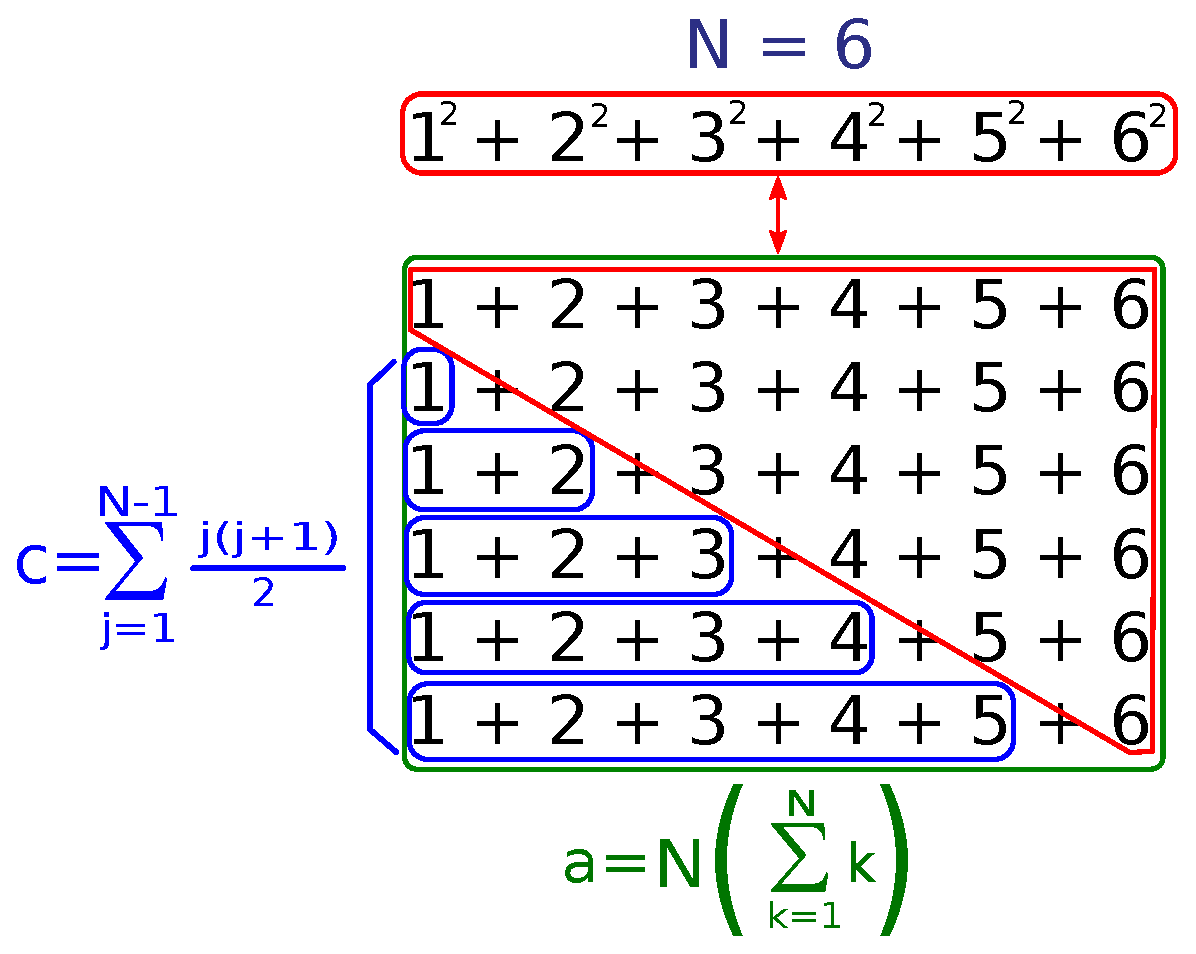
\includegraphics[scale=0.45]{n-squared-plots/n_squared_sum_box_1.eps}
\end{center}
  \caption{\label{fig:sum-sq-1}
An illustration on how to calculate sum of squares.}
\end{figure}
%
What is the explicit formula for $\sum_{i=1}^{N} i^2$? I saw this on the bus on my way to work a long time ago, took me a day to finally figure it out. You can say that we can use induction to prove the formula however, induction only allows you to prove what you already know {\it not} to derive the formula itself in the first place! {\it inductio no ex nihilo} :)

The easiest way to derive the formula for $\sum_{i=1}^{N} i^2$ is to actually draw it, see Fig.~\ref{fig:sum-sq-1}. The series we want to sum is shown in the top red box, \ie $\sum_{i=1}^{N=6} i^2 = 1^2 + 2^2 + 3^2 + 4^2 + 5^2 + 6^2$.

This sum $\sum_{i=1}^{N=6} i^2$ is also represented by the upper red triangle in Fig.~\ref{fig:sum-sq-1} because that is the definition of squares, \eg $2^2 = 2 + 2,~3^2 = 3 + 3 + 3$. However, Fig.~\ref{fig:sum-sq-1} also shows how we can calculate this upper red triangle, it is nothing but the sum in the green box $a$ minus the sum in the lower blue triangle $c$.

The sum in the green box is given by $a = 6 \times (1 + 2 + 3 + 4 + 5 +6) = N\sum_{k=1}^{N=6} k$, the lower blue triangle is given by $c= \sum^{N-1}_{j=1} \sum_{m=1}^{j} m = \sum^{N-1}_{j=1} j(j+1)/2$, where we have used the famous gauss formula for $\sum_{m=1}^{N} m = N(N+1)/2$.

The sum $\sum_{i=1}^{N} i^2$ is then given by
%
\nbea
\sum_{i=1}^{N} i^2 & = & a - c \\
& = & \left ( N\sum_{k=1}^{N} k \right ) - \left ( \sum^{N-1}_{j=1} \frac{j(j+1)}{2} \right ) \\
& = & \left ( N \frac{N(N+1)}{2}\right ) - \left ( \frac{1}{2} \sum^{N-1}_{j=1} j^2 + \frac{1}{2} \sum^{N-1}_{j=1} j \right ) \\
\sum_{i=1}^{N} i^2 & = & \left ( N \frac{N(N+1)}{2}\right ) - \left ( \left \{ \frac{1}{2} \sum^{N}_{j=1} j^2 - \frac{1}{2} N^2 \right \} + \frac{1}{2} \sum^{N-1}_{j=1} j \right ) \\
\sum_{i=1}^{N} i^2 +  \frac{1}{2} \sum^{N}_{j=1} j^2 & = & \left ( \frac{N^3 + N^2}{2}\right ) - \left ( - \frac{1}{2} N^2 + \frac{1}{2} \frac{(N-1)N}{2} \right ) \\
& = & \frac{N^3 + N^2}{2} + \frac{1}{2} N^2 -  \frac{(N-1)N}{4} \\
\frac{3}{2} \sum^{N}_{i=1} i^2 & = &  \frac{2N^3 + 2N^2 + 2N^2 - N^2 + N}{4} \\
& = & \frac{2N^3 + 3N^2 + N}{4} = \frac{N(N+1)(2N+1)}{4} \\
\rightarrow \sum^{N}_{i=1} i^2 & = & \frac{N(N+1)(2N+1)}{6}
\neea
%
And that is the formula we are after!

Bonus !!!

We can use the above result to calculate $c$ explicitly in terms of $N$
%
\nbea
c & \equiv & \sum^{N}_{j=1} \frac{j(j+1)}{2} = \frac{1}{2} \sum^{N}_{j=1} j^2 + \frac{1}{2} \sum^{N}_{j=1} j \\
& = & \frac{1}{2} \frac{2N^3 + 3N^2 + N}{6} + \frac{1}{2}\frac{N^2 + N}{2} \\
& = & \frac{2N^3 + 6N^2 + 4N}{12} = \frac{N^3 + 3N^2 + 2N}{6} \\
\sum^{N}_{j=1} \frac{j(j+1)}{2} & = & \frac{N^3 + 3N^2 + 2N}{6}
\neea
%
Now, we can use this result to get something interesting. Note that the blue lower triangle $c$ in Fig.~\ref{fig:sum-sq-1} can be seen as a sum in the vertical direction, \ie
%
\nbea
c & = & 1(5) + 2(4) + 3(3) + 4(2) + 5(1) \\
& = & 1(5 - 0) + 2(5 - 1) + 3(5 - 2) + 4(5 - 3) + 5(5 - 4) \\
& = & 5 (1 + 2 + 3 + 4 + 5) - (2(1) + 3(3) + 4(2) + 5(1)) \\
\frac{N^3 + 3N^2 + 2N}{6} & = & \left ( N\sum_{i=1}^{N} i \right ) - \sum_{i=2}^{N} i(i-1), ~~N=5
\neea
%
where in the last line we have used the explicit formula for $c$. Switching sides and generalizing to any $N$
%
\nbea
\sum_{i=2}^{N} i(i-1) & = & \left ( N\sum_{i=1}^{N} i \right ) - \frac{N^3 + 3N^2 + 2N}{6} \\
& = & \frac{N^3 + N^2}{2} - \frac{N^3 + 3N^2 + 2N}{6} \\
& = & \frac{3N^3 + 3N^2 - N^3 - 3N^2 - 2N}{6} \\
& = & \frac{2N^3 - 2N}{6} \\
\sum_{i=2}^{N} i(i-1) & = & \frac{N^3 - N}{3}
\neea
%
We can now in turn use this result to calculate $1 + 2(1) + 3(2) + 4(3) + \dots + N(N-1)$, \ie
%
\nbea
1 + \sum_{i=2}^{N} i(i-1) = 1 + \sum_{i=2}^{N} \frac{i!}{(i-2)!} = \frac{N^3 - N}{3} + 1
\neea
%
Looking back at how we calculated $\sum_{i=1}^{N} i^2$ using Fig.~\ref{fig:sum-sq-1}, we can easily generalize it to calculate $\sum_{i=1}^{N} i^k, k > 2$, see Fig.~\ref{fig:sum-sq-2}. To simplify things let's designate $f_k(N) \equiv \sum_{i=1}^{N} i^k$ as the sum of $k$-th powers.
%
\begin{figure}
\begin{center}
  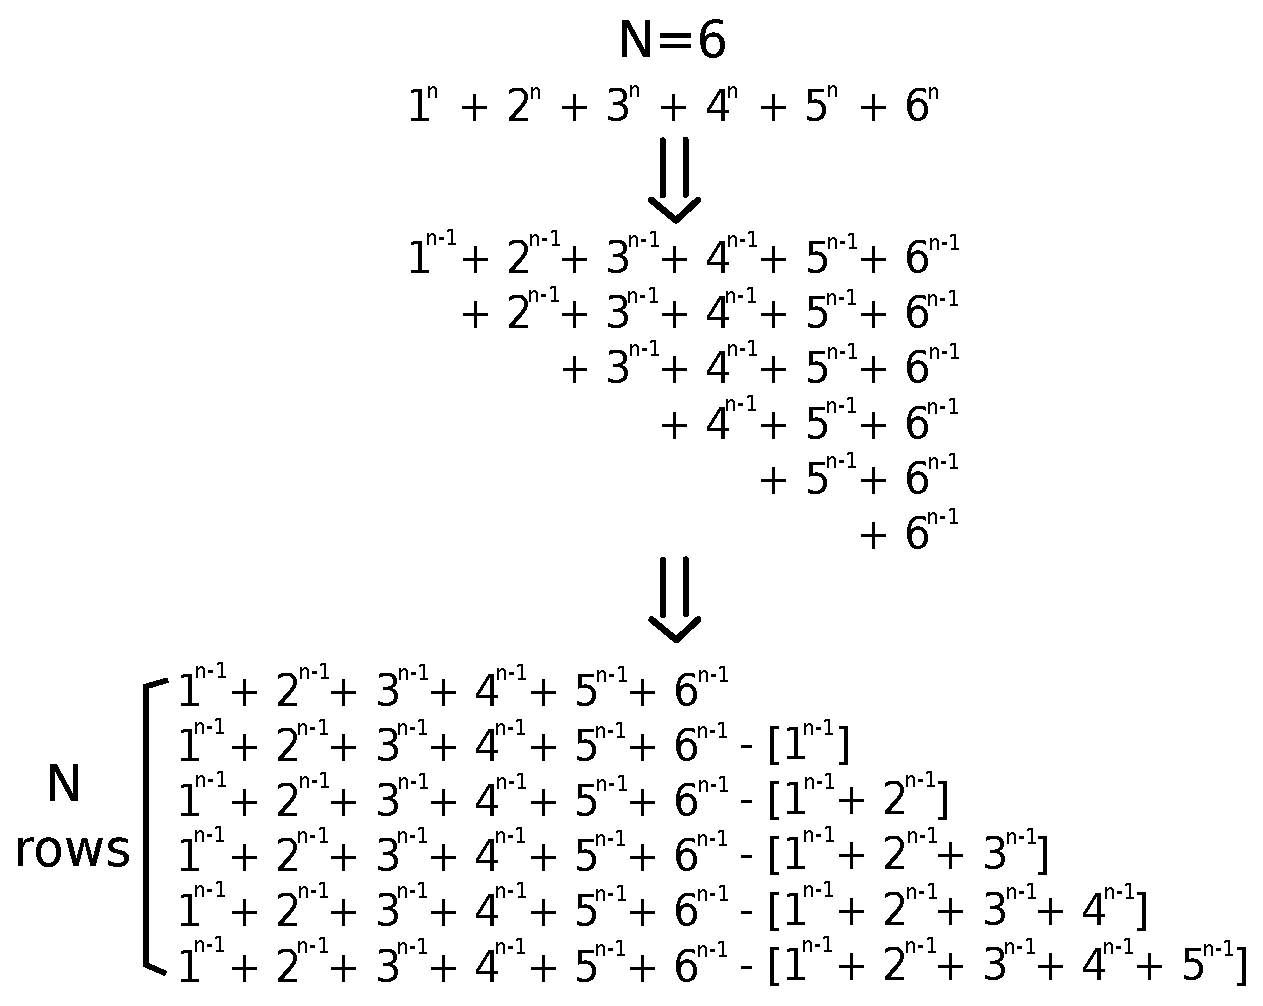
\includegraphics[scale=0.55]{n-squared-plots/n_squared_sum_box_2.eps}
\end{center}
  \caption{\label{fig:sum-sq-2}
An illustration on how to calculate sum of $n$-th powers.}
\end{figure}
%

From Fig.~\ref{fig:sum-sq-2} it's immediately apparent that we can calculate $f_k(N)$ through
%
\nbea
f_k(N) & = & N f_{k-1}(N) - \sum_{m=1}^{N-1} f_{k-1}(m) \\
& = & N f_{k-1}(N) - \left ( \sum_{m=1}^{N} f_{k-1}(m)  - f_{k-1}(N) \right ) \\
f_k(N) & = & (N+1) f_{k-1}(N) - \sum_{m=1}^{N} f_{k-1}(m)
\neea
%
which is a recursion relation for the sum of any $k$-th powers.

Let's see a concrete example by calculating $f_3(N) = \sum_{i=1}^{N} i^3$
%
\nbea
f_3(N) & = & (N+1) f_{2}(N) - \sum_{m=1}^{N} f_{2}(m) \\
& = & (N+1) \frac{2N^3 + 3N^2 + N}{6} - \sum_{m=1}^{N} \frac{2m^3 + 3m^2 + m}{6} \\
\sum_{i=1}^{N} i^3 + \frac{2}{6} \sum_{m=1}^{N} m^3 & = &  \frac{2N^4 + 5N^3 + 4N^2 + N}{6} - \frac{2N^3 + 3N^2 + N}{12} - \frac{N^2 + N}{12} \\
\frac{4}{3}\sum_{i=1}^{N} i^3 & = & \frac{4N^4 + 8N^3 + 4N^2}{12} \\
& = & \frac{N^4 + 2N^3 + N^2}{3} = \frac{N^2(N + 1)^2}{3} \\
\rightarrow \sum_{i=1}^{N} i^3 & = & \frac{N^2(N + 1)^2}{4}
\neea
%
so {\it theoretically} we can compute the explicit formula for the sum of any $k$-th power using
%
\nbea
f_k(N) & = & (N+1) f_{k-1}(N) - \sum_{m=1}^{N} f_{k-1}(m)
\neea
%
(with $f_0(N) = \sum_{i=1}^{N} 1 = N$) which is the gist of the algorithm. The following list shows $f_k(N)$ up to $k=15$ when the expression starts becoming unwieldy, but there's a pattern, the even $k$ starts with $N(N+1)(2N+1)$ while the odd $k$ starts with $N^2(N+1)^2$.
{
\begin{tabular}{ c l l }
$f_0$ &= $N$ & \\
$f_1$ &= $\frac{N^2 + N}{2}$ &= $\frac{N(N+1)}{2}$ \\
$f_2$ &= $\frac{2N^3 + 3N^2+ N}{6}$ &= $\frac{N(N+1)(2N+1)}{6}$ \\
$f_3$ &= $\frac{N^4 + 2N^2+ N}{4}$ &= $\frac{N^2(N+1)^2}{4}$ \\
$f_4$ &= $\frac{6N^5 + 15N^4 + 10N^3 - N}{30}$ &= $\frac{N(N+1)(2N+1)(3N^2 + 3N - 1)}{30}$ \\
$f_5$ &= $\frac{2N^6 + 6N^5 + 5N^4 - N^2}{12}$ &= $\frac{N^2(N+1)^2(2N^2 + 2N - 1)}{12}$ \\
$f_6$ &= $\frac{6N^7 + 21N^6 + 21N^5 - 7N^3 + N}{42}$ &= $\frac{N(N+1)(2N+1)(3N^4 + 6N^3 - 3N + 1)}{42}$ \\
$f_7$ &= $\frac{3N^8 + 12N^7 + 14N^6 - 7N^4 + 2N^2}{24}$ &= $\frac{N^2(N+1)^2(3N^4 + 6N^3 - N^2 - 4N + 2)}{24}$ \\
$f_8$ &= $\frac{10N^9 + 45N^8 + 60N^7 -42N^5 + 20N^3 - 3N}{90}$ &= $\frac{N(N+1)(2N+1)(5N^6 + 15N^5 + 5N^4 - 15N^3 - N^2 + 9N - 3)}{90}$ \\
$f_9$ &= $\frac{2N^{10} + 10N^9 + 15N^8 - 14N^6 + 10N^4 - 3N^2}{20}$ &= $\frac{N^2(N+1)^2(N^2 + N - 1)(2N^4 + 4N^3 - N^2 - 3N + 3)}{20}$ \\
$f_{10}$ &= $\frac{6N^{11} + 33N^{10} + 55N^9 - 66N^7 + 66N^5 - 33N^3 + 5N}{66}$ &= $\frac{N(N+1)(2N+1)(N^2 + N - 1)(3N^6 + 9N^5 + 2N^4 - 11N^3 + 3N^2 + 10N - 5)}{66}$ \\
$f_{11}$ &= $\frac{2N^{12} + 12N^{11} + 22N^{10} - 33N^8 + 44N^6 - 33N^4 + 10N^2}{24}$ &= $\frac{N^2(N+1)^2(2N^8 + 8N^7 + 4N^6 - 16N^5 -5N^4 + 26N^3 - 3N^2 - 20N +10)}{24}$
\end{tabular}
}
{
\begin{tabular}{ c l }
$f_{12}$ &= $\frac{210N^{13} + 1365N^{12} + 2730N^{11} - 5005N^9 + 8580 N^7 - 9009N^5 + 4550N^3 - 691N}{2730}$ \\
&= $\frac{N(N+1)(2N+1)(105N^{10} + 525N^9 - 1050N^7 - 1190N^6 + 2310 N^5 + 1420 N^4 - 3285 N^3 - 287N^2 + 2073N - 691)}{2730}$ \\
$f_{13}$ &= $\frac{30N^{14} + 210N^{13} + 455N^{12} - 1001N^{10} + 2145 N^8 - 3003N^6 + 2275N^4 - 691N^2}{420}$ \\
&= $\frac{N^2(N+1)^2(30N^{10} + 150N^9 - 400N^7 - 326N^6 + 1052 N^5 + 367 N^4 - 1786 N^3 - 202N^2 + 1382N - 691)}{420}$ \\
$f_{14}$ &= $\frac{6N^{15} + 45N^{14} + 105N^{13} - 273N^{11} + 715 N^9 - 1287N^7 + 1365N^5 - 691N^3 + 105N}{90}$ \\
&= $\frac{N(N+1)(2N+1)(3N^{12} + 18N^{11} + 24N^{10} - 45N^9 - 81N^8 + 144N^7 + 182N^6 - 345 N^5 - 217 N^4 + 498 N^3 + 44N^2 - 315N +105)}{90}$ \\
$f_{15}$ &= $\frac{3N^{16} + 24N^{15} + 60N^{14} - 182N^{12} + 572N^{10} - 1287N^8 + 1820 N^6 - 1382N^4 + 420N^2}{48}$ \\
&= $\frac{N^2(N+1)^2(3N^{12} + 18N^{11} + 21N^{10} - 60N^9 - 83N^8 +226N^7 + 203N^6 - 632N^5 -226N^4 +1084N^3 - 122N^2 -840N +420)}{48}$
\end{tabular}
}

The above list was generated using maxima with a small C code to generate the maxima script. The algorithm is quite simple as can be seen from our calculation of $f_3(N)$ above. To compute $f_k$ we need the coefficient of each $N^p$ in $f_{k-1}(N)$, note that $f_m(N)$ is a polynomial of order $N^{m+1}$. That is
%
\nbea
f_{k-1}(N) & = & \sum_{p=0}^{k} C^{(k-1)}_{p} N^p
\neea
%
The superscript in $ C^{(k-1)}_{p}$ indicates which $f_{k-1}$ this coefficient belongs to. We then have
%
\nbea
f_k & = & (N+1)f_{k-1} - \sum_{m=1}^{N} f_{k-1}(m) \\
& = & (N+1)f_{k-1} - \sum_{m=1}^{N} \sum_{p=0}^{k} C^{(k-1)}_p m^p \\
& = & (N+1)f_{k-1} - \sum_{p=0}^{k} \left (C^{(k-1)}_p \times \sum_{m=1}^{N} m^p \right ) \\
& = & (N+1)f_{k-1} - \sum_{p=0}^{k} \left (C^{(k-1)}_p f_p \right ) \\
f_k & = & (N+1)f_{k-1} - C^{(k-1)}_k f_k - \sum_{p=0}^{k-1} C^{(k-1)}_p f_p \\
f_k + C^{(k-1)}_k f_k & = & (N+1)f_{k-1} - \sum_{p=0}^{k-1} C^{(k-1)}_p f_p \\
\rightarrow f_k & = & \frac{1}{\left ( 1 + C^{(k-1)}_k \right )} \times \left ( (N+1)f_{k-1} - \sum_{p=0}^{k-1} C^{(k-1)}_p f_p \right ) \\
\neea
%
The moral of the story here is that although Gauss's method (adding the first and last number and second and second last and so on) works for $\sum i$ it doesn't work for any other power of $i^n$. A blessing and a curse, I don't know what's worse :)

-=-=-=-=-=-=-=-=-=-=-=-=-=-=-=-=-=-=-=-=-=-=-=-=-=-=-=-=-

Now on to something fun :)

Here's the proof that 1 is equal to any number $n$
%
\nbea
a & = & b \\
a b^{n-1} & = & b^{n}\\
a^{n-1} b & = & b^{n}\\
a^{n-1} b - a^{n} & = & b^{n} - a^{n}\\
a^{n-1} \cancel{(b - a)} & = & \cancel{(b - a)} \sum_{i=1}^{n} b^{n-i} a^{i-1} \\
a^{n-1} & = & \sum_{i=1}^{ n} a^{n-i} a^{i-1} \\
\cancel{a^{n-1}} & = &  n ~ \cancel{a^{n-1}} \\
1 & = & n
\neea
%
In case you forget how to factor $b^{n} - a^{n} = (b - a) \sum_{i=1}^{n} b^{n-i} a^{i-1}$, you start by pulling out the factors one at a time
%
\nbea
b^{n}  -  a^{n} & = & (b  -  a) (b^{n-1} + \dots \\
\rightarrow - a) (b^{n-1} & = & - b^{n-1} a
\neea
%
so you need to add $(b^{n-1} + b^{n-2} a \dots \rightarrow (b  b^{n-2} a)$ to cancel $-  a) (b^{n-1} = - b^{n-1} a$ introduced by the first factor $(b^{n-1} + \dots$, but then again you generate $- a) (b^{n-2} a = -b^{n-2} a^2$ so you repeat the process until you get
%
\nbea
b^{n}  -  a^{n} & = & (b  -  a) (b^{n-1} + b^{n-2} a + b^{n-3} a^2 + \dots + b a^{n-2} + a^{n-1})
\neea
%

-=-=-=-=-=-=-=-=-=-=-=-=-=-=-=-=-=-=-=-=-=-=-=-=-=-=-=-=-

\bigskip\underline{\textit{\textbf{A stroll with Monsieur Fermat}}}

The most annoying thing about Fermat's last theorem is that it looks so simple. Proving it however, was almost impossible even for the greatest mathematical minds that ever walked this planet. So what am I doing here? Let's see.

One might be tempted to think that going from a pythogorean equation with power of two to a cubic one is trivial, after all $3 = 2 + O(1)$ :) As an illustration, remember the quadratic formula? We can all derive it in five minutes or less, what it does is nothing but completing the square. Not so with the cubic formula, we can't just complete the cube. The solution to a cubic equation is in general a cube root of a square root in the form of $(a + (b^{1/2}))^{1/3}$. Yup the roots are nested. It's not as intuitive as I thought.

\bigskip\textbf{\textit{Prolegomenon: some greek sounding word for ``Introduction''}}

So of course I'm not going to even try proving Fermat, what I'm doing here is to see if there's anything I can learn from it.

We start this discussion with something more obvious and lots of doodles :) The great divide for $n \le 2$ and $n \ge 3$ can be seen immediately from the plot $x^n + y^n = 1$. Let's start with $x^1 + y^1 = 1$ which is a straight line, Fig.~\ref{fig:n_1}, bumping it into $x^3 + y^3 = 1$ adds a little ``bump'' to that straight line, Fig.~\ref{fig:n_3}, while increasing the power to $115$ makes that bump a lot sharper, Fig.~\ref{fig:n_115}.
%
\begin{figure}
\centering
\begin{subfigure}{.33\textwidth}
  \centering
  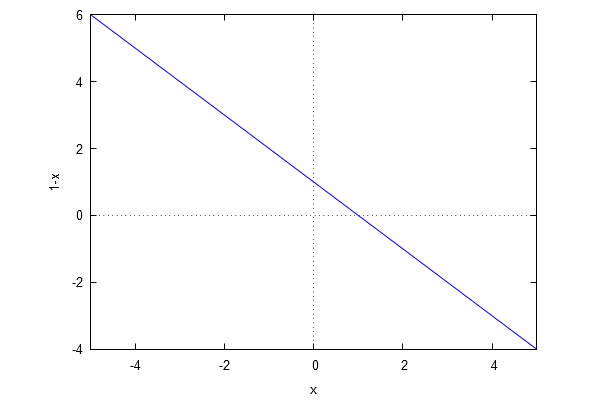
\includegraphics[width=1.1\linewidth]{FLT_n_1.png}
  \caption{Plot for $x^1 + y^1 = 1$}
  \label{fig:n_1}
\end{subfigure}%
\begin{subfigure}{.33\textwidth}
  \centering
  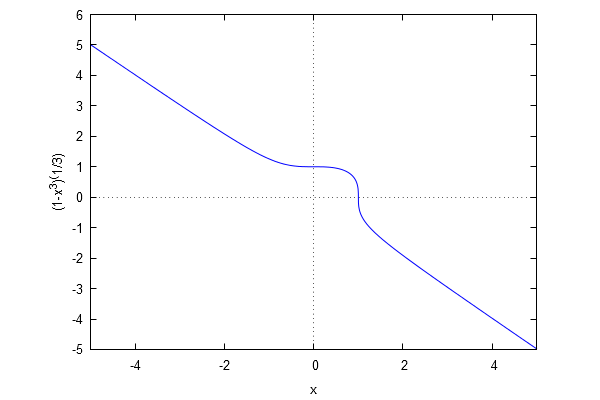
\includegraphics[width=1.1\linewidth]{FLT_n_3.png}
  \caption{Plot for $x^3 + y^3 = 1$}
  \label{fig:n_3}
\end{subfigure}
\begin{subfigure}{.33\textwidth}
  \centering
  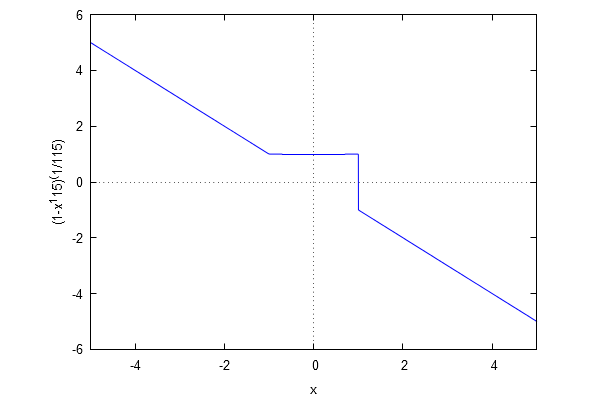
\includegraphics[width=1.1\linewidth]{FLT_n_115.png}
  \caption{Plot for $x^{115} + y^{115} = 1$}
  \label{fig:n_115}
\end{subfigure}
\caption{The higher the power the sharper the bump. For all three plots, vertical axis is $y$ and horizontal axis is $x$.}
\label{fig:FLT_n_odd}
\end{figure}
%

But that's not the only great division, even powers have all the same shape (which is different from the odd one), Fig.~\ref{fig:n_4}, except that the corners get sharper the higher the power, Fig.~\ref{fig:n_12}. The only exception to this is the Pythagorean equation $x^2 + y^2 = 1$ which is a circle and the only plot with maximum symmetry among $x^n + y^n = 1$.

One interesting thing here (thanks to Wildberger) is whether those curves actually exist, \eg for $x^3 + y^3 = 1$ the only rational solution is $(1,0), (0,1)$ this means that all other points on the curve are real numbers, however, the curves in Fig.~\ref{fig:n_3}, \ref{fig:n_115}, \ref{fig:FLT_n_even} are calculated by a computer program and we all know that computers can {\it not} process real numbers.

This seems to suggest that there is something special about Pythagoras, looks like ``no. 2" is actually number 1 :)
%
\begin{figure}
\centering
\begin{subfigure}{.5\textwidth}
  \centering
  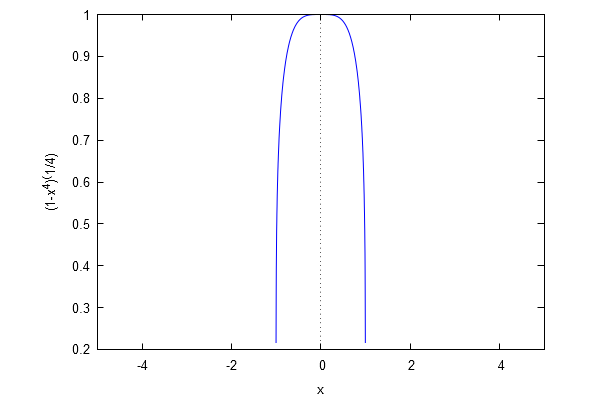
\includegraphics[width=1.1\linewidth]{FLT_n_4.png}
  \caption{Plot for $x^4 + y^4 = 1$}
  \label{fig:n_4}
\end{subfigure}%
\begin{subfigure}{.5\textwidth}
  \centering
  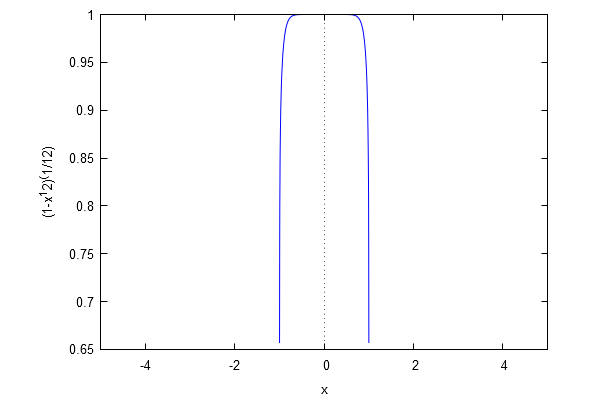
\includegraphics[width=1.1\linewidth]{FLT_n_12.png}
  \caption{Plot for $x^{12} + y^{12} = 1$}
  \label{fig:n_12}
\end{subfigure}
\caption{Sharper corners for sharper powers. For both plots, vertical axis is $y$ and horizontal axis is $x$.}
\label{fig:FLT_n_even}
\end{figure}
%

\bigskip\textbf{\textit{Idea \#1}}

Thanks to Wildberger's youtube videos the following ideas poped up in my head. The ancient greeks didn't use numbers like we do today, what we use are actually the arabic numerals. The greeks used line segments. To add one line segment on another you just join the two line segments to get a longer one. So I was curious as to what geometric meaning Fermat's last theorem presents us.

This prodded me to the idea that the angles between the two line segments (in the case where we are adding two numbers) actually means something. For example, in the case of $a^1 + b^1 = c^1$, we are adding two line segments $a$ and $b$ where the angles between them is $\pi/1$.

For the case of $a^2 + b^2 = c^2$, the angles between line segments $a$ and $b$ is actually $\pi/2$. Now how about the angle in $a^n + b^n = c^n$ with $n$ any arbitrary number $\ge 3$? is the angle between $a$ and $b$ given by $\pi/n$?

Using the cosine rule, the angle between line segments $a$ and $b$ is
%
\nbea
\cos \theta & = & \frac{(a^n + b^n)^{2/n} - a^2 - b^2}{-2 a b}
\neea
%
and its derivatives (if they mean anything) are given by
%
\nbea
\frac{d\cos \theta}{dn} & = & {{\left( {{b}^{n}}+{{a}^{n}}\right) }^{\frac{2}{n}}}\cdot \left( \frac{2\cdot \left( {{b}^{n}}\cdot \mathrm{log}\left( b\right) +{{a}^{n}}\cdot \mathrm{log}\left( a\right) \right) }{\left( {{b}^{n}}+{{a}^{n}}\right) \cdot n}-\frac{2\cdot \mathrm{log}\left( {{b}^{n}}+{{a}^{n}}\right) }{{{n}^{2}}}\right) \\
\frac{d\cos \theta}{da} & = & \frac{{{\left( {{b}^{n}}+{{a}^{n}}\right) }^{\frac{2}{n}}}-{{b}^{2}}-{{a}^{2}}}{2\cdot {{a}^{2}}\cdot b}-\frac{2\cdot {{a}^{n-1}}\cdot {{\left( {{b}^{n}}+{{a}^{n}}\right) }^{\frac{2}{n}-1}}-2\cdot a}{2\cdot a\cdot b} \\
\frac{d\cos \theta}{db} & = & \frac{{{\left( {{b}^{n}}+{{a}^{n}}\right) }^{\frac{2}{n}}}-{{b}^{2}}-{{a}^{2}}}{2\cdot a\cdot {{b}^{2}}}-\frac{2\cdot {{b}^{n-1}}\cdot {{\left( {{b}^{n}}+{{a}^{n}}\right) }^{\frac{2}{n}-1}}-2\cdot b}{2\cdot a\cdot b}
\neea
%
The above exercise yields a provocative result. To simplify the problem, we can ask if $r_1^n + 1 = r_2^n$ has rational solutions $r_1 \equiv a/b$ and $r_2 \equiv c/b$. This normalization seems a bit odd at first. But it is actually easier to visualize things this way if one thinks of $r_1, 1,$ and $r_2$ as sides of a triangle with $r_2$ the longest side among the three. This way one of the sides of the triangle is fixed to $1$ while we vary the other two sides.
%
\begin{figure}
\centering
\begin{subfigure}{.5\textwidth}
  \centering
  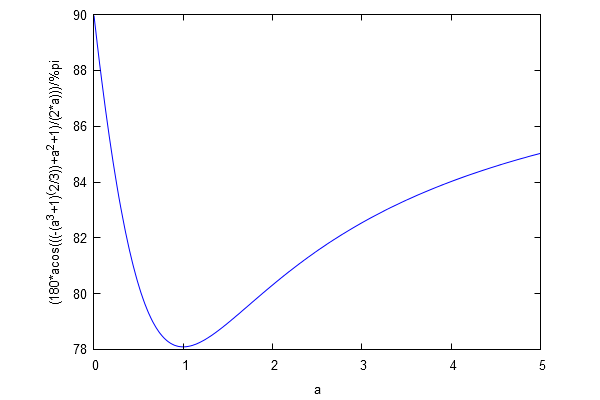
\includegraphics[width=1.1\linewidth]{FLT_angle_n_3.png}
  \caption{Angle plot for triangle $(a, 1, \sqrt{a^3 + 1^3})$}
  \label{fig:angle_n_3}
\end{subfigure}%
\begin{subfigure}{.5\textwidth}
  \centering
  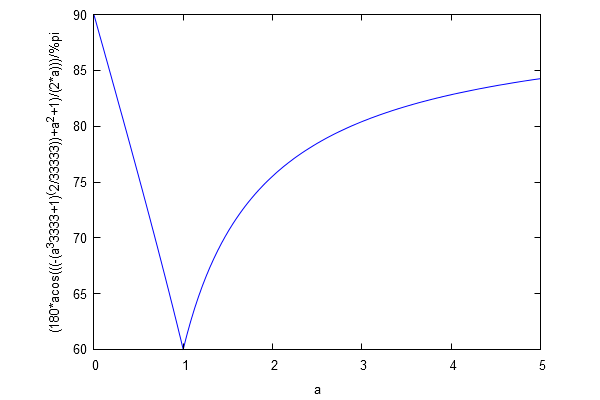
\includegraphics[width=1.1\linewidth]{FLT_angle_n_33333.png}
  \caption{Angle plot for $(a, 1, \sqrt{a^{33333} + 1^{33333}})$}
  \label{fig:angle_n_33333}
\end{subfigure}
\caption{For both plots, vertical axis is the angle between the 2 sides of triangle $a$ and $b$ with a fixed $b$ normalized to $1$}
\label{fig:FLT_angle}
\end{figure}
%

The angle $\theta$ between $a$ and $b$ is {\it not} fixed for $n \ge 3$. The angle always starts off at $90^\circ$ when $r_1 = 1$ and will quickly plummet as $r_1$ increases, Fig.~\ref{fig:angle_n_3}. It will then climb back up {\it asymptotically} to $90^\circ$. As we go higher in $n$, the initial dip and rebound will become more drastic but the overall behavior will remain the same, Fig.~\ref{fig:angle_n_33333}. So there is a clear dichotomy of the behavior of the angle for $n=1,2$ and $n \ge 3$.

As I was thinking about what this might mean I was reminded of Galois theory (you might want to check Wildberger's youtube lecture on this as an introduction, see his history of mathematics series). The reason why quintic equations have no solution is because the symmetry structure does not cascade as it does for quartic and below. Can it be that a symmetry structure plays a role here as well? If so, what kind of symmetry?

Since the triangle formed by $a$, $b$, and $c$ is a right triangle only for $n=2$ I imagine it has something to do reflection symmetry with respect to the $x$ and $y$ axes in the cartesian coordinate. Say the triangle is given by these three points $(0, 0)$, $(a, 0)$, and $(0, b)$, by doing horizontal and vertical reflections (plus translations) we can cover the entire cartesian plane, \eg a reflection w.r.t the $x$ axis generates the triangle $(0,0) (a,0) (0,-b)$ while a subsequent relection w.r.t the $y$ axis gives $(0,0) (-a,0) (0,-b)$. If we then translate this triangle using a vector $(a \hat x, b \hat y)$ - and combining it with our original triangle - we will get a rectangle $(0,0) (a,0) (a,b) (0,b)$, repeating this process indefinitely produces a covering for the entire cartesian plane.

Not so for $n \ge 3$, since the angle can never reach $90^\circ$ there is always some area that is not covered by the above symmetry operations. From this observation, the symmetry of interest is the discrete symmetry $Z_2$ (plus some translation symmetry).

\bigskip\textbf{\textit{Idea \#2}}

At this point I'm not sure what this all means, or if it is actually profitable to pursue this line of thought since I can't find anything concrete to say about it.

My next idea is whether there is a higher dimensional object that represents $a^n + b^n = c^n$ for different $n$'s. Since $n=2$ is a triangle maybe $n \ge 3$ is some 3d object (after all $a^3 + b^3$ means that we are adding two volumes to get a third one) and $n=4$ is an even higher dimensional object and so on. But again, I don't know what to make of it.

\bigskip\textbf{\textit{Idea \#3}}

I then was reminded of quantum mechanics. Before learning quantum mechanics I wouldn't even imagine of something that have discrete and continuum spectrum in one solution but there is (there are actually plenty examples in quantum mechanics). How is it related to Fermat? Because in Fermat, $a^n + b^n = c^n$ happens to just miss all of the integers $a,b,c$ for $n \ge 3$ (while taking in real values just fine). So these seems like the inverse hydrogen atom, instead of having discrete spectrum it has an inverse discrete spectrum where all integers are skipped (is there such a physical object in the universe?).

So maybe there's a differential equations that yield a solution where all integers are skipped? can we just do a Fourier transform of $a^n + b^n = c^n$? Just a wild guess :)

\bigskip\textbf{\textit{Idea \#4}}

Another strange idea I came up with was again inspired by symmetry. Say we move to the complex plane, does $a^n + b^n = c^n$ exhibit conformal symmetry? dilatation symmetry?

Why do they even relate to Fermat? It's all about angles! Back to idea \#1, the angles between the two line segments $a$ and $b$ is always fixed for $n=2$, this somewhat resembles conformal symmetry where the angle between two lines is always preserved. So maybe there's a conformal/dilatation symmetry preserved by $n=2$ which is not preserved by $n \ge 3$. Again, just a wild guess, nothing concrete :)

\bigskip\textbf{\textit{Fun Excursions}}

Since the above ideas didn't get me anywhere I was thinking about other aspects of Fermat. We know we can't find solutions with just two numbers $a$ and $b$, how many numbers do we need to get a solution? \ie $a^n + b^n  + d^n + \dots = c^n$.

So I began with $n=3$, and lo and behold, I found integer solutions for $a^3 + b^3  + d^3 = c^3$. Do these solutions have a pattern behind them? Euclid to the rescue $\dots$ (maybe)

\bigskip\textbf{\textit{Running along Euclid}}

Euclid (some people said it was the Babylonians) gave us an algorithm to find the solutions of $a^2 + b^2 = c^2$, which is as follows
%
\nbea
(m^2 - n^2)^2 + (2mn)^2 & = & (m^2 + n^2)^2
\neea
%
you simply pluck in whatever integers you fancy into $m$ and $n$ and Voila! you get a Pythagorean solution (one is usually interested in co-prime solutions, \ie $a,b,c$ have no common divisor). So maybe a similar algorithm exists for $a^3 + b^3  + d^3 = c^3$?

Well, there are actually plenty of algorithms for $a^3 + b^3  + d^3 = c^3$. They are categorized by how many parameters are used and more imprtantly by what solutions they produce, it turns out that the different algorithms generate only selective solutions or families unlike the Babylonian algorithm above which generate every solution for the Pyhtagorean equation.

The algorithm above is a two parameter algorithm, there is actually a one parameter algorithm as well. But before we discuss all this let me show you my misadventures with these algorithms as I try to wildly guess what they might be like.

\bigskip\textbf{\textit {Euclidean roullette}}

What we really want to know is how those Babylonians or Euclid came up with the formula (or they might have just been really smart and saw the solution immediately, me no Euclid). At a glance it looked like just a good guess. So let say we start with a simplest of most guesses
%
\nbea
a^2 + (a+y)^2  & = & (a + z)^2
\neea
%
we see that the solution for $a$ has to be
%
\nbea
(a + z)^2 - \left \{ (a+y)^2 + a^2 \right \} & = & z^2 + 2 a z - y^2 - 2 a y - a^2 = 0 \\
\rightarrow a & = & \pm \sqrt{2}\sqrt{z^2 - yz} + z - y
\neea
%
which in turn means that
%
\nbea
z^2 - yz & = & 2 w^2
\neea
%
for some integer $w$. One obvious solution is
%
\nbea
z & = & 2w \\
y & = & w \\
a & = & 2w + 2w - w = 3w \\
\rightarrow (3w)^2 + (4w)^2 & = & (5w)^2
\neea
%
And we get the $3,4,5$ solution and its integer multiples. There are actually many other solutions for $z^2 - yz = 2 w^2$, this turns out to be a blessing in disguise, we shall see this in a little bit.

Now, what happens if we choose a different starting point?
%
\nbea
a^2 + (a \cdot y)^2  & = & (a + z)^2 \\
(a + z)^2 - \left \{ (a \cdot y)^2 + a^2 \right \} & = & z^2 + 2 a z - a^2 y^2 = 0 \\
\rightarrow a & = &\frac{z \pm \sqrt{y^2 + 1}}{y^2}
\neea
%
This time, we can only solve it if we change $y$ into a rational number $p/q$ but solving $p^2/q^2 + 1 = r^2/s^2$ is just solving the Pythagorean equation in the first place. However, the above equation also means
%
\nbea
(a y^2 - z)^2 & = & y^2 + 1 \\
a^2 y^4 - 2 a y^2 z + z^2 & = & y^2 + 1 \\
a^2 p^4 - 2 a p^2 q^2 z + z^2 & = & p^2 q^2 + q^4
\neea
%
So why all this asinine substitutions?

\bigskip\textit{\textbf{Lagniappe}}

I wanted to say ``small lagniappe'' but lagniappe itself is already small :) The above two examples actually show us how to use Euclid's algorithm to solve other equations (instead of generating a new algorithm to solve the pyhtagorean equation). The first example
%
\nbea
z^2 - yz & = & 2 w^2
\neea
% 
can be paraphrased into the Pythagorean equation, because it was a consequence of
%
\nbea
a^2 + (a+y)^2 & = & (a+z)^2 \\
(m^2-n^2)^2 + (2mn)^2 & = & (m^2+n^2)^2
\neea
%
which means that
%
\nbea
a & = & m^2-n^2 \\
a + y & = & 2mn \\
a + z & = & m^2 + n^2
\neea
%
By solving the above equations, the algorithm for the solutions of $z^2 - yz = 2 w^2$ is then
%
\nbea
z = 2 n^2,~~ y = n^2 + 2mn -m^2, ~~w = n^2 (n - m)^2
\neea
%
\ie we can choose any two integers $m$ and $n$ and the integer solutions for $z^2 - yz = 2 w^2$ are given above (note that we can also choose $a = -(m^2 - n^2)$ generating a slightly different final result).

It's the same with $a^2 p^4 - 2 a p^2 q^2 z + z^2 = p^2 q^2 + q^4$, equating terms just like before gives
%
\nbea
a = m^2-n^2, ~~ z = 2 n^2,~~ y = \frac{p}{q} \rightarrow p = 2mn, q = m^2 - n^2
\neea
%
I called the above lagniappe because it was just a small boon. The boon is that there's actually a way to solve these seemingly random equations, \eg $z^2 - yz = 2 w^2$, $a^2 p^4 - 2 a p^2 q^2 z + z^2 = p^2 q^2 + q^4$. However, those solutions we found above are not unique because Euclid's algorithm itself is not unique, as we shall see.

There's also another fun thing related to this, if we start with
%
\nbea
(a+z)^2 + (a-z)^2 & = & (a \cdot y)^2 \\
(a+z)^2 + (a-z)^2 - (a \cdot y)^2 & = & -2 z^2 + a^2 y^2 - 2 a^2 = 0
\neea
%
we can now choose which one to solve
%
\nbea
{\rm solving ~} y:~ y & = & \pm \frac{\sqrt{2}\sqrt{z^2 + a^2}}{a} \\
{\rm solving ~} z:~ z & = & \pm \frac{a\sqrt{y^2 - 2}}{\sqrt{2}} \\
{\rm solving ~} a:~ a & = & \pm \frac{\sqrt{2}z}{\sqrt{y^2 - 2}}
\neea
%
note that we are not solving $y$ followed by $z$ followed by $a$, we are only solving {\it one} of them but since we have three variables we can choose which one to solve. We then have the following constraints
%
\nbea
{\rm from~solving~}y{\rm~we~get}:~~z^2 + a^2 & = & 2w^2 \\
{\rm from~solving~}z{\rm~or~}a{\rm~we~get}:~~2 u^2 + 2 & = & y^2
\neea
%
matching terms $(a+z)^2 + (a-z)^2 = (a \cdot y)^2 \rightarrow (m^2-n^2)^2 + (2mn)^2 = (m^2 + n^2)^2$
%
\nbea
a & = & m^2-n^2 + 2mn \\
z & = & m^2-n^2 - 2mn \\
y & = & \frac{2(m^2 + n^2)}{m^2-n^2 + 2mn} \\
\rightarrow w & = & m^2 + n^2 \\
\rightarrow u & = & \frac{n^2 + 2mn - m^2}{n^2 - 2mn - m^2}
\neea
%
Note that we have inserted factor of 2 where convenient :) It is now obvious that we can play this game forever, just substitute any function you fancy into the Pythagorean equation and match terms, just be careful about factors of 2.

The moral of the story here is that the Babylonians actually gave us quite a powerful tool to solve deophantine equations (if we can massage them into the Pythagorean one), these ancient people were not just good at building towers :) But in a broader sense it means that we can map one Diophantine equation into a simpler one, which is good.

\bigskip\textbf{\textit{Euclidean bulldozer}}

We now come back to the subject of utilizing unsophisticated guesses in meting out algorithms such as Euclid's. The first attempt above $a^2 + (a+y)^2 = (a+z)^2$ wasn't fruitful and in a glance this should be the same as $(a+x)^2 + (a+y)^2 = (a+z)^2$ since we can always shift $a+x \rightarrow a$. However, it is not true. Adding an extra degree of freedom like $x$ is a big deal, how big? let's see.

We can by brute force find an algorithm for $a^2 + b^2 = c^2$ from the most generic starting point
%
\nbea
(a+z)^2 & = & (a+x)^2 + (a+y)^2 \\
(a+z)^2 - \{(a+x)^2 + (a+y)^2\} & = & z^2+2az-y^2-2ay-x^2-2ax-a^2 = 0
\neea
%
Now we have four choices, we can solve for either, $a$, $x$, $y$, or $z$, which one we solve determines our fate. Solving for $a$ gives
%
\nbea
a = z-y-x \pm \sqrt{2}\sqrt{z^2+(-y-x)z+xy}
\neea
%
which means that
%
\nbea
z^2+(-y-x)z+xy & = & 2 p^2 \\
\rightarrow x & = & \frac{z^2-yz-2p^2}{z-y} \\
\rightarrow a & = & -\frac{(y+2|p|)z-y^2-2|p|y-2p^2}{z-y}
\neea
%
and there we have it, the full algorithm is
%
\nbea
\begin{array} {l c l c l}
a + x & = & z-y-2|p| & \rightarrow & (z-y-2|p|)(z-y) \\
a + y & = & -\frac{2|p|z-2|p|y-2p^2}{z-y}  & \rightarrow & 2|p|z-2|p|y-2p^2 \\
a + z & = & \frac{z^2+(-2y-2|p|)z+y^2+2|p|y+2p^2}{z-y}  & \rightarrow & z^2+(-2y-2|p|)z+y^2+2|p|y+2p^2
\end{array}
\neea
%
we can multiply each term by $(z-y)$ if we want to and flip the minus sign. So apparently we can just go by brute force to bulldoze out an algorithm, in this case we have {\it three} final degrees of freedom.

However, we can also solve $x$ first
%
\nbea
x & = & -a \pm \sqrt{z^2+2az-y^2-2ay}
\neea
%
The next step is crucial, do we solve for $a$ or $y,z$? Let's see, solving for $a$ gives
%
\nbea
a & = & -\frac{z^2-y^2-p^2}{2z-2y}
\neea
%
which is all well and good. Had we chosen to solve for $y$ we'd have gotten
%
\nbea
y & = & -a \pm \sqrt{z^2+2az-p^2+a^2}, ~~{\rm solving~for~}a~{\rm next} \\
\rightarrow a & = & -z \pm \sqrt{q^2+p^2} ~~~{\rm OR~solving~for~}z~{\rm next}\\
\rightarrow z & = & -a \pm \sqrt{q^2+p^2}
\neea
%
Solving either $a$ or $z$ produces no headway since now we have to solve for $q^2+p^2 = r^2$ which is our original problem. Thus the order we choose to solve the degrees of freedom matters. Can we follow the same mechanical steps to arrive at algorithms for $a^3 + b^3 + c^3 = d^3$?

\bigskip\textbf{\textit{Cubic conundrum}}

Applying the same guessing strategy to $a^3 + b^3 + c^3 = d^3$ turns out to be tricky. My first attempt was $a^3 + (a+y)^3 + (a+z)^3 = (a+w)^3$ but the cube root of a square root (generated by solving $a$ in terms of $y,z,w$) was too hard to handle.

The next natural progression is of course $(a+x)^3 + (a+y)^3 + (a+z)^3 = (a+w)^3$ to allow more flexibility but just like the preceding attempt the resulting equations quickly became intractable. My next attempt was to simplify things by adding a minus sign $(a+x)^3 + (-a+y)^3 + (a+z)^3 = (a+w)^3$ such that we no longer have $a^3$, however even with this modification the equations were still too long to be discernible
%
\nbea
&& (a+w)^3 - \{(a+x)^3 + (-a+y)^3 + (a+z)^3 \} = 0\\
&& ~~~~~~~~~~~\Longrightarrow a ~~= ~ (6z+6y+6x-6w)^{-1} (-3z^2+3y^2-3x^2+3w^2 \\
&& ~~~~~~~~~~~~~~~~~~~~~~~~~~~~ \pm \sqrt{3} (-z^4+(-4y-4x+4w)z^3+(-6y^2+6x^2-6w^2)z^2+ \\
&& ~~~~~~~~~~~~~~~~~~~~~~~~~~~~ (-4y^3-4x^3+4w^3)z-y^4 + (4w-4x)y^3+(6w^2-6x^2)y^2+ \\
&& ~~~~~~~~~~~~~~~~~~~~~~~~~~~~ (4w^3-4x^3)y-x^4+4wx^3-6w^2x^2+4w^3x-w^4 )^{1/2})
\neea
%
here we have a super long square root (no more cube root since we have no $a^3$). The problem with this square root is that it contains fourth powers $z^4, y^4, x^4$. Solving for $x, y$ or $z$ inside the square root generates more problems, \ie roots containing higher powers which in turn generates more complicated equations.

My final attempt was $(a+x)^3 + (-b+y)^3 + (b+z)^3 = (a+w)^3$ however, solving $a$ or $b$ still generates ridiculously long square roots, solving for $x$ however seems to be a lot simpler
%
\nbea
x & = & (-z^3-3az^2-3a^2z-y^3-3by^2-3b^2y+w^3+3aw^2+3a^2w-b^3)^{1/3}+b
\neea
%
We are now faced with the same decision tree as discussed previously, who's next? Turns out that solving for $y,z$ or $w$ generates $p^3+q^3+r^3 = s^3$ just like the Pythagorean case above. Seems like we need to solve $b$ or $a$ first but $b$ gives a better outcome
%
\nbea
b & = & (-z^3-3az^2-3a^2z+w^3+3aw^2+3a^2w-p^3)^{1/3}+y
\neea	
%
It looks good as $y$ decouples. Next we need to solve for $a$, solving any other variables generates $p^3+q^3+r^3 = s^3$
%
\nbea
a & = & \left (3z^2-3w^2 \pm \sqrt{3}\sqrt{-z^4+4wz^3-6w^2z^2+(4w^3-4q^3-4p^3)z-w^4+(4q^3+4p^3)w} \right ) \times \\
&& (6z-6w)^{-1}
\neea	
%
That long square root is a killer, solving it for $z$ or $w$ generates a root of a cube root of a root of a root, {\it four} nested roots! {\it Q.E.D} ({\it Q}.uickly {\it E}.nded {\it D}.reams)

In short, a brute force guessing game might be theoretically possible but not recommended :) in other words, it works well for certain obvious cases and thus it only has a very limited merit.

\bigskip\textbf{\textit{Euclidean apery}}

We now go back to guessing our own version of an algorithm for the Pythagorean equation (without a bulldozer). In our case, the goal here is to solve $a$ in terms of two completely free parameters $z$ and $y$. Let's try one with a quite generic structure
%
\nbea
(a - z)^2 + (a\cdot y)^2  & = & (a + z)^2 \\
(a + z)^2 - \left \{ (a \cdot y)^2 + (a - z)^2 \right \} & = & 4 a z - a^2 y^2 = 0 \\
\rightarrow a & = & \frac{4 z}{y^2}
\neea
%
Yay! It works! (the other solution is $a=0$). The full solution is then
%
\nbea
\left ( \frac{4 z}{y^2} - z\right )^2 + \left ( \frac{4 z y}{y^2} \right )^2 & = & \left ( \frac{4 z}{y^2} + z\right )^2 \\
\Rightarrow \left ( 4 z - z y^2\right )^2 + \left ( 4 z y \right )^2 & = & \left ( 4 z + z y^2\right )^2
\neea
%
Although this is different from Euclid's, given any integer $z$ and $y$ we can generate a solution. Looks like these algorithms are not unique (as advertised) although I'm not sure (or too lazy to prove) that this version covers all solutions of the Pythagorean equation.

A more straighforward guess will be
%
\nbea
(a + z)^2 - (a - z)^2 & = & 4az
\neea
%
we can simply promote $a \to a^2, z \to z^2$ to get
%
\nbea
(a^2 + z^2)^2 - (a^2 - z^2)^2 & = & 4a^2z^2 = (2az)^2
\neea
%
which is Euclid's (or the Babylonians').

So the trick in this guessing game is that you guess a term on the LHS and another on the RHS. You then want the difference between those two sides {\it not} to be a sum of terms, because then you're just going back to square one by needing to solve some equation in the form of $x_1^{n_1} + x_2^{n_2} = a^m$. For example, if you're naively try to solve fermat's cubic last theorem the same way
%
\nbea
(a-z)^3 + X^3 & = & (a+z)^3 \\
\rightarrow X^3 & = & 2z^3 + 6a^2 z
\neea
%
You just get another deophantine equation to solve, back to square one.

One thing to note here is that we at first assume that all terms in our guess has the same power, \eg $a, z$ both have the power of one, we can for example promote things to $a^n, z^m$ but our goal for now is to see how far these simple guesses take us.

\bigskip\textbf{\textit{Jabs in the dark}}

We now begin our journey in guessing the form of algorithm for $a^3 + b^3 + c^3 = d^3$.
\begin{enumerate}
\item I first tried the following solution (which looks simplest of all)
%
\nbea
a^3 + b^3 + K^3  & = & (a + b)^3
\neea
%
with some unknown integer $K$ (in Euclid's case $K$ is just $2mn$). Let's see if we get lucky. Now $K^3$ is obviously $3 a b (b + a)$. Sadly, the only solution is $a = 1$, $b = 8$, $K=6$ and their integer multiples. 

We can try setting $a = 3^2 c^3$. First, why this choice? The goal here is to make $3a$ into $3a=P^3$ for some integer $P$. So the first thing to do is to complete the factor 3 into $3^3$ by multiplying it by $3^2$. What we need next is $b (b + a) = N^3$ which we will solve later. With this choice $3 a b (b + a) = 3^3 c^3 N^3 = K^3 \rightarrow K = 3 c N$ we would have found our algorithm. However, even with this scheme, the only solutions are integer multiples of $a = 1$, $b = 8$, $K=6$.

\item From the list of solutions for $a^3 + b^3 + c^3 = d^3$ I saw a familiar face $3, 4, 5, 6$ (by the way, the tuplet $3,4,5,6$ also represent the sides of a right triangle $3,4,5$ with an area of $6$). Prompting me to guess a solution of the form
%
\nbea
a^3 + (a+1)^3 + (a+2)^3  & = & (a + 3)^3 \\
(a + 3)^3 - (a^3 + (a+1)^3 + (a+2)^3) & = & 2 (3 - a) (a^2 + 3a + 3) = 0
\neea
%
The last equation shows that this scheme will only work for $a = 3$, no other solution is sequential.

\item What if we mix products and additions of terms? Like this one
%
\nbea
a^3 + (a \cdot x)^3 + (a \cdot y)^3 & = & (a + z)^3 \\
(a + z)^3 - \left \{ a^3 + (a \cdot x)^3 + (a \cdot y)^3 \right \} & = & z^3 + 3 a z^2 + 3 a^2 z - a^3 y^3 - a^3 x^3
\neea
%
Now this doesn't look promising to some since we can always factor out $a$ to get $y^3 + x^3 + 1 = w^3$, however, from our previous discussion about shifting $a + z \to a$, we know that adding a degree of freedom actually makes a difference. So let give this a shot. The solution is
%
\nbea
a & = & \frac{z \left \{ (y^3 + x^3 + 1)^{2/3} + (y^3 + x^3 + 1)^{1/3} +1 \right \} }{(y^3 + x^3) }
\neea
%
while the other two solutions give imaginary $a$. Which is rather disappointing since we now need to solve
%
\nbea
y^3 + x^3 + 1 & = & w^3
\neea
%
so this time adding a degree of freedom doesn't help. If we insist in substituting the solution for $a$ the factor $z$ cancels from both LHS and RHS and the only free variables in $a^3 + (a \cdot x)^3 + (a \cdot y)^3 = (a + z)^3$ are just $x$ and $y$ which is the same free variables we have in $y^3 + x^3 + 1 = w^3$.

At this point I would like to list solutions of $y^3 + x^3 + 1 = w^3$, see Table~\ref{Tab:1} (sorted in ascending $x$). One can immediately see that $y=138$ gives us {\it two} different sets of solutions ($426$ also gives two solutions but once as $x$ and another as $y$). Also, from their prime factors we can see that the solutions are all co-prime to one another.

Another thing to note is that the difference $y-x$ and $w-y$ are all different for different solutions, showing that an algorithm, \ie $a^3 + (a+m)^3 + (a+n)^3 = (a + p)^3$ where $m,n,p$ are {\it fixed} will not work as each fixed difference $m,n,p$ will only give a single solution. 

In addition, this also means that it is a near miss for Fermat, $a^3 + b^3 = c^3$ has no solutions but $1 + a^3 + b^3 = c^3$ does :)

One last comment on this topic, we can arrange things differently $y^3 + x^3 + 1 = w^3 \rightarrow y^3 + x^3 = w^3 - 1$
%
\nbea
y^3 + x^3 & = & w^3 - 1 \\
& = & (w-1)(w^2+w+1) \\
& = & (w-1)((w-1)^2+3w) \\
& = & (w-1)^3 + 3w(w-1)
\neea
%
We can now add degrees of freedom as usual $y = b+z, ~ x = b-z$
%
\nbea
(b+z)^3 + (b-z)^3 & = & (w-1)^3 + 3w(w-1) \\
6bz^2+2b^3 & = & (w-1)^3 + 3w(w-1)
\neea
%
This looks promising as we have the same number of terms in both LHS and RHS. We know that $2b^3$ can't be $u^3$ for some integer $u$ due to the factor of 2, the easiest algorithm for $y^3 + x^3 + 1 = w^3$ is to set $2b^3 = 3w(w-1), ~ 6bz^2 = (w-1)^3$. However, from the $1,6,8,9$ solution it is clear that we cannot make such identification.

We can try adding more variables, \eg $1=(b-z-a), y=(b+z)$, but this only complicates things with no clear benefit. In other words, only the combination, \eg $6bz^2+2b^3$, constitutes $x_1^3 + x_2^3$, we cannot cast any one term $6bz^2$ or $2b^3$ as a pure power of 3, $6bz^2 = p^3$ or $2b^3 = q^3$.

\item Another potential solution is
%
\nbea
(a-b)^3 + (b-c)^3 + (c-a)^3 & = & 3 (a-b)(b-c)(c-a)
\neea
%
The nice thing is that the RHS is not a sum of terms, so we have a chance if we set
%
\nbea
(a-b)(b-c)(c-a) & = & 3^2 w^3
\neea
%
To simplfy things let's denote $p = (a-b)$, $q = (b-c)$, $r = (c-a)$
%
\nbea
p \cdot q \cdot r & = & 3^2 w^3\\
p + q+ r & = & 0
\neea
%
We can solve the above equations by substituting $p = 3^2 w^3/qr$ into $p + q+ r = 0$
%
\nbea
0 & = & 3^2 w^3 + q^2 r + q r^2 \\
\rightarrow r & = & \frac{-q^2 \pm \sqrt{q^4 - 36 \cdot q \cdot w^3}}{2 q}
\neea
%
To ensure that $r$ is an integer, $q^4 - 36 q w^3 = v^2$ for some integer $v$. The interesting thing is that there are only two solutions I can find for this to happen
%
\nbea
q \rightarrow q,~w\rightarrow -2q & ~:~ & q^4 - 36 q (-2q)^3 = 289 q^4 = (17 q^2)^2 \\
q \rightarrow 4q,~w\rightarrow -q & ~:~ & (4q)^4 - 36 (4q) (-q)^3 = 400 q^4 = (20 q^2)^2 
\neea
%
Regrettably this provision will only give one solution
%
\nbea
(8q)^3 + (q)^3 + (-9q)^3 & = & (-6q)^3
\neea
%
which is just a multiple of the $1,6,8,9$ solution.

We can do some minor rearrangement
%
\nbea
p^3 + q^3 + 3 p q (p+q) & = & (p+q)^3 \\
\to (3p^3)^3 + (3q^3)^3 + (3 p q z)^3 & = & (z^3)^3 ~~~z^3 = 3p^3 + 3q^3~~~{\rm OR}\\
\to (3^2p^3)^3 + (q^3)^3 + (3 p q z)^3 & = & (z^3)^3~~~z^3 = 3^2p^3 + q^3~~~{\rm OR}\\
\to (3p^3)^3 + (q^3)^3 + (3 p q z)^3 & = & (z^3)^3~~~3z^3 = 3p^3 + q^3~~~{\rm OR}\\
\to p^3 + q^3 + z^3 & = & (p+q)^3~~~z^3 = 3 p q(p+q)
\neea
%
we can either lump the factor of $3^2$ into one of the variables or spread it onto any two of them or  assume the whole thing $3 p q(p+q)$ is a power of three $z^3$. I got some interesting result from this exercise, \eg the {\it largest} solution I found from this simple guessing game is
%
\nbea
59707533^3 + 2268747144^3 + 981751158^3 & = & 2328454677^3
\neea
%
this one was from $p \to 3 p^3, ~ (p+q) \to 3 u^3$.

\item Another promising solution is 
%
\nbea
(m-n)^3 + n^3 + A^3 & = & (m+n)^3 \\
\rightarrow A^3 & = & n^3 + 6 m^2 n
\neea
%
We can solve for $m$ or $n$ or $A$, but $m$ seems to yield the easiest solution, which is
%
\nbea
m & = & \pm \sqrt{\frac{\frac{A^3}{n} - n^2}{6}}
\neea
%
Sadly, this only gives 2 integer solutions, they are
%
\nbea
m-n = 17 ~~~ n = 4 ~~~ A = 22 ~~~ m+n = 25 \\
m-n = -2 ~~~ n = 9 ~~~ A = 15 ~~~ m+n = 16
\neea
%
I was hoping that these conditions, \eg $m = \pm \sqrt{\frac{\frac{A^3}{n} - n^2}{6}}$ or $r = \frac{-q^2 \pm \sqrt{q^4 - 36 \cdot q \cdot w^3}}{2 q}$ would yield a class of integer solutions instead of just one (or two).

So it looks like there's really no solution for $a^3 + b^3 + c^3 = d^3$ if we start we just simple guesses. 



\end{enumerate}


















%
\begin{table}[]
\centering
\caption{$(x)$ means prime factors of $x$}
\label{Tab:1}
\begin{tabular}{|c|c|c|c|c|c|}
\hline
$x$ & $y$ & $w$ & $(x)$ & $(y)$ & $(w)$ \\ \hline 
6 & 8 & 9 & $(2, 3)$ & $(2^3)$ & $(3^2)$ \\
71 & 138 & 144  & $(71)$ & $(2,3,23)$ & $(2^4, 3^2)$ \\
135 & 138 & 172  & $(3^3, 5)$ & $(2,3,23)$ & $(2^2, 43)$ \\
236 & 1207 & 1210  & $(2^2,59)$ & $(17,71)$ & $(2,5,11^2)$ \\
242 & 720 & 729  & $(2, 11^2)$ & $(2^4, 3^2, 5)$ & $(3^6)$ \\
372 & 426 & 505  & $(2^2,3,31)$ & $(2,3,71)$ & $(5,101)$ \\
426 & 486 & 577  & $(2,3,71)$ & $(2,3^5)$ & $(577)$ \\
566 & 823 & 904  & $(2,283)$ & $(823)$ & $(2^3,113)$ \\
575 & 2292 & 2304  & $(5^2,23)$ & $(2^2,3,191)$ & $(2^8,3^2)$ \\
791 & 812 & 1010  & $(7,113)$ & $(2^2,7,29)$ & $(2,5,101)$ \\
1124 & 5610 & 5625  & $(2^2,281)$ & $(2,3,5,11,17)$ & $(3^2,5^4)$ \\
1938 & 2820 & 3097  & $(2,3,17,19)$ & $(2^2,3,5,47)$ & $(19,163)$ \\
1943 & 6702 & 6756  & $(29,67)$ & $(2,3,1117)$ & $(2^2,3,563)$ \\
2196 & 5984 & 6081  & $(2^2,3^2,61)$ & $(2^5,11,17)$ & $(3,2027)$ \\
2676 & 3230 & 3753  & $(2^2,3,223)$ & $(2,5,17,19)$ & $(3^3,139)$ \\ \hline
\end{tabular}
\end{table}
%

\bigskip\textbf{\textit{Expanding the horizon}}

Finding a generic algorithm for $a^3 + b^3 + c^3 = d^3$ just by guessing seems to be quite problematic as we have seen above. So what if we add another number? Say
%
\nbea
a^3 + b^3 + c^3 + d^3 & = & e^3
\neea
%
Going back to our symmetrical solution
%
\nbea
(a-z)^3 + \Delta & = & (a+z)^3 \\
\rightarrow (a+z)^3 - (a-z)^3 = \Delta & = & 2z^3 + 6a^2 \\
\Delta & = & z^3 + z^3 + 6a^2 z
\neea
%
so as long as $a^2 = 6^2 w^6$ and $z = v^3$ the above solution works since every term is a power of 3. The full solution is then
%
\nbea
(a^3 - 6^2 b^6)^3 + (6^2 b^6)^3 + (6^2 b^6)^3 + (a^2 \cdot 6 b^2)^3  & = & (a^3 + 6^2 b^6)^3
\neea
%
But I don't like this solution since it contains a constant factor $2$. There's yet another solution, if we began with
%
\nbea
(-a+b+c)^3 + (a-b+c)^3 + (a+b-c)^3 + X & = & (a+b+c)^3\\
\rightarrow X & = & 24 a b c
\neea
%
The above approach works as there is a so called ``symmetry'' where all complicated terms cancel for LHS and RHS. This was done by alternating the minus sign in each term to make sure there is only one $a^3, b^3, c^3$ on the LHS as there is on the RHS. Now, since $X$ is just a product of terms the most obvious choice would be $a \rightarrow a^3, b \rightarrow b^3, c \rightarrow 3^2 c^3$. The full solution is then
%
\nbea
(-a^3 + b^3 + 3^2 c^3)^3 + (a^3 - b^3 + 3^2 c^3)^3 + (a^3 + b^3 - 3^2 c^3)^3 + (2 \cdot 3 \cdot a b c)^3  & = & (a^3 + b^3 + 3^2 c^3)^3
\neea
%
There are other choices as well like $a \rightarrow a^3, b \rightarrow 3 b^3, c \rightarrow 3 c^3$. A more generic solution would be $a \rightarrow a^{3 \cdot m_1}, b \rightarrow 3 \cdot K_1^{3 \cdot n_1} b^{3 \cdot m_2}, c \rightarrow 3 \cdot K_2^{3 \cdot n_2} c^{3 \cdot m_2}$ but this also allows for something else, namely $a^3 + b^3 + c^3 + d^N = e^3$ by setting $a \rightarrow 2^{N-3} 3^{N-1} a^{N},~2^3 \cdot 3~ abc \rightarrow 2^3 \cdot 3~ (2^{N-3} 3^{N-1} a^{N}) b^{N} c^{N}  = (2 \cdot 3~abc)^N$, \ie
%
\nbea
(2^{N-3} 3^{N-1} a^{N} + b^N + c^N)^3 & = & (-2^{N-3} 3^{N-1} a^{N} + b^N + c^N)^3 + (2^{N-3} 3^{N-1} a^{N} - b^N + c^N)^3 + \\
&& (2^{N-3} 3^{N-1} a^{N} + b^N - c^N)^3 + (2 \cdot 3 a b c)^N
\neea
%

The most general solution would be to distribute the prime factors of $P^3 (\equiv 24 abc)$ into $a$, $b$, and $c$,
%
\nbea
P = \prod_{i=1}^{L} p_i^{n_i} ~~~\longrightarrow~~~ P^3 = \prod_{i=1}^{L} p_i^{3 n_i}
\neea
%
where each $p_i$ is a prime number, $n_i$ the multiplicity of $p_i$ and $L$ the number of different prime factors of $P$ and the probability is infinite :)

One way we can use our newly found expanded horizon is to set one of the terms, $(-a+b+c)$ or $(a-b+c)$ or $(a+b-c)$, to zero, since we can't set the product term $24abc$ to zero without resulting in a trivial pursuit :)

By setting one of the terms above to zero we would get our prime objective $a^3 + b^3 + c^3 = e^3 $ from $a^3 + b^3 + c^3 + \cancel{d^3} = e^3$. However, this exercise proves futile as the only solution generated is the infamous $1,6,8,9$, \ie $a = 1, b = 2, c = 1 \rightarrow -9a^3 + b^3 + c^3 = 0$.

There is a  possible (and potential) use of the above algorithm. Say we start with $(a+z)^3$ and $(a+y)^3$ on the LHS and RHS respectively, what we want is
%
\nbea
(a+z)^3 & = & (a+y)^3 + C_1^3 + C_2^3 \\
(a+z)^3 - (a+y)^3 & = & 3 a^2 z + 3 a z^2 + z^3 - (3 a^2 y + 3 a y^2 + y^3) \\
& = & 3 a^2 z + 3 a z^2 - y^3 - (3 a^2 y + 3 a y^2 - z^3) \\
& = & (a+z)^3 - a^3 - z^3 - y^3 - ((a+y)^3 - a^3 - y^3 - z^3) \\
& = & C_1^3 - C_2^3 \\
\rightarrow C_1^3 & = & (a+z)^3 - a^3 - z^3 - y^3 \\
\rightarrow C_2^3 & = & (a+y)^3 - a^3 - y^3 - z^3
\neea
%
in the second line we need to swap $y \leftrightarrow z$ otherwise we'll get
%
\nbea
3 a^2 z + 3 a z^2 + z^3 & = & (a+z)^3 - a^3 \\
\tilde C ^3 & = & (a+z)^3 - a^3
\neea
%
which is Fermat and we don't have a solution for it. However, we now have $a^3 + b^3 + c^3 + d^3 = e^3$ for both $C_1$ and $C_2$, the bad news is that we might not be able to use the algorithm found above to solve them. The main problem is that $C_2$ has the same terms as $C_1$ on the RHS. Another problem is, even if we only consider $C_1$, matching terms to our algorithm above
%
\nbea
(a+z) & = & -p^3 + q^3 + 3^2 r^3 \\
a & = & -p^3 + q^3 - 3^2 r^3 \\
z & = & -p^3 - q^3 + 3^2 r^3 \\
y & = & - 2 \cdot 3 ~ pqr
\neea
%
the solution will be
%
\nbea
r & = & \left ( \frac{q^3 + p^3}{9} \right )^{1/3} \\
a & = & 2 q^3 \\
y & = & 2~pq~3^{1/3} (q^3 + p^3)^{1/3} \\
z & = & -2(q^3 + p^3)
\neea
%
while $p$ and $q$ remain free parameters. The above requires that 
%
\nbea
q^3 + p^3 & = & \frac{w^3}{3}
\neea
%.
and the only solution is $q = 1,~p=2, ~w=3$ (this is just the 1,6,8,9 solution with $z=0$). We could have chosen our other algorithm, \ie $a+z = -p^3 + 3 q^3 + 3 r^3$ but this choice leaves us no way out. But why did we choose $(a+z) = -p^3 + q^3 + 3^2 r^3$ in the first place? because other choices generate complex solutions :)

\bigskip\textbf{\textit{Observation intermission}}

We now take a break from guessing and start staring at the numerical solutions of $a^3 + b^3 + c^3 = d^3$ we found and take stock of what we've found so far.

First, the solutions are not unique, we have pairs of numbers that appear in more than one solution, see Table.~\ref{Tab:2}.
%
\begin{table}[]
\centering
\caption{Some sample of twins for $x^3 + y^3 + z^3 = w^3$, including one of the biggest one I found (see bottom row)}
\label{Tab:2}
\begin{tabular}{||c c c c||}
\hline
$x$ & $y$ & $z$ & $w$ \\ \hline 
3 & 36 & {\bf 37} & {\bf 46} \\
27 & 30 & {\bf 37} & {\bf 46} \\ \hline
76 & 165 & {\bf 192} & {\bf 229} \\
102 & 157 & {\bf 192} & {\bf 229} \\ \hline
{\bf 9} & 58 & 255 & {\bf 229} \\
{\bf 9} & 183 & 220 & {\bf 229} \\ \hline
58 & {\bf 201} & 255 & {\bf 292} \\
183 & {\bf 201} & 220 & {\bf 292} \\ \hline
24 & 159 & {\bf 382} & {\bf 391} \\
87 & 150 & {\bf 382} & {\bf 391} \\ \hline
~2678 & 10533 & {\bf 43420} & {\bf 43629} \\
~~5157~~& ~~10166~~ & ~~{\bf 43420}~~ & ~~{\bf 43629}~~ \\ \hline
\end{tabular}
\end{table}
%
There are in total 1290 such twins from a total of 39607 solutions (around $3\%$, solutions are generated ascendingly by $x$, the smallest number in each solution). However, this percentage depends on how we search the solution space. Twins are more likely to pop up when $x, y, z$ are relatively close, see comments in ``Intuition rumination" section.

Moreover, there are intriguing solutions like this one, where the difference between the two largerst terms is just one!
%
\nbea
462^3 + 1981^3 + 51227^3 & = & 51228^3
\neea
%

\underline{\textit{\textbf{An interesting question will be:}}} the distribution of these twins, are they spread evenly? does their precentage keep fluctuating or does it stabilize at some point or does it increase without bound? For example see Fig.~\ref{fig:twins-dist}
%
\begin{figure}
\centering
  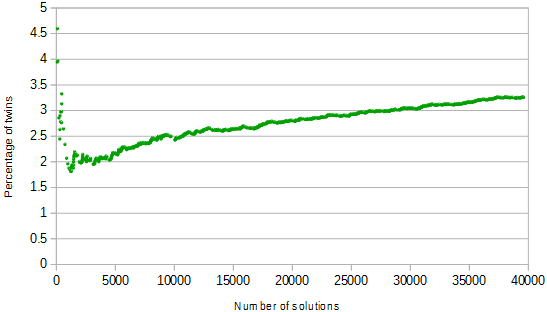
\includegraphics[width=.7\linewidth]{FLT_twins_dist.png}
  \caption{Plot of the distribution of twins among solutions of $a^3 + b^3 + c^3 = d^3$. Each green dot indicates where each twin was born among the solutions. First data point is excluded as first twins occur as solutions \#3 giving a distortedly high 33.3\% value.}
\label{fig:twins-dist}
\end{figure}
%

Second, guessing for an algorithm is not the best strategy here because there are four terms in total. It is hard to cancel terms between LHS and RHS that will result only in a product of terms as we can see from my attempts above, \eg
%
\nbea
(a+z)^3 - (a-z)^3 & = & 2 z^3 + 6 a^2 z
\neea
%
the factor of 2 in front of $z^3$ spoils everything because we need $2 z^3 = w^3$ for some integer $w$. What if we add more variables? say $(x + y +z)^3$, the problem is that there are three cubes on the RHS $x^3, y^3, z^3$ but we only have 3 terms on the LHS, this means that
%
\nbea
(x+\Delta_1)^3 + (y+\Delta_2)^3 + (z+\Delta_3)^3 & = & (x + y +z)^3
\neea
%
We can cancel $x^3, y^3,z^3$ on both sides but we now have $\Delta_1^3, \Delta_2^3, \Delta_3^3$ on the LHS (plus cross terms on both sides) that we cannot cancel.

Contrast this situation to $a^3 + b^3 + c^3 + d^3 = e^3$. If we start with $(x+y+z)^3$ on the RHS, we can cycle a minus sign on the LHS $(-x+y+z)^3$, $(x-y+z)^3$, $(x+y-z)^3$ and we will have exactly one $x^3$, $y^3$, $z^3$ on both sides with an extra term $d^3$ to absorb the rest of the cross terms. No such luck with just four terms $a^3 + b^3 + c^3 = d^3$, even if we start with two terms $(x+y)^3$ on the RHS the best I could get was
%
\nbea
(x+a)^3 + (y-a)^3 + 3 (x+a)(y-a)(x+y) & = & (x+y)^3
\neea
%
which was attempt \#4 with some minor rearrangement.

Speaking of attempt \#4 and \#5, we see something peculiar. Our usual observation says that we have  one less constraint than the number of degrees of freedom and so we should have a multitude of solutions instead of just one. Let's start with \#4, its constaints are
%
\nbea
p^3 + q^3 + r^3 & = & 3^3 w^3\\
p \cdot q \cdot r & = & 3^2 w^3\\
p + q+ r & = & 0
\neea
%
so we have 4 degrees of freedom $p,q,r,w$ with three constraints. For \#5, its {\it two} constraints are
%
\nbea
(m-n)^3 + n^3 + A^3 & = & (m+n)^3 \\
n^3 + 6 m^2 n & = & A^3
\neea
%
Again one extra free term, two constraints with {\it three} degrees of freedom $m,n,A$. The odd thing here is that the above two examples yield only one solution each, despite the extra {\it free} degree of freedom.

How can this be? This is because we are so used to thinking about real numbers. When solving a system of equations, the equations are the only constraints there are. Not so with integers/natural numbers. By requiring that the solutions are integers we are implicitly imposing another constraint, albeit a non traditional one. Going back to Fermat, $a^3 + b^3 = c^3$, we have only one constraint and three degrees of freedom and yet it has no solutions! It's because all the solutions are real numbers.

Let's see this in more detail through a concrete example

\bigskip\textbf{\textit{Attempt \#6 must die!}}

This one was exhilirating because at  a glance it gives you a lot of hope until you see it more closely. The starting point is
%
\nbea
a^3 + (y^{1/3})^3 + (a-z)^3 & = & (a + 8z)^3 \\
(a + 8z)^3 - \{a^3 + (y^{1/3})^3 + (a-z)^3\} & = & 513 z^3+189 a z^2+27 a^2 z-y-a^3 = 0
\neea
%
The funny term $(y^{1/3})^3$ is due to hindsight :) and even though in itself it is a constraint, it's irrelevant to the point I'm trying to make here. On the onset it seems like we have three degrees of freedom with only one constraint. Implying
%
\nbea
a & = & \left(\frac{\sqrt{1539648z^6-7344yz^3+y^2}}{2}-\frac{y-3672z^3}{2} \right)^{1/3} \\
&& +144z^2 \left ( \frac{\sqrt{1539648z^6-7344yz^3+y^2}}{2}-\frac{y-3672z^3}{2} \right)^{-1/3}+9z
\neea
%
To have any chance at all the inner square root has to produce an integer
%
\nbea
1539648z^6-7344yz^3+y^2 & = & u^2
\neea
%
but this is an additional constraint. One might object that it also introduces a new degree of freedom $u$. However, solving the above equation
%
\nbea
y=3672z^3 \pm \sqrt{11943936z^6+u^2}
\neea
%
This in turn means we acquire another constraint $\sqrt{11943936z^6+u^2}$ (which comes with another degree of freedom). This is a zero sum game, we are not gaining anything. We can continue with this forever!

Say we don't want to play this game, we can set
%
\nbea
1539648z^6-7344yz^3+y^2 & = & 0 \\
\rightarrow y & = & 216 z^3
\neea
%
which is good news because $216 = 6^3$ (another solution is $y = 7128 z^3$). However, by this time we have utilized two constraints, the original equation and $1539648z^6-7344yz^3+y^2 = 0$. This is no good. To see why, let's continue. 

We have one more constraint to solve, $((y-3672z^3)/2)^{1/3}$ has to be an integer, the solution is $z = -w/12$ for some integer $w$. This looks promising, we have a degree of freedom, but if you substitute this solution, $z = -w/12, ~ y = 216 z^3 = -w^3/8, ~ a = -11w/4$, \ie all terms in $a^3 + (y^{1/3})^3 + (a-z)^3 = (a + 8z)^3$ are just multiples of $w$
%
\nbea
\left ( \frac{-11 w}{4} \right )^3 + \left ( \frac{- w}{2} \right )^3 + \left ( \frac{-8 w}{3} \right )^3 & = & \left ( \frac{-41 w}{12} \right )^3 \\
\rightarrow 33^3 + 6^3 + 32^3 & = & 41^3
\neea
%
Sadly we only get one final solution $6,32,33,41$ because we have three degrees of freedom to begin with but utilize three constraints to get a solution, $a^3 + (y^{1/3})^3 + (a-z)^3 = (a + 8z)^3, ~\sqrt{11943936z^6+u^2}, ~((y-3672z^3)/2)^{1/3}$. Thus the requirement that the solutions are integers is itself a powerful constraint!

Another thing to note about the example above is that since the solution for a cubic polynomial is a cube root of a square root, $( \dots + \sqrt{\dots})^{1/3}$, we immediately incur two constraints, one for each root.

One quick side note, I initially wanted to treat the numbers in $a^3 + b^3 + c^3 = d^3$ as vectors much like in the case of $a^2 + b^2 = c^2 \rightarrow \vec a + \vec b = \vec c$ with a right angle between $\vec a$ and $\vec b$. What would become of $\vec a + \vec b + \vec c = \vec d$? maybe there's some sort of of new cosine rule? The problem is we now deal with a generic ``parallelogram'' and for such a four-sided object the angle between any two sides is not fixed as we can always squeeze the object and the length of all sides will still stay the same. This is instartk contrast to a triangle where changing the angle between any two sides would change the length of the other side.

\bigskip\textbf{\textit{Observation intermission part deux}}

The way I initially generated the solutions was through tripply nested loops $z_1 = 1 \to 1000, z_2 = 1 \to 1000, z_3 = 1 \to 1000$ where at each iteration I checked whether $z_1^3 + z_2^3 + z_3^3$ is equal to some $w^3$.

It was a symmetrical search among $z_1, z_2,$ and $z_3$. It was very inefficient since it went rhrough things multiple times, \eg 1,6,8,9 was rediscovered multiple times through 6,1,8,9 and 8,1,6,9.

I then modified it to remove any redundancy and also made it asymmetrical $z_1 = 1 \to 5200, z_2 = z_1 \to z_1 + 10000, z_3 = z_2 \to z_2 + 50000$ because I realized that $z_1,z_2,z_3$ are sometimes quite far apart.

There were in total 39607 solutions generated. They exhibit some interesting facts. First, the difference between the smallest and largest number can be quite large. Second, there is some sort of clustering going on, \eg $z_1$ and $z_2$ are close together and $z_3$ and $w$ are also close together but the gap between $z_1,z_2$ and $z_3,w$ is quite big. Third, there's no two numbers are the same, \ie $2 z^3 + z_3^3 = w^3$ has no solution.

Finally, there are always an even number of odd numbers among $z_1,z_2,z_3,w$ which means that the sum total of all four is always even. This is actually constructive because this means that we can do this
%
\nbea
(a-z)^3 + (b+y)^3 + (b-y)^3 & = & (a+z)^3
\neea
%
we can do this because $(a+z) + (a-z) = 2a,~(b+y) + (b-y) = 2b$ and since there is always an even number of odd numbers among $z_1,z_2,z_3,w$, this is always true. Continuing in this train of thought, the parameters $a,z,b,y$ are not free, they have to satisfy
%
\nbea
(a+z)^3 - \{(a-z)^3 + (b+y)^3 + (b-y)^3\} & = & 0 \\
z^3 + 3a^2z - 3by^2 - b^3 & = & 0 \\
\to z^3 + 3a^2z = b^3 + 3y^2b
\neea
%
Some words about convention. I sorted each solution set $z_1,z_2,z_3,w$ in ascending order, \ie $z_1 < z_2 < z_3 < w$. I then paired them up according their even/odd-ness in ascending order as well. I first search if $z_1$ and $z_2$ is of the same evenness, if so $z_1 + z_2 = 2b, z_2 - z_1 = 2y$. We cannot assign $z_1,z_2$ to $a,z$ because $z_1,z_2$ are the smallest numbers of the lot, $a,z$ are derived from $z_3,w$. If $z_1$ and $z_2$ is {\it not} of the same evenness, I tried $z_1$ and $z_3$, and if they're still not of the same evenness I'd try $z_1,w$ and derive $a,z,b,y$ accordingly. 

The result was quite surprising, $b \ge z, ~ b > y,~ b+y \le a+z$, always! Also $b-z$ is always a multiple of 3, \ie $b-z = 3k$ for some integer $k$. This is not at all surprising by the way, let $b - z = q ~\to~ b = z + q$
%
\nbea
b^3 - z^3 & = & 3a^2z - 3y^2b \\
(z + q)^3 - z^3 & = & 3(a^2z - y^2b) \\
\cancel{z^3} + 3z^2q + 3zq^2 + q^3 - \cancel{z^3} & = & 3 (a^2z - y^2b) \\
q^3 & = & 3 (a^2z - y^2b - z^2q - zq^2) \\
\Rightarrow q & = & 3 h
\neea
%

This also sheds some light of the twin solutions. Let's take for example the first row in Table.~\ref{Tab:2}, the first twin is
%
\nbea
3^3 + 36^3 + 37^3 & = & 46^3 \\
\to (b - y = 3)^3 + (a - z = 36)^3 + (b + y = 37)^3 & = & (a + z = 46)^3
\neea
%
with $a=41, z=5, b=20, y=17$, while the second twin is given by 
%
\nbea
27^3 + 30^3 + 37^3 & = & 46^3 \\
\to (b - y = 27)^3 + (a - z = 30)^3 + (b + y = 37)^3 & = & (a + z = 46)^3
\neea
%
with $a=38, z=8, b=32, y=5$.

In conclusion we can the above as a four-parameter algorithm
%
\nbea
(a-z)^3 + (z+(3k + y))^3 + (z+(3k-y))^3 & = & (a+z)^3
\neea
%
with an extra constraint of
%
\nbea
(3k)^3 & = & 3 (a^2z - y^2 (z+3k) - z^2(3k) - z(3k)^2)
\neea
%
and since this constraint is cubic, this parameterization is not very useful.

\bigskip\textbf{\textit{Natural selection}}

Despite the limitation of simply guessing the algorithm for $a^3 + b^3 + c^3 = d^3$, other equations can benefit from it naturally, \eg $a^4 + b^3 + c^3 = d^4$
%
\nbea
(y+z)^4 - (y-z)^4 & = & 8 y^3 z + 8 y z^3 \\
\rightarrow (y^3-z^3)^4 + (2 y^3 z)^3 + (2 y z^3)^3 & = & (y^3+z^3)^4
\neea
%
and less natural for the $5^{\rm th}$ power
%
\nbea
(y+z)^5 - (y-z)^5 & = & 2 z^5 + 20 y^2 z^3 + 10 y^4 z
\neea
%
the factor of 2 (just like that of the $3^{\rm rd}$ power) killed it. But, we can always do some substitutionary atonement $y \rightarrow 20 y^3, z \rightarrow 2 z^3$ and massage it into
%
\nbea
(20 y^3 + 2 z^3)^5 - (20 y^3 - 2 z^3)^5 & = & (2 z^2 \cdot 2 z^3)^3 + (20 y^2 \cdot 2 z^3)^3 + (20 y^3)^4(10 \cdot 2 z^3)
\neea
%
\ie an algorithm for $a^3 + b^3 + c^4 d + e^5 = f^5$, except that this time we have a product of terms $c^4 d$ that the preceding ones didn't. Things get hairy when we go to power of 7
%
\nbea
(y+z)^7 - (y-z)^7 & = & 2 z^7 + 42 y^2 z^5 + 70 y^4 z^3 + 14 y^6 z
\neea
%
Going with three terms doesn't get much better but it is now salvageable
%
\nbea
&& (x+y+z)^7 - (-x+y+z)^7 - (x-y+z)^7 - (x+y-z)^7 \\
&& ~~~~~~~~~~~= 56 xyz (3 (x^2+y^2+z^2)^2 + 4(x^2 y^2+x^2 z^2+y^2 z^2)) \\
&& ~~~~~~~~~~~= 2 \cdot 7 \cdot 3 xyz \cdot 2^2 (x^2+y^2+z^2)^2 + 2^3 x^3y^3z \cdot 7\cdot 4 + 2^3 x^3yz^3 \cdot 7\cdot 4 + 2^3 xy^3z^3 \cdot 7\cdot 4 \\
&& ~~~~~~~~~~~= (42 xyz) (2 p^2)^2 + (2 xy)^3 (28 z)  + (2 x z)^3 (28 y) + (2 y z)^3 (28 x)
\neea
%
where $p^2 = x^2+y^2+z^2$ whose algoritm will be discussed later. You really need to be creative to appease higher powers :)

Along the same line, $a^3 + b^3 + c^3 = d^3$ can be post processed
%
\nbea
(a+z)^3 - (a-z)^3 & = & 2 z^3 + 6 a^2 z
\neea
%
substituting $z \rightarrow 2 z^3, a \rightarrow 2 \cdot 6 a^3$ we get
%
\nbea
(2 \cdot 6 a^3 + 2 z^3)^3 & = & (2 z^2)^3 (2 z^3) + (6 a^2 \cdot 2 z)^3 + (2 \cdot 6 a^3 - 2 z^3)^3 \\
\rightarrow (6 a^3 + z^3)^3 & = & (z^2)^3 (2 z^3) + (6 a^2 \cdot z)^3 + (6 a^3 - z^3)^3
\neea
%
which is an algorithm for $a^3 e + b^3 + c^3 = d^3$, not bad. Well, although this game gets really old really quickly, let's continue. The highest power that can still give some solace is eight
%
\nbea
(a+z)^8 - (a-z)^8 & = & 16 a z (z^2+a^2)^3 + 64 a^3 z^3 (z^2+a^2)
\neea
%
It's tempting to conform $(z^2+a^2)$ into $z^2+a^2 = w^2$. To continue though, it requires $a \rightarrow 16^2 a^6, z \rightarrow z^3$ to make $16 a z (z^2+a^2)^3 \rightarrow (16 a^2 z \cdot w^2)^3$. But this puts too many constraints. First, $z^2+a^2 = w^2$ means that (at least) $m^2 + n^2 = z^3$, which might not be solvable. Unless we find a solution, we will get products of terms $(16 a z) w^6$ for $16 a z (z^2+a^2)^3$ and $(4 a )3 w^2$ for $64 a^3 z^3 (z^2+a^2)$.

A better choice will be $a \rightarrow 4 a^3, z \rightarrow z^3$, this way we'll get less products of terms
%
\nbea
(4 a^3+z^3)^8 - (4 a^3-z^3)^8 & = & (4 a z \cdot (z^6+16 a^6))^3 + (4 \cdot 4 a^3 \cdot z)^3 (z^6+16 a^6)
\neea
%
which is an algorithm for $a^8 + b^3 + c^3 d = e^8$. One last example but this time with three variables
%
\nbea
(x+y+z)^5 - (-x+y+z)^5 - (x-y+z)^5 - (x+y-z)^5 & = & 80 x y z(x^2+y^2+z^2)
\neea
%
We can easily find an algorithm for $x^2+y^2+z^2 = w^2$, which we will discuss in more details later. The solution is
%
\nbea
(a^2+b^2+c^2)^2 & = & (2ab)^2 + (2ac)^2 + (-a^2 + b^2 + c^2)^2
\neea
%
Even with this proviso, we still have difficulty recasting $80 x y z(x^2+y^2+z^2) \rightarrow u^n$. For example, since we can transmute $x^2+y^2+z^2 = w^2$, we might want to upgrade $x \rightarrow 80 x^2, y \rightarrow y^2, z \rightarrow z^2$ to transform $80 x y z(x^2+y^2+z^2) \rightarrow  80^2 x^2 y^2 z^2 w^2$.

However, this puts a constraint on $-a^2 + b^2 + c^2 = 80 x^2$ which might not be solvable;  $x^2+y^2+z^2 = w^2$ requires that $x^2 = -a^2 + b^2 + c^2$ which we will discuss later. Thus it is more than likely that we have have a product of terms for $80 x y z(x^2+y^2+z^2)$.

\bigskip\textbf{\textit{Rhythm of the rain}}

The case of power of two (\ie the Pythagorean equation) is special because we can extend the formula for any number of terms. For example, let's go back to $x^2 + y^2 + z^2 = w^2$, if we expand
%
\nbea
(a+b+c)^2 & = & a^2 + b^2 + c^2 + 2ab + 2ac + 2bc \\
(-a+b+c)^2 & = & a^2 + b^2 + c^2 - 2ab - 2ac + 2bc
\neea
%
the difference between those two quantities will only contain terms multiplying $a$
%
\nbea
(a+b+c)^2 - (-a+b+c)^2 & = & 4ab + 4ac
\neea
%
And here you see the pattern, if we extend to any number of terms $z_1^2 + z_2^2 + \dots + z_n^2 = w^2$ we can use the same result above
%
\nbea
(a_1+a_2+ \dots +a_n)^2 - (-a_1+a_2+ \dots +a_n)^2 & = & 4a_1a_2 + 4a_1a_3 + \dots + 4 a_1a_n \\
\rightarrow (a_1^2+ a_2^2 + \dots +a_n^2)^2 - (-a_1^2 + a_2^2 + \dots + a_n^2)^2 & = & (2a_1a_2)^2 + (2a_1a_3)^2 + \dots + (2a_1a_n)^2
\neea
%
where we have done the usual trick $a_i \rightarrow a_i^2$ going to the second line. Thus the generic algorithm for $z_1^2 + z_2^2 + \dots + z_n^2 = w^2$ is
%
\nbea
z_i & = & 2 a_1 a_{i+1}, ~~~ 1 \le i < n \\
z_n & = & -a_1^2 + \sum_{j=2}^{n} a_j^2 \\
w & = & \sum_{k=1}^{n} a_k^2
\neea
%
well of course you can choose any other $a$'s beside $a_1$ as the one having the minus sign, also $n$ is good from 2 onwards.

We can easily extend (or maybe distend) this even further to $z_1^{N_1} + \dots + z_{n-1}^{N_{n-1}} + z_n^2 = w^2$ with $N_1, \dots, N_{n-1}$ any natural numbers. We simply do the following
%
\nbea
z_i & = & 2 a_1^{M/N_i} a_{i+1}, ~~~ 1 \le i < n, ~~~ M = \prod_{j=1}^{n-1} N_j \\
z_n & = & -2^{M-2}a_1^{M} + \sum_{j=1}^{n-1} a_{j+1}^{N_j} \\
w & = & 2^{M-2}a_1^{M} + \sum_{k=1}^{n-1} a_{k+1}^{N_k}
\neea
%
\ie we merely substitute $4a_1a_{j+1} \rightarrow 4 \cdot 2^{M-2} a_1^{M}a_{j+1}^{N_j} = (2 a_1^{M/N_j} a_{j+1})^{N_j}$. We will discuss more about extending things to generic power in the next section, but this shows that Pythagoras is one flexible fellow, it can be effortlessly expanded to numerous directions from just a simple guess.
 
We can say there's sorta rhythm to this. No such swing with the power of 3, just the rain. Well maybe there's a bit of rhythm but it is ugly. We have to start with 3 terms
%
\nbea
(a+b+c)^3 - \sum [a,b,c]^3 & = & 24 abc
\neea
%
where $\sum [a,b,c]^3$ is the sum of
%
\nbea
(-a+b+c)^3 + (a-b+c)^3 +(a+b-c)^3
\neea
%
\ie we cycle the minus sign through each term. If we had 4 terms we would have
%
\nbea
2(a+b+c+d)^3 - \sum [a,b,c,d]^3 & = & 24 (abc + abd + acd + bcd)
\neea
%
First we need a factor of 2 in front of $(a+b+c+d)^3$ because each parameter in $\sum [a,b,c,d]^3$, \eg $a^3$, is multiplied by 2, $-a^3 + a^3 + a^3 + a^3 = 2 a^3$, the same with $b^3,c^3,d^3$. The RHS is just the combination of 4 choose 3. The general formula is thus
%
\nbea
(n-2)(a_1+a_2+\dots +a_n)^3 - \sum [a_1, \dots , a_n]^3 & = & 24 C[a_1, \dots, a_n]
\neea
%
where $C[a_1, \dots, a_n]$ is the combination of $n$ choose three $a_1a_2a_3 + a_1a_2a_4 + \dots + a_{n-2}a_{n-1}a_{n}$ and here is the source of the problem.

For simplicity let $n = 4$, so we have $24 C[a, b, c, d] = 24 (abc + abd + acd + bcd)$. We can promote $a \rightarrow 3^2 a^3, b \rightarrow b^3,  c \rightarrow c^3, d \rightarrow d^3$. The first three terms become $(2 \cdot 3 a b c)^3 + (2 \cdot 3 a b d)^3 + (2 \cdot 3 a c d)^3$, however, this ruins the last term $24 bcd \rightarrow 24 (bcd)^3$. 

No holy tri(3)nity \dunno

If $n \ge 5$, we will start having trouble at $24 a_2 a_3 a_4$ because we have promoted $a_2, \dots, a_n \rightarrow a_2^3, \dots, a_n^3$ to deal with $24 a_1 a_j a_k \rightarrow 8 \cdot 27 a_1^3 a_j^3 a_k^3,~~ j,k > 1$. 

Thus for a power of 3 it seems that only $a^3 + b^3 + c^3 + d^3 = e^3$ is bueno. Another significant difference is that the number of $a$'s is {\it not} the same as the number of $z$'s, \eg 3 $a$'s generate $3+1=4$ $z$'s while 4 $a$'s generate $4+4=8$ $z$'s. The next difference from the power of 2 is that the above generic formula is only good for $n \ge 4$ compared to $n \ge 2$ for power of 2. Also for the power of three, the number of terms $z_1^3 + \dots + z_n^3 = w^3$ increases factorially and not to mention that there's a constant factor $(n-2)$ in front of $(a_1+a_2+\dots+a_n)^3$.

There is still something we can do for power of 3, we can always massage
%
\nbea
24 a_i^3 a_j^3 a_k^3 & = & (2 a_i)^3 ( 3 a_j^3 a_k^3)
\neea
% 
giving the generic formula for power of 3, before we state the generic formula there are some bookkeeping to settle
%
\bit
\item the number of $a$'s is not the same as the number of $z$'s. The number of $z$'s, denote it $m$ is
%
\nbea
m = n + {n \choose 3}
\neea
%
$n$ represents $\sum [a_1, \dots, a_n]$, \ie the sum of $(-a_1 + \dots + a_n) + \dots + (a_1 + \dots - a_n)$ with the negative sign cycled through each term. ${n \choose 3}$ is for $24 (a_1a_2a_3 + \dots + a_{n-2}a_{n-1}a_{n})$. Note that
%
\nbea
{n \choose 3} & = & \sum_{j}^{n-2} {n-j \choose 2} 
\neea
%
\ie the terms that contain $a_1$ as the first factor can be thought of as removing $a_1$ from the pool as choosing 2 from the rest, and we can repeat the process for terms with $a_2$ as first factor and so on.
\item Some of the $z$'s have an extra factor multiplying it, \ie $(2 a_i)^3 ( 3 a_j^3 a_k^3) = z^3 y$, thus some $z$'s have an extra factor multiplying it.
\item The equation we want to generate an algorithm for is 
%
\nbea
\left ( z_1^3 + \dots + z_n^3 \right ) + \left ( z_{n+1}^3 + \dots + z_{n + {n-1 \choose 2}}^3 \right ) + \left ( y_1 z_{n + {n-1 \choose 2} + 1}^3 + \dots + y_l z_{m}^3 \right ) & = & (n-2)w^3
\neea
%
where $l = {n \choose 3} - {n-1 \choose 2}$
\eit
%

The generic formula is then
%
\nbea
z_i & = & [3^2 a_1^3, \dots, a_n^3], ~~~ 1 \le i \le n \\
z_j & = &  2 \cdot 3 a_1 a_p a_q, ~~~ n + 1 \le j \le n + {n-1 \choose 2}, ~~ 2 \le p, q \le n \\
z_k & = & 2 a_r, ~~~~~~~~~~~~ n + {n-1 \choose 2} + 1 \le k \le m, ~~ 2 \le r \le n \\
y_q & = & 3 a_s^3 a_t^3, ~~~~~~~~~ 1 \le q \le {n \choose 3} - {n-1 \choose 2} , ~~~~ 2 \le s, t (\neq r) \le n \\
w & = & (3^2 a_1^3+ \dots + a_n^3)
\neea
%
and as we can see it is a lot more complicated than that of the power of 2.

\bigskip\textbf{\textit{To infinity and beyond}}

In the above examples we were stopped in our tracks by constants
%
\nbea
(a+z)^3 - (a-z)^3 & = & 6a^2z + 2z^3
\neea
%
Since $2$ is prime we can't massage $2z^3 \rightarrow u^3$.There is a way though to cast it another way $2z^3 \rightarrow u^N$ for some integers $u$ and $N$ (we have actually done this for the generic power of 2 earlier). We know that $2$ is prime so
%
\nbea
z & = & 2^m g^n \\
\rightarrow 2z^3 & = & 2^{3m+1} g^{3n}
\neea
%
What we want now is
%
\nbea
3m+1 & = & NK \\
3n & = & NQ \\
\rightarrow 2z^3 = 2^{3m+1} g^{3n} & = & (2^K g^Q)^N
\neea
%
However, we have another obstacle, $6a^2z$ has to be recast into $6a^2z \rightarrow v^q$, in this case we want $v^3$ since we are dealing with power of 3. We can apply the same process to $a$ and indeed we have, $a \rightarrow 6 a^3$, since $6a^2 = (6a^2)^3$ is already a power of 3
%
\nbea
z = 2^m g^n = d^3 \rightarrow m = 3S, ~ n = 3T
\neea
%
$m$ and $n$ have to be multiples of 3. This in turn means that $3m+1=9S+1 = NK \Longrightarrow N$ is any factor of $9S+1$ and that's it, we have arrived, we can now set $2z^3$ into $u^N$ with $N$ any factor of $9S+1$. How about $3n=9T = NQ$? That can be easily dealt with since both $R$ and $Q$ are free parameters, the more than obvious choice is
%
\nbea
Q = 9 ~~~ T = N
\neea
%
Four our beloved cubic friend $(a-z)^3 + 6a^2z + 2z^3 = (a+z)^3$, we can conveniently choose $S=1,~9S+1 = 10, ~ T=N=2, ~K=5, ~ Q=9, ~m=3S=3, ~n=NQ/3 =6, ~ z \rightarrow 2^3 z^{6}$
%
\nbea
(6 a^3 - 2^3 z^6)^3 + 6^3 a^6 2^3 z^{6} + 2 \cdot 2^9 z^{18} & = & (6 a^3 + 2^3 z^6)^3 \\
(6 a^3 - 2^3 z^{6})^3 + (6 a^2 2 z^2)^3 + (2^{5} z^{14})^2 & = & (6 a^3 + 2^3 z^{6})^3 \\
\rightarrow a^3 + b^3 + c^2 & = & d^3
\neea
%
The only ironic thing about this is that $N$ can never be 3 (or a multiple of 3) since if $N=3 \rightarrow 3(K-m)=1$ which is impossible.

The generic algorithm to massage $C^q z^p$ into $u^N$ (with $C$ some constant factor) is
%
\nbea
z & = & C^m g^n \\
C^q z^p & = & C^{pm+q} g^{pn} = u^N \\
\Rightarrow pm + q & = & NK \\
\Rightarrow pn & = & NQ
\neea
%
$N=\{pm + q\}$ with $n = N, ~ Q=p$ where I have used the notation $\{A\}$ as ``any factor of $A$''.

With this we can extend known algorithms to ``infinity and beyond'' and our first guinnea pig is gonna be Euclid's algorithm
%
\nbea
(a^2 + b^2)^2 - (a^2 - b^2)^2 & = & 4 a^2 b^2 \\
a & \rightarrow & 4^m g^n \\
4a^2 & = & 4^{2m+1} g^{2n} \\
2m+1 & = & NK \\
2n & = & NQ \\
n = N & ~~~ & Q = 2
\neea
%
$N = \{2m+1\}$ means $N$ is any factor of any odd number, we can also cast this differently
%
\nbea
a & \rightarrow & 2^m g^n \\
4a^2=2^2a^2 & = & 2^{2m+2} g^{2n} \\
2m+2 & = & NK \\
2n & = & NQ \\
n = N & ~~~ & Q = 2
\neea
%
which means that $N$ is any factor of any even number, a factor that is any factor of any odd number and any even number is any number (actually we only need it to be a factor of any even number for it to be any number since even numbers are $2m$ with $m$ any integer), \ie we can recast $4a^2b^2$ into $u^N$ with $N$ any number :) the only thing to do is $b \rightarrow b^{N}, ~ (b^N)^2 = (b^2)^N$. This is actually interesting, Pythagorean equation is extra special, it not only works with $a^2 + b^2 = c^2$ but also $a^2 + b^N = c^2$ for {\it any} $N$.

Pythagoreans surely are a lucky lot, not only that they can be easily extended indefinitely in terms of the number of terms in $z_1^2 + \dots + z_n^2 = w^2$ but also in the exponent $z_1^2 + z_2^N = w^2$. Remember, we started this whole business from nothing but a simple guess!

Not so with the power of 3, a simple guess won't do. Looking at the example above, $a^3 + b^3 + c^N = d^3$, $N$ is limited to the factors of $9S+1$, for example for $S=2,4,8,12,14,18,20$ the combination $9S+1$ is actually a prime number, they are $19, 37, 73, 109, 127, 163, 181$ respectively.

There's a much easier way to establish $z_1^2 + z_2^N = w^2 \longrightarrow z_1 = r-q, ~ w = r+q$
%
\nbea
w^2 - z_1^2 & = & (r+q)^2 - (r-q)^2 \\
\rightarrow z_2^N & = & 4qr
\neea
%
we can then conveniently set $q = 2^{N-2}d^N, ~r = h^N$ such that $z_2 = 2dh$, \ie
%
\nbea
(h^N - 2^{N-2}d^N)^2 + (2dh)^N & = & (h^N + 2^{N-2}d^N)^2
\neea
% 
Note: going to $z_1^M + z_2^N = w^2$ is much harder because even though casting $r-q = y^M$ is straightforward, satisfying it while requiring $z_2^N = 4qr$ at the same time is challenging.

\bigskip\textbf{\textit{Silly tally}}

Now comes the time to gather what I've found. In this section I'll list all the algorithms I discovered, sorted in ascending power (some might not have been previously discussed because I just stumbled upon them). Recall that I started this whole business from a silly guess, $ (a+z)^n - (a-z)^n = \Delta$, thus this tally is indeed rather silly :)

\bit
\item power of 2
\begin{enumerate}
	\item $z_1^2 + z_2^2 = w^2$ (the original Pythagorean) with two and {\it three} degrees of freedom
	%
	\nbea
	  &{\rm Two~ degrees~ of~ freedom}& \\
		&z_1 = 4a - ab^2, ~ z_2 = 4ab, ~ w = 4a + ab^2& \\
		&Three {\rm~ degrees~ of~ freedom}& \\
		&z_1 = (a - b - 2|c|)(a-b), ~ z_2 = 2|c|(a - b) - 2c^2& \\
		&w = a^2 - 2(b + |c|)a + b^2 + 2b|c| + 2c^2&
	\neea
	%
	\item $z^2 - z y = 2 w^2$ (A.I.P: An Incarnation of the Pythagorean)
	%
	\nbea
		z = 2a^2, ~ y = a^2 + 2ab - b^2, ~ w = a^2 (a-b)^2
	\neea
	%
	\item $z^2p^4 - 2 z p^2 q^2 y + y^2 = p^2 q^2 + q^4$ (Y.A.I.P: Yet Another Incarnation of the Pythagorean)
	%
	\nbea
		z = a^2 - b^2, ~ y = 2 b^2, ~ p = 2 ab, ~ q = a^2 - b^2
	\neea
	%
	\item $z^2 + y^2 = 2 w^2$ (A.Y.A.I.P: And Yet Another Incarnation of the Pythagorean)
	%
	\nbea
		z = a^2 - b^2 + 2ab, ~ y = a^2 - b^2 - 2ab, ~ w = a^2 + b^2
	\neea
	%
	\item $2y^2 + 2 = z^2$ (S.Y.A.I.P: Stil Yet Another Incarnation of the Pythagorean)
	%
	\nbea
		z = \frac{2(a^2 + b^2)}{a^2-b^2 + 2ab}, ~ y = \frac{b^2 + 2ab - a^2}{b^2 - 2ab - a^2}
	\neea
	%
	\item $z_1^2 + \dots + z_n^2 = w^2$ (crowd funded Pythagorean)
	%
	\nbea
	z_i & = & 2 a_1 a_{i+1}, ~~~ 1 \le i < n \\
	z_n & = & -a_1^2 + \sum_{j=2}^{n} a_j^2 \\
	w & = & \sum_{k=1}^{n} a_k^2
	\neea
	%
	\item $z_1^2 + z_2^N = w^2$ (Buzzlightyear meet Pythagoras)
	%
	\nbea
	&{\rm Choosing~factors~from~odd~numbers}& \\
	&z_1 = (4^{m} a^{NQ/2})^2 - b^{2N}, ~z_2 = 4^K a^{Q} b^{2}, ~ w = (4^{m} a^{NQ/2})^2 + b^{2N}& \\
	&N = \{2m+1\}, ~NK = 2m+1, ~ Q=2& \\
	&{\rm Choosing~factors~from~even~numbers}& \\
	&z_1 = (2^{m} a^{NQ/2})^2 - b^{2N}, ~z_2 = 2^{K} a^{Q} b^{2}, ~ w = (2^{m} a^{NQ/2})^2 + b^{2N}& \\
	&N = \{2m+2\}, ~NK = 2m+2, ~ Q=2& \\
	&{\rm A~much~easier~choice}& \\
	&z_1 = a^N - 2^{N-2}b^N, ~ z_2 = 2ab, ~ w = a^N + 2^{N-2}b^N&
	\neea
	%
	\item $z_1^{N_1} + \dots + z_{n-1}^{N_{n-1}} + z_n^2 = w^2$ (Phytagoras on steroids)
	%
	\nbea
	z_i & = & 2 a_1^{M/N_i} a_{i+1}, ~~~ 1 \le i < n, ~~~ M = \prod_{j=1}^{n-1} N_j \\
	z_n & = & -2^{M-2}a_1^{M} + \sum_{j=1}^{n-1} a_{j+1}^{N_j} \\	
	w & = & 2^{M-2}a_1^{M} + \sum_{k=1}^{n-1} a_{k+1}^{N_k}
	\neea
	%
\end{enumerate}
%
\item power of 3
\begin{enumerate}
	\item $z_1^3 + z_2^3 + z_3^3 = w^3$ $\rightarrow$ no straightforward generic algo, more than just silly guesses required :)
	%
	\nbea
	\begin{array} {lcl}
	z_1 = a, ~ z_2 = b, ~ z^3_3 = 3ab(b+a), ~ w = a + b & \longrightarrow & 1,6,8,9 \\
	z_1 = a, ~ z_2 = a + 1, ~ z_3 = a + 2, ~ w = a + 3 & \longrightarrow & a = 3 \\
	z_1 = a, ~ z_2 = a \cdot x, ~ z_3 = a \cdot y, ~ w = a + z & \longrightarrow & 1 + z_1^3 + z_2^3 = w^3 \\
	z_1 = a - b, ~ z_2 = b - c, ~ z_3 = c - a, ~ w = 3 (a-b)(b-c)(c-a) & \longrightarrow & 1, 6, 8, 9 \\
	z_1 = a - b, ~ z_2 = b, ~ z_3^3 = b^3 + 6 a^2 b, ~ w = a + b & \longrightarrow & 17, 4, 22, 25 \\
	z_1= a, ~ z_2 = b^{1/3}, ~ z_3 = a - c, ~ w = a + 8c & \longrightarrow & 6, 32, 33, 41
	\end{array}
	\neea
	%
	\item $1 + z_1^3 + z_2^3 = w^3$, see Table.~\ref{Tab:1}
	\item $1 + z_1^3 + z_2^3 + z_3^3 + z_4^3 = w^3$, this was an accident from trying to solve no. 2 above
	%
	\nbea
	z_1 = a, ~ z_2 = 2a, ~z_3 = 3 a^2, ~ z_4 = 3 a^3, ~ w = (3 a^3 + 1)
	\neea
	%
	\item $z_1^3 + z_2^{2m+1} + 2 \cdot z_3^{2m+1} = w^3$
	%
	\nbea
	z_1 = 6^m a^{2m+1} - b^{2m+1}, ~ z_2 = 6 a^2 \cdot b, ~ z_3 = b^3, ~ w = 6^m a^{2m+1} + b^{2m+1} 
	\neea
	%
	\item $z_1^3 + z_2^{2m+1} + y \cdot z_3^N = w^3,$ ~~~ $N$ is any factor of $2(2m+1)$
	%
	\nbea
	&z_1 = 6^m a^{2m+1} - b^{2m+1}, ~ z_2 = 6 a^2 \cdot b, ~y = 2 b^{2m+1}&\\
	&z_3 = b^{2(2m+1)/N}, ~ w = 6^m a^{2m+1} + b^{2m+1}&
	\neea
	%
	\item $z_1^3 + z_2^3 + z_3^3 + z_4^3 = w^3$
	%
	\nbea
	&{\rm the~simplest~choice}& \\
	&z_1 = -a^3 + b^3 + 3^2 c^3, ~ z_2 = a^3 - b^3 + 3^2 c^3, ~ z_3 = a^3 + b^3 - 3^2 c^3& \\
	&z_4 = 2 \cdot 3 \cdot a b c, ~ w = a^3 + b^3 + 3^2 c^3& \\
	&{\rm another~simple~choice}& \\
	&z_1 = -a^3 + 3b^3 + 3 c^3, ~ z_2 = a^3 - 3b^3 + 3 c^3, ~ z_3 = a^3 + 3 b^3 - 3 c^3& \\
	&z_4 = 2 \cdot 3 \cdot a b c, ~ w = a^3 + 3 b^3 + 3 c^3&
	\neea
	%
	there are many other bloated solutions as discussed previously.
	\item $z_1^3 + z_2^3 + z_3^3 + z_4^N = w^3$
	%
	\nbea
	&{\rm the~simplest~choice}& \\
	&z_1 = -a^N + b^N + 2^{N-3} 3^{N-1} c^N, ~ z_2 = a^N - b^N + 2^{N-3} 3^{N-1} c^N& \\
	&z_3 = a^N + b^N - 2^{N-3} 3^{N-1} c^N, ~z_4 = 2 \cdot 3 \cdot a b c& \\
	&w = a^N + b^N + 2^{N-3} 3^{N-1} c^N& 
	\neea
	%
	\item {\it Generic power of 3}
	%
	\nbea
	\left ( z_1^3 + \dots + z_n^3 \right ) + \left ( z_{n+1}^3 + \dots + z_{n + {n-1 \choose 2}}^3 \right ) + 	\left ( y_1 z_{n + {n-1 \choose 2} + 1}^3 + \dots + y_l z_{m}^3 \right ) & = & (n-2)w^3
	\neea
	%
	where $n \ge 3, ~ l = {n \choose 3} - {n-1 \choose 2}$
	%
	\nbea
	z_i & = & [3^2 a_1^3, \dots, a_n^3], ~~~ 1 \le i \le n \\
	z_j & = &  2 \cdot 3 a_1 a_p a_q, ~~~ n + 1 \le j \le n + {n-1 \choose 2}, ~~ 2 \le p, q \le n \\
	z_k & = & 2 a_r, ~~~~~~~~~~~~ n + {n-1 \choose 2} + 1 \le k \le m, ~~ 2 \le r \le n \\
	y_q & = & 3 a_s^3 a_t^3, ~~~~~~~~~ 1 \le q \le {n \choose 3} - {n-1 \choose 2} , ~~~~ 2 \le s, t (\neq r) \le n \\
	w & = & (3^2 a_1^3+ \dots + a_n^3)
	\neea
	%
	\item $z_1^3 + z_2^3 + z_3^N = w^3$ (to cube-finity and beyond)
	%
	\nbea
	&z_1 = 6a^3 - 2^{3S} b^{NQ/3}, ~ z_2 = 6a^2 2^{S} b^{NQ/9}, ~ z_3 = 2^{K} b^{Q}, ~ w = 6a^3 + 2^{3S} b^{NQ/3}& \\
	&N = \{9S+1\}, ~ NK = 9S + 1, ~ Q = 9&
	\neea
	%
\end{enumerate}
\item power of 4
\begin{enumerate}
	\item $z_1^4 + z_2^3 + z_3^3 = w^4$
	%
	\nbea
	z_1 = a^3 - b^3, ~ z_2 = 2 a^3 b, ~ z_3 = 2 a b^3, ~ w = a^3 + b^3
	\neea
	%
\end{enumerate}
\item power of 5
\begin{enumerate}
	\item $z_1^3 + z_2^3 + y \cdot z_3^4 + z_4^5 = w^5$
	%
	\nbea
	z_1 = 4 b^5, ~ z_2 = 40 a^2 b^3, ~y = 20 b^3, ~ z_3 = 20 a^3, ~ z_4 = 20 a^3 - 2 b^3, ~ w = 20 a^3 + 2 b^3
	\neea
	%
	\item $z_1^5 + z_2^5 + z_3^5 + y_1 \cdot z_4^3 + y_2 \cdot z_5^3 + y_3 \cdot z_6^3 = w^5$
	%
	\nbea
	&z_1 = -a + b + c, ~ z_2 = a - b + c, ~ z_3 = a + b - c& \\
	&y_1 = 80 bc, ~ y_2 = 80 ac, ~ y_3 = 80 ab&\\ 
	&z_4 = a, ~ z_5 = b, ~ z_6 = c& \\
	&w = a + b + c&
	\neea
	%
\end{enumerate}
\item power of 6
\begin{enumerate}
	\item $z_1^6 + y \cdot z_2^N = w^6$
	%
	\nbea
	&z_1 = 2^{N-2}a^N - b^N, ~ y = (3 \cdot 2^{2(N-2)}a^{2N} + b^{2N})(2^{2(N-2)}a^{2N} + 3 b^{2N})&\\
	&z_2 = 2 a b, ~ w = 2^{N-2}a^N + b^N&
	\neea
	%
\end{enumerate}
\item power of 7
\begin{enumerate}
	\item $z_1^7 + z_2^7 + z_3^7  + y_1 \cdot z_4^2 + y_2 \cdot z_5^3 + y_3 \cdot z_6^3 + y_4 \cdot z_7^3= w^7$
	%
	\nbea
	&z_1 = -a+b+c, ~ z_2 = a-b+c, ~ z_3 = a+b-c& \\
	&y_1 = 42 abc, ~ y_2 = 28 c, ~ y_3 = 28 b, ~ y_4 = 28 a& \\
	&z_4 = 2 p^2, ~ z_5 = 2 ab, ~ z_6 = 2 ac, ~z_7 = 2 bc& \\
	&w = a+b+c, ~ p^2 = a^2 + b^2 + c^2&
	\neea
	%
	here we need the formula for $a^2 + b^2 + c^2 = p^2$ above, \ie $a = 2rs, b = 2rt, c = (-r^2 + s^2 + t^2), p = (r^2 + s^2 + t^2)$ but to avoid clutter I didn't substitute them into the above formula. This is the first time we have a cascade of algorithms
\end{enumerate}
\item power of 8
\begin{enumerate}
	\item $z_1^8 + z_2^3 + y \cdot z_3^3 = w^8$
	%
	\nbea
	z_1 = 4 a^3 - b^3, ~ z_2 = 4 a b (b^6 + 16 a^6), ~y = b^6 + 16 a^6, ~ z_3 = 16 a^3 b, ~ w = 4 a^3 + b^3
	\neea
	%
\end{enumerate}

Note that variables used above are either integers or natural numbers which can be clearly deduced from their associated context.

Most of the formulae above can be easily modified into a more general power, \eg $z_1^4 + z_2^3 + z_3^3 = w^4 \longrightarrow z_1^4 + z_2^{3N} + y \cdot z_3^N = w^4$. The starting point was
%
\nbea
(a+b)^4 - (a-b)^4 & = & 8 a b^3 + 8 a^3 b
\neea
%
We can of course substitute $a \rightarrow 8^{3N-1} a^{3N}, ~ b \rightarrow b^N$ such that
%
\nbea
8 a b^3 + 8 a^3 b & \Rightarrow & 8^{3N} a^{3N} b^{3N} + 8^{9N-2} a^{9N} b^N \\
& = & (8ab)^{3N} + (8^{9N-2} a^{8N}) (a b)^N \\
& = & z_2^{3N} + y \cdot z_3^N
\neea
%
But I feel that this is too contrived, $8 = 2^3$ and I went for the most natural adaptation. This was my philosophy in building the table above although I went for the generalization if it is warranted. You can play this game endlessly so the rest is left as an exercise for the readers (beside myself, if any).

\eit

\bigskip\textbf{\textit{Hitting the books}}

So that's all I've got for fooling around with a ``simple guess'', the phrase I kept repeating in the previous several sections. There's no big discovery obviously, except for a few interesting things that I have mentioned above.

I then checked the literature about the ``Cubic Pyhtagorean Equation'', $a^3 + b^3 + c^3 = d^3$. There are many algorithms! There are even many one parameter algorithms. The really interesting point is that these algorithms usually only cover only certain solutions not all of them.

This explains why it was hard getting the overall vibe from the solutions because we need to group them, for example, in one of the one-parameter algorithm, the $1,6,8,9$ is on its own, it is the only solution the algorithm produces that contains $1$.

Getting one parameter algorithms is actually not that hard but it surely is tedious.  Let's start with Pythagoras equation. What we want to do here is cast each number into a poluynomial $\sum a_n x^n$. The only question is how high a degree of a polynomial we want. We can even extend this to two or more parameters
%
\nbea
\sum_{n=0, m=0}^{N_1, N_2} a_{mn} x^n y^m
\neea
%
where $a_{mn}$ is some sort of a coefficient matrix. This formulation is more generic than $(\sum a_n x^n)(\sum b_m y^m)$ because in the case of product of sums we cannot have $a_{N_1}x^{N_1} + b_{N_2}y^{N_2}$ without having $a_{N_1} b_{N_2} x^{N_1}y^{N_2}$ as well. On the other hand,  $a_{mn}$ allows anything :) In fact, Euler's formula for the cubic Pythagorean is exactly like it, it contains $y^4$ and $x^4$ but it doesn't contain the product $x^4 \cdot y^4$. The only problem is that solving these coefficients, $a_{mn}$, might be quite laborious.

Let's start with Pythagoras, $z_1^2 + z_2^2 = w^2$
%
\nbea
w & = & b_1 x + a_1 \\
z_1 & = & b_2 x + a_2 \\
z_2 & = & b_3 x + a_3
\neea
%
Substituting this into the Pythagorean equation $z_1^2 + z_2^2 - w^2 = 0$ and grouping coefficients of different powers of $x$
%
\nbea
x^2 &:& b_3^2 + b2^2 - b_1^2 = 0\\
x^1 &:& 2 a_3 b_3 + 2 a_2 b_2 - 2 a_1 b_1 = 0 \\
x^0 &:& a_3^2 + a_2^2 - a_1^2 = 0
\neea
%
Two things to note here. Coefficients of the highest and lowest powers are themselves Pythagoreas equations, this is still true with cubic and higher Diophantines and is still obviously true no matter how high the polynomial we use for $x$. This can be good and bad.

Bad if we don't already have solutions but good that we might be able to generate new solutions from a known one. Going the bad news route, we have to set one of the $b$'s and $a$'s to zero, say $
b_3=0 \to b_1 = b_2$. Now for $a$ we don't want to set $a_3$ to zero as well, this is generally a bad strategy as $z_3 = b_3 x + a_3 = 0$, this principle still applies for the cubic Pythagorean and higher.

So we need to set one of the $b$'s and one of the $a$'s to zero but we want to stagger them so that they don't belong to the same $z$. However, in the case of Pythagoras with just $x$ this strategy doesn't work, it will only generate a trivial solution.

So now let's go the good news route which is not so good in this case. For example, setting $b_1 = 13, b_2 = 12, b_3 = 5$ generates $a_2 = 12 a_1/13, a_3 = 5 a_1/13$ which means that we are only generating integer multiples of $5,12,13$.

This means that we have to start with at least $x^2$ and indeed we do, starting with at least $x^2$ (and choosing the bad route) we have the following parameterizations
%
\nbea
\ba{l l l}
z_1 = 2x + 2          &~~~ z_2 = x^2 + 2x &~~~ w = x^2 + 2x + 2 \\
z_1 = -x^2 + x + 2 &~~~ z_2 = 2x - \frac{x^3}{2} &~~~ w = -\frac{x^3}{2} + x + 2 \\
z_1 = \frac{x^4}{4} - x^3 + 2x &~~~ z_2 = -x^2 + 2x + 2 &~~~ w = \frac{x^4}{4} - x^3 + 2x + 2
\ea
\neea
%
Things on the good side is quite promising too, say you have a solution $A^2 + B^2 = C^2, ~ A < B < C$ you can create new solutions $z_1^2 + z_2^2 = w^2,~z_1 < z_2 < w$ using
%
\nbea
w & = & A \cdot x^2 + b_1 x + a_1 \\
z_2 & = & B \cdot x^2 + b_2 x + a_2 \\
z_1 & = & C \cdot x^2 + b_3 x + a_3 \\ \\
a1 & = & \frac{C\cdot b_2^2 - 2B \cdot b_1 b_2 + C \cdot b_1^2}{(2A)^2}\\
a2 & = & -\frac{B\cdot b_2^2 - 2C \cdot b_1 b_2 + B\cdot b_1^2}{(2A)^2}\\
a_3 & = & -\frac{b_2^2 - b_1^2}{4A} \\
b_3 & = & -\frac{B\cdot b_2 - C\cdot b_1}{A}
\neea
%
$b_1$, $b_2$ remain free parameters. We can also subtitute the known solutions $A, B, C$ into $a_1, a_2, a_3$ instead with a similar outcome. Since $b_1$, $b_2$, and $x$ are free parameters, we immediately have a three-parameter solution. If we substitute the Babylonian algorithm for $A,B,C$ we will then have a {\it five}-parameter algorithm.

For the cubic Pythagorean, $z_1^3 + z_2^3 + z_3^3 = w^3, z_1 < z_2 < z_3 < w$, the minimum would be $x^2$, no solution with just $x$. The solution I found was a generalization of a known solution, the starting point is
%
\nbea
w & = & d_1 x^3 + c_1 x^2 + b_1 x + a_1\\
z_1 & = & d_2 x^3 + c_2 x^2 + b_2 x + a_2\\
z_2 & = & d_3 x^3 + c_3 x^2 + b_3 x + a_3\\
z_3 & = & d_4 x^3 + c_4 x^2 + b_4 x + a_4
\neea
%
To prep the solution we need to set $d_1 = d_4 = 1,~d_2 = d_3 = 0$, $a_3 = a_1,~a_2 = a_4 = 0$ and then $c_3 = c_4 = c_1$ followed by $b_3 = b_4 = b_1, ~ b_2=0$, \ie
%
\nbea
w & = & x^3 + c_1 x^2 + b_1 x + a_1\\
z_1 & = & ~~~~~~~c_2 x^2 \\
z_2 & = & ~~~~~~~c_1 x^2 + b_1 x + a_1\\
z_3 & = & x^3 + c_1 x^2 + b_1 x
\neea
%
All this might seem random but if you do it you'll see the progression. First you'll need to set up $a$'s and $d$'s because they themselves have to satisfy the cubic Pythagorean. Once you do this, you'll see that other variables have to take certain values.

For our current assignment, the coefficients of the various powers of $x$ are
%
\nbea
x^6 &:& c_2^3 + c_1^3 - 3 a_1 = 0\\
x^5 &:& 3 b_1 c_1^2 - 6 a_1 c_1 = 0\\
x^4 &:& 3 b_1^2 c_1 - 6 a_1 b_1 = 0\\
x^3 &:& b_1^3 - 3 a_1^2 = 0
\neea
%
Solving them altogether generates the following one parameter algorithm for the cubic Pythagorean
%
\nbea
&& a_1 = 3 \left ( \frac{c_1}{2} \right )^3, ~~b_1 = 3 \left ( \frac{c_1}{2} \right )^2, ~~c_2 = \frac{c_1}{2} \\ \\
w & = & x^3 + c_1 x^2 + 3 \left ( \frac{c_1}{2} \right )^2 x + 3 \left ( \frac{c_1}{2} \right )^3\\
z_1 & = & ~~\left ( \frac{c_1}{2} \right ) x^2 \\
z_2 & = & ~~~~~~~c_1 x^2 + 3 \left ( \frac{c_1}{2} \right )^2 x + 3 \left ( \frac{c_1}{2} \right )^3\\
z_3 & = & x^3 + c_1 x^2 + 3 \left ( \frac{c_1}{2} \right )^2 x
\neea
%
while $c_1$ remains a free parameter. This means that we effectively have a two-parameter solution, $x$ and $c_1$.

We can now see how we have multiple algorithms. For example, choosing a parameterization with up to $x^3$ means that we have $4 \times 4 = 16$ coefficients, $a_i, b_i, c_i, d_i,~1 \le i \le 4$. Since we are dealing with cubes we then have $x^j,~ 0 \le j \le 12$ which means that we have 13 constraints for 16 coefficients, some freedom is warranted. We must be careful however, as the requirement that all coefficients must be integers is a very strong condition.

One interesting thing to note here is that solving the coefficients of the polynomials $x^n$ in itself is actually solving a set of Diophantine equations although in this case they are {\bf coupled} Diophantine equations. The good thing is that we {\it just} need to find {\it one} solution not all of them, it may sometimes even be a trivial solution, \eg in the cubic Pythagorean example above we set $d_1 = d_4 = 1,~d_2 = d_3 = 0$ which means that $-d_1^3 + d_2^3 + d_3^3 + d_4^3 = 0 \to 1^3 + 0 + 0 + 1^3 = 0$, a trivial solution. {\it One solution to rule them all} :)

Another interesting thing is that we can generate two-parameter algorithms from one-parameter algorithms. In Chamberland's paper there is an interesting formula
%
\nbea
(a x^2 + cx - c)^3 + (b x^2 - bx + d)^3 + (c x^2 - cx - a)^3 & = & (d x^2 - bx + b)^3
\neea
%
where $a,b,c,d$ are the solution of cubic Pythagorean $a^3 + b^3 + c^3 = d^3$, however, there's an extra constraint on $a,b,c,d$
%
\nbea
c(c^3 - a^3) & = & b(d^2 - b^2)
\neea
%
Now, if we use the parameterization of $a,b,c,d$ that obey the above constraint, we can generate a two-parameter algorithm by substituting it into the above algorithm. This process can {\it potentially} be repeated indefinitely if the new parameterization utilizes solutions of the cubic Pythagorean. Chamberland actually provides the {\it only} parameterization of $a,b,c,d$ obeying the above constraint.

\bigskip\textbf{\textit{Intuition rumination}}

This short section is dedicated to the reflection of my numerical digression above. My biggest mistake was sticking with that stupid guess mechanism for too long. I was hoping that by starting from $(a+z)^n - (a-z)^n$, $a$ and $z$ will sort themselves out, \ie they will transform into some polynomial automatically.

Sadly, that was not the case. This is actually my personal weakness, I always want to know the deeper reason behind anything. And so I was sucked into trying to understand why those silly guesses wouldn't work. I was also preoccupied with finding some sort of first principles that would allow me to universally generate parametrized algorithms for Diophantine's solutions.

In this kind of problems, there's no use in trying to get a generic principle, speed is all that matters. We just need to try as many potential candidates as fast as possible. Something that I do not like since in solving textbook physics problems you always start with some underlying principle and then work with it.

Now, let's see why this simple guess trick won't do but before that let's why it works for the power of {\it 2}. The answer is {\bf l.u.c.k}, $(a+z)^2 - (a-z)^2 = 4az$, $4$ is a square and we have only product of terms, gold mine! This is why we can easily extend this to any number of terms. Other powers are more complicated.

Recall that the formula for a cubic equation is a cube root of a square root $(a + (b^{1/2}))^{1/3}$ and not just a cube root from ``completing the cube"?

Looking back, this is actually expected because $(a+b)^n$ contains all polynomials of degree $ \le n$ or in our current lingo, there's some ``Exponent-Inception" going on, \eg 
%
\nbea
(a+b)^5 = ((a+b)^2)^3 & = & (a^2 + 2ab + b^2)^3
\neea
%
Again, we see why $n=2$ is the lucky one, $(a+b)^2$ only contains squares and power of 1, on the other hand $(a+b)^5$ contains all powers of 5 and below, and from the equation above we can say that in a sense the powers are nested, and as such it is natural that in solving a polynomial of degree 3 we get a cube root of a square root.

This is somewhat reminiscent of Galois theory where the symmetry groups are nested although as to why and how they are precisely related, I do not know.

One more pertinent point, the constant coefficients in expanding a polynomial like this one $(a+b)^n$ are computed from Pascal triangle. And we all know that Pascal triangle is a nested (recursive) structure; you need its previous result before computing the next one. Hold on you say, we can use Newton's binomial expansion to compute it, we are modern people after all.

True, but binomial expansion requires factorials and a factorial itself is a recursive structure, there's no explicit formula for a factorial, you have to compute it one step at a time, which is the very definition of recursion. In other words, when we were trying to find algorithms for $z_1^n + \dots + z_m^n = w^m$ what we were trying to do was recast a factorial into a polynomial, \eg
%
\nbea
(a+z)^3 & = & {3 \choose 0} a^3 + {3 \choose 1} a^2 z + {3 \choose 2} a z^2 + {3 \choose 3} z^3 \\
\rightarrow (a+z)^3 - (a-z)^3 & = & 6 a^2 z + 2 z^3
\neea
%
The constant factors, 6 and 2, are (2 times) the binomial expansions (factorials) from $(a+z)^3$ and we are trying to somehow cast it into some polynomial $6 \rightarrow u^3$. It is of no surprise then that this will not always succeed, except for a few serendipitous cases.

If we trace it back even further, this recursivity is derived directly from the definition of exponentiation, \eg $5^n$ is $5 \times 5 \times 5 \times 5 \times 5$. There is no explicit formula for this, we recurse some multiplications and happily denote it $5^n$, in the words of a supermodel ``image is powerful but image is also superficial". ({\it Note: addition is the basic operation in arithmetic, multiplication is a derived operation, \ie repeated additions. Taking a number to some power is repeated multiplications, a derived operation of a derived operation, continuing this trend we can define something like $a[n] \equiv a^{a^{a^ {\dots}}}$, \ie recursively exponentiating $n$ times and see what kind of number theoretical implications we'll get from it but this might be taking it too far})

This recursive business might also be the culprit behind the indomitability of Fermat's last theorem. Increasing the power by one is not just going one more above the previous one, the recursive nature requires that it is at least ``one order of magnitude" more complicated so to say (although the dicothomy between $n=2$ and $n \ge 3$ is still a mystery to me).

On a related but distant note, the formula for $\sum_{i=1}^{N} i$ is misleadingly simple. Misleading because it gives us the impression that we can avoid doing $N$ additions by merely calculating $(N^2 + N)/2$. However, this is a pipe dream, sorry Gauss.

We are so used to multiplying things that we don't even realize it. To multiply things we need to add repeatedly, there's no other way. Even when we use our familiar algorithm of multiplying each digit what we are really doing is using the multiplication table. And that's all we do, we memorize the multiplication table for small numbers and we use it to calculate larger multiplications. The notation for multiplication is just that, a notation, a shorthand for $a \times b \equiv \sum_{i=1}^{b} a$.

The formula for $\sum_i i^n, n \ge 2$ is even more involved as it now concerns recursions. In fact, as far as I know, the formulae for $n \ge 3$ can only be derived recursively from $\sum_i i^2$, see my other article on this.

In short, unrolling a recursion into something straightforward is difficile (if not impossible) and that's what I was inflexibly trying to do using the simple guess tactic.

Now, why does polynomial work then? Simple, taylor expansion. Remember that any (well behaved) function can be Taylor expanded including factorials. But more than that, we now have a lot more flexibility. However, the point here is not about the underlying principle behind all this numerical discourse, the lesson is that different problems require different approaches no one single approach is supreme, sorry string theory.

\bigskip\textbf{\textit{Farewell to Fermat}}

The main reason Fermat (or number theory for that matter) is alluring is because the subject matter is widely accessible. But accessibility does not equal simplicity. It is in fact extremely convoluted. 

The biggest disappointment is that I was too stubborn to change my strategy but it was fun. Although I must say that this wasn't my best work, I wasn't feeling to well emotionally either, I was kinda depressed. This was mainly my escape; those bursts of excitements when you solved/realized something.

Well, that's all for now with me on this subject, Au Revoir Monsieur Fermat!

=-=-=-=-=-=-=-=-=-=-=-=-=-=-=-=-=-=-=-=-=-=-=-=-=-=-=-=-=-=-=-=-=-

What other operations can we add to our beloved arithmetic that might yield useful results?

We already have
\begin{enumerate}
\item additions
\item multiplications $\Leftarrow$ repeated additions
\item exponentiations $\Leftarrow$ repeated multiplications
\item factorial (and double factorial) $\Leftarrow$ modified repeated multiplications
\item higher op 1 $\Leftarrow$ repeated exponentiations ???
\item random op 1 $\Leftarrow$ anything we fancy ???
\end{enumerate}

Substraction and division are inverse operators of addition and multiplication respectively while logarithm is the inverse of exponentiation. The interesting question would be what the inverse of factorial is. Denote $!^{-1}$ the inverse of factorial then
%
\nbea
!^{-1}120 & = & 5 \\
!^{-1}15 & = & {\rm undefined?}
\neea
%
Although $!^{-1}15$ is undefined, can we still assign some real number value to it? in analogy to the square root of two, $\sqrt{2} = 1.414 \dots$

Some potential higher/random ops
\begin{enumerate}
\item $[a * b]_{\pm} \equiv a^b \pm b^a $ 
\item $[a, b]_{\pm} \equiv a \cdot b \pm b \cdot a $, proven useful in quantum mechanics
\item $a~!+!~b \equiv a + (b-1) + (a-2) + (b-3) + (a-4) + \dots + 1$
\item $a!b \equiv a \cdot (a+1) \cdot (a+2) \cdot \dots \cdot (a+b)$
\end{enumerate}

=-=-=-=-=-=-=-=-=-=-=-=-=-=-=-=-=-=-=-=-=-=-=-=-=-=-=-=-=-=-=-=-=-

For $a,b \in \mathbb{Z}$ there's a unique $q,r \in \mathbb{Z}$ such that $a = bq + r$.

{\it Proof}. For simplicity let's assume that $a,b \ge 0$, the argument for negative integers is similar. We assume $b \neq a$ otherwise it is trivial, \ie $q = 1,~ r = 0$. If $b > a$ then $q = 0,~ r = a$. If $b < a$ then $r < b$. If $r > b$ we can keep substracting $r$ until it is less than $b$ say
%
\nbea
a & = & bq + r \\
& = & bq + \underbrace{b + b + b + b + \dots}_\text{$n$ number of $b$'s} + (r -\underbrace{b - b - b - b - \dots}_\text{$n$ number of $b$'s} ) \\
a & = & b (q+n) + r' \\
a & = & b q' + r'
\neea
%
where $q' = q + bn$ and $r' = r - bn$. Suppose there are two sets of $q,r$ that satisfy $a = bq + r$, let's denote them $a = bq_1 + r_1$ and $a = bq_2 + r_2$ then
%
\nbea
bq_1 + r_1 & = & bq_2 + r_2 \\
b(q_1 - q_2) & = & (r_2 - r_1)
\neea
%
this means that $b$ divides $(r_2 - r_1)$, \ie $r_2 - r_1 = bm$ for some $m \in \mathbb{Z}$ but since $r_1, r_2 < b$ this is only possible if $m = r_2 - r_1 = 0$ thus
%
\nbea
b(q_1 - q_2) & = & 0 \\
\to q_1 & = & q_2
\neea
%
since $b \neq 0$.


=-=-=-=-=-=-=-=-=-=-=-=-=-=-=-=-=-=-=-=-=-=-=-=-=-=-=-=-=-=-=-=-=-

This is my (baby step) attempt to prove the fundamental theorem of arithmetic that states that every integer is a unique product of primes, we start with a product of two primes.

The product of primes $p_1 p_2$ will be equal to the product of other primes $p_3, p_4$, \ie $p_1 p_2 = p_3 p_4$, if and only if $p_1, p_2$ and $p_3, p_4$ are the same, \ie $p_1 = p_3,~ p_2 = p_4$ or $p_1 = p_4,~ p_2 = p_3$.

I tried different things and I only got circular arguments :( this is the first circular argument.

{\it Proof}~? I'm not sure about this proof but here it goes. Assume the opposite, $p_1 p_2 = p_3 p_4$ but $\{p_1,p_2\} \neq \{p_3, p_4\}$.

First observation, say $p_1 >p_3$, this means that $p_4 > p_2$ such that the equality has a chance to hold, this also means that
%
\nbea
p_1 & = & q p_3 + r \\
p_4 & = & \tilde q p_2 + \tilde r
\neea
%
for some $q,r,\tilde q, \tilde r \in \mathbb{Z}$
%
\nbea
p_1 p_2 & = & p_2 (q p_3 + r) \\
p_3 p_4 & = & p_3 (\tilde q p_2 + \tilde r) \\
q p_2 p_3 + p_2 r & = & \tilde q p_2 p_3 + p_3 \tilde r \\
p_2 p_3 (q - \tilde q) & = & p_3 \tilde r - p_2 r\\
\bcancel{p_2 p_3} (q - \tilde q)  & = & \bcancel{p_2 p_3} \left (\frac{\tilde r}{p_2} - \frac{r}{p_3} \right )
\neea
%
since $r < p_3, ~ \tilde r < p_2 \to \frac{r}{p_3} < 1, ~ \frac{\tilde r}{p_2} < 1$. Now the minimum of $q - \tilde q$ is 1 while the maximum of $\frac{\tilde r}{p_2} - \frac{r}{p_3}$ is $< 1$. The only way this can be consistent is if $\frac{\tilde r}{p_2} - \frac{r}{p_3} = q - \tilde q = 0$.

But this means
%
\nbea
\frac{\tilde r}{p_2} & = & \frac{r}{p_3} \\
p_3 \tilde r & = & p_2 r
\neea
%
This means that $p_2$ divides $p_3 \tilde r$, since $p_3$ is prime $p_2$ can only divide $\tilde r$ but since $\tilde r < p_2$, $p_2$ doesn't divide $\tilde r$ either so there's a contradiction.

The above statement is a circular argument, why? There's no theorem about $a|bc \to a | c$ if and only if $a$ and $b$ are primes, unless you already know the fundamental theorem of arithmetic. I tried proving it in various ways but it always comes down to a circular argument.

My first attempt was that $a | b c$ means that $a$ is the product of the prime factors of $b$ and $c$, now since $a$ is prime, it is not a product of anything. We also have $a \neq b$, the only conclusion is that $a$ is one of the prime factor of $c$. But this is only true if $b c$ can be decomposed into a {\it unique} product of primes which is a circular argument (if the product is not unique $b c$ might be cast into $b c = a z$ and $a | bc$ is just a tautology, \ie something like $0=0$, something that is obviously true).

Another argument I tried was using rational numbers
%
\nbea
p_3 \tilde r & = & p_2 r \\
\frac{p_3}{p_2} & = & \frac{r}{\tilde r}
\neea
%
but this is a contradiction as $p_2,~p_3$ are primes and we cannot simplify the ratio $p_3/p_2$, but since $r / \tilde r$ has $r < p_3,~\tilde r < p_2$ we have a ``smaller'' ratio which in turn means that $p_3/p_2$ can be simplified, a contradiction indeed. However, the canonical form of rationals is a consequence of the fundamental theorem. We always know that we can simplify ratios because we know that every number is a unique product of primes. 

I then saw that $p_1 p_2 = p_3 p_4$ is a common multiple of $p_2$ and $p_3$. I then proceeded to prove that the least common multiple of $p_2$ and $p_3$ is $p_2 p_3$, the proof can be found below. However, a common multiple is not necessarily the least common multiple, so even though the least common multiple is the product $p_2 p_3$ we might have other common multiples that are larger, \eg $p_1 p_2 = p_3 p_4, ~p_1 > p_3, ~p_4 > p_2$.

+++++++++++++++++++++++++++++++++++++\\

Say we have two relatively prime numbers $p_2$ and $p_3$, what is their least common multiple? Say their least common multiple is $m p_2 = p_3 n$ since this is the {\bf least} common multiple $m$ and $n$ are the smallest (relatively prime) numbers that satisfy this equation, relatively prime such that we cannot cancel common factors and create an even lesser common multiple.

My goal here is to show that $m = p_3,~n = p_2$.

Say that $m >p_3$, this means that $n > p_2$ such that the equality has a chance to hold, this also means that
%
\nbea
m & = & q p_3 + r \\
n & = & \tilde q p_2 + \tilde r
\neea
%
for some $q,r,\tilde q, \tilde r \in \mathbb{Z}$
%
\nbea
m p_2 & = & p_2 (q p_3 + r) \\
p_3 n & = & p_3 (\tilde q p_2 + \tilde r) \\
q p_2 p_3 + p_2 r & = & \tilde q p_2 p_3 + p_3 \tilde r \\
p_2 p_3 (q - \tilde q) & = & p_3 \tilde r - p_2 r\\
\bcancel{p_2 p_3} (q - \tilde q)  & = & \bcancel{p_2 p_3} \left (\frac{\tilde r}{p_2} - \frac{r}{p_3} \right )
\neea
%
since $r < p_3, ~ \tilde r < p_2 \to \frac{r}{p_3} < 1, ~ \frac{\tilde r}{p_2} < 1$. Now the minimum nonzero value of $q - \tilde q$ is 1 while the maximum of $\frac{\tilde r}{p_2} - \frac{r}{p_3}$ is $< 1$. The only way this can be consistent is if $\frac{\tilde r}{p_2} - \frac{r}{p_3} = q - \tilde q = 0$ such that
%
\nbea
\frac{r}{p_3} & = & \frac{\tilde r}{p_2} \\
r p_2 & = & p_3 \tilde r 
\neea
%
but this means that $N = r p_2 = p_3 \tilde r$ is divisible by $p_2$ and $p_3$, \ie $N$ is a common multiple of $p_2, p_3$ also since $r < m, ~ \tilde r < n \rightarrow N < mp_2, ~N < n p_3$ this is a contradiction since there shouldn't be a lesser common multiple than the least common multiple!

Next option is $m < p_3$, this means that $n < p_2$ such that the equality has a chance to hold, this also means that
%
\nbea
p_3 & = & q m + r \\
p_2 & = & \tilde q n + \tilde r
\neea
%
for some $q,r,\tilde q, \tilde r \in \mathbb{Z}$
%
\nbea
m p_2 & = & m (\tilde q n + \tilde r) \\
p_3 n & = & n (q m + r) \\
\bcancel{mn} \left (\tilde q + \frac{\tilde r}{n} \right ) & = &\bcancel{nm} \left (q + \frac{ r}{m} \right ) \\
\tilde q - q & = & \frac{ r}{m} - \frac{\tilde r}{n}
\neea
%
since $r < m, ~ \tilde r < n \to \frac{r}{m} < 1, ~ \frac{\tilde r}{n} < 1$. Now the minimum nonzero value of $q - \tilde q$ is 1 while the maximum of $\frac{r}{m} - \frac{\tilde r}{n}$ is $< 1$. The only way this can be consistent is if $\frac{ r}{m} - \frac{\tilde r}{n} = \tilde q - q = 0$. But this means
%
\nbea
\frac{\tilde r}{n} & = & \frac{r}{m} \\
m \tilde r & = & r n \\
\to \frac{\bcancel{m}~ \tilde r}{\bcancel{m} p_2} & = & \frac {r ~\bcancel{n}}{p_3 \bcancel{n}} \\
r p_2 & = & p_3 \tilde r
\neea
%
since $r < m, ~\tilde r < n$, this is again a contradiction as we claim that $m,~n$ are the smallest numbers that satisfy $m p_2 = p_3 n$. This means that $m < p_3$ is wrong but we have shown that $m > p_3$ is also wrong, the only conclusion is that $m = p_3$ and therefore $n = p_2$.

++++++++++++++++++++++++++++++++++++++ \\

Algorithm to find least common multiple, an accidental byproduct of the above mishap.

You want to find the least common multiple of $m$ and $n$, say $m > n$ (and of course they are co prime).
%
\nbea
m & = & nq + r \\
a m & = & n b \\
n (aq) + ar & = & nb \\
ar & = & n (b - aq)
\neea
%
Now we have the common multiple of $r$ (the remainder of $m$) and $n$. So the question of finding the least common multiple of $m$ and $n$ becomes the question of finding the common multiple of $r$ and $n$. This is reminiscent of the gcd algorithm of Euclid. The next step is repeating the process, since $r < n, ~ n = rq' + r'$ and we now search for the common multiple $r$ and $r'$ and so on.

++++++++++++++++++++++++++++++++++++++ \\

My version of the proof of the fundamental theorem of arithmetic.

Instead of using gcd (greatest common divisor) I'll use lcm (least common multiple). First, I need to show that every common multiple of two numbers is itself a multiple of the least common multiple.

{\it Proof}. Assume otherwise, denote the least common multiple of two numbers $a$ and $b$ is denoted $L$ and another common multiple $M$ (larger than $L$ obviously since $L$ is the {\it least} common multiple) we assume $M$ is not a multiple of $L$ and $M > L$. Now we do some arithmetic :)
%
\nbea
M - L & = & R_0
\neea
%
we know that because $a,b|M$ and $a,b|L \longrightarrow a,b|R_0$, which means that $R_0$ is also a common multiple of $a,b$. But since $L$ is the {\it least} common multiple of $a$ and $b$, $R_0 > L$. We can further deduce that $R_0 > 0$ since $M > L$. We also know that $L \nmid R_0$ because if $R_0$ is a multiple of $L$ then $M$ must be a multiple of $L$ too.

But this also means that we can repeat the process
%
\nbea
R_0 - L & = & R_1
\neea
%
with the same conclusion for $R_1$, it is a common multiple of $a,b$ which is not a multiple of $L$ and $R_1 > L$. We can then repeat it, and repeat it infinitely many times, which becomes {\it ``reductio ad absurdum} since we start with two {\it finite} numbers $M$ and $L$. Thus any common multiple of two numbers must be a multiple of their least common multiples.

The above proof can also be done using a more orthodox number theory stuff, \ie the proposition that for $a,b \in \mathbb{Z}, ~a>b$ there exist unique $q, r$ such that $a = bq + r$ where $0 \le r < b$ and $q > 0$. Therefore
%
\nbea
M & = & Lq + r
\neea
%
but because $a,b|M$ and $a,b|L \longrightarrow a,b|r$ and since $0 \le r < L$, $r$ is a common multiple of $a$ and $b$ that is smaller than the least common multiple, which is a contradiction.

Now, if $a$ and $b$ were primes it can be shown that $L=ab$. A word of caution, you can't say that since $a,b$ are primes the only factors of $ab$ are $1,a,b$ therefore their lcm must be $ab$. This is circular reasoning. We want to show that any number can be factorized into a unique set of primes, however, we haven't shown that that is the case yet.

To show that $L$ is $ab$ we need to use the above result. We know that since $ab$ is a common multiple of $a$ and $b$ it has to be a multiple of $L$
%
\nbea
ab & = & Lq
\neea
%
but $L = an$ since $a,b|L$ and so
%
\nbea
\bcancel{a}b & = & \bcancel{a}nq \\
b & = & nq
\neea
%
since $b$ is prime $n,q$ must be $1,b$, the question is which one is which? $n$ can't be one since then $L=a$ which is a contradiction, therefore $q=1, n=b$ and thus $L=ab$.

We have therefore shown that the least common multiple of two primes is the product of those two. This combined with the fact that any common multiple is a multiple of the least common multiple are the only ingredients we need to prove the fundamental theorem of arithmetic.

Now, to the fundamental theorem. Suppose we can factor a number $N$ into two different factorization
%
\nbea
p_1 p_2 \dots p_n & = & q_1 q_2 \dots q_m
\neea
%
where $p_i, q_j$ are all primes. We will show that $m=n$ (the same number of factors for both sides) and that the $p$'s are equal to the $q$'s.

First, $N=p_1 p_2 \dots p_n = q_1 q_2 \dots q_m$ means that $N$ is a common multiple of $p_1$ and $q_1$ and since they are both primes $N$ must be a multiple of $p_1q_1$ therefore
%
\nbea
N = \bcancel{p_1} q_1 R_{p_1} & = & \bcancel{p_1} p_2 \dots p_n \\
q_1 R_{p_1} & = & p_2 \dots p_n
\neea
%
where $R_{p_1}$ is just some integer. But the above result means that $N_{p_1} = q_1 R_{p_1} = p_2 \dots p_n$ is a common multiple of $q_1$ and $p_2$ and since they are both primes $N_{p_1}$ must be a multiple of $p_2q_1$ therefore
%
\nbea
N_{p_1} = \bcancel{p_2} q_1 R_{p_2} & = & \bcancel{p_2} p_3 \dots p_n \\
q_1 R_{p_2} & = & p_3 \dots p_n
\neea
%
We can then repeat the process until $q_1 R_{p_{n-1}} = p_n$, since both $q_1$ and $p_n$ are prime the only solution is to have $R_{p_{n-1}} = 1$ and $q_1 = p_n$, we can therefore factor them out from the equation
%
\nbea
p_1 p_2 \dots \bcancel{p_n} & = & \bcancel{q_1} q_2 \dots q_m \\
\to p_1 p_2 \dots p_{n-1} & = & q_2 q_3 \dots q_m
\neea
%
We can now repeat the procedure above to get $q_2 = p_{n-1}$ and so on.

Now if $m\neq n$ we will be in trouble sooner or later because one side will be left with just 1
%
\nbea
p_1 p_2 \dots p_k & = & 1 ~~~ {\rm if~} n > m \\
1 & = & q_j q_{j+1} \dots q_n ~~~ {\rm if~} n < m 
\neea
%
which is again a contradiction since $p$'s and $q$'s are all prime numbers. The only way out is to have $m=n$ (the number of prime factors are the same) but that means $p$'s and $q$'s constitute the same set of prime numbers. We therefore have the result that the prime factors of any number is unique which is the fundamental theorem of arithmetic. As a bonus, our procedure above also demonstrates that the prime factors is unique up to an ordering since we can choose any $p$ and $q$ to begin with.~~~ $\mathcal{Q.E.D}$

++++++++++++++++++++++++++++++++++++++ \\

Alternative (or more aptly generalized) proof that there is an infinite number of primes. Euclid's proof of $p_1 \dots p_n + 1$ can be generalized further, resulting in ways to produce primes from known ones.

The key is to include all previously known primes, if there's a prime we exclude the proof will not succeed. So here we go. Let's take a look of the following
%
\nbea
S & = & p_1 + p_2 \dots p_n
\neea
%
where $p_1 \dots p_n$ are all the known primes we have. This means that $S$ must contain a new prime as its factor. Otherwise, if $p_1$ is a factor of $S$
%
\nbea
S - p_1 & = & p_2 \dots p_n, ~~~ S = p_1 S' \\
p_1(S' - 1) & = & p_2 \dots p_n \\
\to p_1 &|& p_2 \dots p_n
\neea
which is a contradiction as $p_2, p_3, \dots, p_n$ are all primes. The same happens if $p_j | S,~j \neq 1$, \eg
%
\nbea
S - p_2 \dots p_n & = & p_1, ~~~ S = p_{13} S' \\
p_{13}(S' - p_2 \dots p_{12}p_{14} \dots p_n) & = & p_1 \\
\to p_{13} &|& p_1
\neea
%
which is also a contradiction since $p_1$ is prime. We can generalize this further into something like $S = p_1 \dots p_k + p_{k+1} \dots p_n$ and the proof above still goes through. Basically we just need to group the known primes we have into 2, create the product for each group and add them. Finally, we can even take this further by raising the primes into arbitrary powers (and setting arbitrary sign for each term)
%
\nbea
S & = & \pm \prod_{i=1}^{l}p_{i}^{\alpha_i} \mp \prod_{j=l+1}^{n}p_{j}^{\alpha_j} \\
& &  ~~~~~{\rm OR}\\
S & = & \pm 1 \mp \prod_{i=1}^{n}p_{i}^{\alpha_i}
\neea
%
The above two arrangements still produce a new prime factor for $S$ following the same argument as before. 



=-=-=-=-=-=-=-=-=-=-=-=-=+-+-+-+-+-+-+-+-+-+-+-+-+-+-+-+-+-+-+-+-+-+-+-+-

Say $8a^2 + 1 = d^2$ has non-trivial integer solutions and indeed it does, is there a formula to generate these solutions? Apparently there is, but it is a recurrence relation, proposition: say we have two initial solutions
%
\nbea
8a_0^2 + 1 & = & d_0^2 \\
8a_1^2 + 1 & = & d_1^2
\neea
%
where
%
\nbea
\ba{r c l c r c l}
a_0 & = & 0 & ~~~ & d_0 & = & 1\\
a_1 & = & 1 & ~~~ & d_1 & = & 3
\ea
\neea
%
It might seem a bit curious that the very first solution is a trivial one but it has to be what it has to be :) The subsequent solutions are given by
%
\nbea
a_i & = & 6a_{i-1} - a_{i-2} \\
d_i & = & 6d_{i-1} - d_{i-2}
\neea
%
If we substitute this back into $8a^2 + 1 = d^2$ we get
%
\nbea
8a_i^2 + 1 & = & d_i^2 \\
8(6a_{i-1} - a_{i-2})^2 + 1 & = & (6d_{i-1} - d_{i-2})^2 \\
36 (8 a_{i-1}^2) - 12 \cdot 8 a_{i-1}a_{i-2} + (8a_{i-2}^2 + 1) & = & 36 d_{i-1}^2 - 12 d_{i-1} d_{i-2} + d_{i-2}^2 \\
36 (8 a_{i-1}^2) - 12 \cdot 8 a_{i-1}a_{i-2} + \bcancel{d_{i-2}^2} & = & 36 (8a_{i-1}^2 + 1) - 12 d_{i-1} d_{i-2} + \bcancel{d_{i-2}^2} \\
\bcancel{36 (8 a_{i-1}^2)} - 12 \cdot 8 a_{i-1}a_{i-2}  & = & \bcancel{36 (8 a_{i-1}^2)} + 36 - 12 d_{i-1} d_{i-2} \\
8 a_{i-1}a_{i-2}  & = & d_{i-1} d_{i-2} - 3
\neea
%
The above relation will prove to be a crucial one :)

To prove this we can use induction, say the above relations are true up till $8a_i^2 + 1 = d_i^2$, \ie $a_i = 6a_{i-1} - a_{i-2}$, $d_i = 6d_{i-1} - d_{i-2}$, let's see  what happens if we apply the same rule to $a_{i+1} = 6a_{i} - a_{i-1}$, in which case
%
\nbea
8 a_i a_{i-1} & = & 8 (6a_{i-1} - a_{i-2}) a_{i-1} \\
& = & 6 (8a_{i-1}^2) - 8a_{i-1}a_{i-2} \\
& = & 6 (d_{i-1}^2 - 1) - d_{i-1} d_{i-2} + 3 \\
& = & (6 d_{i-1} - d_{i-2})d_{i-1} - 3 \\
8 a_i a_{i-1} & = & d_id_{i-1} - 3
\neea
%
Thus we if back substitute this to our expansion above we have
%
\nbea
8a_{i+1}^2 + 1 & = & 8(6a_{i} - a_{i-1})^2 + 1 \\
& = & 36 (8 a_{i}^2) - 12 \cdot 8 a_{i}a_{i-1} + (8a_{i-1}^2 + 1)  \\
& = & 36 (d_{i}^2 - 1) - 12 (d_id_{i-1} - 3) + d_{i-1}^2 \\
& = & (6d_{i})^2  - 12 d_id_{i-1} + d_{i-1}^2 \\
8a_{i+1}^2 + 1 & = & (6d_{i} -  d_{i-1})^2
\neea
%
and it works :)

Note that for $8a + 1 = d^2$ the answer is easy because the square of any odd number is
%
\nbea
(2\gamma + 1)^2 & = & 4 (\gamma(\gamma+1)) + 1 \\
& = & 8 \left (\frac{\gamma(\gamma+1)}{2} \right ) + 1
\neea
%
and since $\gamma(\gamma+1)$ is always even we can always extract a factor of two out of it, thus for $8a + 1 = d^2$, $d$ is any odd number.

The reason I wanted to solve for $8a^2 + 1 = d^2$ is because I wanted to show whether the following Pythagorean equation has a solution
%
\nbea
x^2 + (x+1)^2 & = & (x+k)^2
\neea
%
where $k$ is a free parameter, \ie the two terms on the LHS only differ by one, using the quadratic formula we get
%
\nbea
x = k-1 \pm \sqrt{2(k^2 - k)}
\neea
%
this means that $k^2 - k = 2a^2$, solving $k$ using the quadratic formula we get
%
\nbea
k = \frac{1 \pm \sqrt{8a^2 + 1}}{2}
\neea
%
which in turn means that $8a^2 + 1 = d^2$ for some odd integer $d$.

Note that
%
\nbea
x^2 + (x+2)^2 & = & y^2
\neea
%
reduces to $x^2 + (x+1)^2 = (x+k)^2$. We can see this by doing mod 4. In mod 4, any square $a^2 \pmod{4}$ is either 0 or 1. If $x = 1 \pmod{4}$ we get
%
\nbea
1^2 + (1+2)^2 & = & 2 \pmod{4}
\neea
%
and it is certainly not a quadratic residue modulo 4, If $x = 3 \pmod{4}$ we get
%
\nbea
3^2 + (3+2)^2 & = & 2 \pmod{4}
\neea
%
again, not a quadratic residue modulo 4, while $x = 0 \pmod{4}$
%
\nbea
(4w)^2 + (4w+2)^2 & = & 4 (2w)^2 + 4 (2w+1)^2
\neea
%
and $x = 2 \pmod{4}$
%
\nbea
(4w + 2)^2 + (4w+4)^2 & = & 4 (2w+1)^2 + 4 (2w+2)^2
\neea
we can of course cancel the common factor of 4 from LHS and RHS.

We can take this further by asking if the following has integer solutions
%
\nbea
8a^3 + 1 & = & d^2
\neea
%
or more generally since $8 = 2^3$
%
\nbea
x^3 + 1 & = & d^2
\neea
%

\bigskip
\textit{\textbf{Trial by fire, round one}}
\smallskip

This is somewhat interesting as anything with cubes is usually hard :) My line of attack (which came to me while walking home from buying yogurt) is to rearrange
%
\nbea
x^3 & = & d^2 - 1 = (d-1)(d+1) \\
& = & m(m + 2)
\neea
%
where $m = d - 1$, I then break $x$ down into its primal constituents
%
\nbea
x & = & \prod_{i} p_i^{n_i}
\neea
%
The simplest case is when $x$ only has one kind of primal factor $x = p_0^{n_0}$, one important thing to note is that the common factor between $m$ and $m+2$ is either 1 or 2, there can't be anything else otherwise say $g|m, ~ g|(m+2), ~ g > 2$
%
\nbea
g & | & (m + 2) - m \\
g & | & 2
\neea
%
but $g > 2$ so it just isn't so. Therefore, when we distribute the prime factors of $x$ into $m$ and $m+2$ we can only do it if $p_0 = 2$, well, we can set $m = 1, ~ m + 2 = p_0^{n_0}$ but then $(m + 2)  - m\neq 2$, even when $p_0 = 2$ we can only set $m = 2$ because if we set
%
\nbea
m = 2^i & ~~~ & m + 2 = 2^{n_0 - i}
\neea
%
then $\gcd(m, m + 2) > 2$ which is a violation. But if $m = 2$ then $m + 2 = 4$ and $x^2 = m(m + 2) = 8$ and $x = 2$, so if $x$ only contains a single prime type as a factor it has to be $x=2$.

\bigskip
\textit{\textbf{Trial by fire, round two}}
\smallskip

Next, what happens if $x$ has two prime types, \ie $x = p_1^{n_1} p_2^{n_2}$? Well, the requirement that $\gcd(m, m+2) \le 2$ forces either $m$ to take all of $p_1^{n_1}$ and $m + 2$ all of $p_2^{n_2}$ or vice versa. But this way there's no way $m$ and $m + 2$ to differ by just 2 because
%
\nbea
p_1^{3n_1} p_2^{3n_2} & = & m(m + 2) \\
\to m = p_1^{3n_1} & ,~ & m(m + 2) = p_2^{3n_2}
\neea
%
and the difference between any two cubes is
%
\nbea
(x + k)^3 - x^3 & = & 3x^2k + 3xk^2 + k^3
\neea
%
where the minimum is 7 (when $x=k=1$), so no bueno. This can be avoided only if one of those two primes is 2
%
\nbea
x & = & 2^{n_1} p_2^{n_2} \\
\to x^3 & = & 2^{3n_1} p_2^{3n_2} = m(m + 2)
\neea
%
but this case is immediately a no go as $m = 2, ~ m + 2 = 2^{3n_1 - 1} p_2^{3n_2}$ as dictated by the fact that $\gcd(m, m+2) = 2$ and $m < m + 2$.

\bigskip
\textit{\textbf{Trial by fire, round three}}
\smallskip

The next easiest thing is three prime factors, $x = p_1p_2p_3$ such that
%
\nbea
x^3 = p_1^{3}p_2^{3}p_3^{3} & = & m(m+2)
\neea
%
again in this case one of those primes must be 2 to avoid $\gcd(m,m+2) > 2$
%
\nbea
2^3 p_2^{3}p_3^{3} & = & m (m + 2)
\neea
%
and to avoid having perfect cubes for $m$ and $m+2$, depending on the actual values of $p_2$ and $p_3$ we have four possibilities
%
\nbea
\ba{r c l c r c l}
m & = & 2 p_2^{3} & ~~~& m+2 & = & 4p_3^3 \\
m & = & 4 p_2^{3} & ~~~& m+2 & = & 2p_3^3 \\
m & = & 2 p_3^{3} & ~~~& m+2 & = & 4p_2^3 \\
m & = & 4 p_3^{3} & ~~~& m+2 & = & 2p_2^3
\ea
\neea
%
to simplify things let's denote the prime number that multiplies 2 as $B$ and the prime factor that multiplies 4 as $A$, \eg $m = 2p_2^3 = 2B^3$ but for $m = 4 p_2^{3} = 4A^3$, etc, therefore
%
\nbea
(m+2) - m = \bcancel{2} & = & \mp \bcancel{2} (2A^3 - B^3) \\
\pm 1 & = & 2A^3 - B^3 \\
B^{3} \pm 1 = (B \pm 1)(B^2 \mp B + 1)& = & 2A^3
\neea
%
the $\mp$ sign on the first line is to cater for the two choices of the constant coefficient for $m$ and $m+2$. Now for $B \ge 3$, $B^2 \mp B + 1 > B \pm 1$. Obviously $B + 1 = 2,~ B^2 - B + 1 = A^3$ can't be so since then $B = p_{2,3} = 1$, therefore
%
\nbea
B \pm 1 = 2A &,~~& B^2 \mp B + 1 = A^2
\neea
%
but take note that
%
\nbea
(B \pm 1)^2 = B^2 \pm 2B + 1 & = & 4 A^2 \\
\to (B \pm 1)^2 - (B^2 \mp B + 1) & = & \pm(4 A^2 - A^2) \\
\pm \bcancel{3} B & = & \pm \bcancel{3} A^2 \\
B & = & A^2
\neea
%
but remembering that $B \pm 1 = 2A$ we have
%
\nbea
B \pm 1 & = & 2A \\
A^2 \pm 1 & = & 2A \\
\pm 1 & = & A (2 - A) \\
\to A =  p_{2,3} &|& \pm 1
\neea
%
which in turn is a contradiction, thus $x = 2 p_2 p_3$ does not work. The next difficulty up is $x = 2^{n_1} p_2^{n_2} p_3^{n_3}$, same trick
%
\nbea
2^{3n_1} p_2^{3n_2}p_3^{3n_3} & = & m (m + 2)
\neea
%
again to simplify things, denote $A = 2^{3n_1-3}p_{2,3}^{3n_{2,3}}, ~ B = p_{2,3}^{3n_{2,3}}$, therefore
%
\nbea
\frac{(m+2) - m}{2} = \pm 1 & = & 2 A^3 - B^3 \\
B^3 \pm 1 & = & 2 A^3 \\
(B \pm 1)(B^2 \mp B + 1) & = & 2 A^3
\neea
%
Before moving on, let's find out what the $\gcd(B \pm 1, B^2 \mp B + 1)$ is. Say the gcd is $d$ this means that
%
\nbea
d &|& (B \pm 1)^2 - (B^2 \mp B + 1) \\
d &|& \pm 3B
\neea
%
which in turn means that either $d$ is 3 or it is 1 because if it's not 3 then $d|B \to B = dB'$, let's denote $d\Lambda = (B \pm 1)$
%
\nbea
(B \pm 1)^2 & = & B^2 \pm 2B + 1 \\
d\Lambda & = & d(dB'^2 \pm 2B') + 1 \\
d(\Lambda - (B'^2 \pm 2B')) & = & 1 \\
d &|& 1
\neea
%
Well, that's one interesting fact, but even with that fact it's still a mess to continue, especially if we expand into a generic territory $x = 2^{n_1}p_2^{n_2}p_3^{n_3} \dots p_i^{n_i}$, we need a new way in.

\bigskip
\textit{\textbf{Trial by fire no more}}
\smallskip

One possible way in is to note that since $\gcd(m,m+2) = 2$ at the very most, for a generic
%
\nbea
x & = & 2^{n_1}\prod_i p_i^{n_i}, ~~~ p_i > 2
\neea
%
we need to distribute the prime factors of $x^3$ into $m$ and $(m+2)$ in such a way that one of them have exactly one factor of two and the other absorbs the rest, if $\gcd(m,m+2) = 1$ then $m = C^3$ and $m+2 = D^3$ but the difference between two cubes is at least 7 as shown above, thus only $\gcd(m,m+2) = 2$ will work, so it is in a way very similar to the approach above.

Now, say $(m+2) = 2^{3n_1-1} D^3$ and $c = 2 C^3$ and 
%
\nbea
(m + 2) - m = 2 & = & 2^{3n_1-1} D^3 - 2 C^3 \\
1 & = & 2 (2^{3n_1-3} D^3) - C^3 \\
1 & = & 2 E^3 - C^3
\neea
%
where $(2^{3n_1-1} D^3)(2 C^3) = x^3$, we might be tempted to say that the difference between two cubes is at least 7, but in this case it might be the case that $E^3 < C^3$ and that argument falls through. If the assignment is the other way round $(m+2) = 2 C^3$ and $2^{3n_1-1} D^3$ we get 
%
\nbea
(m + 2) - m = 2 & = & 2 C^3 - 2^{3n_1-1} D^3 \\
1 & = & C^3 - 2 E^3 
\neea
%
or in other words $\frac{(m+2) - m}{2}$ is
%
\nbea
\pm 1 & = & 2 E^3 - C^3
\neea
%
Our problem of finding integral solutions for $1 + x^3 = y^2$ has now been reduced to finding integral solutions of $\pm 1 = 2 E^3 - C^3$

My first attempt was of course to parametrize $E$ and $C$ and then deploying our awesome cubic formula but it turned out to be quite disastrous though there were some silver linings which we will discuss later.

My next idea was to utilize the fact that
%
\nbea
0 = \pm 1 - 2E^3 + C^3 & = & a^3 + b^3 + c^3 + d^3
\neea
%
with $b = c = -E$, the equation $0 = a^3 + b^3 + c^3 + d^3$ is called the cubic quadruple. There's a famous parametrization of this equation due to Euler 
%
\nbea
a & = & (1-(p-3q)(p^2+3q^2))r \\
b & = & ((p+3q)(p^2+3q^2)-1)r \\
c & = & ((p^2+3q^2)^2-(p+3q))r \\
d & = & (-(p^2+3q^2)^2+(p-3q))r
\neea
%
however, this only works for {\it rational} parameters $p,q,r$, there's no known integral parametrization for the cubic quadruples that cover all integral solutions. Note that even though $p,q,r$ are rational numbers they still cover all integral solutions $a,b,c,d$ (and rational solutions as well) of the cubic quadruples (this is something that confused me before because it's usually mentioned that Euler came up with the complete rational parametrization of cubic quadruples but there is no known integral parametrization, aren't integers a subset of rationals? The point is that there are two things here, the solutions which can be integers or rationals and the parameters which again can be integers or rationals. Rational parameters can cover all of integral and rational solutions but integral parameters can only cover some integral solutions, no integral parameters can cover all integral solutions).

From my experience with the cubic quadruples I never see a solution where two of the numbers are the same, \ie all solutions are of the form $a\neq b\neq c\neq d$, but again an observation is not a proof.

Armed with Euler's parametrization above I set out to proof that no two numbers in the cubic quadruple can be the same but it presents more difficulties. First difficulty is that $p,q,r$ are rationals and we are dealing with integers therefore we need to expand $p,q$ into ratios ($r$ can be canceled out).

The next difficulty is that working with $p,q,r$ parametrization means that we are now dealing with quartic Diophantine equations, something that is more difficult than our original problem.

\bigskip
\textit{\textbf{Fermat to the rescue}}
\smallskip

I then thought that maybe the proof for FLT with $n=3$, \ie $a^3 + b^3 + c^3 = 0$, can be used to proof that $a^3 + b^3 + 2c^3 = 0$ has no nontrivial integer solutions.

We will now follow the proof for $a^3 + b^3 + c^3 = 0$ closely (which is FLT with $n=3$)

First, if $(a,b,c)$ are not pairwise coprime we can always divide the three of them by their common $\gcd$. If both $a$ and $b$ are even then
%
\nbea
(2a')^3 + (2b')^3 + 2c^3 = 0 \\
8(a'^3 + b'^3) + 2c^3 = 0 \\
4(a'^3 + b'^3) + c^3 = 0
\neea
%
therefore $4|c^3$ which means that $c$ has to be even as well. In this case we can keep dividing $(a,b,c)$ by two until both $a$ and $b$ are odd. We can't have one of them to be even and the other odd because $a^3 + b^3$ will then be odd which is a contradiction since $a^3 + b^3$ must be divisible by 2 by the virtue of the factor of 2 multiplying $c^3$.

Thus we can just consider coprime $(a,b,c)$ with $a$ and $b$ both odd. In this case
%
\nbea
a + b & = & 2u \\
a - b & = & 2v \\
\to a & = & u + v \\
b & = & u - v
\neea
%
because the sum/difference of two odd numbers must be even. Also, $u$ and $v$ must have opposite parities (one is odd while the other is even) because otherwise their sum/difference is even and both $a$ and $b$ will be even and thus not coprime, also $\gcd(u,v) = 1$ because otherwise if $d = \gcd(u,v) > 1$
%
\nbea
a & = & d(u' + v') \\
b & = & d(u' - v')
\neea
%
which means that $d|a, d|b$ and $\gcd(a,b) > 1$. 

Continuing
%
\nbea
-2c^3 & = & (u + v)^3 + (u - v)^3 \\
-\bcancel{2}c^3 & = & \bcancel{2}u(u^2 + 3v^2)
\neea
%
Since $u$ and $v$ have opposite parities $(u^2 + 3v^2)$ must be odd. Thus the parity of $c$ is determined by the parity of $u$.

Using the fact that $\gcd(u,v)=1$ we would like to know $\gcd(u, u^2 + 3v^2)$, say $d|u$ and $d > 1$, well $d$ must have prime factors, let's denote a prime divisor of $d$ as $g$, and let us assume $g > 3$ for now, then $g | u \to g |u^2$ and $g | (u^2 + 3v^2)$, therefore
%
\nbea
g &|& (u^2 + 3v^2) - u^2 \\
g &|& 3v^2
\neea
%
Now since $g$ is prime and it`s bigger than $3$ therefore $g | 3v^2 \to g|v^2 \to g |v$ but this is a contradiction since $g > 3$, $g|u, g|v$ and $\gcd(u,v)=1$. So $1 \le g \le 3$, but following the same steps as above $g|u$ and $g | 3v^2 \to g|v^2 \to g |v$. However, either $u$ or $v$ must be odd so their common divisor cannot be even, thus $d = 3^{n_2},~n_2 > 1$, which in turn means
%
\nbea
3^{n_2} &|& u^2 \to 3^{n_2-1} | u^2 \\
3^{n_2} &|& 3v^2 \\
\to 3^{n_2-1} &|& v^2
\neea
%
In this case $\gcd(u,v) \ge 3^{\ceil{(n_2-1)/2}}$ which is again a contradiction since $u$ and $v$ are coprime. Therefore if $d > 1$ then $d=3$. This means that $\gcd(u, u^2 + 3v^2)$ is either 1 or 3.

\bigskip
\textit{\textbf{First Case}}
\smallskip

If $\gcd(u, u^2 + 3v^2) = 1$ then due to the fact that $-c^3 = u (u^2 + 3v^2)$
%
\nbea
u &= & r^3 \\
u^2 + 3v^2 & = & s^3
\neea
%
Since $(u^2 + 3v^2)$ is odd, so is $s$. A crucial lemma shows that if $s$ is odd and if it satisfies $s^3 = u^2 + 3v^2$ then there are two coprime integers $e$ and $f$
%
\nbea
s & = & e^2 + 3f^2
\neea
%
so that
%
\nbea
u & = & e (e^2 - 9 f^2) \\
v & = & 3f (e^2 - f^2)
\neea
%
$e$ and $f$ must also have opposite parities because $u$ and $v$ have opposite parities and
%
\nbea
u & = & e (e^2 - 9 f^2) = e (e - 3f) (e + 3f)
\neea
%
Next just like the argument above say $\gcd(e,e \pm 3f) = d > 1$, take a prime divisor $g$ of $d$, and
%
\nbea
g &|& e \\
g &|& e \pm 3f \\
\to g &|& \pm 3f
\neea
%
Since $g$ is prime, if $g > 3$ then $g|f$ and since $g|e$, $g = \gcd(e,f) > 1$ which is a contradiction since $e$ and $f$ are coprime. So $1 \le g \le 3$, now $g \neq 3$ because then $g=3 | e \to 3 | u$ but $3 | v$ as $v = 3f (e^2 - f^2)$ but $u$ and $v$ are coprime, so $g = 1,2$ but 2 is out of the question since then $g = 2 | e \to 2 | u$ and $2 | 3f \to 2 | f \to 2 |v$ but $\gcd(u,v) = 1$, so $d = g = 1 = \gcd(e, e \pm 3f)$.

Now we need to take care of $\gcd(e-3f, e+3f) = d$, in this case since $d | e \pm 3f$
%
\nbea
d &|& ((e-3f)+(e+3f)) \to d | 2e \\
d &|& ((e+3f)-(e-3f)) \to d | 6f
\neea
%
if we like previously choose a prime factor $g$ of $d$ then $g = 1,2,3$ but 3 is ruled out because then $g=3 | 2e \to 3 | e \to 3|u$ as $u = e (e^2 - 9 f^2)$ and $3|v$ since $v = 3f (e^2 - f^2) \to \gcd(u,v) \ge 3$, contradicted by the fact that $\gcd(u,v) = 1$, $d$ can't be 2 because $e$ or $f$ have opposite parities and therefore $e \pm 3f$ is always odd and since $d | (e \pm 3f)$, an odd number, $d \neq 2$, so the only choice is $d = 1$.

Thus $e, (e - 3f), (e + 3f)$ are pairwise coprime and that means each of them has to be a cube as they are divisors of $r^3$
%
\nbea
r^3 = u & = & e (e^2 - 9 f^2) = e (e - 3f) (e + 3f) \\
\to -e & = & k^3 \\
e - 3f & = & l^3 \\
e + 3f & = & m^3
\neea
%
Now note that
%
\nbea
-2e + (e - 3f) + (e + 3f) & = & 0 \\
\to 2k^3 + l^3 + m^3 & = & 0
\neea
%
which is a smaller solution than $a^3 + b^3 + 2c^3 = 0$ since $k | r$ and $r|c$.

\bigskip
\textit{\textbf{Second Case}}
\smallskip

If $\gcd(u, u^2 + 3v^2) = 3$ then we can express $u = 3w$ and since $\gcd(u,v)=1$ then $3 \nmid v$
%
\nbea
-c^3 & = & 3w (9w^2 + 3v^2) \\
& = & 9w (3w^2 + v^2)
\neea
%
Because $\gcd(v,w)=1$ and $3 \nmid v$ then $\gcd(9w, 3w^2 + v^2) = 1$ we can see this following a similar argument above, say $\gcd(9w, 3w^2 + v^2)=d$ and we pick a prime divisor $g$ of $d$
%
\nbea
g &|& 9w \to g|81w^2 \\
g &|& (27(3w^2 + v^2) - 81w^2) \\
g &|& 3^3v^2
\neea
%
again, if $g>3$ then since $g$ is prime then $g|v^2 \to g|v$ and also $g |3^2 w \to g |w$ but $\gcd(w,v)=1$ so $ 1 \le g \le 3$ but if $g = 3$ then
%
\nbea
g = 3 &|& 3w^2 + v^2 \\
\to 3b & = & 3w^2 + v^2 \\
3 (b - w^2) & = & v^2 \\
3 &|& v^2 \to 3 | v
\neea
%
but $3 \nmid v$ thus $g = 1,2$ but 2 is ruled out since $u$ and $v$ are of opposite parities, this means that if $u$ is even then $w$ is even then $9w$ is even and $3w^2 + v^2$ is odd, if $w$ is odd and $v$ is even then $9w$ is odd and $3w^2 + v^2$ is also odd, so no matter what $\gcd(9w,3w^2+v^2) \neq 2$ thus the only conclusion is that $9w$ and $3w^2+v^2$ are coprime. In this case since $-c^3 = 9w(3w^2 + v^2)$
%
\nbea
9w & = & r^3 \\
3w^2 + v^2 & = & s^3
\neea
%
By the same lemma, since $s$ is odd and equal to $3w^2 + v^2$, it too can be expressed in terms of smaller coprime numbers, $e$ and $f$, and therefore $s = e^2 + 3f^2$
%
\nbea
v & = & e (e^2 - 9f^2) \\
w & = & 3f (e^2 - f^2)
\neea
%
we can immediately see that $e$ nd $f$ have opposite parities because otherwise both $u$ and $w$ will be both even, contradicting $\gcd(u,w) = 1$, substituting them back into $r^3$ we get
%
\nbea
r^3 & = & 9w = 27f(e^2 - f^2) = 3^3f(e+f)(e-f) \\
\left (\frac{r}{3}\right)^3 & = & f (e+f)(e-f)
\neea
%
$(r/3)$ has to be an integer since $r, e$ and $f$ are all integers. And just like before $f, (e+f), (e-f)$ are all pairwise coprime. We can see this easily by first considering $\gcd(f, e \pm f) = d > 1$
%
\nbea
e \pm f & = & d m, ~~~ d|f \\
e & = & d (m \mp f') \\
\to d &|& e
\neea
%
which is a contradiction since $e$ and $f$ are coprime. Now we want to know what $d = \gcd(e-f, e+f)$ is, again take a prime divisor $g$ of $d$
%
\nbea
g &|& 2e \\
g &|& 2f
\neea
%
if $g > 3$ then since $g$ is prime $g|e, g|f$ but it contradicts the fact that $e$ and $f$ are coprime. If $g=3$ it will cause $3 |2e \to 3|e \to 3|v$ by virtue of $v = e (e^2 - 9f^2)$ but since $w = 3f (e^2 - f^2)$, $3|w$ thus $\gcd(w,u) \ge 3$ which contradicts the fact that $u$ and $w$ are coprime, $d \neq 2$ because $e$ and $f$ are of opposite parities and $e \pm f$ is always odd, therefore their divisors cannot be 2, this means that $f, (e-f), (e+f)$ are pairwise coprime which means that
%
\nbea
\left (\frac{r}{3}\right)^3 & = & f (e+f)(e-f) \\
\to -f & = & k^3 \\
e + f & = & l^3 \\
-(e - f) & = & m^3
\neea
%
but
%
\nbea
2f & = & (e + f) - (e - f) \\
\to -2k^3 & = & l^3 + m^3 \\
0 & = & l^3 + m^3 + 2k^3
\neea
%
which will lead to another infinite descent since $k|s$ and $s|c$.

In conclusion, any non-trivial integral solutions of $a^3 + b^3 + 2c^3 = 0$ will lead to an infinite descent, but wait a minute, does the above argument even indicate that the presupposed solutions used in the proof were nontrivial?

Well, the only thing we assumed was that $a$ and $b$ were both odd, so this already excluded the trivial solution $a = b = c = 0$. Two other trivial solutions are $(1,-1,0)$ and $(\pm1,\pm1,\mp1)$. For $(1,-1,0)$ this means that $u = 0, v = 1$, recall that $u = (a + b)/2$ and $v = (a - b)/2$ while for $(\pm1,\pm1,\mp1)$ it means $u = \pm1, v = 0$.

Now, any number divides 0 and therefore $\gcd(n,0) = n$ thus for the trivial cases above $\gcd(u,v) = \gcd(\pm1, 0) = 1$, thus this falls under the first case where $\gcd(u, u^2 + 3v^2) = 1$. 

Since $v = 3f(e^2 - f^2)$, to get $v = 0$ we need $f = 0$, why can't $e = f$? it's because $e$ and $f$ are coprime, and therefore we can't have $v=1$ no matter what and so $(1,-1,0)$ is excluded from this proof.

So $v=0$ and $f=0$, to get $\gcd(e,f) = \gcd(e,0) = 1 \to e=\pm1$ and $u = e(e-3f)(e+3f) = \pm1$ which translates to $(\pm1, \pm1, \mp1)$, thus if we start with $(\pm1,\pm1,\mp1)$ we'll get back $(\pm1,\pm1,\mp1)$.

Therefore, trivial solutions are either excluded or they don't make any difference in the proof.

The insight here is that if we want to utilize infinite descent we need to break down the equation into smaller compartments and then show that those also obey the same relationship as the original equation, we need to keep this in mind, just moving around variables and expanding/substituting them won't yield good fruits unless we are going the right direction.

\bigskip
\textit{\textbf{Crucial Lemma is Crucial}}
\smallskip

Let's talk about the crucial lemma used in the proof above which is if we have an odd $s \to s^3 = 3w^2 + v^2$ with $\gcd(w,v)=1$ then $s = 3f^2 + e^2$ and $\gcd(e,f)=1$.

First, why must $s$ be odd? it's because any odd factor of $3w^2 + v^2$ must have the form $3a^2 + b^2$, intuitively we can see that
%
\nbea
(3a^2 + b^2)(3c^2+d^2) & = & 3(3a^2c^2 + a^2d^2 + b^2c^2) + b^2d^2 \\
& = & 3g^2 + h^2
\neea
%
and if the constant coefficient is not 3 we will have some problem although we still have to show that $3a^2c^2 + a^2d^2 + b^2c^2$ is a perfect square.

The proof is quite involved, the thing is that we can't just do substitution because we first have to prove the existence of $e$ and $f$, \ie that there exist two whole numbers $e$ and $f$ such that $(3f^2 + e^2)^3 = s^3$ and this is not easy.

There is a very clever proof on the internet that I will reproduce here while also filling up all the gaps since that proof is pretty condensed although there's a very vague statement in the middle that I cannot verify/prove but it's still very clever :)

{\it Proof}. Suppose we have an odd number in the form $a^2 + 3b^2$ and we know that $x$ is a factor of $a^2 + 3b^2$
%
\nbea
 x &|& a^2 + 3b^2 \\
 x &|& c^2a^2 + 3c^2b^2
\neea
%
where $c$ is an integer, we now carefully choose $c$ such that
%
\nbea
c^2a^2 & = & xq + 1
\neea
%
The above is actually not as trivial as it seems. We need to remember Bezout's lemma, $c^2a^2 - xq = 1$ means that $\gcd(a^2,x)=1$ and it is a strong requirement since we might not be able to find $c$ such that $c^2a^2 - xq = 1$ as we don't know if $a$ and $x$ are coprime. The good thing for us is that $\gcd(a,b) = 1$ and therefore $\gcd(a,x)=1$ otherwise say $d = \gcd(a,x) > 1$
%
\nbea
x-a^2 & = & 3b^2 \\
d(x' - a'a) & = & 3b^2
\neea
%
so either $d|3$ or $d|b^2$ but $d|b^2$ means that $a$ and $b$ are not coprime thus $d|3$ and if $d=3$ then
%
\nbea
x = a^2 + 3b^2 & = & 3^2 a'^2 + 3b^2 \\
\bcancel{3} x' & = & \bcancel{3} 3a'^2 + \bcancel{3}b^2
\neea
%
and we can repeat the same argument with the roles switched $a' \leftrightarrow b$, and this time $\gcd(x',b) \neq 3$ since $3|a$ and $a$ and $b$ are coprime. In summary, if $d = 3$ we just reinitialize the proof with $x'|b^2 + 3a'^2$ and if $d=1$ we are done, nothing to worry about and so we have
%
\nbea
xm & = & c^2a^2 + 3c^2b^2 \\
& = & (xq + 1) + 3c^2b^2 \\
x (m - q) & = & 1 + 3c^2b^2 \\
\to x &|& 1 + 3c^2b^2 \\
x &|& 1 + 3d^2
\neea
%
where $d = cb$. The next clever step is to take the square root of $x$ and choose an integer $t$ that is smaller than $\sqrt{x}$, note that $t \neq \floor{\sqrt{x}}$, this is because if $x$ is a perfect square then $\floor{\sqrt{x}} = \sqrt{x}$, while in our case when $x$ is a perfect square then $t = \sqrt{x}$.

Yet another clever step is to create another variable $j$ with the following property $1 \le j \le t$, note that $t < \sqrt{x}$ was chosen for this very purpose to ensure that $j^2 < x$ and we will see later why this is, now we multiply
%
\nbea
x &|& 1 + 3d^2 \\
\to x &|& j^2 + 3 j^2d^2
\neea
%
Now what we need to do is to carefully choose $j$ as what we actually want is
%
\nbea
jd & = & xQ + f_j 
\neea
%
such that $f_j^2 < t^2 < x$, this was the most confusing bit of the proof, how can we guarantee this? We can easily find a counter example whenever there's no constraint on $x$ and $d$, for example, pick $x = 10$ and $d=19$ then $t = 3$, if we choose $j = 1$ we have $jd = 19 = 10 + 9 \to f_1 = 9 > t$, if $j=2$ then $f_2 = 8 > t$ and lastly if $j = 3$ then $f_3 = 7 > t$, so we must have some constraint. I think it has to do with $c$ but without an explicit formula for $c$ I'm afraid I can't proceed \dunno

If we just assume $f_j \le j$ we then repeat what we did previously
%
\nbea
xn & = & j^2 + 3 j^2d^2 \\
& = & j^2 + 3 (xQ + f_j)^2 \\
x(n - xQ^2 - 2Qf_j) & = & j^2 + 3f_j^2 \\
x &|& j^2 + 3f_j^2
\neea
%
Since $1 \le j < t < \sqrt{x}$ and $f_j \le j$ we have $y = j^2 + 3f_j^2 < 4x$ and finally what we have is $x|y$ and $0 <y< 4x$ and since all the numbers here are integers we only have three possibilities
%
\bit
\item First case is $y = 2x$, to prove that this is impossible we go to $\mod 4$ and in $\mod 4$ a square is either 0 or 1 $\mod 4$, say both $j^2$ and $f_j^2$ is $0 \pmod{4}$ then
%
\nbea
0 & \equiv & 2x \pmod{4}
\neea
%
but this means that $x = 2w$ but remember that $x|a^2 + 3b^2$ and $a^2 + 3b^2$ is odd thus $x$ must be odd as well, so one of $j^2$ and $f_j^2$ must be 1 and the other 0$\pmod{4}$
%
\nbea
0 + 3 & \equiv & 2x \pmod{4} \\
-1 & \equiv & 2x \pmod{4}
\neea
%
but this is impossible, the other way is
%
\nbea
1 + 3\cdot 0 & \equiv & 2x \pmod{4} \\
1 & = & 2x \pmod{4}
\neea
%
another impossibility, thus $y\neq 2x$
\item Second case is $y = 3x$, here we get
%
\nbea
3x & = & j^2 + 3f_j^2 \\
3(x - f_j^2) & = & j^2 \\
3 &|& j \\
\to \bcancel{3}x & = & \bcancel{3}3j'^2 + \bcancel{3}f_j^2
\neea
%
therefore we get $x = 3j'^2 + f_j^2$ which is what we want
\item Lastly, $y=x$ and therefore $x = j^2 + 3f_j^2$ which is also what we want
\eit
%

But wait, nowhere did we mention that $f_j$ and $j$(or $j'$) are coprime, well, if they are not coprime we can pull their common factor
%
\nbea
x & = & g^2(j'^2 + 3{f'}_j^2) \\
g^2 &|& x \\
\to x' & = & j'^2 + 3{f'}_j^2
\neea
%
where $x'|x \to x'|a^2 + 3b^2$ and we can repeat the argument again this time using $x'$ and if the next $j$ and $f_j$ also have another common factor we will go at it again and we will have an infinite descent. How about $j$ (or $j'$) and $f_j$ having opposite parities, well, if they have the same parities then $x$ will be even but a facor of an odd number must be odd, so there we have it

\bigskip
\textit{\textbf{Summary}}
\smallskip

Before we discuss my disastrous attempt utilizing the cunic formula, let's tie some loose ends and do a quick recap on how we proved that
%
\nbea
x^3 + 1 & = & y^2
\neea
%
only has the following solutions $(x,y) = \{(-1,0), (0,\pm1), (2,\pm3)\}$.

First, the above equation was actually an elliptic curve so a proof might be derived using an elliptical machinery.

Second, without the elliptical machinery, my attempt was the following
\bit
\item Rewrite the equation as 
%
\nbea
x^3 & = & y^2 - 1\\
& = & (y-1)(y+1)\\
& = & m(m+2)
\neea
%
where $m = y-1$
\item Next, we know that $\gcd(m,m+2)$ is either 1 or 2
\item We then write $x$ in terms of its primal constituents
\item From the fact that $\gcd(m,m+2)$ is restricted to 1 or 2 we deduce that either $x = 2^n b^m$ or the trivial solutions, \ie $x = 2$ with $m = 2$ or $x = 0$ with $m = 0$ or $x = -1$ with $m = -1$
\item Substituting $x = 2^n b^m$ we see that it leads to the equation $\pm 1 = 2E^3 - C^3$ where $m + 2 = 4E^3$ and $m = 2C^3$
\item Lucky for us $(\pm1)^3 = \pm 1$ so we can rewrite the above as a cubic quadruple $0 = a^3 + b^3 + c^3 + d^3$ where one of them is $\pm1$ while the other two are the same, \ie we want to prove that $0 = a^3 + b^3 + 2c^3$ only has trivial solutions
\item Fine, so it has only trivial solutions, how do they affect our original problem of $y^2 = x^3 + 1$? The trivial solutions of $0 = a^3 + b^3 + 2c^3$ are $(a,b,c) = (0,0,0)$ which won't fit $\pm 1 = 2E^3 - C^3$ since one of $(a,b,c)$ has to be $\pm 1$, next will be $(a,b,c) = (1,-1,0)$ which in turn means that $E = 0$ and therefore $m+2 = 0 \to m = -2 \to y = -1$ which is the trivial solution we already know, and lastly $(a,b,c) = (\pm1,\pm1,\mp1)$ in this case $C = \pm 1 \to m = \pm 2 \to y = 3$ or $y = -1$, where both are trivial solutions we already know
\eit

\bigskip
\textit{\textbf{Extra $\cdots$ Extra $\cdots$}}
\smallskip

While trying to fill the gaps in the smart proof above I discovered that integers in the form $a^2 + 3b^2$ actually have lots of interesting properties and I also discovered something somewhat interesting, it is that if $3k + 1$ is a prime then $k$ is a quadratic residue modulo $(3k + 1)$.

A counter example is easy enough, take $25 = 3 \cdot 8 + 1$, here $8$ is not a quadratic residue modulo 25. There are ways to prove the above assertion (or conjecture) but this is the most interesting way from what I gathered from rigorous googling.

If we can somehow prove that every prime of the form $3k + 1$ can be massaged into $u^2 + 3v^2$ where (obviously) $\gcd(u,v)=1$ then we are done but to prove this we need to prove a couple of other things.

\underline{\it First Proposition}, if an integer $N$ is in the form $a^2 + 3b^2$ and if a prime $p = c^2 + 3d^2$ divides $N$ then $N/p$ is also in the form of $u^2 + 3v^2$  and $N = a^2 + 3b^2 = (c^2 + 3d^2)(u^2 + 3v^2)$

{\it Proof}. Since $p|N$ then $p| Nd^2 - pb^2$ also
%
\nbea
Nd^2 - pb^2 & = & (a^2 + 3b^2)d^2 - (c^2 + 3d^2)b^2 \\
& = & (ad + bc)(ad - bc)
\neea
%
and therefore either $p|(ad + bc)$ or $p|(ad - bc)$, also
%
\nbea
Np & = & (ac + 3bd)^2 + 3(ad - bc)^2, ~~~{\rm if~} p|(ad - bc) \\
Np & = & (ac - 3bd)^2 + 3(ad + bc)^2, ~~~{\rm if~} p|(ad + bc)
\neea
%
Therefore since $p|Np$, $p|(ac \pm 3bd)^2$ and since $p$ is prime $p|(ac \pm 3bd)$, and then if we divide $Np$ by $p^2$ we get
%
\nbea
\frac{Np}{p^2} & = & \left ( \frac{ac \pm 3bd}{p}\right )^2 + 3 \left ( \frac{ad \mp bc}{p} \right )^2 \\
\frac{N}{p} & = & u^2 + 3v^2
\neea
%
where $u = (ac \pm 3bd)/p$ and $v = (ad \mp bc)/p$ and therefore $a = (cu + 3dv)$ and $b = \pm(du-cv)$.

\underline{\it Second Proposition}, if an integer $N = a^2 + 3b^2$ and $\gcd(a,3b) = 1$ then the only prime factors $p$ of $N$ is in the form $p = 3k+1$

{\it Proof}. Since $p|N$ it means that $a^2 + 3b^2 \equiv 0 \pmod{p}$ and
%
\nbea
a^2 & \equiv & -3b^2 \pmod{p}
\neea
%
which in turn means that $-3$ is a quadratic residue modulo $p$, \ie $\left ( \frac{-3}{p} \right ) = +1$. Using properties of quadratic residues (this includes multiplicative property and use of Legendre symbol) and Gauss's quadratic reciprocity formula
%
\nbea
\left ( \frac{-3}{p} \right ) & = & \left ( \frac{-1}{p} \right ) \left ( \frac{3}{p} \right ) \\
& = & (-1)^{\frac{p-1}{2}} (-1)^{\frac{p-1}{2}\cdot\frac{3-1}{2}}\left ( \frac{p}{3} \right ) \\
& = & (-1)^{p-1}\left ( \frac{p}{3} \right ) \\
+1 & = & (+1)\left ( \frac{p}{3} \right )
\neea
%
Therefore $\left ( \frac{p}{3} \right ) = +1$. Now $p$ is prime so if we write it modulo $3$ it can only be $ p \equiv \pm 1 \pmod{3}$ or $p = 3$, if $p = 3$ then
%
\nbea
3n & = & a^2 + 3b^2 \\
3 (n - b^2) & = & a^2 \\
\to 3 &|& a
\neea
%
and thus $\gcd(a,3b) = \gcd(3a',3b) \ge 3$ which is a contradiction since $\gcd(a,3b) = 1$, so $p \equiv \pm1 \pmod{3}$, if $p \equiv -1 \pmod{3} = 3k - 1$ then
%
\nbea
\left ( \frac{p}{3} \right ) & = & \left ( \frac{-1}{3} \right ) \\
& = & (-1)^{\frac{3-1}{2}} \\
& = & -1
\neea
%
and therefore $\left ( \frac{-3}{p} \right ) = -1$, again a contradiction, thus $p = 3k + 1$

\underline{\it Third Proposition}, if a prime $p$ is in the form of $3k + 1$ then it will divide an integer $N$ in the form of $N = a^2 + 3b^2$ where $\gcd(a,b) = 1$

{\it Proof}. First we need to note that $u^2 + uv + v^2 = a^2 + 3b^2$ if $u = a+b$ and $v = -a+b$ so now we want to show that $p|(u^2 + uv + v^2)$ with $\gcd(u,v)=1$ (if $u$ and $v$ are not coprime then $a$ and $b$ won't be wither since $a = (u-v)/2$ and $b = (u+v)/2$).

First we introduce
%
\nbea
u^{3k} - v^{3k} & = & (u^k - v^k)(u^{2k} + u^kv^k + v^{2k})
\neea
%
To ensure that $\gcd(u,v)=1$ we can set $v = 1$
%
\nbea
u^{3k} - 1 & = & (u^k - 1)(u^{2k} + u^k + 1)
\neea
%
From Fermat's Little Theorem we now that $u^{\varphi(p)} \equiv 1 \pmod{p}$ where since $p$ is prime $\varphi(p) = p -1 = 3k$ in our case, therefore
%
\nbea
u^{\varphi(p)} = u^{3k} & \equiv & 1 \pmod{p} \\
u^{3k} - 1 & \equiv & 0 \pmod{p} \\
\to (u^k - 1)(u^{2k} + u^k + 1) & \equiv & 0 \pmod{p}
\neea
%
Now we to recall that a polynomial of order $n$ over a field is guaranteed to have at most $n$ solutions, in our case $u^{3k} - 1$ has exactly $3k$ solutions as $\varphi(p) = 3k$ and $p$ is a prime and thus every member of $(\mathbb{Z}/p\mathbb{Z})^*$ is a root of $u^{3k} - 1$.

This means that $u^k - 1 \equiv 0 \pmod{p}$ must have $k$ roots and $u^{2k} + u^k + 1 \equiv 0 \pmod{p}$ have $2k$ roots, this means that $2/3$ of the members of $(\mathbb{Z}/p\mathbb{Z})^*$ are roots of $u^{2k} + u^k + 1$, we can therefore pick an odd member, say $z$, such that $z^{2k} + z^{k} + 1 \equiv 0 \pmod{p} \to p|(z^k)^2 + (z^k) + 1$, thus $a = (z^k-1)/2$ and $b = (z^k+1)/2$. Note that $z^k$ modulo $p$ might be an even number, \eg $3^2 \equiv 4 \pmod{5}$ but it's ok because what we want is $z^k$ not $z^k \mod p$.

\underline{\it Fourth Proposition}, for a prime $p$ in the form of $p = 3k+1$ it can be expressed as $p = u^2 + 3v^2$, $\gcd(u,v)=1$ in a unique way (up to a sign since $u^2 = (-u)^2, v^2 = (-v)^2$)

{\it Proof}. From the {\it Third Proposition} we know that $p = 3k + 1$ divides some integer $N=a^2 + 3b^2$, first let's write
%
\nbea
a & \equiv & a' \pmod{p} \\
b & \equiv & b' \pmod{p}
\neea
%
where $a',b' < p$, thus
%
\nbea
a^2 + 3b^2 & = & a'^2 + 3b'^2 \pmod{p} \\
\to p &|& a'^2 + 3b'^2
\neea
%
so $a'^2 + 3b'^2$ is also divisible by $p$. Another useful observation is that, $a'^2 = (-a'^2), b'^2 = (-b')^2$ thus if $a' , b'> (p-1)/2$ we can replace them with their negative counterpart which is guaranteed to be less than $(p-1)/2$ and since both $a'$ and $b'$ is less than $(p-1)/2$, $a'^2 + 3b'^2 < p^2$.

We now prove this proposition using induction, say all primes $p_i$ less than $p_N$ have the form $p_i = u_i^2 + 3v_i^2$ where $u_i, v_i$ are unique and coprime. We now analyze $p_N$, from the above argument we see that $p_N|(a'^2 + 3b'^2)$ and since $(a'^2 + 3b'^2) < p^2$ we will have other prime factors as well.

According to the {\it Second Proposition} these smaller prime factors are of the form $3k + 1$ and by the induction hypothesis they all have unique forms $p_i = u_i^2 + 3v_i^2$. We can then utilize the {\it First Proposition} to show that $N_j = N/p_j = (a'^2 + 3b'^2)/(u_j^2 + 3v_j^2) = a''^2 + 3b''^2$, where $p_j$ is one of the smaller prime factors of $N$, we can repeat this process until we are left with just $N_j = p$ and therefore $p = u^2 + 3v^2$. Now $p$ has to be unique as all the other $p_i$ are unique in $u_i, v_i$ (up to a choice of signs) and from the proof of the {\it First Proposition} we see that $N/p$ is also unique in its $u,v$ while $\gcd(u,v)=1$ since $p$ is prime.

To get the induction started we start with the smallest prime of the form $3k + 1$ which is $3 = 3(\pm1)^2 + 0^2$, note that 1 is neither prime nor composite.

\underline{\textit{\textbf{Fifth and Final Proposition}}}, if a prime $p$ is of the form $p = 3k+1$ then $k$ is a quadratic residue modulo $p$

{\it Proof}. We can prove the above statement by either the {\it Third} or {\it Fourth Proposition}, since $p|a^2 + 3b^2$, $\gcd(a,b)=1$ and $p$ is prime we can find another number $c$ such that $ca \equiv 1 \pmod{p}$, recall that $(\mathbb{Z}/p\mathbb{Z})^*$ is always a field if $p$ is prime and thus every element has an inverse
%
\nbea
a^2 + 3b^2 & \equiv & 0 \pmod{p} \\
(ca)^2 + 3(cb)^2 & \equiv & 0 \pmod{p} \\
1 + 3(cb)^2 & \equiv & 0 \pmod{p} \\
3(cb)^2 & \equiv & -1 \equiv (3k+1)-1 \pmod{p} \\
\bcancel{3}(cb)^2 & \equiv & \bcancel{3}k \pmod{p}
\neea
%
and therefore $k$ is a quadratic residue modulo $p$. In the above steps we canceled $3$ from both sides, this is ok as long as $\gcd(3,p)=1$, well, $p$ is a prime of the form $3k+1 \neq 3$ so they are obviously coprime.

Note that if $p = 3k+1$ is not prime then $k$ is not guaranteed to be a quadratic residue, for example $25 = 3\cdot 8 + 1$ and $8$ is not a quadratic residue modulo 25. Also, the converse of the above proposition is not true, say $k$ is a quadratic residue modulo $3k+1$, it doesn't mean that $3k+1$ is necessarily prime, for example $100$ is obviously a quadratic residue modulo $301 = 3\cdot100 + 1$ but $301 = 7\times43$ is not prime.

\bigskip
\textit{\textbf{Mistakes and Pitfalls}}
\smallskip

For a moment, let's travel to the {\it real}istic universe, assume $E, C$ are real numbers, we can then factor them out as follows
%
\nbea
2 E^3 - C^3 = (2^{1/3}E - C)((2^{1/3}E)^2 + (2^{1/3}E)C + C^2) = \pm 1
\neea
%
This means that $0 < |2^{1/3}E - C| < 1$, if $2^{1/3}E > C$ then $C = \floor{2^{1/3}E}$ and if $2^{1/3}E < C$ then $C = \ceil{2^{1/3}E}$

Now if $E > C$ the we can use the argument that the difference of two cubes is at least 7 and we are through, this must mean $E < C$, so let's denote $C = E + F$ giving
%
\nbea
\pm 1 & = & 2 E^3 - C^3 \\
& = & 2E^3 - (E + F)^3 \\
\pm 1 & = & E^3-3FE^2-3F^2E-F^3
\neea
%
If we straight away use the cubic formula we get three solutions for $E$
%
\nbea
E & = & \left (\frac{\sqrt{4F^6\pm12F^3+1}}{2}+\frac{6F^3\pm1}{2} \right )^{1/3}+
\frac{2F^2}{  \left (\frac{\sqrt{4F^6\pm12F^3+1}}{2}+\frac{6F^3\pm1}{2} \right )^{1/3}  }+ F \\
E & = & \left ( -\frac{\sqrt{3}i}{2}-\frac{1}{2} \right ) \left (\frac{\sqrt{4F^6\pm12F^3+1}}{2}+\frac{6F^3\pm1}{2} \right )^{1/3}+
\frac{2\left ( \frac{\sqrt{3}i}{2}-\frac{1}{2} \right )F^2}{  \left (\frac{\sqrt{4F^6\pm12F^3+1}}{2}+\frac{6F^3\pm1}{2} \right )^{1/3}  }+ F \\
E & = & \left ( \frac{\sqrt{3}i}{2}-\frac{1}{2} \right )\left (\frac{\sqrt{4F^6\pm12F^3+1}}{2}+\frac{6F^3\pm1}{2} \right )^{1/3}+
\frac{2\left ( -\frac{\sqrt{3}i}{2}-\frac{1}{2} \right )F^2}{  \left (\frac{\sqrt{4F^6\pm12F^3+1}}{2}+\frac{6F^3\pm1}{2} \right )^{1/3}  }+ F
\neea
%
For $E$ to be real, the imaginary parts have to cancel, \ie
%
\nbea
\left ( \frac{\sqrt{3}i}{2} \right )\left (\frac{\sqrt{4F^6\pm12F^3+1}}{2}+\frac{6F^3\pm1}{2} \right )^{1/3} & = & \frac{2\left ( \frac{\sqrt{3}i}{2}\right )F^2}{  \left (\frac{\sqrt{4F^6\pm12F^3+1}}{2}+\frac{6F^3\pm1}{2} \right )^{1/3}  } \\
\to \left (\frac{\sqrt{4F^6\pm12F^3+1}}{2}+\frac{6F^3\pm1}{2} \right )^{2/3} & = & 2F^2 \\
\left (\sqrt{4F^6\pm12F^3+1} + 6F^3\pm1\right )^2 & = & 32F^6
\neea
%
the above equality is valid for the two solutions for $E$ that contain $i$. At this point we have to be careful, if we take the square root of both LHS and RHS we need to add the $\pm$ sign on the RHS $\pm\sqrt{32}F^3$ but this is violation of the convention because we already have $\pm$ sign on the LHS, the correct way is to write {\it two} equations
%
\nbea
\left (\sqrt{4F^6 + 12F^3+1} + 6F^3 + 1\right ) & = & \pm\sqrt{32}F^3 \\
\left (\sqrt{4F^6 - 12F^3+1} + 6F^3 - 1\right ) & = & \pm\sqrt{32}F^3
\neea
%
Solving for $F$ for the above {\it four} equations we get integer solutions for $F$ only if $F=0$ which won't work for our original problem $\pm 1 = 2C^3 - (C+F)^3$. So there we have it, the only solution for $E$ that works is the one without any imaginary part, \ie
%
\nbea
E & = & \frac{M^2+2F^2 + FM}{ M } \\
M & = & \left (\frac{\sqrt{4F^6\pm12F^3+1}}{2}+\frac{6F^3\pm1}{2} \right )^{1/3}
\neea
%
Now say that $M$ is irrational, it doesn't mean that $E$ must be irrational, $E$ can still be rational because the ratio of two irrational numbers might still be rational, heck, even the sum of two irrational numbers can still be rational, \eg $\pi - (\pi - 3) = 3$ and $\pi -3$ is irrational.

At this point we need to recall how we got the cubic formula in the first place. A summary of the cubic formula is as follows, first we need to depress the cubic equation $ax^3 + bx^2 + cx + d = 0$ by removing the $x^2$ term by setting
%
\nbea
x & = & y - \frac{b}{3a}
\neea
%
to get the depressed cubic equation
%
\nbea
y^3 + \left ( \frac{3ca - b^2}{3a^2} \right )y + \left ( \frac{27da^2 + 2b^3 - 9abc}{27a^3} \right ) & = & 0
\neea
%
What we have is now an equation of the form $y^3 + Ay = B$ which can be solved by the following substitutions
%
\nbea
A & = & 3st \\
B & = & s^3 - t^3
\neea
%
yielding $y = s-t$ as the solution. But first we need to solve for $s$ and $t$ by substituting $s = (A/3t)$ into $B = s^3 - t^3$, \ie
%
\nbea
B & = & \left ( \frac{A}{3t} \right )^3 - t^3 \\
0 & = & t^6 + Bt^3 - \frac{A^3}{27}, ~~~ {\rm setting~}u = t^3 \\
\to 0 & = & u^2 + Bu - \frac{A^3}{27}
\neea
%
and so we get a quadratic equation, this is how we get the square roots in the first place. Once we solve for $u$ we just take the {\it three} cube roots of $u$ to get $t$ and that's how we get the complex coefficient since in the complex plane the $n^{\rm th}$ root of unity always have $n$ solutions.

If the above is how we get the square root in the first place then to have rational solutions that square root must yield rational numbers, we can't have irrational or complex solution even at this intermediate point since $u$ is a rational number, therefore in our case it is sufficient to show that whatever inside the square root does not yield perfect rational squares (here we deal with rational because we divide all coefficients by $a$ in the beginning).

We now check if there's a rational solution for $M = \left (\frac{\sqrt{4F^6\pm12F^3+1}}{2}+\frac{6F^3\pm1}{2} \right )^{1/3}$, we know that $\frac{6F^3\pm1}{2}$ is rational and since $F$ is an integer, the square root must produce an integer as well, why not rationals? It's because $F$ is an integer, using the quadratic formula for whatever is inside the square root we solve for $F$
%
\nbea
G^2 & = & 4F^6\pm12F^3+1 \\
\to F & = & \left ( \frac{ \sqrt{G^2 + 8} \pm 3 }{2} \right )^{1/3}
\neea
%
having $F$ as an integer means that $G$ is an integer and therefore $G^2 + 8$ is an integer as well. But there's no integer $H$ such that $H^2 = G^2 + 8$ because
%
\nbea
H^2 - G^2 = (H - G)(H + G) & = & 2 \cdot 2 \cdot 2
\neea
%
if $H,G > 0$ then $H = 3, G=1$ is the only solution, if $H < 0, G > 0$ 
%
\nbea
(-|H| - G)(-|H| + G) & = & (|H| + G)(|H|-G)
\neea
%
if $H,G < 0$ 
%
\nbea
(-|H| - (-|G|))(-|H| + (-|G|)) & = & (|H| - |G|)(|H| + |G|)
\neea
%
if $H > 0, G < 0$ 
%
\nbea
(H - (-|G|))(H + (-|G|)) & = & (H + |G|)(H - |G|)
\neea
%
Thus the only solutions are $(3,1), (-3,1), (3,-1), (-3,-1)$ in any case $\sqrt{G^2 + 8} = 3$ giving
%
\nbea
F & = & \left ( \frac{ 3 \pm 3 }{2} \right )^{1/3} \\
F & = & \left \{ \ba{l}
3^{1/3} \\
0
\ea
\right.
\neea
%
and since $F$ is an integer $F=0$ but this violates $\pm 1 = 2C^3 - (C+F)^3$.

So it seems like we have solved it but in fact we haven't, the problem lies with the statement that ``$u$ is a rational number'', it might not be, recall that $u = t^3$ and $B = s^3 - t^3,~A=3st,~y = s-t$, it's true that $B, A, y$ are all rational but that doesn't mean that $s,t$ have to be rational as well. A product of two irrational numbers can still be rational, \eg $\sqrt{18}\cdot\sqrt{2} = \sqrt{36} = 4$, and as shown above the difference of two irrational numbers can still be rational, thus the argument above fails.

\bigskip
\textit{\textbf{Lessons learned}}
\smallskip

Using the cubic or quadratic formula to solve Diophantine equations is not a good idea, here's why, say be have a quadratic Diophantine
%
\nbea
u^2 + wu + z^2 = 0
\neea
%
and we deploy our lovely friend the quadratic formula
%
\nbea
u & = & \frac{-w \pm \sqrt{w^2 - 4z^4}}{2}
\neea
%
we now need to show that there is no integer solutions for  $\sqrt{w^2 - 4z^4}$ but this is now a quartic Diophantine, even if we only have $z$ instead of $z^2$ it is still a quadratic Diophantine and we are back to square one and the situation is even worse for a cubic Diophantine.




-=-=-=-=-=-=-=-=-=-=-=-=-=-=-=-=-=-=-=-=-=-=-=-=-=-=-=-=-=-=-=-=-=-=-=-=-=-=-=-=-=


What we want to show here is that $x^4 + y^4 = z^2$ has no nontrivial coprime solution

{\it Solution}. We start by noting that (pairwise coprime) Pythagorean triples are always of the form $a=m^2-n^2,~b = 2mn,~c = m^2 + n^2$ where $a^2 + b^2 = c^2$ and $\gcd(m,n)=1$ and $m$ and $n$ have opposite parities, one of the is odd while the other is even, this is to ensure that $a,b,c$ are pairwise coprime and that $a$ and $b$ have opposite parities as well, this is due to the fact that going modulo 4, if $a$ and $b$ are both odd then
%
\nbea
a^2 + b^2 & = & 1 + 1 \pmod{4} \\
& = & 2 \pmod{4}
\neea
%
but $2 \pmod{4}$ is not a quadratic residue modulo 4, so $a$ and $b$ must have opposite parities.

With the above in mind, we assign the following for our current problem $x^4 + y^4 = z^2$
%
\nbea
x^2 & = & m^2 - n^2 \\
y^2 & = & 2mn \\
z & = & m^2 + n^2
\neea
%
In this case $x$ is odd and $y$ is even but they're interchangeable due to the symmetry of the problem. Rearranging the equation for $x$ we get $x^2 + n^2 = m^2$, we know that $\gcd(m,n) = 1$ therefore $\gcd(x,m) = \gcd(x,n) = 1$ as well, this means that $(x,n,m)$ also form a Pythagorean triplet and since $x$ is odd, $n$ has to be even and $m$ odd.

And from $y^2 = 2mn$, since $m$ and $n$ are coprime and $n$ even as shown above we have $m = e^2$ and $n = 2f^2$ with $\gcd(e,f)=1$.

Since $(x,n,m)$ form a Pythagorean triplet they must obey
%
\nbea
x & = & g^2 - h^2 \\
n & = & 2gh \\
m & = & g^2 + h^2
\neea
%
but $n = 2f^2 = 2gh \to f^2 = gh$ and since $g$ and $h$ are coprime we have $g = r^2, ~h=s^2$, substituting all we have
%
\nbea
m & = & g^2 + h^2 \\
e^2 & = & r^4 + s^4
\neea
%
which leads to an infinite descent as $e < m < z$. And in this case we can't have nontrivial pairwise coprime solutions for $x^4 + y^4 = z^4 = (z^2)^2$ either, FTL $n=4$ done :)

-=-=-=-=-=-=-=-=-=-=-=-=-=-=-=-=-=-=-=-=-=-=-=-=-=-=-=-=-=-=-=-=-=-=-=-=-=-=-=-=-=


What we want to show here is that $x^4 - y^4 = z^2$ has no nontrivial coprime solution

{\it Solution}. My way of solving this problem is a bit odd :) First I factorize
%
\nbea
z^2 = x^4 - y^4 & = & (x^2 - y^2)(x^2 + y^2)
\neea
%
We know that $x^2,y^2,z$ form a Pythagorean triplet. Since $z^2$ is positive we know that $x > y$ and therefore $x$ must be odd, $y$, however, can be either even or odd ($x$ must be odd because according to the Pythagorean triplet formula $x^2 = m^2 + n^2$ with $m$ and $n$ having opposite parities).

Because they are Pythagorean triplet, we only need to consider pairwise coprime solutions, \ie $\gcd(x^2,y^2)=\gcd(x^2,z)=\gcd(y^2,z)=1$. But this means that $x$, $y$, $z$ must be coprime as well.

First if there's a common divisor $d$ between $(x^2 - y^2)$ and $(x^2 + y^2)$ then
%
\nbea
d &|& 2x^2 \\
d &|& 2y^2
\neea
%
Thus $d=1,2$ since $x$ and $y$ are coprime, therefore the only common divisors between $(x^2 - y^2),(x^2 + y^2)$ are either 1 or 2 which is expected since if $x$ and $y$ have opposite parities then the common divisors between them must be 1 and if $x$ and $y$ are both odd then the common divisor between $(x^2 - y^2),(x^2 + y^2)$ is 2.

If the common divisor $(x^2 - y^2),(x^2 + y^2)$ is 1 then by virtue of $z^2 = (x^2 - y^2)(x^2 + y^2)$ we have
%
\nbea
x^2 - y^2 & = & a^2 \\
x^2 + y^2 & = & b^2
\neea
%
with $\gcd(a,b) = 1$ which means that $a$ and $b$ are odd. If the common divisor $(x^2 - y^2),(x^2 + y^2)$ is 2 then we have
%
\nbea
\begin{array} {r c l}
x^2 - y^2 & = & 2c^2 \\
x^2 + y^2 & = & 2d^2
\end{array}
\neea
%
with $\gcd(c,d) = 1$. We can rearrange the above ``judiciously'' to get
%
\nbea
y^2 & = & d^2 - c^2 \\
x^2 & = & d^2 + c^2
\neea
%
Note that $c,d,x,y$ are all pairwise coprime, also since $x$ and $y$ are both odd, according to the Pythagorean triplet formula $c$ has to be even and $d$ has to be odd.

In either case we actually generate two other Pythagorean triplets $x^2 = y^2 + a^2$ and $x^2 + y^2 = b^2$ with four coprime variables (in the second case $d$ plays the role of $x$ of the first case, and $c \leftrightarrow y$, $y \leftrightarrow a$, $x \leftrightarrow b$). So now we can just concentrate on the first case where $x$ is odd, $y$ is even, $a$ is odd, and $b$ is odd.

From $x^2 = y^2 + a^2$ we have 
%
\nbea
x & = & m^2 + n^2 \\
y & = & 2mn \\
a & = & m^2 - n^2
\neea
%
while from $x^2 + y^2 = b^2$ we get
%
\nbea
x & = & e^2 - f^2 \\
y & = & 2ef \\
b & = & e^2 + f^2
\neea
%
Therefore
%
\nbea
y = \bcancel{2}mn & = & \bcancel{2}ef
\neea
%
My next idea took me through a three day wild goose chase LOL From the fact that
%
\nbea
x & = & m^2 + n ^2 = e^2 - f^2 \\
\to e^2 & = & m^2 + n ^2 + f^2
\neea
%
we get a Pythagorean quadruple. This also shows that $e > m > n > f$, $m > n$ because $x = m^2 - n^2$, $n > f$ because $mn = ef$ and $e > m$ therefore $f < n$. Also we cannot have two odd numbers (or more) among $m,n,f$, this is because 1,2,3 are not quadratic residue modulo 4, this means that $f$ is odd and therefore $f$ is even (since $e$ and $f$ have opposite parities).

Well, Pythagoras shouldn't have been involved at all, from $ef = mn$ we have
%
\nbea
m & = & dm' \\
f & = & df' \\
n & = & f' n' \\
e & = & m'n'
\neea
%
which means that $\gcd(m,f) = d$ and $\gcd(e,n) = n'$, of course $d$ or $n'$ can be 1 but they cannot both be 1 at the same time because if they are then $e = m, f = n$ and 
%
\nbea
x = e^2 - f^2 & = & m^2 + n^2 \\
m^2 - n^2 & = & m^2 + n^2 \\
0 & = & 2n^2 \\
\to n & = & 0
\neea
%
which also means that $y=0$ a trivial solution. Now for a nontrivial solution
%
\nbea
x = e^2 - f^2 & = & m^2 + n^2 \\
e^2 - n^2 & = & m^2 + f^2 \\
n'^2(m'^2 - f'^2) & = & (m^2 + f^2) \\
n'^2(m'^2 - f'^2)\times(m^2-f^2) & = & (m^2 + f^2)\times(m^2 - f^2) \\
n'^2(m'^2 - f'^2)(m'^2-f'^2) d^2 & = & (m^4 - f^4) \\
n'^2(m'^2 - f'^2)^2d^2 & = & (m^4 - f^4) \\
\xi^2 & = & m^4 - f^4
\neea
%
where $\xi = n'(m'^2-f'^2)d$, now since $x = m^2 - n^2$ and $y = 2ef$ it means that $m < x$ and $f < y$ which means that we have an infinite descent because we can repeat the whole argument from the top about $x^4-y^4=z^2$ by replacing $x,y,z \leftrightarrow m,f,\xi$.

In the above if $d = \gcd(m,f)>1$ is true, we can just divide all terms $m,f,\xi$ by $d$ and the argument about infinite descent will still stand.

\bigskip
\textit{\textbf{Pythagorean convolusion}}
\smallskip

If we insist of deploying Pythagorean quadruples, there is a generating formula for the Pythagorean quadruples just like for the triplets, since $m$ and $n$ are of opposite parities (let's pick $m$ to be odd here) and $f$ is even, $e$ and $n$ are given by
%
\nbea
e & = & \frac{m^2 + f^2 + p^2}{2p} \\
n & = & \frac{m^2 + f^2 - p^2}{2p}
\neea
%
which means that $e - n = p$, here the condition is that $p | m^2 + f^2$ and $p^2 < m^2 + f^2$.

If we now use the constraint that $ef = mn$
%
\nbea
\left (\frac{m^2 + f^2 + p^2}{\bcancel{2p}} \right ) f & = & m \left ( \frac{m^2 + f^2 - p^2}{\bcancel{2p}} \right ) \\
m^2f + f^3 + p^2f & = & m^3 + mf^2 - mp^2 \\
(m + f)p^2 & = & (m^3 - f^3) - mf(m - f) \\
& = & (m-f)(m^2 + mf + f^2 - mf) \\
(m + f)p^2 & = & (m-f)(m^2+f^2)
\neea
%
This was where my wild goose chase began, from here on I was trying to produce all kinds of contradictions that weren't but those are for later, first the solution
%
\nbea
(m + f) \times (m + f)p^2 & = & (m + f) \times (m-f)(m^2+f^2) \\
(m + f)^2 p^2 & = & (m^2 - f^2)(m^2+f^2) \\
\xi^2 & = & m^4 - f^4
\neea
%
where $\xi = (m+f)p$, now since $x = m^2 - n^2$ and $y = 2ef$ it means that $m < x$ and $f < y$ which means that we have an infinite descent because we can repeat the whole argument from the top about $x^4-y^4=z^2$ by replacing $x,y,z \leftrightarrow m,f,\xi$.

In the above $d = \gcd(m,f)>1$ might be true, if this is the case we can just divide all terms $m,f,\xi$ by $d$ and the argument about infinite descent will still stand.

\bigskip
\textit{\textbf{Pythagorean restriction}}
\smallskip

Recruting Pythagoras is not so bad afterall, because the above shows that there's no Pythagoran quadruple $a^2 + b^2 + c^2 = d^2$ with $ad = bc$ where $a$ is the smallest among $a,b,c$, a free theorem :)

Here's why this theorem is true, say we have the opposite, we have $e^2 = m^n + n^2 + f^2$ and for now we don't care about the parities, now say that $ef = mn$ and $f$ is the smallest one among $e,m,n,f$ while $e$ is the largest one.

If this is true then we can set
%
\nbea
x & = & e^2 - f^2 = m^2 + n^2 \\
y & = & 2mn = 2ef \\
a & = &  m^2 - n^2 \\
b & = & e ^2 + f^2
\neea
%
such that
%
\nbea
x^2 - y^2 & = & a^2 \\
x^2 + y^2 & = & b^2
\neea
%
Now it doesn't matter even if $m$ and $n$ are not coprime (or $e$ and $f$ are not coprime or all of them are not coprime), we still have
%
\nbea
(x^2 - y^2)(x^2 + y^2) & = & a^2b^2 \\
x^4 - y^4 & = & z^2
\neea
%
where $z = ab$ and if there is any common factor between the LHS and RHS we can get rid of it here, but this is a contradiction since the above solution has nonontrivial solutions, \ie the only trivial solutions are $(x,y,z) = (0,0,0)$, $(1,1,0)$ or $(1,0,1)$ and in any case it's either $y = 0$ or $z = 0$ and in this case we won't get a Pythagorean quadruple.

\bigskip
\textit{\textbf{The errors of my way}}
\smallskip

Now let's go back to the goose I was chasing
%
\nbea
(m + f)p^2 & = & (m-f)(m^2+f^2)
\neea
%
at this point had $m$ and $f$ been coprime we would have been done because then $\gcd(m-f ,m+f)=1$ thus $m-f|p^2 \to r = \gcd(p,m-f) > 1$ but since $p|m^2+f^2 \to r | m^2+f^2$ and the fact that $r = \gcd(p,m-f)$ means $r | m-f \to r | m^2 - f^2 \to r |2m^2, ~r|2f^2$ and since $r | m-f$, $r$ must be odd as $m-f$ is odd so $\gcd(r,2)=1$ and $r$ is a common factor of $m^2$ and $f^2$ which is a contradiction as $m$ and $f$ are coprime.

But if $d = \gcd(m,f) > 1$ then
%
\nbea
\bcancel{d}(m' + f')p^2 & = & \bcancel{d}(m'-f')(m^2+f^2)
\neea
%
where $m = dm',~f = df'$. The argument will be almost the same as the above $m'-f'|p^2 \to r = \gcd(p,m'-f') > 1$ but then the final conclusion is different, $r | 2m^2,~r|2f^2 \to r | 2d^2m'^2,~r|2d^2f'^2$ and $r$ avoids contradiction by the fact that it now divides $d^2$.

I then go deeper into the rabbit hole by trying to find out more about $d$, starting from
%
\nbea
(m + f)p^2 & = & (m-f)(m^2+f^2) \\
((m - f) + 2f)p^2 & = & (m-f)(m^2+f^2), ~~~ m^2 + f^2 = Ap \\
2f\bcancel{p}p & = & (m-f)\bcancel{p}(A - p) \\
\to (m-f) &|& 2fp \\
\bcancel{d}(m'-f') &|& 2\bcancel{d}f'p
\neea
%
again $\gcd(2,m'-f') = \gcd(f',m'-f') = 1 \to (m'-f') | p$, now from $r = \gcd(p, m'-f')$ (which also means $r|(m'-f')$) we can then express $p = rs$ where $\gcd(s, m'-f')=1$ what we have is now
%
\nbea
m'-f' &|& p \\
m'-f' &|& rs, ~~~ \gcd(m'-f',s)=1 \\
\to
\left. \begin{array}{r c l}
m'-f' &|& r \\
r &|& m'-f'
\end{array} \right \} &\Rightarrow & r = m' - f'
\neea
%
so what we know so far is that $r = (m' - f') | d^2$. But all this leads nowhere we are now really deep into the rabbit hole but we can still salvage this. My first not so good idea was to find another avenue to show that $\gcd(m,f)$ must be 1 somehow, but it was quite difficult.

I then tried to use the fact that $e > m > n > f$ and substituting $(m^2 + f^2 \pm p^2)/2p$ for $e$ and $n$ but it didn't lead anywhere either. 

This is because the goal is infinite descent, but the above substitutions and manipulations were not going in this direction.

To get infinite descent we need to break down the problem into smaller ones and show that those smaller equations are of the same form but the above were just some random guesses without any clear direction although to be fair when solving problems sometimes you just don't know where to look for \dunno

One rather interesting (or not) little relationship I found in doing this was if $\gcd(p,h) = 1$ then $(p+h)\nmid ph$ and also $\gcd((p+h), ph)=1$, we quite easily can see this, say $p = \prod p_i,~h = \prod h_j$, if $(p+h)$ and $ph$ are not coprime then $(p+h)$ will contain some of the $p_i$ and/or $h_j$ but if this is the case then say
%
\nbea
p + h & = & p_i X \\
h & = & p_i (X - p/p_i) \\
p_i &|& h
\neea
%
but $\gcd(p,h) = 1$ which is a contradiction, the same can be said if $p+h$ contains some factor $h_j$ of $h$ (by the same token $(p+h)\nmid ph$).


-=-=-=-=-=-=-=-=-=-=-=-=-=-=-=-=-=-=-=-=-=-=-=-=-=-=-=-=-=-=-=-=-=-=-=-=-=-=-=-=-=

\bigskip
\textit{\textbf{Analytic Number Theory}}
\smallskip

%
\nbea
\sum_{k=0}^{n} k z^{k-1} & = & \frac{d}{dz}\sum_{k=0}^{n} z^{k} \\
& = & \frac{d}{dz} \left ( \frac{1 - z^{n+1}}{1-z} \right ) \\
& = & \frac{- (n+1)z^{n}(1-z) - (1 - z^{n+1})(-1)}{(1-z)^2} \\
\sum_{k=0}^{n} k z^{k-1} & = & \frac{nz^{n+1} - (n+1)z^{n} + 1}{(1-z)^2}
\neea
%
%
\nbea
\lim_{z\to1}  \sum_{k=0}^{n} k z^{k-1}  & = & \lim_{z\to1} \frac{nz^{n+1} - (n+1)z^{n} + 1}{(1-z)^2} \\
\sum_{k=1}^{n} k & = & \frac{\bcancel{n^2(n+1)} - \bcancel{n^2(n+1)} + n(n+1)}{2} \\
\sum_{k=1}^{n} k & = & \frac{n(n+1)}{2} 
\neea
%
where we have used L'Hospital twice to get the limit.

%
\nbea
\sum_{k=0}^{n} k(k-1) z^{k-2} & = & \frac{d^2}{dz^2}\sum_{k=0}^{n} z^{k} \\
& = & \frac{d}{dz} \left ( \frac{nz^{n+1} - (n+1)z^{n} + 1}{(1-z)^2} \right ) \\
\sum_{k=0}^{n} k(k-1) z^{k-2} & = & \frac{z^n((n^2-n)z^2+(2-2n^2)z+n^2+n)-2z}{z^4-3z^3+3z^2-z}
\neea
%
%
\nbea
\lim_{z\to1} \sum_{k=0}^{n} k(k-1) z^{k-2}  & = & \lim_{z\to1} \frac{z^n((n^2-n)z^2+(2-2n^2)z+n^2+n)-2z}{z^4-3z^3+3z^2-z} \\
\sum_{k=1}^{n} k^2 - \sum_{k=1}^{n} k & = & \frac{2n^3-2n}{6} \\
\sum_{k=1}^{n} k^2 & = &  \frac{2n^3-2n}{6} + \sum_{k=1}^{n} k \\
& = & \frac{2n^3-2n}{6} + \frac{n(n+1)}{2} \\
& = & \frac{2n^3-2n + 3n^2+ 3n}{6} \\
\sum_{k=1}^{n} k^2 & = & \frac{2n^3 + 3n^2+ n}{6}
\neea
%
where we have used L'Hospital four times to get the limit.


-=-=-=-=-=-=-=-=-=-=-=-=-=-=-=-=-=-=-=-=-=-=-=-=-=-=-=-=-=-=-=-=-=-=-=-=-=-=-=-=-=

\bigskip
\textit{\textbf{Apostol problems}}
\smallskip

Show that $n^4 + 4$ is composite for $n > 1$

{\it Solution}. This problem can be easily solved by completing the square
%
\nbea
n^4 + 4 & = & (n^2)^2 + 2^2 \\
& = & (n^2 + 2)^2 - (2n)^2 \\
& = & (n^2 + 2 - 2n)(n^2 + 2 + 2n)
\neea
%
But, suppose you're not aware of completing the square trick, here's what you can do. Since $4$ is even if $n$ is also even then $n^4 + 4$ is guaranteed to be composite. What if $n$ is odd? Let's see
%
\nbea
\begin{array}{r c r c r c r}
3^4 + 4 & = & 8\underline{1} &+& 4 &=& 8\underline{5} \\
5^4 + 4 & = & 62\underline{5} &+& 4 &=& 62\underline{9} \\
7^4 + 4 & = & 240\underline{1} &+& 4 &=& 240\underline{5} \\
9^4 + 4 & = & 656\underline{1} &+& 4 &=& 656\underline{5} \\
11^4 + 4 & = & 1464\underline{1} &+& 4 &=& 1464\underline{5} \\
13^4 + 4 & = & 2856\underline{1} &+& 4 &=& 2856\underline{5} \\
15^4 + 4 & = & 5062\underline{5} &+& 4 &=& 5062\underline{9}
\end{array}
\neea
%
so we see that if $n \not\equiv 0 \pmod{5}$ then $n^4 \equiv 1 \pmod{10}$ and therefore $n^4 + 4 \equiv 0 \pmod{5}$ and if $n \equiv 0 \pmod{5}$ then $n^4 + 4 \equiv -1 \pmod{5}$, does this always apply? well, let's do everything in mod 5 then
%
\nbea
\begin{array}{r c l c r c l}
n & \equiv & 1\pmod{5} & \to & 1^4 + 4 & \equiv & 0 \pmod {5} \\
n & \equiv & 2\pmod{5} & \to & 2^4 + 4 & \equiv & 0 \pmod {5} \\
n & \equiv & 3\pmod{5} & \to & 3^4 + 4 & \equiv & 0 \pmod {5} \\
n & \equiv & 4\pmod{5} & \to & 4^4 + 4 & \equiv & 0 \pmod {5} \\
n & \equiv & 5\pmod{5} & \to & 5^4 + 4 & \equiv & 4 \pmod {5}
\end{array}
\neea
%
So it is true, for $n \not\equiv 0 \pmod{5}$, $n^4 + 4 \equiv 0 \pmod{5}$ and thus $5|n^4 + 4$ and $n^4 + 4$ is composite, except for $n=1$ of course where $1^4 + 4 = 5$ which is prime.

Our task is to now see if we can prove that $n^4 + 4 \equiv 4 \pmod{5}$ is composite. We know that if $n$ is even then we are done, our task now is to see what happens if $n$ is odd and a multiple of $5$, \ie to check whether $(5(2k+1))^4 + 4$ is composite.

A strategy would be to show explicitly that we can factorize $(5(2k+1))^4 + 4 = (5a + 2)(5b + 2)$. The way I did it was to try out different $k$'s and see if there's a pattern to $a$ and $b$
%
\nbea
\begin{array}{r c l c r c l r c l c r c l r c l}
k &=& 0 & ~\to~ & a &=& 3 &,~b&=&7 &~~~& \frac{a}{2k+1} &=& \underline{0}3 &,~b-a &=& 4  + 8\cdot \underline{0}\\
k &=& 1 & ~\to~ & a &=& 39 &,~b&=&51 &~~~& \frac{a}{2k+1} &=& \underline{1}3 &,~b-a &=& 4 + 8\cdot \underline{1} \\
k &=& 2 & ~\to~ & a &=& 115 &,~b&=&135 &~~~& \frac{a}{2k+1} &=& \underline{2}3 &,~b-a &=& 4  + 8\cdot \underline{2}\\
k &=& 3 & ~\to~ & a &=& 231 &,~b&=&259 &~~~& \frac{a}{2k+1} &=& \underline{3}3 &,~b-a &=& 4  + 8\cdot \underline{3}\\
k &=& 4 & ~\to~ & a &=& 387 &,~b&=&423 &~~~& \frac{a}{2k+1} &=& \underline{4}3 &,~b-a &=& 4  + 8\cdot \underline{4}\\
k &=& 5 & ~\to~ & a &=& 583 &,~b&=&627 &~~~& \frac{a}{2k+1} &=& \underline{5}3 &,~b-a &=& 4  + 8\cdot \underline{5}\\
k &=& 6 & ~\to~ & a &=& 819 &,~b&=&871 &~~~& \frac{a}{2k+1} &=& \underline{6}3 &,~b-a &=& 4  + 8\cdot \underline{6}\\
k &=& 7 & ~\to~ & a &=& 1095 &,~b&=&1155 &~~~& \frac{a}{2k+1} &=& \underline{7}3 &,~b-a &=& 4  + 8\cdot \underline{7}
\end{array}
\neea
%
so it seems like $a = (2k+1)(10k+3) = 20k^2+16k+3$ and $b = a + 4 + 8k= 20k^2+24k+7$ and indeed if we expand
%
\nbea
(5a + 2)(5b + 2) & = & (5(20k^2+16k+3) + 2)(5(20k^2+24k+7) + 2) \\
& = & 10000k^4+20000k^3+15000k^2+5000k+625 + 4 \\
& = & (5(2k+1))^4 + 4
\neea
%
so indeed $(5(2k+1))^4 + 4$ can be factorized into $(5(20k^2+16k+3) + 2)(5(20k^2+24k+7) + 2)$ therefore they must be composite.

So in short, if $n \not\equiv 0 \pmod{5}$ then $5|n^4 + 4$ and if $5|n$ then $(5(2k+1))^4 + 4 = (5(20k^2+16k+3) + 2)(5(20k^2+24k+7) + 2)$ and therefore $n^4 + 4$ is composite for $n>1$.

-=-=-=-=-=-=-=-=-=-=-=-=-=-=-=-=-=-=-=-=-=-=-=-=-=-=-=-=-=-=-=-=-=-=-=-=-=-=-=-=-=

Show that if $2^n - 1$ is prime then $n$ is prime

{\it Solution}. The trick we need to know here is that
%
\nbea
x^n - 1 & = & (x - 1)(x^{n-1} + x^{n-2} + \dots + 1)
\neea
%
Thus if $n$ is not prime we must have $n = ab$
%
\nbea
2^n - 1 & = & 2^{ab} - 1 = (2^a)^b - 1 \\
\to (2^a)^b - 1 & = & (2^a - 1)((2^a)^{b-1} + (2^a)^{b-2} + \dots + 1)
\neea
%
and thus $2^n - 1$ is not prime, we can immediately generalize this to if $a^m - b^n$ is prime with $a,b > 1$ then $\gcd(m,n) = 1$ because otherwise
%
\nbea
a^m - b^n & = & a^{m'd} - b^{n'd} = (a^{m'})^d - (b^{n'})^d \\
& = & \left (a^{m'} - b^{n'} \right ) \left ((a^{m'})^{d-1} + (a^{m'})^{d-2} (b^{n'})+ \dots + (a^{m'})(b^{n'})^{d-2} + (b^{n'})^{d-1} \right )
\neea
%

-=-=-=-=-=-=-=-=-=-=-=-=-=-=-=-=-=-=-=-=-=-=-=-=-=-=-=-=-=-=-=-=-=-=-=-=-=-=-=-=-=

I saw this problem of the week on KAIST (Korea Advance Institute of Science and Technology)

Say we have a bunch of complex numbers $z_1,z_2,\ldots,z_n$ with $\sum_{k=1}^n z_k = 0$, prove that
%
\nbea
\sum_{k=1}^{n} \left | z_{k+1} - z_k\right |^2 \ge 4\sin^2\left ( \frac{\pi}{n}\right ) \sum_{k=1}^n \left | z_k\right |^2
\neea
%
with $z_{k+1} = z_1$ (needed for the upper limit of the sum when $k = n \to z_{k+1} = z_{n+1}$)

The best solution I found on KAIST website for this problem is the one utilizing Fourier transform on finite abelian groups. To understand this new Fourier transform better, let's draw a parallel with the usual Fourier trnasform we already know

What we have here is an abelian group $G$ that plays the role of the real line $\mathbb{R}$, what we are transforming is a function $f$ on $G$, \ie $f(a)$, $a\in G$ and we are transforming it from $G$ into the space of characters $\widehat G$ which plays the role of the frequency line $\omega$ and so we are transforming $f(a) \leftrightarrow \hat f(\chi)$, $\chi \in \widehat G$, where $\chi$ is called a character, so the parallel is
%
\nbea
G &\longleftrightarrow& \mathbb{R} \\
\widehat G &\longleftrightarrow& \{\omega\} \\
f(a) &\longleftrightarrow& f(x), ~~~~ a\in G\\
\hat f(\chi) &\longleftrightarrow& \hat f(\omega), ~~~~ \chi \in \widehat G
\neea
%

Next, what are these characters? a character is a map from the abelian group $G$ to a group of {\bf multiplicative} non-zero group of complex numbers, so it maps an abelian group to a multiplicative group, \ie
%
\nbea
\chi(a+b) & = & \chi(a)\chi(b)
\neea
%
where $a,b \in G$

Since $G$ is a finite abelian group, there must be an (additive) order to the group in the sense that $na = e$, where $e$ is the identity. This has to be true since the group is finite, therefore
%
\nbea
\chi(na) &=& \chi(a)^n = \chi(e) = 1
\neea
%
therefore the characters are the $n$ roots of unity. The set of characters is called $\widehat G$ and $\widehat G$ itself forms an abelian group because, say we have two characters $\chi$ and $\psi$
%
\nbea
(\chi\psi)(a) & = & \chi(a)\psi(a)
\neea
%
and since $\chi(a)$ and $\psi(a)$ are just complex numbers, the above is commutative, thus $\widehat G$ is an abelian group and it is the dual of $G$.

Note that in the above we only define the relationships between $G$ and $\widehat G$, we still need to define functions on these two spaces in order to do Fourier transforms. A function $f$ on $G$ is a map from $G$ into the complex plane.

Next we also define an inner product between two {\bf functions} on $G$
%
\nbea
(f,g) & = & \frac{1}{n} \sum_{a\in G} \overline{f(a)}g(a)
\neea
%
where $\overline{f(a)}$ is the conjugate of $f(a)$. The set $\widehat G$ actually provides basis for functions $f, g$ on $G$, this is just like in normal Fourier transform, going into frequency space we are just changing basis so in this case since $\widehat G$ plays the role of the space of frequency $\widehat G$ also provides bases for functions on $G$, \ie
%
\nbea
f(a) & = & \sum_{\chi \in \widehat G} c_\chi \chi(a)
\neea
%
where $c_\chi = (\chi, f)$, this is something we can do because $\chi$ itself is also a map from $G$ to the complex plane just like $f$.

The usual orthogonality relations hold, \ie
%
\nbea
\sum_{a\in G} \overline{\chi(a)} \psi(b) & = & \left \{
\begin{array}{l}
n {\rm ~~~~~if~} \chi=\psi \\
0~~~{\rm otherwise}
\end{array}
\right. \\
\sum_{\chi \in \widehat G} \overline{\chi(a)} \chi(b) & = & \left \{
\begin{array}{l}
n {\rm ~~~~~if~} a=b \\
0~~~{\rm otherwise}
\end{array}
\right.
\neea
%
which is the usual relation that states that two frequencies are orthogonal to each other. We also need to define functions on $\widehat G$, $\widehat f(\chi)$ is a map from $\widehat G$ to the complex plane and the same applies, \ie there's an inner product for $(\widehat f,\widehat g)$ as well.

We can now define the Fourier transform that takes $f(a)$ to $\widehat f(\chi)$
%
\nbea
\widehat f (\chi) & = & \sum_{a\in G}\chi(a)f(a), ~~~~~ a\in G, ~ \chi\in \widehat G
\neea
%
and the inverse is derived from the fact that $f(a) = \sum_{\chi \in \widehat G} c_\chi \chi(a)$, we now denote $c_\chi = \frac{1}{n} \widehat f(\overline \chi)$
%
\nbea
\widehat f (\chi) & = & \sum_{a\in G}\chi(a)f(a) \\
\to \sum_{\chi \in \widehat G} \overline{\chi(b)} \widehat f (\chi)  & = & \sum_{\chi \in \widehat G} \overline{\chi(b)} \sum_{a\in G}\chi(a)f(a) \\
& = & \sum_{a\in G} \left (\sum_{\chi \in \widehat G} \overline{\chi(b)} \chi(a) \right ) f(a) \\
& = & \sum_{a\in G} n ~\delta_{ab}~ f(a) \\
& = & n~f(b) \\
\to f(b) & = & \frac{1}{n} \sum_{\chi \in \widehat G} \widehat f (\chi) \overline{\chi(b)}
\neea
%
since $\chi(a)$ is an $n$th root of unity we have the following
%
\nbea
\chi(-a) = \chi(a)^{-1} = \overline{\chi(a)}
\neea
%
so here is our pair of transforms
%
\nbea
\widehat f (\chi) & = & \sum_{a\in G}\chi(a)f(a) \\
f(a) & = & \frac{1}{n} \sum_{\chi \in \widehat G} \widehat f (\chi) {\chi(-a)}
\neea
%
for me the only thing that's a bit hard to comprehend is $\widehat f(\chi)$ because $\chi$ itself is a map, and so $\widehat f(\chi)$ is a map of a map, note that it is {\bf not} $\widehat f(\chi(a))$, it's not a map from $G$ to the complex plane!

One important result from all this is 
%
\nbea
(f,g) & = & \frac{1}{n} \sum_{a\in G} \overline{f(a)} g(a) \\
& = & \frac{1}{n} \sum_{a\in G} \left (\frac{1}{n} \sum_{\chi \in \widehat G} \overline{\widehat f (\chi)} \overline{\chi(-a)} \right ) \left ( \frac{1}{n} \sum_{\psi \in \widehat G} \widehat g (\psi) {\psi(-a)} \right ) \\
& = & \frac{1}{n^3} \sum_{\chi \in \widehat G} \sum_{\psi \in \widehat G} \overline{\widehat f (\chi)} \widehat g (\psi) \left (\sum_{a\in G} \overline{\chi(-a)} \psi(-a)\right ) \\
& = & \frac{1}{n^3} \sum_{\chi \in \widehat G} \sum_{\psi \in \widehat G} \overline{\widehat f (\chi)} \widehat g (\psi) ~n~\delta_{\chi\psi} \\
& = & \frac{1}{n^2} \sum_{\chi \in \widehat G} \overline{\widehat f (\chi)} \widehat g (\chi) \\
(f,g) & = & \frac{1}{n} \left ( \widehat f,\widehat g\right )
\neea
%
which is the relation between the inner product in $G$ space and $\widehat G$ space, \ie the usual Plancherel formula for Fourier transform.

There's a form of $\chi$ that is often useful, since the characters are the roots of unity a good choice for them would be
%
\nbea
\chi_j(a) := \omega^{ja}
\neea
%
where $\omega$ is the primitive $n$th root of unity, \ie $\omega = e^{2\pi i/n}$, where in this case $a\in G = \mathbb{Z}/n\mathbb{Z}$, a group of the residues of $n$, the consequences of this choice are
%
\nbea
\chi_j & = & \left(\chi_1\right)^j \\
\chi_j & = & \chi_k ~~~{\rm if~and~only~if~} j \equiv k \pmod{n} \\
\widehat G & = & \{\chi_0,\chi_1,\chi_2,\ldots,\chi_{n-1}\}
\neea
%

We now have all the ingredients to tackle our original problem. For this problem we pick our finite abelian group $G = \mathbb{Z}/n\mathbb{Z}$ and we define two functions
%
\nbea
f(k) & = & z_k \\
g(k) & = & z_{k+1} - z_k
\neea
%
where $k\in G$ and as the problem states $\sum_{k=1}^n z_k = 0$ and as stated above we pick our characters to be $\chi_j(a) = \omega^{ja}$ where $\omega = e^{2\pi i/n}$. We now perform the Fourier transform, first for $f(k)$
%
\nbea
\widehat f(\chi_j) & = & \sum_{a\in G}\chi_j(a)f(a) \\
& = & \sum_{k=1}^{n}\omega^{jk}f(k) \\
& = & \sum_{k=1}^{n}\omega^{jk}z_k \\
\neea
%
next for $g(k)$
%
\nbea
\widehat g(\chi_j) & = & \sum_{a\in G}\chi_j(a)g(a) = \sum_{k=1}^{n}\omega^{jk}g(k) = \sum_{k=1}^{n}\omega^{jk}(z_{k+1} - z_k) \\
& = & \sum_{k=1}^{n}\omega^{jk} z_{k+1} - \sum_{k=1}^{n}\omega^{jk} z_k = \sum_{k=2}^{n+1}\omega^{j(k-1)} z_{k} - \sum_{k=1}^{n}\omega^{jk} z_k \\
& = & \sum_{k=2}^{n}\omega^{j(k-1)} z_{k} - \sum_{k=2}^{n}\omega^{jk} z_k + \omega^{jn}z_{n+1} - \omega^{j}z_1 \\
& = & \sum_{k=2}^{n}\omega^{j(k-1)} z_{k} - \sum_{k=2}^{n}\omega^{j}\omega^{j(k-1)} z_k + 1\cdot z_1 - \omega^{j}z_1 \\
& = & \left (1 - \omega^j\right )\sum_{k=2}^{n}\omega^{j(k-1)} z_{k}+ (1 - \omega^{j})z_1 \\
& = & \left (1 - \omega^j\right )\sum_{k=1}^{n}\omega^{j(k-1)} z_{k} = \left (1 - \omega^j\right )\omega^{-j}\sum_{k=1}^{n}\omega^{jk} z_{k} \\
& = & \left (\omega^{-j} - 1\right )\sum_{k=1}^{n}\omega^{jk} z_{k} \\
\widehat g(\chi_j) & = & \left (\omega^{-j} - 1\right )\widehat f(\chi_j)
\neea
%
And as a check, let's do the inverse Fourier transform explicitly for $\widehat f(\chi_j)$
%
\nbea
f(k) & = & \frac{1}{n}\sum_{\chi\in\hat G} \widehat f(\chi) \chi(-k) \\
& = & \frac{1}{n} \sum_{j=1}^{n} \sum_{m=1}^{n} \omega^{jm} z_m \omega^{-jk} = \frac{1}{n} \sum_{j=1}^{n} \sum_{m=1}^{n} \omega^{j(m-k)} z_m \\
& = & \frac{1}{n} \sum_{j=1}^{n} \left (z_k + \sum_{\substack{m=1\\m\neq k}}^{n} \omega^{j(m-k)} z_m \right) \\
& = & \frac{1}{n} n z_k + \frac{1}{n} \sum_{j=1}^{n} \sum_{\substack{m=1\\m\neq k}}^{n} \omega^{j(m-k)} z_m \\
& = & z_k + \frac{1}{n} \sum_{\substack{m=1\\m\neq k}}^{n} z_m \left ( \sum_{j=1}^{n} \omega^{j(m-k)} \right ) \\
f(k) & = & z_k
\neea
%
to get to the last line we need the fact that the sum of the $n$ roots of unity is zero (even when exponentiated as long as the exponent is not a multiple of $n$, see next section for proofs in two different flavors :)

Next we take the inner product of $\widehat g(\chi_j)$ with itself
%
\nbea
(\widehat g, \widehat g) & = & \sum_{j=1}^{n} \overline{(\omega^{-j}-1)} (\omega^{-j}-1) (\widehat f(\chi_j), \widehat f(\chi_j)) \\
\to \sum_{j=1}^{n}|\widehat g(\chi_j)|^2 & = & \sum_{j=1}^{n} |e^{-(2\pi i) j/n}-1|^2 |\widehat f(\chi_j)|^2
\neea
%
Now a fact we need is that for $0<j < n$, $|e^{-(2\pi i) j/n}-1|^2$ is smallest when $j=1$ and so
%
\nbea
|\widehat g(\chi_j)|^2 & \ge & |e^{-(2\pi i)/n}-1|^2 |\widehat f(\chi_j)|^2
\neea
%
however, if $j=0$ we have $|1-1|^2 = 0$ so the above inequality doesn't work because $|e^{-(2\pi i)/n}-1|^2 > 0$, the good thing is that we have $\sum_{k=1}^n z_k = 0$, this means that
%
\nbea
\widehat f(\chi_0) & = & \sum_{k=1}^n \omega^{0}z_k \\
& = & \sum_{k=1}^n z_k \\
\widehat f(\chi_0) & = & 0
\neea
%
and so
%
\nbea
|\widehat g(\chi_0)|^2 & = & |e^{-(2\pi i) 0/n}-1|^2 |\widehat f(\chi_0)|^2 \\
& = & |1-1|^2 |\widehat{ f}(\chi_0)|^2 \\
& = & 0 \\
& = & |e^{-(2\pi i)/n}-1|^2 |\widehat f(\chi_0)|^2, ~~~~~{\rm since~} f(\chi_0) = 0 \\
\to |\widehat g(\chi_0)|^2 & \ge & |e^{-(2\pi i)/n}-1|^2 |\widehat f(\chi_0)|^2
\neea
%
therefore $|\widehat g(\chi_j)|^2 \ge |e^{-(2\pi i)/n}-1|^2 |\widehat f(\chi_j)|^2$ is true for all $j$.

Next note that
%
\nbea
|e^{-(2\pi i)/n}-1|^2 & = & 4\sin^2\left(\frac{\pi}{n}\right)
\neea
%
and so
%
\nbea
\sum_{j=1}^{n}|\widehat g(\chi_j)|^2 & \ge & |e^{-(2\pi i)/n}-1|^2 \sum_{j=1}^{n} |\widehat f(\chi_j)|^2 \\
\to \sum_{j=1}^{n}|\widehat g(\chi_j)|^2 & \ge & 4\sin^2\left(\frac{\pi}{n}\right) \sum_{j=1}^{n} |\widehat f(\chi_j)|^2
\neea
%
all we need to do now is apply Plancherel's formula
%
\nbea
\sum_{j=1}^{n}|\widehat g(\chi_j)|^2 & = & (\widehat g,\widehat g) \\
& = & n (g,g) \\
& = & n \sum_{k=1}^n \overline{(z_{k+1} - z_k)}(z_{k+1} - z_k) \\
\sum_{j=1}^{n}|\widehat g(\chi_j)|^2 & = & n \sum_{k=1}^n |z_{k+1} - z_k|^2
\neea
%
and by the same token $\sum_{j=1}^{n}|\widehat f(\chi_j)|^2 = \sum_{k=1}^n|z_k|^2$ therefore
%
\nbea
\sum_{j=1}^{n}|\widehat g(\chi_j)|^2 & \ge & 4\sin^2\left(\frac{\pi}{n}\right) \sum_{j=1}^{n} |\widehat f(\chi_j)|^2 \\
\to \bcancel{n} \sum_{k=1}^n |z_{k+1} - z_k|^2 & \ge & \bcancel{n}~4\sin^2\left(\frac{\pi}{n}\right) \sum_{k=1}^n|z_k|^2
\neea
%
which is the result we want.

%
\nbea
\sum_{j=1}^n |\widehat g(\chi_j)|^2 = \sum_{j=1}^{n} |e^{-(2\pi i)j/n}-1|^2|\widehat f(\chi_j)|^2 & ~\stackrel{?}{=}~ & |e^{-(2\pi i)/n}-1|^2 \sum_{j=1}^{n} |\widehat f(\chi_j)|^2
\neea
%
equality above can be achieved when $\widehat f(\chi_j) = 0$ for $j\neq 1,n-1$, this is because
%
\nbea
|e^{-(2\pi i)/n}-1|^2 & = & |e^{-(2\pi i)(n-1)/n}-1|^2
\neea
%

Recall the inverse Fourier transform
%
\nbea
h(k) & = & \frac{1}{n} \sum_{j=1}^n \widehat h(\chi_j)\chi_j(k) \\
& = & \frac{1}{n} \sum_{j=1}^n \widehat c_j \chi_j(k)
\neea
%
because $\widehat h$ is a map from $\widehat G$ to complex numbers and thus $\widehat h (\chi_j)$ is just a complex number. What we want to find out now is a function $h(k)$ with $\widehat h(\chi_j) = 0$ for all $2 \le j \le n-2 $, \ie
%
\nbea
h(k) & = & \frac{1}{n} \sum_{j=1}^n \widehat h(\chi_j)\chi_j(k) \\
& = & \frac{1}{n} \left ( \widehat c_1 \chi_1(k) + \widehat c_{n-1} \chi_{n-1}(k) \right ) \\
& = & \frac{1}{n} \left ( \widehat c_1 \omega^{k} + \widehat c_{n-1} \omega^{(n-1)k} \right ) \\
& = & \frac{1}{n} \left ( \widehat c_1 e^{(2\pi i)k/n} + \widehat c_{n-1} e^{(2\pi i)(n-1)k/n} \right ) \\
& = & \frac{1}{n} \left ( \widehat c_1 e^{(2\pi i)k/n} + \widehat c_{n-1} e^{-(2\pi i)k/n} \right )
\neea
%
therefore if
%
\nbea
z_k & = & A e^{(2\pi i)k/n} + B e^{-(2\pi i)k/n}
\neea
%
where $A$ and $B$ are {\bf constant} complex numbers that do not depend on $k$ we will have
%
\nbea
\sum_{k=1}^n |z_{k+1} - z_k|^2 & = & 4\sin^2\left(\frac{\pi}{n}\right) \sum_{k=1}^n|z_k|^2
\neea
%

\bigskip
\underline{\textit{\textbf{Various failed attempts}}}
\bigskip

I'll start with my most successful attempt and then go down hill from there :) I'm a visual person and so I think of these complex numbers as vectors (and mathematically it is OK to do that). The complex number squared norm $|z|^2$ is just a dot product $|z|^2 = \vec z \cdot \vec z$, so our problem becomes
%
\nbea
\sum_{k=1}^n z_k = 0 & ~~~\Longrightarrow~~~ & \sum_{k=1}^n \vec z_k = 0 \\
\sum_{k=1}^n |z_{k+1} - z_k|^2 & ~~~\Longrightarrow~~~ & \sum_{k=1}^n (\vec z_{k+1} - \vec z_k)\cdot(\vec z_{k+1} - \vec z_k) = \sum_{k=1}^n (\vec z_{k+1} - \vec z_k)^2
\neea
%
I wanted to see what pattern I could find and I wounded up being able to show that
%
\nbea
\sum_{k=1}^n |z_{k+1} - z_k|^2 & \ge & 4\sin^2\left(\frac{\pi}{n}\right) \sum_{k=1}^n|z_k|^2
\neea
%
for up to $n=4$ but the pattern I found wasn't helpful, the cases for $n=1$ and $n=2$ are trivial, so let's start with $n=3$, in this case
%
\nbea
\sum_{k=1}^3 |z_{k+1} - z_k|^2 & = & \sum_{k=1}^3 (\vec z_{k+1} - \vec z_k)^2 = (\vec z_2-\vec z_1)^2 + (\vec z_3-\vec z_2)^2 + (\vec z_1-\vec z_3)^2 \\
& = & (\vec z_2^{\;2} + \vec z_1^{\;2} - 2\vec z_2\cdot\vec z_1) + (\vec z_3^{\;2} + \vec z_2^{\;2} - 2\vec z_3\cdot\vec z_2) + (\vec z_1^{\;2} + \vec z_3^{\;2} - 2\vec z_1\cdot\vec z_3) \\
& = & 2(\vec z_1^{\;2}+\vec z_2^{\;2}+\vec z_3^{\;2}) +( - 2\vec z_2\cdot\vec z_1 - 2\vec z_3\cdot\vec z_2 - 2\vec z_1\cdot\vec z_3)
\neea
%
What we need now is
%
\nbea
0 = (\vec z_1+\vec z_2+\vec z_3)^2 & = & \vec z_1^{\;2}+\vec z_2^{\;2}+\vec z_3^{\;2} +2\vec z_1\cdot\vec z_2+2\vec z_1\cdot\vec z_3+2\vec z_2\cdot\vec z_3 \\
\to -2\vec z_1\cdot\vec z_2-2\vec z_1\cdot\vec z_3-2\vec z_2\cdot\vec z_3 & = & \vec z_1^{\;2}+\vec z_2^{\;2}+\vec z_3^{\;2} > 0
\neea
%
all thanks to our constraint $\sum_{k=1}^n \vec z_k = 0$ and therefore
%
\nbea
\sum_{k=1}^3 (\vec z_{k+1} - \vec z_k)^2 & = & 2(\vec z_1^{\;2}+\vec z_2^{\;2}+\vec z_3^{\;2}) + (\vec z_1^{\;2}+\vec z_2^{\;2}+\vec z_3^{\;2}) \\
& = & 3(\vec z_1^{\;2}+\vec z_2^{\;2}+\vec z_3^{\;2}) \\
& \ge & 4 \sin^2\left(\frac{\pi}{3}\right)(\vec z_1^{\;2}+\vec z_2^{\;2}+\vec z_3^{\;2})
\neea
%
since $4 \sin^2\left(\frac{\pi}{3}\right) = 3$, now for $n=4$ we get
%
\nbea
\sum_{k=1}^4 |z_{k+1} - z_k|^2 & = & \sum_{k=1}^4 (\vec z_{k+1} - \vec z_k)^2 = (\vec z_2-\vec z_1)^2 + (\vec z_3-\vec z_2)^2 + (\vec z_4-\vec z_3)^2 + (\vec z_1-\vec z_4)^2 \\
& = & 2(\vec z_1^{\;2}+\vec z_2^{\;2}+\vec z_3^{\;2}+\vec z_4^{\;2}) +( - 2\vec z_2\cdot\vec z_1 - 2\vec z_3\cdot\vec z_2 - 2\vec z_4\cdot\vec z_3 - 2\vec z_1\cdot\vec z_4)
\neea
%
and
%
\nbea
0 = (\vec z_1+\vec z_2+\vec z_3+\vec z_4)^2 & = & \vec z_1^{\;2}+\vec z_2^{\;2}+\vec z_3^{\;2}+\vec z_4^{\;2} +2\vec z_1\cdot\vec z_2+2\vec z_1\cdot\vec z_3+2\vec z_1\cdot\vec z_4+ \\
&& 2\vec z_2\cdot\vec z_3+2\vec z_2\cdot\vec z_4+2\vec z_3\cdot\vec z_4 \\
\to -2\vec z_1\cdot\vec z_2-2\vec z_2\cdot\vec z_3-2\vec z_3\cdot\vec z_4-2\vec z_1\cdot\vec z_4 & = & \vec z_1^{\;2}+\vec z_2^{\;2}+\vec z_3^{\;2}+\vec z_4^{\;2} + 2\vec z_1\cdot\vec z_3 + 2\vec z_2\cdot\vec z_4 \\
& = & (\vec z_1 + \vec z_3)^2 + (\vec z_2 + \vec z_4)^2
\neea
%
and therefore
%
\nbea
\sum_{k=1}^4 (\vec z_{k+1} - \vec z_k)^2 & = & 2(\vec z_1^{\;2}+\vec z_2^{\;2}+\vec z_3^{\;2}+\vec z_4^{\;2}) +( - 2\vec z_2\cdot\vec z_1 - 2\vec z_3\cdot\vec z_2 - 2\vec z_4\cdot\vec z_3 - 2\vec z_1\cdot\vec z_4) \\
& = & 2(\vec z_1^{\;2}+\vec z_2^{\;2}+\vec z_3^{\;2}+\vec z_4^{\;2}) + (\vec z_1 + \vec z_3)^2 + (\vec z_2 + \vec z_4)^2 \\
& \ge & 2(\vec z_1^{\;2}+\vec z_2^{\;2}+\vec z_3^{\;2}+\vec z_4^{\;2}) \\
\to \sum_{k=1}^4 (\vec z_{k+1} - \vec z_k)^2  & \ge & 4\sin^2\left(\frac{\pi}{4}\right)\sum_{k=1}^4 \vec z_k^{\;2}
\neea
%
because $4\sin^2\left(\frac{\pi}{4}\right) = 2$, up next is $n=5$, this is an interesting one, we skip the boring stuffs and get right into
%
\nbea
0 = \left ( \sum_{k=1}^5 \vec z_k \right)^2 = \sum_{k=1}^5 \vec z_k^{\;2} & + & 2 \vec z_1 \cdot \vec z_2 + 2 \vec z_1 \cdot \vec z_3 + 2 \vec z_1 \cdot \vec z_4 + 2 \vec z_1 \cdot \vec z_5 \\
& + & 2 \vec z_2 \cdot \vec z_3  + 2 \vec z_2 \cdot \vec z_4  + 2 \vec z_2 \cdot \vec z_5 \\
& + & 2 \vec z_3 \cdot \vec z_4  + 2 \vec z_3 \cdot \vec z_5 \\
& + & 2 \vec z_4 \cdot \vec z_5
\neea
%
and so
%
\nbea
-2 \vec z_2 \cdot \vec z_1 -2 \vec z_3 \cdot \vec z_2 -2 \vec z_4 \cdot \vec z_3 -2 \vec z_5 \cdot \vec z_4 -2 \vec z_1 \cdot \vec z_5 & = & (\vec z_1^{\;2} + \vec z_3^{\;2} + 2 \vec z_1 \cdot \vec z_3) + (\vec z_2^{\;2} + \vec z_4^{\;2} + 2 \vec z_2 \cdot \vec z_4) + \vec z_5^{\;2} \\
&& + 2 \vec z_1 \cdot \vec z_4 + 2 \vec z_2 \cdot \vec z_5 + 2 \vec z_3 \cdot \vec z_5 \\
& = & (\vec z_1+\vec z_3)^2 + (\vec z_2+ \vec z_4)^2 + \cancel{\vec z_5^{\;2}} \\
&& + (\vec z_1 + \vec z_4)^2 -\vec z_1^{\;2} -\vec z_4^{\;2} + (\vec z_2 + \vec z_5)^2 -\vec z_2^{\;2} -\vec z_5^{\;2} \\
&& + (\vec z_3 + \vec z_5)^2 -\vec z_3^{\;2} -\cancel{\vec z_5^{\;2}} \\
& = & (\vec z_1+\vec z_3)^2 + (\vec z_2+ \vec z_4)^2 + (\vec z_1 + \vec z_4)^2 + (\vec z_2 + \vec z_5)^2 \\
&& + (\vec z_3 + \vec z_5)^2 -\vec z_1^{\;2}-\vec z_2^{\;2}-\vec z_3^{\;2}-\vec z_4^{\;2}-\vec z_5^{\;2}
\neea
%
we can simplify the above by denoting $\vec z_{mn} = \vec z_m + \vec z_n$ and so
%
\nbea
-2 \vec z_2 \cdot \vec z_1 -2 \vec z_3 \cdot \vec z_2 -2 \vec z_4 \cdot \vec z_3 -2 \vec z_5 \cdot \vec z_4 -2 \vec z_1 \cdot \vec z_5 & = & \vec z_{13}^{\;2} + \vec z_{24}^{\;2} + \vec z_{14}^{\;2} + \vec z_{25}^{\;2} + \vec z_{35}^{\;2} - \sum_{k=1}^n\vec z_k^{\;2}
\neea
%
substituting this back into our original equation (which I didn't explicitly show)
%
\nbea
\sum_{k=1}^n (z_{k+1} - z_k)^2 & = & 2 \left (\sum_{k=1}^n \vec z_k^{\;2}\right) -2 \vec z_2 \cdot \vec z_1 -2 \vec z_3 \cdot \vec z_2 -2 \vec z_4 \cdot \vec z_3 -2 \vec z_5 \cdot \vec z_4 -2 \vec z_1 \cdot \vec z_5 \\
& = & \bcancel{2} \left(\sum_{k=1}^n \vec z_k^{\;2}\right) + \vec z_{13}^{\;2} + \vec z_{24}^{\;2} + \vec z_{14}^{\;2} + \vec z_{25}^{\;2} + \vec z_{35}^{\;2} - \cancel{\sum_{k=1}^n\vec z_k^{\;2}} \\
& = & \left(\sum_{k=1}^n \vec z_k^{\;2}\right) + \vec z_{13}^{\;2} + \vec z_{24}^{\;2} + \vec z_{14}^{\;2} + \vec z_{25}^{\;2} + \vec z_{35}^{\;2}
\neea
%
At this point I don't know what to do anymore but we can see the pattern,
%
\nbea
\begin{array}{r c l c r c l c r c l}
n & = & 3 & \longrightarrow & \sum_{k=1}^3 (\vec z_{k+1}-\vec z_k)^2 & = & 3\left(\sum_{k=1}^3 \vec z_k^{\;2}\right) &~~~~& 4\sin^2\left(\frac{\pi}{3}\right)&=& 3\\
n & = & 4 & \longrightarrow & \sum_{k=1}^4 (\vec z_{k+1}-\vec z_k)^2 & = & 2 \left(\sum_{k=1}^4 \vec z_k^{\;2}\right) + \vec z_{13}^{\;2}+\vec z_{24}^{\;2} &~~~~& 4\sin^2\left(\frac{\pi}{4}\right)&=& 2\\
n & = & 5 & \longrightarrow & \sum_{k=1}^5 (\vec z_{k+1}-\vec z_k)^2 & = & 1 \left(\sum_{k=1}^5 \vec z_k^{\;2}\right) + \vec z_{13}^{\;2} + \vec z_{24}^{\;2} + \vec z_{14}^{\;2} + \vec z_{25}^{\;2} + \vec z_{35}^{\;2} &~~~~& 4\sin^2\left(\frac{\pi}{5}\right)&=& 1.3819
\end{array}
\neea
%
So we see that the coefficient multiplying $\sum_{k=1}^n \vec z_k^{\;2}$ decreases by 1 every time we increase $n$ by 1, for $n=6$ it is actually $0$, and we also see that this coefficient is bigger than $4\sin^2(\pi/n)$ for $n \le 4$ but starting from $n=5$, this coefficient is smaller than $4\sin^2(\pi/5)$ and so it is no longer straightforward to show that $\sum_{k=1}^5 (\vec z_{k+1}-\vec z_k)^2 \ge 4\sin^2\left(\frac{\pi}{5}\right) \sum_{k=1}^5 \vec z_k^{\;2}$. Another thing to note is that for $n=3$ we have $\sum_{k=1}^3 (\vec z_{k+1}-\vec z_k)^2 = 4\sin^2\left(\frac{\pi}{3}\right) \sum_{k=1}^5 \vec z_k^{\;2}$, the general formula is
%
\nbea
\sum_{k=1}^n (\vec z_{k+1} - \vec z_k)^2 & = & (6 - n)\left(\sum_{k=1}^n \vec z_k^{\;2}\right ) + \sum_{\substack{i,j\\{\rm not~adjacent}}} (\vec z_{i} + \vec z_j)^{2}
\neea
%
the second sum in the RHS is over all non adjacent indices except for $i,j=1,n$ so basically non adjacent modulo $n$ and it is not repeatable, \ie $i=1,j=3$ is the same as $i=3,j=1$ and so only one of them will be included and of course $i\neq j$. However, this is not a useful pattern for this problem.

The next attempt was equally unsuccessful as I was caught in a misleading pattern, seeing that $|e^{2\pi i/n}-1|^2 = 4\sin^2(\pi/n)$ I tried to decompose $z_1,z_2,z_3,\ldots,z_n$ in terms of different rotated $n$ roots of unity with different scales, \ie
%
\nbea
\{R_1 e^{\Delta_1+2\pi i k_1/n}\},\{R_2 e^{\Delta_2+2\pi i k_2/(n-1)}\},\ldots,\{R_{n-1} e^{\Delta_{n-1}+2\pi i k_{n-1}/2}\}
\neea
%
where $0\le k_j < n-j+1$, if we count the number of degrees of freedom we have $n-1$ $R$'s and $n-1$ $\Delta$'s a total of $2n-2$ degrees of freedom while $z_k$ have $2n$ degrees of freedom but the constraint $\sum_{k=1}^n z_k = 0$ is actually {\bf two} constraints, one for the real part and another for the imaginary part, so the total degrees of freedom is also $2n-2$.

The key idea behind this decomposition is that I visually think of it vectors emanating fom the origin, so the first step is to find the longest vector and then draw the scaled $n$ roots of unity on top of this vector and then take the difference between the other roots of unity w.r.t. the other vectors. I then draw the $n-1$ difference vectors as emanating from the origin and repeat the process. But this strategy is not useful either because take for example $n=3$
%
\nbea
z_1 & = & R_1 e^{i\Delta_{1}} \\
z_2 & = & R_1 e^{i\Delta_{1}+i2\pi1/3} + R_2 e^{i\Delta_{2}} \\
z_3 & = & R_1 e^{i\Delta_{1}+i2\pi2/3} - R_2 e^{i\Delta_{2}}
\neea
%
the difference squares are
%
\nbea
|z_2-z_1|^2 & = & |R_1 e^{i\Delta_{1}+i2\pi1/3} + R_2 e^{i\Delta_{2}} - R_1 e^{i\Delta_{1}}|^2 \\
& = & |R_1 e^{i\Delta_{1}+i2\pi1/3} - R_1 e^{i\Delta_{1}}|^2 + |R_2 e^{i\Delta_{2}}|^2 + 2\re(R_1 e^{i\Delta_{1}+i2\pi1/3} - R_1 e^{i\Delta_{1}})(R_2 e^{-i\Delta_{2}}) \\
& = & R_1^2|e^{i2\pi1/3} - 1|^2 + R_2^2 + 2R_1R_2\re(e^{i\Delta_{1}+i2\pi1/3} - e^{i\Delta_{1}})(e^{-i\Delta_{2}}) \\
& = & R_1^2|e^{i2\pi1/3} - 1|^2 + R_2^2 + 2R_1R_2\re(e^{i(\Delta_1-\Delta_2)})(e^{i2\pi1/3} - 1)
\neea
%
followed by
%
\nbea
|z_3-z_2|^2 & = & |R_1 e^{i\Delta_{1}+i2\pi2/3} - R_2 e^{i\Delta_{2}} - R_1 e^{i\Delta_{1}+i2\pi1/3} - R_2 e^{i\Delta_{2}}|^2 \\
& = & |R_1 e^{i\Delta_{1}+i2\pi2/3} - R_1 e^{i\Delta_{1}+i2\pi1/3} - 2 R_2 e^{i\Delta_{2}}|^2 \\
& = & |R_1 e^{i\Delta_{1}+i2\pi2/3} - R_1 e^{i\Delta_{1}+i2\pi1/3}|^2 + |2 R_2 e^{i\Delta_{2}}|^2 - 2\re(R_1 e^{i\Delta_{1}+i2\pi2/3} - R_1 e^{i\Delta_{1}+i2\pi1/3})(2 R_2 e^{-i\Delta_{2}}) \\
& = & R_1^2|e^{i2\pi1/3} - 1|^2 + 4R_2^2 - 4R_1R_2\re (e^{i\Delta_{1}+i2\pi2/3} - e^{i\Delta_{1}+i2\pi1/3})(e^{-i\Delta_{2}}) \\
& = & R_1^2|e^{i2\pi1/3} - 1|^2 + 4R_2^2 - 4R_1R_2\re (e^{i2\pi1/3})(e^{i(\Delta_1-\Delta_2)})(e^{i2\pi1/3} - 1)
\neea
%
and the last one is
%
\nbea
|z_1 - z_3|^2 & = & |R_1 e^{i\Delta_{1}} - R_1 e^{i\Delta_{1}+i2\pi2/3} + R_2 e^{i\Delta_{2}}|^2 \\
& = & |R_1 e^{i\Delta_{1}} - R_1 e^{i\Delta_{1}+i2\pi2/3}|^2 + |R_2 e^{i\Delta_{2}}|^2 + 2\re(R_1 e^{i\Delta_{1}} - R_1 e^{i\Delta_{1}+i2\pi2/3})(R_2 e^{-i\Delta_{2}}) \\
& = & R^2_1|e^{i2\pi1/3} - 1|^2 + R_2^2 + 2R_1R_2\re(e^{i\Delta_{1}} - e^{i\Delta_{1}+i2\pi2/3})(e^{-i\Delta_{2}}) \\
& = & R^2_1|e^{i2\pi1/3} - 1|^2 + R_2^2 + 2R_1R_2\re(e^{i2\pi2/3})(e^{i(\Delta_1-\Delta_2)})(e^{i2\pi1/3} - 1)
\neea
%
adding all three differences
%
\nbea
&&|z_2-z_1|^2 + |z_3-z_2|^2 + |z_1-z_3|^2 \\
&& ~~~= 3R^2_1|e^{i2\pi1/3} - 1|^2 + 6R_2^2 + 2R_1R_2\re\left ((e^{i(\Delta_1-\Delta_2)})(e^{i2\pi1/3} - 1)\{e^{i2\pi3/3} - 2e^{i2\pi1/3} + e^{i2\pi2/3}\} \right)\\
&&~~~= 3R^2_1|e^{i2\pi1/3} - 1|^2 + 6R_2^2 + 2R_1R_2\re\left ((e^{i(\Delta_1-\Delta_2)})(e^{i2\pi1/3} - 1)\{- 3e^{i2\pi1/3}\} \right)\\
&&~~~= 3R^2_1|e^{i2\pi1/3} - 1|^2 + 6R_2^2 +6R_1R_2\re\left ((e^{i(\Delta_1-\Delta_2)})(1-e^{i2\pi1/3})\{e^{i2\pi1/3}\} \right)
\neea
%
noting that the sum of $n$ roots of unity is zero while the sum of the modulus square of each is
%
\nbea
|z_1|^2 & = & R_1^2 \\
|z_2|^2 & = & R_1^2 + R_2^2 + 2R_1R_2\re(e^{i\Delta_{1}+i2\pi1/3})(e^{-i\Delta_{2}}) \\
|z_3|^2 & = & R_1^2 + R_2^2 - 2R_1R_2\re(e^{i\Delta_{1}+i2\pi1/3})(e^{-i\Delta_{2}}) \\
\to |e^{i2\pi1/3} - 1|^2\left(|z_1|^2 + |z_2|^2 + |z_3|^2\right) & = & 3R_1^2|e^{i2\pi1/3} - 1|^2 + |e^{i2\pi1/3} - 1|^22R^2_2
\neea
%
and again I don't know how to relate the two, the main problem in all this is how difficult it is to utilize the key constraint $\sum_{k=1^n} z_k = 0$.

And the last attempt I had was conformal mapping, I wanted to conformally map $z_k$'s to the $n$ roots of unity because it obviously satisfies the inequality but the problem is that what we need is transformation that preserves distance not angles, conformal transformations preserve angles not distances and so the inequality is not preserved across transformations so the inequality disappears after the inverse conformal map.

===================================================================

{\bf Proposition}, the sum of $n$ roots of unity to any integer power (who's not a multiple of $n$) is zero, \ie $\sum_{m=1}^{n} \left (e^{\frac{2\pi i m}{n}}\right )^w$, where $w$ is an integer and not a multiple of $n$

{\it Proof}. It's pretty straightforward, we just need to use the formula for the sum of a geometric series
%
\nbea
\sum_{m=1}^{n} \left (e^{\frac{2\pi i m}{n}}\right )^w & = & \sum_{m=1}^{n} e^{\frac{2\pi i w m}{n}} = \sum_{m=0}^{n-1} e^{\frac{2\pi i w m}{n}} ~~~~~~~ {\rm,~ since~} e^{\frac{2\pi i n}{n}} = e^{0} \\
& = & \frac{1 - e^{\frac{2\pi i w (n-1+1)}{n}}}{e^{1 - \frac{2\pi i w}{n}}} = \frac{1 - e^{2\pi i w \frac{ \bcancel{n}}{\bcancel{n}}}}{e^{1 - \frac{2\pi i w}{n}}} = \frac{\bcancel{1} - \bcancel{1}}{e^{1 - \frac{2\pi i w}{n}}} \\
& = & 0
\neea
%
now we see that if $w = ns$ is a multiple of $n$ then the denominator will be $0$ and also
%
\nbea
\sum_{m=1}^{n} e^{\frac{2\pi i w m}{n}} & = & \sum_{m=0}^{n-1} e^{2\pi i w s}  \\
& = & \sum_{m=0}^{n-1} 1 \\
& = & n
\neea
%

The above proof can also be done more stupidly as follows (in case you don't realize you can use geometric series). But first you still need to show that the sum of $n$ roots of unity is zero. We can show this the physicist way :) to symmetry we go !!!

Let's take for example $z^3 = 1$, the roots are $e^{\frac{2\pi i}{3}}, e^{\frac{2\pi i 2}{3}}, e^{\frac{2\pi i 3}{3}}$, now think of these three as vectors emanating from the origin (that's how I think about it), if we rotate these by $\theta = 2\pi / 3$ we will map each vector to the adjacent one
%
\nbea
e^{i\theta}e^{\frac{2\pi i}{3}} & = & e^{\frac{2\pi i 2}{3}} \\
e^{i\theta}e^{\frac{2\pi i 2}{3}} & = & e^{\frac{2\pi i 3}{3}} \\
e^{i\theta}e^{\frac{2\pi i 3}{3}} & = & e^{\frac{2\pi i 4}{3}}
\neea
%
if we add these rotated vectors
%
\nbea
e^{i\theta} \left ( e^{\frac{2\pi i 1}{3}} + e^{\frac{2\pi i 2}{3}} + e^{\frac{2\pi i 3}{3}} \right ) & = & e^{\frac{2\pi i 2}{3}} + e^{\frac{2\pi i 3}{3}} + e^{\frac{2\pi i 4}{3}} \\
&= & e^{\frac{2\pi i 2}{3}} + e^{\frac{2\pi i 2}{3}} + e^{\frac{2\pi i 1}{3}}
\neea
%
we get the same final result as that of the non rotated ones of course since we rotated them to each other, however, if we think about them as vectors, the sum of those three original vectors is also a vector, a single vector is not rotationally invariant unless it's the rotation axis itself, but in this case we are rotating in the $x-y$ plane while the vector itself lies on the plane so it can't be the rotation axis and on top of that we are not rotating by $2\pi$, we are rotating only by $2\pi/3$, so the only way that the rotated vector is the same as itself is if this vector is a zero vector, the argument of course works for any $n$ not just three, and this is how a physicist proves things, we don't just manipulate equations we also give intuitions on why things work, or maybe that's just me :)

We can now move on to the next task where we exponentiate the roots, the sum will still be zero as long as the exponent is not a multiple of $n$ for the reason showed above, the rest is just a case of counting and modulo. Note that the roots are of the form, $e^{2\pi i k/n}$, $0\le l \le n-1$ so the set of different $k$ values forms the set of remainders of $n$, let's see how this works with a concrete example, set $n=15$. Say we now exponentiate the roots $(e^{2\pi i k/15})^w$ with $w=12$, the pattern is as follows
%
\nbea
\begin{array}{r c l c r c l c l c r c l}
k&=&1&\to&12\cdot k&=&12&\equiv&12 \pmod{15} & \to & e^{(2\pi i) 1\cdot 12 / 15} &=& e^{(2\pi i) 4 / 5}\\
k&=&2&\to&12\cdot k&=&24&\equiv&9 \pmod{15}  & \to & e^{(2\pi i) 2\cdot12 / 15} &=& e^{(2\pi i) 3 / 5}\\
k&=&3&\to&12\cdot k&=&36&\equiv&6 \pmod{15}  & \to & e^{(2\pi i) 3\cdot 12 / 15} &=& e^{(2\pi i) 2 / 5}\\
k&=&4&\to&12\cdot k&=&48&\equiv&3 \pmod{15}  & \to & e^{(2\pi i) 4\cdot 12 / 15} &=& e^{(2\pi i) 1 / 5}\\
k&=&5&\to&12\cdot k&=&60&\equiv&0 \pmod{15}  & \to & e^{(2\pi i) 5\cdot 12 / 15} &=& e^{(2\pi i) 0 / 5}\\ \hline
k&=&6&\to&12\cdot k&=&72&\equiv&12 \pmod{15}  & \to & e^{(2\pi i) 6\cdot 12 / 15} &=& e^{(2\pi i) 4 / 5} \\
k&=&7&\to&12\cdot k&=&84&\equiv&9 \pmod{15}  & \to & e^{(2\pi i) 7\cdot 12 / 15} &=& e^{(2\pi i) 3 / 5}\\
k&=&8&\to&12\cdot k&=&96&\equiv&6 \pmod{15}  & \to & e^{(2\pi i) 8\cdot 12 / 15} &=& e^{(2\pi i) 2 / 5}\\
k&=&9&\to&12\cdot k&=&108&\equiv&3 \pmod{15}  & \to & e^{(2\pi i) 9\cdot 12 / 15} &=& e^{(2\pi i) 1 / 5}\\
k&=&10&\to&12\cdot k&=&120&\equiv&0 \pmod{15}  & \to & e^{(2\pi i) 10\cdot 12 / 15} &=& e^{(2\pi i) 0 / 5}\\ \hline
k&=&11&\to&12\cdot k&=&132&\equiv&12 \pmod{15}  & \to & e^{(2\pi i) 11\cdot 12 / 15} &=& e^{(2\pi i) 4 / 5} \\
k&=&12&\to&12\cdot k&=&144&\equiv&9 \pmod{15}  & \to & e^{(2\pi i) 12\cdot 12 / 15} &=& e^{(2\pi i) 3 / 5}\\
k&=&13&\to&12\cdot k&=&156&\equiv&6 \pmod{15}  & \to & e^{(2\pi i) 13\cdot 12 / 15} &=& e^{(2\pi i) 2 / 5}\\
k&=&14&\to&12\cdot k&=&168&\equiv&3 \pmod{15}  & \to & e^{(2\pi i) 14\cdot 12 / 15} &=& e^{(2\pi i) 1 / 5}\\
k&=&15&\to&12\cdot k&=&168&\equiv&0 \pmod{15}  & \to & e^{(2\pi i) 15\cdot 12 / 15} &=& e^{(2\pi i) 0 / 5}\\
\end{array}
\neea
%
from the above we immediately see that
%
\nbea
\sum_{k=1}^{15} \left (e^{(2\pi i)k/15}\right )^{12} & = & 3 \sum_{j=1}^5 e^{(2\pi i)j/5}
\neea
%
or more generally
%
\nbea
\sum_{k=1}^{n} \left (e^{(2\pi i)k/n}\right )^{w} & = & \gcd(w,n) \times \sum_{j=1}^{s} e^{(2\pi i)j/s}, ~~~~~{\rm where~} s=\frac{n}{\gcd(w,n)}
\neea
%
and the above covers all cases of $w$ including it being a multiple of $n$ :) and from this we immediately see that the sum of the exponentiated roots of unity is zero as long as the exponent is not a multiple of $n$.

-=-=-=-=-=-=-=-=--=-=-=-=-=-=-=-=--=-=-=-=-=-=-=-=--=-=-=-=-=-=-=-=--=-=-=-=-=-=-=-=--=-=-=-=-=

Something interesting about the complex numbers, one, when mapping the complex plane to a sphere (usually called the Riemann projection) we can map {\bf every} point in the plane to a point on the sphere in a one-to-one fashion but not every point on the sphere has a corresponding point on the plane, there is one point that is not mappable, it is the north (or south) pole depending how you do the projection.

Note that it's not that in the limit of $x\to\pm\infty$ we get the north pole or the limit $y\to\pm i\infty$ we get the north pole, as stated above {\bf every} point on the plane is mapped onto the sphere but the north pole is not mappable at all. So the complex numbers are made up by the complex plane {\bf plus} one point ``at infinity''.

One reason for this is because we cannot order complex numbers such as $z > w$ unlike the real line, by the way total ordering is defined as
\bit
\item For any two complex numbers $z,w$, one and only one of the following is true: $z>w$, $w>z$, or $z=w$
\item For all $z_1, z_2, z_3 \in \mathbb{C}$ the relation $z_1 >z_2$ implies $z_1+z_3>z_2+z_3$
\item For all $z_1,z_2,z_3 \in \mathbb{C}$ with $z_3>0$, then $z_1>z_2$ implies $z_1z_3>z_2z_3$
\eit

To demonstrate this let's start by assuming that $0 < i$ in this case
%
\nbea
(i)0 & < & i^2 \\
0 & < & -1
\neea
%
note that in multiplying both sides we need to make sure that we multiply by something $> 0$ otherwise the inequality sign will flip, in this case $i > 0$ so we're ok. Another thing to note here is that $0 < -1$ by itself is not necessarily wrong since we have not made any assumption about anything yet and we are on the complex plane now not on the real line.

Next, since $-1 > 0$
%
\nbea
(-1)0 & < & (-1)^2 \\
0 & < & 1
\neea
%
Going back to the first inequality above $0 < -1$
%
\nbea
0 + 1 & < & -1 + 1 \\
1 & < & 0
\neea
%
so combining the two we get
%
\nbea
1 < 0 < 1
\neea
%
so no total ordering, if we start with $i < 0$
%
\nbea
i^2 & > & (i)0 \\
-1 & > & 0
\neea
%
and we get the same conclusion, note that the inequality sign flipped because now $i < 0$, another way to look at it is
%
\nbea
0 & < & i \\
0 & < & -1 \\
\to 0 & < & -i
\neea
%
so if $0 < i$ it's also true that $0 < -i$, note that in the above we were just following the definition for total ordering described above.

-=-=-=-=-=-=-=-=--=-=-=-=-=-=-=-=--=-=-=-=-=-=-=-=--=-=-=-=-=-=-=-=--=-=-=-=-=-=-=-=--=-=-=-=-=

Saw this somewhere, show that
%
\nbea
\sum_{n=1}^\infty \frac{2}{n(n+1)} & = & 1+\frac{1}{3}+\frac{1}{6}+\frac{1}{10}+\ldots = 2
\neea
%
historically this was first proved by Pietro Mengoli in 1650, the real gist of the story is that Mengoli couldn't deduce the value of the sum $\sum_n 1/n^2$ which is similar to the one above (this quadratic harmonic series was finally solved by Euler, neither Leibnitz nor Bernoulli could do it). So back to the original problem, my approach was to split $\frac{2}{n(n+1)}$ into a sum of two fractions
%
\nbea
\frac{2}{n(n+1)} & = & \frac{A}{n}+\frac{B}{n+1} \\
& = & \frac{An+A+Bn}{n(n+1)}
\neea
%
this means that $A = 2$ and $B=-2$ and thus the series can be written as
%
\nbea
\sum_{n=1}^\infty \frac{2}{n(n+1)} & = & \sum_{n=1}^\infty \left(\frac{2}{n} - \frac{2}{n+1}\right) \\
& = & \left(\frac{2}{1} - \frac{2}{2}\right) + \left(\frac{2}{2} - \frac{2}{3}\right) + \left(\frac{2}{3} - \frac{2}{4}\right) + \left(\frac{2}{4} - \right. \ldots \\
& = & \frac{2}{1} + \left( - \frac{2}{2} + \frac{2}{2} \right) + \left( - \frac{2}{3}+ \frac{2}{3}\right) + \left( - \frac{2}{4}+ \frac{2}{4}\right) + \ldots \\
& = & 2
\neea
%
so the series more or less ``telescopes'' and we are left with just the first term although I believe the method above is not legit as we turned an (absolutely?) convergent series into a conditionally convergent series? \dunno ~~~but to then again it might still be ok because if we denote
%
\nbea
H_n & = & \frac{2}{n} -\frac{2}{n+1} \\
\to S(k) & = & \sum_{n=1}^k H_n \\
& = & \frac{2}{1} - \frac{2}{k+1}
\neea
%
and if we take the limit $k\to\infty$
%
\nbea
\lim_{k\to\infty} S(k) & = & \frac{2}{1} - \frac{2}{\infty} \\
& = & 2
\neea
%
the only trick remaining is showing that
%
\nbea
\sum_{n=1}^\infty \frac{2}{n(n+1)} & = & \lim_{k\to\infty} S(k)
\neea
%
which can be shown by noting that if the sum is not infinite the two agree, \ie
%
\nbea
\sum_{n=1}^k \frac{2}{n(n+1)} & = & S(k)
\neea
%
so if we take both sides to infinity we get
%
\nbea
\to \lim_{k\to\infty}\sum_{n=1}^k \frac{2}{n(n+1)} & = & \lim_{k\to\infty} S(k) \\
\sum_{n=1}^\infty \frac{2}{n(n+1)} & = & 2
\neea
%
sounds a lot like a roundabout way of saying the same thing LOL \dunno

-=-=-=-=-=-=-=-=--=-=-=-=-=-=-=-=--=-=-=-=-=-=-=-=--=-=-=-=-=-=-=-=--=-=-=-=-=-=-=-=--=-=-=-=-=

{\bf Exercise 1.2.1}, Page 12, Imitate this argument to get a formula for the hexagonal numbers $h(n)$.

A triangular number, $t_n$ is a number where $t_1=1$ and $t_2 = 3$ and because it's 3 it's a triangular number, the explicit formula is
%
\nbea
t_n & = & \frac{n(n+1)}{2}
\neea
%
which is just $1 + 2 + \ldots + n$.

For the hexagonal number we have $\Delta^2h(n) = 6-2 = 4$ and so $\Delta h(n) = 4n + C$ such that
%
\nbea
\Delta^2h(n) = \Delta(\Delta h(n)) = \Delta(4n+C) = (4(n+1)+C) - (4n+C) = 4
\neea
%
This means that $h(n)$ should contain $Cn+D$ such that $\Delta h(n) = (C(n+1) + D) - (Cn+D) = C$ but this should not be the only term $h(n)$ contains, it should also contain a term whose difference is $4n$ because $\Delta h(n)$ contains $4n$ and that is provided by
%
\nbea
\Delta(4t(n-1)) = 4t(n) - 4t(n-1) = 4\frac{n(n+1)}{2} - 4\frac{n(n-1)}{2} = 4n
\neea
%
so
%
\nbea
h(n) = 4t(n-1) + Cn + D = 2n(n-1) + Cn + D
\neea
%
applying initial conditions $h(1) = 1$ and $h(2) = 6$
%
\nbea
0 + C + D & = & 1 \\
4 + 2C + D & = & 6
\neea
%
giving $C=1$ and $D=0$, so
%
\nbea
h(n) & = & 2n(n-1) + n = n(2n-1)
\neea
%
This seems to be correct since it gives
%
\nbea
\begin{array}{r c c c c c c c c c}
h(n): & 1 & 6 & 15 & 28 & 45 & 66 & 91 & 120 & \ldots, \\
\Delta h(n): & 5 & 9 & 13 & 17 & 21 & 25 & 29 & 33 & \ldots, \\
\Delta^2h(n): & 4 & 4 & 4 & 4 & 4 & 4 & 4 & 4 & \ldots .
\end{array}
\neea
%
and in general $\ldots$

{\bf Exercise 1.2.4}, Page 14, find a formula for polygonal numbers with $a$ sides, for any $a$, \ie a function $f(n)$ with
%
\nbea
\Delta^2f(n) = a - 2, & ~~~~~~~~~~~~ & {\rm with~} f(1) = 1 {\rm ~and~} f(2) = a.
\neea
%

Using the result from Exercise 1.2.1 the generic formula we have is
%
\nbea
f(n) = (a-2)t(n-1) + Cn + D = (a-2)n(n-1)/2 + Cn + D
\neea
%
applying initial conditions
%
\nbea
0 + C + D & = & 1 \\
(a-2) + 2C + D & = & a
\neea
%
which means it's actually independent of $a$, interesting, and therefore $C=1$ and $D=0$ all the time $\ldots$ and therefore
%
\nbea
f(n) & = & n\left\lbrack\left(\frac{a}{2}-1\right)n - \frac{a}{2} + 2\right\rbrack
\neea
%
the good thing about this is that it works for {\bf any} $a$, zero, positive and negative.

{\bf Exercise 1.2.5}, Page 16, verify that
%
\nbea
n^{\underline 1} + 3n^{\underline 2} + n^{\underline 3} & = & n^3
\neea
%
Now use this fact to find formulas for
%
\nbea
\sum_{0\le k <n+1} k^3.
\neea
%

%
\nbea
n^{\underline 1} & = & n\\
3n^{\underline 2} & = & 3n(n-1) \\
& = & 3n^2 - 3n \\
n^{\underline 3} & = & n(n-1)(n-2) \\
& = & n^3 - 3n^2 + 2n
\neea
%
so it's obvious if we sum them we get $n^3$, now we need to ``integrate'' these things
%
\nbea
\Sigma (n^{\underline 1} + 3n^{\underline 2} + n^{\underline 3}) & = & \frac{n^{\underline 2}}{2} + \bcancel{3}\frac{n^{\underline 3}}{\bcancel{3}} + \frac{n^{\underline 4}}{4}
\neea
%
using this in the big sum we get
%
\nbea
\sum_{0\le k <n+1} k^3 & = & \left.\Sigma(n^{\underline 1} + 3n^{\underline 2} + n^{\underline 3})\right|_0^{n+1} \\
& = & \left.\frac{n^{\underline 2}}{2} + n^{\underline 3} + \frac{n^{\underline 4}}{4}\right|_0^{n+1} \\
& = & \frac{(n+1)^{\underline 2}}{2} + (n+1)^{\underline 3} + \frac{(n+1)^{\underline 4}}{4} \\
& = & \frac{(n+1)n}{2} + (n+1)n(n-1) + \frac{(n+1)n(n-1)(n-2)}{4} \\
& = & \frac{n(n+1)\{2 + 4(n-1) + (n-1)(n-2)\}}{4} \\
& = & \frac{n^2(n+1)^2}{4}
\neea
%

{\bf Exercise 1.2.12}, Page 21, Use the fact that if $\Delta f(k) = g(k)$ and $a$ is any constant, then $\Delta (f(k+a)) = g(k+a)$, and the fact that $2(k-1)^{\underline {-2}} = 1/t_k$ to find the sum of the reciprocals of the first $n$ triangular numbers
%
\nbea
\frac{1}{t_1} + \frac{1}{t_2} + \ldots + \frac{1}{t_n}.
\neea
%
Next compute
%
\nbea
\frac{1}{T_1} + \frac{1}{T_2} + \ldots + \frac{1}{T_n},
\neea
%
the sum of the reciprocals of the first $n$ tetrahedral numbers.

So what we want is
%
\nbea
\sum_{1\le k < n+1} \frac{1}{t_k} & = & \left.\Sigma \frac{1}{t_k} \right |_{1}^{n+1} \\
& = & \left.\Sigma 2(k-1)^{\underline{-2}} \right |_{1}^{n+1} \\
& = & \left.\Sigma \frac{2(k-1)^{\underline{-1}}}{-2+1} \right |_{1}^{n+1} \\
& = & -2 \left \lbrack (n)^{\underline{-1}} - 0^{\underline{-1}}\right\rbrack \\
& = & -2\left\lbrack\frac{1}{(n+1)} - \frac{1}{0+1}\right\rbrack \\
& = & \frac{2n}{n+1}
\neea
%
the thing to note here is that $0^{\underline{-1}}$ is {\bf not} zero it is actually $1/(0+1) = 1$. For the tetrahedral numbers we know that it is given in Eq. 1.4 and 1.5
%
\nbea
T_n & = & \frac{n(n+1)(n+2)}{6} \\
\to \frac{1}{T_n} & = & 6~\frac{1}{n(n+1)(n+2)}\\
& = & 6 (n-1)^{\underline{-3}}
\neea
%
so the sum is also pretty much the same
%
\nbea
\sum_{1\le k < n+1} \frac{1}{T_k} & = & \left.\Sigma \frac{1}{T_k} \right |_{1}^{n+1} \\
& = & \left.\Sigma 6(k-1)^{\underline{-3}} \right |_{1}^{n+1} \\
& = & \left.\Sigma \frac{6(k-1)^{\underline{-2}}}{-3+1} \right |_{1}^{n+1} \\
& = & -3 \left \lbrack (n)^{\underline{-2}} - 0^{\underline{-2}}\right\rbrack \\
& = & -3\left\lbrack\frac{1}{(n+1)(n+2)} - \frac{1}{(0+1)(0+2)}\right\rbrack \\
& = & \frac{3(n^2+3n)}{2(n+1)(n+2)}
\neea
%

{\bf Exercise 1.2.13}, Page 23, Use Summation by Parts and the Fundamental Theorem to compute $\sum_{0\le k<n}H_k$. (Hint: You can write $H_k = H_k \cdot 1 = H_k\cdot k^{\underline 0}$.) Your answer will have Harmonic numbers in it of course.

%
\nbea
\Sigma H_k & = & \Sigma (H_k \cdot 1) = \Sigma (H_k\cdot k^{\underline 0})
\neea
%
I don't know how to integrate $H_k$ (since that is the question we are trying to answer here) but I know how to differentiate it, the derivative is just $k^{\underline{-1}}$ so we'll take $u = H_k$ such that $\Delta u = k^{\underline{-1}}$ and so we'll take $\Delta v = k^{\underline 0}$ such that $v = k^{\underline 1}$.

Next we need $\Sigma(\Delta u\cdot Ev)$
%
\nbea
\Sigma(\Delta u\cdot Ev) & = & \Sigma(k^{\underline{-1}} \cdot (k+1)^{\underline 1}) \\
& = & \Sigma\left(\frac{1}{\bcancel{(k+1)}}\cdot \bcancel{(k+1)}k \right) \\
& = & \frac{k^{\underline 2}}{2}
\neea
%
so we have
%
\nbea
\Sigma (u\cdot\Delta v) & = & uv - \Sigma(\Delta u\cdot Ev) \\
\to \Sigma (H_k\cdot k^{\underline 0}) & = & H_k k^{\underline 1} - \frac{k^{\underline 2}}{2}
\neea
%
to verify let's differentiate it
%
\nbea
\Delta\left(H_k k^{\underline 1} - \frac{k^{\underline 2}}{2}\right) & = & k^{\underline {-1}}(k+1)^{\underline 1} + H_k k^{\underline 0} - k^{\underline 1} \\
& = & \frac{(k+1)k}{k+1} + H_k - k \\
& = & H_k
\neea
%
note that the product rule here is different, there's a shift involved, see Page 22, and therefore
%
\nbea
\sum_{0 \le k < n} H_k\cdot k^{\underline 0} & = & \left.\Sigma(u\cdot\Delta v)\right|_0^{n} \\
& = & \left. \left( H_k k^{\underline 1} - \frac{k^{\underline 2}}{2}\right)\right |_0^n\\
& = & n\left(H_n - \frac{n-1}{2}\right)
\neea
%

{\bf Exercise 1.2.14}, Page 23, Use Summation by Parts and the Fundamental Theorem to compute $\sum_{0\le k <n}k2^k$. (Hint: You need the first part of Exercise 1.2.9.)

The thing to note here is that $2^k$ is like $e$ its derivative is itself
%
\nbea
\Delta 2^k & = & 2^{k+1} - 2^k \\
& = & 2^k
\neea
%
so we will want this to be $\Delta v = 2^k$ such that $v = 2^k$ and $u = k = k^{\underline 1}$ such that $\Delta u = k^{\underline 0} = 1$ and so
%
\nbea
\Sigma(u\cdot \Delta v) & = & uv - \Sigma(\Delta u\cdot Ev) \\
& = & k^{\underline 1} 2^k - \Sigma\left(k^{\underline 1} 2^{k+1}\right) \\
& = & k2^k - \Sigma(2^{k+1}) \\
& = & k2^k - 2^{k+1} \\
& = & 2^k(k - 2)
\neea
%
to verify let's differentiate the above
%
\nbea
\Delta\left\{ 2^k(k - 2) \right\} & = & 2^k ((k+1)-2) + 2^k \\
& = & k2^k
\neea
%
so it's correct and again the thing to note is that the product rule here now involves a shift, moving on
%
\nbea
\sum_{0\le k <n} k2^k & = & \left. \left( 2^k(k - 2) \right) \right |_0^n \\
& = & 2^n(n-2) - (-2) \\
& = & 2^n(n-2) + 2
\neea
%

-=-=-=-=-=-=-=-=--=-=-=-=-=-=-=-=--=-=-=-=-=-=-=-=--=-=-=-=-=-=-=-=--=-=-=-=-=-=-=-=--=-=-=-=-=

An interesting way to factorize $1-z^n$
%
\nbea
1-z^n & = &(1-e^{(2\pi i) 1/n}z)(1-e^{(2\pi i) 2/n}z) \ldots (1-e^{(2\pi i) n/n}z) \\
& = & \sum_{k=1}^{n} (1-e^{(2\pi i)k/n}z)
\neea
%
so if we do partial fractions on say
%
\nbea
(1-z^6)(1-z^{15}) & = & (1-z^3)(\ldots)\times(1-z^3)(\ldots) \\
& = & (1-e^{(2\pi i) j/n}z) (\ldots) \times (1-e^{(2\pi i) j/n}z)(\ldots)
\neea
%

-=-=-=-=-=-=-=-=--=-=-=-=-=-=-=-=--=-=-=-=-=-=-=-=--=-=-=-=-=-=-=-=--=-=-=-=-=-=-=-=--=-=-=-=-=

$\log(n) = O\left(n^{\frac{1}{k}}\right)$, for any finite $k$, Big Oh means that there are $n_0$ and a constant $C$ such that for $n\ge n_0$, $\log(n)\le Cn^{\frac{1}{k}}$, first let's find $n_0$, we can choose $n_0 = M^k$ and so we have
%
\nbea
\log(M^k) & < & C (M^k)^{1/k} \\
k\log(M) & < & C M
\neea
%
so here we can choose $C = k$ since we know that $\log(n) < n$, we now need to show that the inequality is true for all $n \ge M^k$, to show this we can take the slope of both functions $C(n^{1/k-1})/k$ for the RHS and $1/n$ for the LHS, if we take the ratio
%
\nbea
\frac{C(n^{1/k-1})/k}{1/n} & = & C\frac{n^{\frac{1}{k}}}{k}, ~~~~~ C = k \\
& = & n^{\frac1k} 
\neea
%
but starting from $n=M^{k}$ the ratio of the slopes will be $M > 1$. In conclusion $\log(n) < k n^{1/k}$ starting from $M^k$ and the slope of the RHS is bigger than the slope of the LHS at {\bf any} point beyond that, therefore the RHS is always bigger than the LHS after $n=M^k$ and $\log(n) = O(n^{1/k})$ for any finite $k$.

-=-=-=-=-=-=-=-=-=-=-=-=-=-=-=-=-=-=-=-=-=-=-=-=-=-=-=-=-=-=-=-=-=-=-=-=-=-=-=-=-=-=-=-=-=-=-=-

Proof that $n=1,2,3$ are not congruent numbers. A congruent number is an integer that is also the area of a triangle with rational sides.

If $n=1$ is conruent then by definition
%
\nbea
1 & = & \frac{ab}{2}
\neea
%
since $a,b$ are rationals
%
\nbea
1 & = & \frac{1}{2} \frac{AB}{A'B'} \\
2A'B' & = & AB
\neea
%
and since $(A,A')=(B,B')=1$ it must be that $A = 2B',~B=A'$ or $A=B',~B=2A'$, in any case the conclusion will be the same, since $a^2 + b^2 = c^2$
%
\nbea
\frac{A^2}{{A'}^2} + \frac{4{A'}^2}{A^2} & = & \frac{C^2}{{C'}^2} \\
A^4 + 4{A'}^4 & = & \frac{A^2{A'}^2}{{C'}^2} C^2
\neea
%
now due to $(A,A')=1$, $A'|C'$, otherwise we'll have a contradiction where $(A,A')>1$, also the LHS in an integer and the RHS must be as well and since $(C,C')=1$ so let's denote
%
\nbea
\frac{A^2{A'}^2}{{C'}^2} & = & D^2
\neea
%
with $D|A$ but since $(A,A')=1$ we have $D^2 = 4$ and therefore $A$ is even and we have
%
\nbea
16{\bar A}^4 + 4{A'}^4 & = & 4C^2 \\
4{\bar A}^4 + {A'}^4 & = & C^2
\neea
%
with $(4{\bar A},A',C) = 1$, this is because $(A,A')=1$ and since $A$ is even $A'$ must be odd and $A'$ must not have 2 as a divisor and of course if $(A,C)>1$ then $(A,A')>1$ as well, the same is true if $(A',C)>1$.

Following the same steps for $n=2$ we will have something like
%
\nbea
A^4 + 16{A'}^4 & = & \frac{A^2{A'}^2}{{C'}^2} C^2
\neea
%
so now $D^2|16$, so $D^2=4$ or $D^2=16$ so
%
\nbea
16{\bar A}^4 + 16{A'}^4 & = & 4C^2,~~~D^2 = 4 \\
256{\bar A}^4 + 16{A'}^4 & = & 16C^2,~~~D^2 = 16
\neea
%
or in other words
%
\nbea
4{\bar A}^4 + 4{A'}^4 & = & C^2,~~~D^2 = 4 \\
16{\bar A}^4 + {A'}^4 & = & C^2,~~~D^2 = 16
\neea
%
for the first case of $D^2=4$, it implies that $4|C^2$ and so we have
%
\nbea
{\bar A}^4 + {A'}^4 & = & {\bar C}^2,~~~D^2 = 4 \\
(2{\bar A})^4 + {A'}^4 & = & C^2,~~~D^2 = 16
\neea
%
this is an easy case as these cases are not allowed as shown somewhere earlier in this document :) this leads to Fermat's Last Theorem for $n=4$.

We have a more complicated version for $n=3$
%
\nbea
A^4 + 36{A'}^4 & = & \frac{A^2{A'}^2}{{C'}^2} C^2
\neea
%
and so $D^2|36$, it's either $D^2 = 4$ or $D^2=9$ or $D^2=36$
 %
\nbea
16{\bar A}^4 + 36{A'}^4 & = & ~4C^2,~~~D^2 = 4 \\
81{\bar A}^4 + 36{A'}^4 & = & ~9C^2,~~~D^2 = 9 \\
1296{\bar A}^4 + 36{A'}^4 & = & 36C^2,~~~D^2 = 36
\neea
%
simplifying we have
%
\nbea
4{\bar A}^4 + 9{A'}^4 & = & C^2,~~~D^2 = 4 \\
9{\bar A}^4 + 4{A'}^4 & = & C^2,~~~D^2 = 9 \\
36{\bar A}^4 + {A'}^4 & = & C^2,~~~D^2 = 36
\neea
%
the first 2 cases are equivalent because if say for the first case $(\bar A,9) > 1$ or in the second case $(\bar A,4) > 1$ then it means that $D^2=36$ and we have the third case.

So what we have is now equations of the form (the case for $n=2$ is already taken care of as stated above)
%
\nbea
x^4 + 4y^4 & = & z^2, ~~~ n=1 \\
4x^4 + 9y^4 & = & z^2, ~~~ n=3 \\
x^4 + 36y^4 & = & z^2, ~~~ n=3
\neea
%
here we just need to assume that $(x,y,z)=1$, \ie they are all co-prime, let's tackle them one by one, first case $x^4 + 4y^4 = z^2$.

Since we will utilize th Pythagorean formula we need $(x^2,2y^2,z)=1$ but in our assumption only $(x,y,z)=1$ is true, this means that $x$ can be even, but if $x$ is even we have
%
\nbea
(2x')^4 + 4y^4 & = & z^2 \\
\to 4{x'}^4 + y^4 & = & {z'}^2
\neea
%
with $(x',y,z')=1$ and also $(2{x'}^2,y^2,z^2)=1$, and so we have the same problem :) so our minimalistic assumption is OK and it implies the necessary assumption for the Pythagorean formula.

First let's assume $y$ is odd, according to the usual Pythagorean formula
%
\nbea
x^2 = a^2 - b^2, ~~~\bcancel{2}y^2= \bcancel{2}ab
\neea
%
but $a,b$ are of opposite parities this means that $y$ is even which is a contradiction, so $y$ must be even and according to the Pythagorean formula above $y^2 = ab$, but we have $(a,b)=1$ and so $a = {a'}^2, b = {b'}^2$ this means
%
\nbea
x^2 & = & a^2 - b^2 \\
& = & {a'}^4 - {b'}^4
\neea
%
which is disallowed due to the precursor of FLT $n=4$ as shown somewhere earlier in this document :)

We now move on to the first case of $n=3$
%
\nbea
4x^4 + 9y^4 & = & z^2
\neea
%
This case is a bit more complicated than the previous one, first, if $y$ is even we have
%
\nbea
4x^4 + 9\cdot 16{y'}^4 & = & z^2 \\
x^4 + 36{y'}^4 & = & {z'}^2
\neea
%
but $3|x$ is still allowed, however, if this is the case we have 
%
\nbea
81 {x'}^4 + 36{y'}^4 & = & {z'}^2 \\
9 {x'}^4 + 4{y'}^4 & = & {z''}^2
\neea
%
which is the original problem with an extra Pythagorean co-primeness, if $3\nmid x$ we have the other case $x^4 + 36{y'}^4 = {z'}^2$.

Next if $3|x$
%
\nbea
4\cdot81 {x'}^4 + 9y^4 & = & z^2 \\
36{x'}^4 + y^4 & = & {z'}^2
\neea
%
and if we have $2|y$ we have
%
\nbea
36 {x'}^4 + 16{y'}^4 & = & {z'}^2 \\
9 {x'}^4 + 4{y'}^4 & = & {z''}^2
\neea
%
and so we have the original problem with Pythagorean co-primeness and if $2\nmid y$ we have the other case $36{x'}^4 + y^4 = {z'}^2$.

So in any case we have $(2x^2,3y^2,z)=1$ with $4x^4 + 9y^4 = z^2$, first assume $x$ odd
%
\nbea
2x^2=2ab
\neea
%
and since $ab$ is even $x$ is too, which is a contradiction so $x$ must be even
%
\nbea
4(2{x'})^4 + 9y^4 & = & z^2 \\
(2^3{x'}^2)^2 + 9y^4 & = & z^2
\neea
%
and
%
\nbea
2^3{x'}^2 = 2ab \to (2{x'})^2 = ab
\neea
%
this means $a = 2^2{a'}^2,~b = {b'}^2$ or vice versa but the conclusion is the same
%
\nbea
3y^2 & = & (2^2{a'}^2)^2 - ({b'}^2)^2 \\
& = & (2^2{a'}^2 - {b'}^2)(2^2{a'}^2 + {b'}^2) \\
& = & (a - b)(a + b)
\neea
%
now we know that $(a,b)=1$ and so $(a-b,a+b)=1$ too otherwise
%
\nbea
d | 2a ~~~{\rm and}~~~ d|2b
\neea
%
and so $d|2$ but remember that $a-b$ and $a+b$ are odd so $d|1$, this means that $3{y'}^2 = a-b = 2^2{a'}^2 - {b'}^2$ and ${y''}^2 = a+b=2^2{a'}^2 + {b'}^2$ as dictated by mod 4 but if we do mod 3, for the first one we get
%
\nbea
3{y'}^2 & = & 2^2{a'}^2 - {b'}^2 \\
0 \pmod{3} & \equiv & {a'}^2 - {b'}^2
\neea
%
now if $a'\equiv0\pmod{3}$ then $b'$ must too but then it's a contradiction since $(a',b')=1$, if $3|b'$ this contradiction also holds, this means that $a' \equiv \pm1\pmod{3}$ and so is $b'$ but if this is the case then
%
\nbea
2^2{a'}^2 + {b'}^2 & \equiv & 2 \pmod{3} \\
\to {y''}^2 & \equiv & 2 \pmod{3}
\neea
%
but this is a contradiction since $2$ is not a quadratic residue modulo 3.

This leaves us with just the last case $x^4 + 36y^4 = z^2$, where $(x^2,6y^2,z) = 1$, if $3|x$ or $2|x$ we will just get our previous case. Again $y$ must be even otherwise if $y$ is odd then $6y^2 = 2ab$ and since $a, b$ have opposite parities $y$ must be even which is a contradiction. Fine, $y$ is even and $x$ is odd and $x^2 = a^2 - b^2,~3y^2=ab$ according to the Pythagorean formula.

If $a$ is even ($b$ must then be odd) we will have
%
\nbea
x^2 + b^2 & = & a^2 \\
2 & \equiv & 0 \pmod{4}
\neea
%
since $x$ is odd but this is a contradiction so $a$ must be odd and due to $(a,b)=1$ and $3y^2 = ab$ this means that either $a = 3{a'}^2, ~b={b'}^2$ or $a = {a'}^2, ~b=3{b'}^2$ where in both cases $a$ is odd and $b$ is even.

If $a = 3{a'}^2, ~b={b'}^2$ then
%
\nbea
x^2 + b^2 & = & (3 {a'}^2)^2
\neea
%
which according to the Pythagorean formula
%
\nbea
3{a'}^2 & = & c^2 + d^2 \\
\to -1 & \equiv & 1 \pmod{4}
\neea
%
a contradiction and so it must be that $a = {a'}^2, ~b=3{b'}^2$
%
\nbea
x^2 & = & ({a'}^2)^2 - ({3{b'}}^2)^2\\
x^2 & = &  ({a'}^2 - {3{b'}}^2)({a'}^2 + {3{b'}}^2)
\neea
%
now say that $\gcd({a'}^2 - {3{b'}}^2,{a'}^2 + {3{b'}}^2) = g$ then $g|2{a'}^2$ and $g|6{b'}^2$ but $g$ is odd and $({a'}^2,3{b'}^2)=1$ and so $g|3$ but if $g=3$ then
%
\nbea
g\cdot k & = & {a'}^2 - 3{b'}^2 \\
\to 3\cdot k & = & {a'}^2 - 3{b'}^2 \\
3(k + {b'}^2) & = & {a'}^2 \\
3 &|& a'
\neea
%
which is a contradiction since $({a'}^2,3{b'}^2)=1$ and so $\gcd({a'}^2 - {3{b'}}^2,{a'}^2 + {3{b'}}^2) = g = 1$. Since $x^2 = ({a'}^2 - {3{b'}}^2)({a'}^2 + {3{b'}}^2)$ this means that
%
\nbea
{a'}^2 - {3{b'}}^2 & = & {x'}^2 \\
{a'}^2 + {3{b'}}^2 & = & {x''}^2
\neea
%
At this point we need another strategy because we cannot do mod 3 or mod 4 to show contradiction, this case is actually quite tough, we will actually invoke Fermat's infinite descent argument, from our original problem
%
\nbea
x^4 + 36y^4 & = & z^2 \\
\to (x^2 - 6y^2)^2 + 3(2xy)^2 & = & z^2 \\
\to (x^2 + 6y^2)^2 - 3(2xy)^2 & = & z^2
\neea
%
rearranging
%
\nbea
z^2 - 3(2xy)^2 & = & (x^2 - 6y^2)^2 \\
z^2 + 3(2xy)^2 & = & (x^2 + 6y^2)^2
\neea
%
and we see a familiar pattern above that will allow us to invoke infinite descent. From $x^2 = ({a'}^2)^2 - ({3{b'}}^2)^2 \to x^2 + ({3{b'}}^2)^2 = ({a'}^2)^2$ and noting that $x$ is odd and therefore ${3{b'}}^2$ is even we get
%
\nbea
{a'}^2 & = & c^2 + d^2  = (c-d)^2 + 2cd = (c+d)^2 - 2cd\\
3{b'}^2 & = & 2cd \\
x & = & c^2 - d^2 = (c-d)(c+d)
\neea
%
so we see that
%
\nbea
x^2 = (c-d)^2(c+d)^2 & = & ({a'}^2 - {3{b'}}^2)({a'}^2 + {3{b'}}^2)
\neea
%
and from the definition of ${a'}^2$ above it is obvious that
%
\nbea
{a'}^2 - {3{b'}}^2 & = & (c-d)^2 = {x'}^2 \\
{a'}^2 + {3{b'}}^2 & = & (c+d)^2 = {x''}^2
\neea
%
and from $3{b'}^2 = 2cd$ and noting that $(c,d)=1$ we get four options (but two of them are equivalent), we can choose $c$ to be even and $d$ odd or vice versa, let's take the first option first, for this particular option we have two choices below
%
\nbea
3{b'}^2 = 2 (3\cdot2 {c'}^2){d'}^2 &~~~~~~{\rm or}~~~~~~& 3{b'}^2 = 2 (2 {c'}^2)(3{d'}^2)\\
\to c = 6{c'}^2,~d={d'}^2 &~~~~~~{\rm or}~~~~~~& c = 2{c'}^2,~d=3{d'}^2
\neea
%
the other two options we get by setting $d$ even and $c$ odd which will give us the same conclusion, let's take the first option first $c = 6{c'}^2,~d={d'}^2$
%
\nbea
{a'}^2 - {3{b'}}^2 & = & {x'}^2 \\
{a'}^2 - 3(2c'd')^2 & = & (c-d)^2 \\
{a'}^2 - 3(2c'd')^2 & = & (6{c'}^2-{d'}^2)^2 \\
{a'}^2 - 3(2d'c')^2 & = & ({d'}^2 - 6{c'}^2)^2
\neea
%
and from ${a'}^2 + {3{b'}}^2 = {x''}^2$ we get ${a'}^2 + 3(2d'c')^2 = ({d'} + 6{c'})^2$ thus we have an infinite descent.

If we take the second option $c = 2{c'}^2,~d=3{d'}^2$
%
\nbea
{a'}^2 - {3{b'}}^2 & = & {x'}^2 \\
{a'}^2 - 3(2c'd')^2 & = & (c-d)^2 \\
{a'}^2 - 3(2c'd')^2 & = & (2{c'}^2-3{d'}^2)^2 \\
{a'}^2 & = & 4{c'}^4 + 9{d'}^4
\neea
%
but we have previously shown that this case has no solution.

From this we can see that it's quite tricky to show that an integer is a congruent number, although for $n=2^m$ the situation is somewhat different :)

For completeness sake let's do $n=4$, in this case we will get something like
%
\nbea
A^4 + 64{A'}^4 & = & D^2C^2
\neea
%
from this we get the following
%
\nbea
4x^4 + 16y^4 = z^2 &~~~~~~{\rm or}~~~~~~& x^4 + 64 y^4 = z^2
\neea
%
For the first option it must mean that $4|z^2$ and so we can divide by four throughout and get $x^4 + 4y^2 = {z'}^2$ but we have shown this case for $n=1$ and there's no solution. For the second option we get $x^4 + 4(2y)^4 = z^2$ which again is the same form and so $n=4$ is not a congruent number.

Actually we could have deduced that $4=2^2$ is not congruent from the following fact, $n$ is congruent if and only if $ns^2$ is congruent which can be easily shown as follows, if $n$ is congruent, $n=ab/2$ then $ns^2 = (as)(bs)/2$ is also congruent and we just need to divide the other side of the triangle with $s$ as well, $c\to c/s$ and the reverse is as easy to show as the forward case :) and since $n=1$ is not congruent any square number isn't either.

From the fact that 2 is not congruent we can conclude that any power of two, $2^m$, is not congruent because as $2$ is not congruent any number of the form $2\cdot2^{2w}$ can't be congruent either, so that handles the odd power of two, the same goes with $2^{2r} = 1\cdot (2^{r})^2$ since 1 is not congruent.

We can also show the above explicitly using induction by noticing the pattern of $ax^4 + by^4 = z^2$ for $n=2^m$ but this is a waste of time of course :) although we do need the base case that $n=1,2$ are not congruent.

The same can be said about $n=3^{2m+1}$ since we know that $n=3$ is not congruent and since $n=3^{2t}$ is not congruent then any power of 3 is not congruent, but just for fun let's do it the hard way and see that with any square  $n=m^2$ and we will get something like
%
\nbea
\begin{array}{r c l c r c l}
({m'}^2)^2x^4 + 4({m''}^2)^2 y^4 & = & z^2 &~~~~~~\to~~~~~~& (m'x)^4 + 4(m'' y)^4 & = & z^2\\
4({m'}^2)^2x^4 + ({m''}^2)^2 y^4 & = & z^2 &~~~~~~\to~~~~~~& 4(m'x)^4 + (m'' y)^4 & = & z^2
\end{array}
\neea
%
where ${m'}^2{m''}^2 = m^2$ and so it is consistent with the fact that $n$ is congruent if and only if $ns^2$ is and we see the same equation needed to show that $n=1$ is not congruent again and again.

\underline{\textit{Bonus}}. The above also gives us an alternative proof that $\sqrt{2}$ is irrational, how? suppose that $\sqrt{2}$ is rational then the ``rational'' triangle
%
\nbea
2^2 + 2^2 & = & \left(2\sqrt{2}\right)^2
\neea
%
will have an area of $n=2$ and $n=2$ being a congruent number but we know better and thus $\sqrt{2}$ must be irrational :) the above also gives us alternative proof for $\sqrt{5}$ as irrational from $1^2 + 2^2 = \left(\sqrt{5}\right)^2$ and $n=1$ being incongruent and so on :)


-=-=-=-=-=-=-=-=-=-=-=-=-=-=-=-=-=-=-=-=-=-=-=-=-=-=-=-=-=-=-=-=-=-=-=-=-=-=-=-=-=-=-=-=-=-=-=-=-=-=-=-=-


I want to know if I'm one of the lowest type of arithmeticians :) Fermat challenged two people to find integer solutions to the following Pell's equations
%
\nbea
x^2 - 151 y^2 = 1 & ~~~~~~{\rm}~~~~~~& x^2 - 313 y^2 = -1
\neea
%
(note that both 151 and 313 are prime), he cautioned them not to produce rational solutions because even ``the lowest type of arithmetician could devise such answers'', so let's see if I'm one of them :)

Let's go to the second one first, assume $x,y$ are rationals then
%
\nbea\frac{a^2}{b^2}-  313 \frac{c^2}{d^2} & = & -1 \\
\to a^2d^2 - 313 c^2b^2 & = & -b^2 d^2
\neea
%
if we move any of the terms on the LHS to the RHS we will have $b^2|a^2d^2$ and $d^2|313c^2b^2$ but $(a,b)=(c,d)=1$ and so $b^2 = d^2$, this means that what we have is
%
\nbea
a^2 - 313 c^2 & = & -d^2 \\
\to a^2 + d^2 & =  313c^2
\neea
%
there's something we need to know that Fermat knew and was proven by Euler, for a prime $p$ of the form $1 \pmod{4}$, $p$ is a sum of two squares and it so happens that $313 \equiv 1 \pmod{4}$, and so we can easily set $c=1$ and we still get
%
\nbea
a^2 + d^2 & = & 313 \\
\to 12^2 + 13^2 & = & 313
\neea
%
and so we have found our rational solution
%
\nbea
\left(\frac{12}{13}\right)^2 - 313 \left(\frac{1}{13}\right)^2 & = & -1 \\
\left(\frac{13}{12}\right)^2 - 313 \left(\frac{1}{12}\right)^2 & = & -1
\neea
%

Now back to the first one, we get the same conclusion $b^2=d^2$ and so
%
\nbea
a^2 - 151c^2 & = & b^2 \\
151c^2 & = & (a-b)(a+b)
\neea
%
since $(a,b)=1$ we have $g|2$ for $g=\gcd(a-b,a+b)$, now we need to know if $b\pm a$ is even or odd, again we go to mod 4, as $151 \equiv -1 \pmod{4}$, as dictated by mod 4, $b$ has to be odd and therefore $a$ and $b$ can have the same parity, but since we have the freedom to find our solution let's make life simpler by choosing $a,b$ have opposite parities, this means $g=1$ and so, $a+b=151w^2$, $a-b = z^2$, $c = wz$ rearranging somewhat
%
\nbea
2a & = & 151w^2 + z^2 \\
2b & = & 151w^2 - z^2
\neea
%
so if we choose any {\bf odd} numbers $w$ and $z$ we have any solution we want, for example set $w=3$, $z=5$ $\to$  $c=15$
%
\nbea
a = 692,~~~~~ b = 667,~~~~~ c = 15
\neea
%
and thus
%
\nbea
\left(\frac{692}{667}\right)^2 - 151 \left(\frac{15}{667}\right)^2 & = & 1
\neea
%
and so I am at least the lowest of the arithmeticians :)

-=-=-=-=-=-=-=-=-=-=-=-=-=-=-=-=-=-=-=-=-=-=-=-=-=-=-=-=-=-=-=-=-=-=-=-=-=-=-=-=-=-=-

D. J. Newman has this little book on analytic number theory full of little gems, but one of the gems might be a little too confusing, it reads
``The point is that the prime number theorem is easily derived from
%
\nbea
\sum_{p\le n}\frac{\log p}{p} - \log n {\rm~~~~~~~converges~to~a~limit,}
\neea
%
by a simple summation by parts, which we leave to the reader.''

The most annoying bit is of course the word ``easily derived'', it is easy if you know the answer :) First some pretext, his point is that he contrasts $\sum_{p\le n}\frac{\log p}{p} - \log n$ being bounded  to $\sum_{p\le n}\frac{\log p}{p} - \log n$ converging to a limit.

The first annoying this is that the ``simple summation by parts'' he mentioned is actually {\bf not} summation by parts it {\bf is} actually Abel's sum not the summation by parts of Stopple. Second, what we are trying to prove is {\bf not} $\pi(x) \sim x/\log x$ but actually its not so distant cousin $\theta(x) \sim x$ which of course is equivalent.

Let's see my meandering contusions trying to do summation by parts as follows
%
\nbea
\sum_{p\le n}\frac{\log p}{p} & = & \sum_{k\le n}a(k)\frac{\log k}{k}
\neea
%
where $a(k) = 0$ is $k$ is not prime and 1 if $k$ is prime and so $A(n) = \sum_{k\le n} a(k) = \pi(n)$ and so even if we use Abel's sum we get
%
\nbea
\sum_{p\le n}\frac{\log p}{p} & = & \sum_{k\le n}a(k)\frac{\log k}{k} \\
& = & A(n)\frac{\log n}{n} - \int_1^n A(u) \frac{1 - \log u}{u^2} du \\
& = & \pi(n)\frac{\log n}{n} - \int_1^n \pi(u) \frac{1 - \log u}{u^2} du
\neea
%
at this point we should not do integration by parts on the integral since that would just undo everything. If we include the $-\log n$ term we get
%
\nbea
\sum_{p\le n}\frac{\log p}{p} - \log n & = & \pi(n)\frac{\log n}{n} - \int_1^n \pi(u) \frac{1 - \log u}{u^2} du - \log n \\
& = & \pi(n)\frac{\log n}{n} + \int_1^n \pi(u) \frac{1 - \log u}{u^2} - \frac{u}{u^2} du \\
& = & \pi(n)\frac{\log n}{n} + \int_1^n \frac{\pi(u)(\log u - 1) - u}{u^2}
\neea
%
Some insight during my sleepless night last night is that to see if an integral blows up is to see whether the tail blows up, of course this only applies if the tail doesn't oscillate from plus to minus, as a toy model example, let's do the integral of $\int 1/u$
%
\nbea
\int_1^\infty \frac{1}{u} du & = & \int_1^N \frac{1}{u} du + \int_N^\infty \frac{1}{u} du
\neea
%
the first term on the RHS is obviously finite since $N$ is finite so it only leaves the second term
%
\nbea
\int_N^\infty \frac{1}{u} du & = & \log\infty - \log N
\neea
%
which indeed blow up. One thing we know is that $\pi(n)\le n$ in terms of values and also in terms of growth (or Big Oh) $\pi(n) < n$ and so for the first term in the sum $\pi(n)\cdot \frac{\log n}{n}$, since $\pi(n)$ grows slower than $n$ we can safely assume that this term converges. (The thing here is that we are trying to do the usual stuff in integration, we want to express $\pi(u)$ in terms of polynomial, logarithm, and trigonometric functions, based on this choices if $\pi(u)$ grows slower than $u$ then it's either $\log u$ or $u^{1/t}$ and both $\log^2 u$ and $u^{1/t}\log u$ grows slower than $u$ which means that after certain $u\ge u_0$, the difference $\pi(u)(\log u-1) - u$ will not change sign).

Our goal here is to show that each term converges because we want to utilize the tail of the integral in the second term since if we know that this integral must converge then the tail has to be zero. First hurdle is that we need to show that the integrand doesn't oscillate, good thing for us is that $\pi(u), \log u - 1$ and $u$ are all increasing functions, both $\pi(u)$ and $\log u - 1$ grow slower than $u$ so again we can safely assume that for sufficiently large $u$ the integrand doesn't change sign.

This is a good time to delve more into tails :) for a divergent integral even the tail of the tail persists, for example take $\int 1/u$, let's see how it goes, for $c > 1$
%
\nbea
\int_x^{cx} \frac{1}{u} du & = & \log(cx) - \log x \\
& = & \log c > 0
\neea
%
so even if we take $x\to\infty$ the very tail end of this integral doesn't vanish, but if we have a convergent integral
%
\nbea
\int_x^{cx} \frac{1}{u^2} du & = & -\frac{1}{2}\left(\frac{1}{cx} - \frac{1}{x}\right) \\
& = & \frac{c-1}{2cx} \to 0 {\rm~as~} x\to 0
\neea
%
and the very tail end vanishes when we take the limit $x\to\infty$, of course all this works because the integrand doesn't change sign, had it been oscillating we couldn't have come to this conclusion. We need the above $\int_x^{cx}$ instead of just $\int_N^\infty$ because $\int_N^\infty$ only requires finite value while $\int_x^{cx}$ will set what we want to zero as we shall soon see.

The tail we need is then $\int_x^{cx} \frac{\pi(u)(\log u - 1) - u}{u^2}$ and we need to set it to zero for the whole integral to converge, one thing to guarantee this is that for sufficiently large $u \ge N$, $\pi(u) \sim u/(\log u - 1)$ but this also means that $\pi(x) \sim x/\log x$ which is what we want (but of course this might not be the only choice so we can't proclaim this relationship as definitely true).

This is as far as I can go with this, again the above is not ``proof'' but it's close enough for me :) Another comment about the fuss of being bounded versus converges, if we go back to our not so solid proof above, if the only thing we know is that they are bounded then we cannot make the conclusion that the tail must vanish and therefore we cannot make the conclusion that $\pi(x) \sim x/\log x$, the best we can get is that $f(x) \le \pi(x) \le g(x)$.

Now let's switch to $\theta(x)$ instead of $\pi(x)$, to do this we do the Abel's sum differently
%
\nbea
\sum_{p\le n} \frac{\log p}{p} - \log n & = & A(n)\frac{1}{n} + \int_1^n \frac{A(u)}{u^2} du - \log n \\
& = & A(n)\frac{1}{n} + \int_1^n \frac{A(u) - u}{u^2} du
\neea
%
where $A(n) = \sum_{k=1}^n a(k) \log k$ where again $a(k)$ is one only if $k$ is prime, but in this case
%
\nbea
A(n) = \sum_{k=1}^n a(k) \log k = \sum_{p \le n} \log p = \theta(n)
\neea
%
and we have
%
\nbea
\sum_{p\le n} \frac{\log p}{p} - \log n & = & \frac{\theta(n)}{n} + \int_1^n \frac{\theta(u) - u}{u^2} du
\neea
%
the difference here is that we have some Tauberian theorems to help us (see Page 85-Page 89 of Apostol, especially Theorem 4.10), here we have
%
\nbea
\theta(x) & \le & c_1x {\rm~~~~~~~~~~~~~~for~all~}x \\
c_2x & \le & \theta(x) {\rm~~~~~~~~~~~~~for~sufficiently~large~}x
\neea
%
where the lower bound only applies when $x$ is sufficiently large but the upper bound always holds. This is something we didn't have previously in the case of $\pi(x)$.

We know that $\sum_{p\le n}\frac{\log p}{p} - \log n$ converges and so $\frac{\theta(n)}{n} + \int_1^n \frac{\theta(u) - u}{u^2} du$ must converge as the two are equal. This means that each term must converge as long as none of them blows up. So first we check for blowing up.

From the Tauberian theorem above we know that $\theta(x) \le c_1x$ for all $x$, on top of that we also know that $\theta(x)$ is a monotonically {\it increasing} function albeit with jumps and so $\theta(x)/x$ is guaranteed not to blow up, so it must converge. This only means one thing, that the integral $\int_1^n \frac{\theta(u) - u}{u^2} du$ also converges.

We can now apply our knowledge of tail behavior to see that $\theta(x) \sim x$ which is our goal. Suppose that {\bf for sufficiently large} $x \ge x_0$ we have $\theta(x) \ge cx$ where $c > 1$ and such $c$ is guaranteed by the Tauberian theorem and so we are not doing anything circular, then for some $x \ge x_0$
%
\nbea
\int_x^{cx} \frac{\theta(u) - u}{u^2}du & \ge & \int_x^{cx} \frac{cx - u}{u^2}du = \int_1^{c} \frac{c - w}{w^2}dw = c - \log c - 1 > 0
\neea
%
it is greater than 0 since $c>1$, we have also made a variable change $w = u/x$, but this means that the tail end $\int_x^{cx} \frac{\theta(u) - u}{u^2}du > 0$ even when $x\to\infty$ a contradiction to the convergence of $\int_1^{\infty} \frac{\theta(u) - u}{u^2}du$. But we need to check if $c=1$ works, $c - \log c - 1 \to 1 - \log 1 - 1 = 0$ so it checks out.

Next, say $\theta(x) \le cx$ where this time $c<1$ when $x \ge x_0$, then for $x\ge x_0/c$
%
\nbea
\int_{cx}^x \frac{\theta(u)-u}{u^2} & \le & \int_{cx}^x \frac{cx-u}{u^2} = \int_c^{1} \frac{c - w}{w^2}dw = \log c - c + 1 < 0
\neea
%
it's less than zero since $c < 1$, now the integrand above is always negative even for $x\to\infty$ but the convergence of $\int_1^{\infty} \frac{\theta(u) - u}{u^2}du$ prevents this, again if we set $c=1$ we get $\log c - c + 1 \to \log 1 - 1 + 1 = 0$ so again it checks out, this means that for sufficiently large $x$, $x \le \theta(x) \le x$, \ie $\theta(x)\sim x$.

One last thing, we need to show that $\theta(x) \sim x$ is equivalent to $\pi(x) \sim x/\log x$, first
%
\nbea
\theta(x) & = & \sum_{p\le x}\log p \le \sum_{p\le x}\log x = \pi(x)\log x
\neea
%
and for any $\epsilon > 0$
%
\nbea
\theta(x) \ge \sum_{x^{1-\epsilon}\le p\le x} \log p \ge \sum_{x^{1-\epsilon}\le p\le x}\log x^{1-\epsilon}  & = & (1-\epsilon) \log x \sum_{x^{1-\epsilon}\le p\le x} \\
& = & (1-\epsilon)\pi(x)\log x - (1-\epsilon)\pi(x^{1-\epsilon})\log x \\
& = & (1-\epsilon)\pi(x)\log x + O(f(x))
\neea
%
so what is this error? well we know that $\pi(x)$ can not be bigger than $x$ and we know that $\log x = O(x^k)$ for any positive $k$ and so we can say with a bit on confidence that $O(f(x)) = O(x^{1-\epsilon})$, combining everything
%
\nbea
O(x^{1-\epsilon}) + (1-\epsilon)\pi(x)\log x \le \theta(x) \le \pi(x)\log x ~ \\
\to O(x^{-\epsilon}) + (1-\epsilon)\pi(x)\frac{\log x}{x} \le \frac{\theta(x)}{x} \le \pi(x)\frac{\log x}{x}
\neea
%
now we divide the whole thing by $\pi(x)\frac{\log x}{x}$
%
\nbea
O(x^{-\epsilon}) + (1-\epsilon) \le \frac{\theta(x)/x}{\pi(x)/x/\log x} \le 1
\neea
%
if we take $x\to\infty$  we get
%
\nbea
1-\epsilon \le \frac{\theta(x)/x}{\pi(x)/x/\log x} \le 1
\neea
%
this is quite a nice trick I found somewhere :)

\underline{\textit{Some Retrospective Remark}}: we can also do the $\int_x^{cx}$ trick for the case of $\pi(u)$ and also make the assumption $\pi(u) \ge c u/(\log u - 1)$ when $c > 1$ and everything follows the same way, the only thing is that there's no guarantee whatsoever that we can find a constant $c$ such that $\pi(u) \ge c u/(\log u - 1)$, there might not be such $c$ after all, we have no Tauberian theorem to save us here, if we just assume this then it will be at best just a consistency check and at worst a circular argument as we assume the behavior of $\pi(u)$ before proving its behavior.

-=-=-=-=-=-=-=-=-=-=-=-=-=-=-=-=-=-=-=-=-=-=-=-=-=-=-=-=-=-=-=-=-=-=-=-=-=-=-=-=-=-=-=-=-=-=-=-=-=-=-=-=-=-=-=-=-=-

$\zeta(s) - \frac{1}{s-1}$ is analytic for $\re(s)>0$

{\it Proof}. For $\re(s) > 1$ we have
%
\nbea
\zeta(s) - \frac{1}{s-1} & = & \sum_{n=1}^\infty \frac{1}{n^s} - \int_1^\infty \frac{1}{x^s} dx \\
& = & \sum_{n=1}^\infty \int_n^{n+1}\frac{1}{n^s}dx - \sum_{n=1}^\infty \int_n^{n+1} \frac{1}{x^s} dx \\
& = & \sum_{n=1}^\infty \int_n^{n+1} \left(\frac{1}{n^s} - \frac{1}{x^s} \right )dx \\
& = & \sum_{n=1}^\infty \int_n^{n+1} \left(s\int_n^x \frac{1}{u^{s+1}}du \right )dx
\neea
%
and now the integral is valid for $\re(s)>0$ instead of just $\re(s)>1$ and if we do a comparison test we can see that the series converges for $\re(s)>0$, here's how, we utilize mean value theorem twice. Note that $x \ge n$ since the integral is $\int_n^{n+1}$. A recap of mean value theorem, for a continuous function $f(x)$ between $[a,b]$ we have
%
\nbea
f'(c)(b-a) & = & f(b) - f(a)
\neea
%
where $a\le c \le b$, if we integrate both sides
%
\nbea
f(c)(b-a) & = & \int_a^b f(x) dx
\neea
%
by the fundamental theorem, so in this case we use the integral form of the mean value theorem, the consequence of this theorem is that if there's a $c$ in between $a$ and $b$ such that $f(c)(b-a) = \int_a^b f(x) dx$ then
%
\nbea
\int_a^b f(x) dx & \le & f(x_{\rm max})(b-a)
\neea
%
where $f(x_{\rm max})$ is the maximum value of $f(x)$ in the interval $[a,b]$

Then for the inner integral we have
%
\nbea
\left|s\int_n^x \frac{1}{u^{s+1}}du\right| & \le & \left|(x-n) \frac{s}{n^{s+1}} \right |
\neea
%
such that
%
\nbea
\left| \int_n^{n+1} \left(s\int_n^x \frac{1}{u^{s+1}}du \right )dx \right| & \le & \left|\int_n^{n+1} (x-n) \frac{s}{n^{s+1}} dx\right| \le \left|(n+1-n)\left((n+1-n) \frac{s}{n^{s+1}}\right)\right| \\
& \le & \left|\frac{s}{n^{s+1}}\right| \\
& \le & \frac{|s|}{n^{\re(s)+1}}
\neea
%
where we have done another mean value theorem for the last inequality, but this comparison test shows that the summand is smaller than $|s| \frac{1}{n^{\re(s)+1}}$ which is known to converge for $\re(s) > 0$.

\underline{\textit{Tricks Learned}}, there are a few tricks utilized here
%
\bit
\item $1 = \int_n^{n+1} dx$
\item $\frac{1}{a^s} - \frac{1}{b^s} = s\int_a^b \frac{1}{u^{s+1}}du$
\item Mean Value Theorem (or modifications of it)
\eit
%


-=-=-=-=-=-=-=-=-=-=-=-=-=-=-=-=-=-=-=-=-=-=-=-=-=-=-=-=-=-=-=-=-=-=-=-=-=-=-

I was initially quite surprised (and also pleased) to find out that there are actually formulae for the prime counting function $\pi(n)$, one of them is actually Willan's formula, the crux of Willan's formula is the following function
%
\nbea
F(n) = \left\lfloor{\cos^2 \pi \left(\frac{(n-1)! + 1}{n}\right)}\right\rfloor
\neea
%
and for $n > 1$, $F(n) = 1$ iff $n$ is prime, although later on I realized this is just a recast of Wilson's primality test, \ie $n$ is prime iff $n|(n-1)! + 1$.

{\it Proof}. So here we are just going to prove Wilson's primality test. First if $n$ is prime then there exists a primitive root $g$ modulo $n$, then
%
\nbea
(n-1)! \equiv g\cdot g^2 \cdot g^3 \dots g^{n-1} \equiv g^{\frac{n(n-1)}{2}} \equiv \left(g^n\right)^{\frac{n-1}{2}} \equiv g^{\frac{n-1}{2}}
\neea
%
since $g$ is a primitive root and $g^{n-1} \equiv 1$ (since $\varphi(n) = n-1$ for $n$ prime) then $g^n = g$. Now from Euler's criterion we know that a number $a$ is a quadratic residue modulo prime $p$ iff $a^{(p-1)/2} \equiv 1$. Now we know that if we have two primitive roots $g$ and $\tilde g$ then they must be related by $g \equiv \tilde g^d$ where $(d,\varphi(n)) = (d, n-1) = 1$ (see my primitive roots discussion on ent.pdf),  but since $\varphi(n) = n-1 = 2w$ for $n$ prime, $d$ must be odd.

So if a primitive root $g \equiv a^2$ then $g \equiv \tilde g^{2d}$ but this is not allowed since two primitive roots can only be related if the exponent is relatively prime w.r.t. $\varphi(n)$, therefore any primitive root $g$ must be a quadratic non residue modulo a prime $p$, {\it or} a clearer argument will be that a primitive root has an order of $(p-1)$, if it were a quadratic residue then $g \equiv a^2 \to g^{(p-1)/2} \equiv a^{p-1} \equiv 1$ which is a contradiction, this as above also says that any primitive root is a quadratic non-residue.

Therefore, thanks to Euler's criterion
%
\nbea
-1 \equiv g^{\frac{n-1}{2}} \equiv (n-1)!
\neea
%
or in other words
%
\nbea
(n-1)! + 1 \equiv 0 \pmod{n} ~~~{\rm if~} n {\rm~is~prime}
\neea
%

The converse is much easier, say $n|(n-1)! + 1$, then say we assume that $n$ is composite. This means that there's a prime $p < n$ such that $p|n$ but since $(n-1)!$ contains all numbers less than $n$, $p|(n-1)!$ also, then
%
\nbea
nm & = & (n-1)! + 1 \\
p(n'm - (n-1)!/p) & = & 1 \\
p &|& 1
\neea
%
which is a contradiction and therefore if $n|(n-1)! + 1$ then $n$ must be prime and we have Wilson's formula, the creative part here is casting Wilson's formula into 1 and 0 depending on the input and the translator of choice is the cosine function

-=-=-=-=-=-=-=-=-=-=-=-=-=-=-=-=-=-=-=-=-=-=-=-=-=-=-=-=-=-=-

Since we mentioned Euler's criterion above, we'll prove it here also. Euler's criterion is $a$ is a quadratic residue modulo some prime $p$ iff $a^{(p-1)/2} \equiv 1 \pmod{p}$.

{\it Proof}. Since we are dealing with a prime $p$ we know that there's a primitive root $g$ modulo $p$. Say $a \equiv g^w$ then
%
\nbea
a^{(p-1)/2} \equiv (g^w)^{(p-1)/2} \equiv (g^{(p-1)/2})^w
\neea
%
Now, since $g$ is a primitive root, its order is $(p-1)$, therefore $g^{(p-1)/2} \equiv r \not\equiv 1$ but $g^{p-1} \equiv r^2 \equiv 1$ so if $w = 2k+1$ is odd we get
%
\nbea
(g^{(p-1)/2})^w \equiv r^{2k + 1} \equiv r \not\equiv 1
\neea
%
and if $w = 2l$ is even then
%
\nbea
(g^{(p-1)/2})^w \equiv r^{2l} \equiv 1
\neea
%
so $a^{(p-1)/2} \equiv 1$ iff $a \equiv g^{2l}$ but $g^{2l}$ is obviously a quadratic residue and we have Euler's criterion

-=-=-=-=-=-=-=-=-=-=-=-=-=-=-=-=-=-=-=-=-=-=-=-=-=-=-=-=-=-=-=-=-=-=-=-=-=-=-=-=-=-=-

Notes on first proof of quadratic reciprocity in ent.pdf. The theorem is formulated as
%
\nbea
\left(\frac{p}{q}\right) = (-1)^{\frac{p-1}{2}\frac{q-1}{2}} \left( \frac{q}{p} \right)
\neea
%
this is actually not the best way to say it :) I'd rather do it this way
%
\nbea
\left(\frac{p}{q}\right) \left( \frac{q}{p} \right) = (-1)^{\frac{p-1}{2}\frac{q-1}{2}} 
\neea
%
since $\left( \frac{q}{p} \right) = \pm 1$ if we multiply it throughout we get the above.

Now we also know that any prime must be of the form $4k\pm 1 \to \pm 1 \pmod{4}$ and so what the above says is that if both $p$ and $q$ are of the form $4k-1$ then
%
\nbea
(-1)^{\frac{p-1}{2}\frac{q-1}{2}}  = (-1)^{(2k-1)(2l-1)} = -1 
\neea
%
and so $p$ and $q$ must have opposite parities and if one of $p$ or $q$ are of the form $4k+1$ then $(-1)^{\frac{p-1}{2}\frac{q-1}{2}} = +1$ and so both $p$ and $q$ must have the same parity and that's all there is to it, I think it's clearer this way.

The main thing is how to prove this theorem. If we start with my form we can do the last step of ent.pdf which is say $p - q = 4a$ owing to the fact that every prime is of the form $\pm 1 \pmod{4}$ then
%
\nbea
\left(\frac{p}{q}\right) = \left(\frac{q + 4a}{q}\right) = \left(\frac{4a}{q}\right) = \left(\frac{4}{q}\right)\left(\frac{a}{q}\right) = \left(\frac{a}{q}\right)
\neea
%
and
%
\nbea
\left(\frac{q}{p}\right) = \left(\frac{p - 4a}{p}\right) = \left(\frac{-4a}{p}\right) = \left(\frac{-a}{p}\right) = (-1)^{\frac{p-1}{2}} \left(\frac{a}{p}\right)
\neea
%
using Euler's criterion on the $-1$ factor.

Now if we multiply the two together we get
%
\nbea
\left(\frac{q}{p}\right)\left(\frac{p}{q}\right) = (-1)^{\frac{p-1}{2}} \left(\frac{a}{p}\right) \left(\frac{a}{q}\right)
\neea
%
so we are almost there except that we don't know what $\left(\frac{a}{p}\right) \left(\frac{a}{q}\right)$ is, if they are of the same parity then we are done but if not then we are screwed but knowing that this is a theorem then they must have the same parity, so the gist of this proof is showing that $\left(\frac{a}{p}\right)$ and $\left(\frac{a}{q}\right)$ have the same parity. This is why the book spends so much time proving this fact using the interval counting and what not

-=-=-=-=-=-=-=-=-=-=-=-=-=-=-=-=-=-=-=-=-=-=-=-=-=-=-=-=-=-=-=-=-=-=-=-=-=-=-=-=-

Going back to Victor Shoup's book nbt-v2.pdf, we encounter an arithmetic function called $\omega(n) = \sum_{p|n}1$ which means it counts the number of distinct prime factors of $n$. The book then asks to prove the following, $\omega(n) = O(\log n/\log \log n)$

My first few attempts were to simplify the problem, assume that we are dealing only with numbers of the form $\prod_i p_i$ where each prime factor is only of the first power or use induction. But they don't work or at least it's not obvious how they would work, because they all rely on a fact about $\omega(n)$
%
\nbea
\omega(mn) = \omega(m) + \omega(n)
\neea
%
where $\gcd(m,n) = 1, m,n > 1$. And so following this path we get something like
%
\nbea
\omega\left(\prod_i p_i^{\alpha_i}\right) & = & \sum_i \omega(p_i^{\alpha_i})
\neea
%
the reason these approaches would not work is that $\log \log n$ is not additive and this is the major problem, the numerator is obviously additive and in fact it is very obvious that $\omega(n) = O(\log n)$ just express $n = \prod_i p_i^{\alpha_i}$ and take the log and the result follows immediately.

Another thing I tried was to express 
%
\nbea
\omega(n) = \sum_{p \le n} 1 - \left \lceil \frac{n}{p} - \left \lfloor \frac{n}{p}\right \rfloor \right \rceil 
\neea
%
although I dunno what else to do after this ~~~ \dunno

Another approach would be like the one done for $\theta(x)$, define $A(x)$ as 
%
\nbea
A(x) & = & \sum_{p|x} \log \log p
\neea
%
then
%
\nbea
\sum_{p|x} \log \log p & \le & \log \log x \sum_{p|x} 1 \\
A(x) & \le & \log \log x ~ \omega(x)
\neea
%
also
%
\nbea
A(x) & \ge & \sum_{\substack{p|x\\p > p_{\rm min}}} \log \log p \\
& \ge & \log \log x \sum_{\substack{p|x\\p > p_{\rm min}}} 1 \\
& \ge & \log \log x (\omega(x) - \omega(p_{\rm min})) \\
& \ge & \log \log x ~ \omega(x) (1 - 1/\omega(x)) \\
\to A(x) & = & \Omega(\log \log x ~ \omega(x))
\neea
%
where $p_{\rm min}$ is the smallest prime that divides $x$, going to the last line we know that $\omega(x) \to \infty$ as $x \to \infty$ and so $1/\omega(x) = o(1)$. The above argument won't work if $x$ itself is prime because $p_{\rm min} = x$ but for $x = p_x$ a prime number we have
%
\nbea
A(x) & = & A(p_x) = \log \log p_x \cdot 1 = \log \log x ~ \omega(x) \\
\to A(x) & \ge & \log \log x ~ \omega(x)
\neea
%
so the above still holds even if $x$ is a prime number, what this means is that $A(x) = \Theta(\log \log x ~ \omega(x))$, \ie
%
\nbea
c\cdot \log \log x ~ \omega(x) \le A(x) \le d \cdot \log \log x ~ \omega(x)
\neea
%
the last thing we need to show is that $A(x) < K \cdot \log(x)$ which is quite straightforward due to the fundamental theorem, expanding $x$ into its primal constituents we have
%
\nbea
A(x) = A \left ( \prod_i p_i^{\alpha_i} \right ) = \sum_i \log \log p_i < \sum_i \log p_i^{\alpha_i} = \log x
\neea
%
and so combining these two results we have
%
\nbea
c\cdot \log \log x ~ \omega(x) & \le & A(x) < \log x \\
\to \omega(x) & < & \frac{1}{c} \frac{\log x}{\log \log x}
\neea
%
which means that $\omega(x) = O(\log x/\log \log x)$

-=-=-=-=-=-=-=-=-=-=-=-=-=-=-=-=-=-=-=-=-=-=-=-=-=-=-=-=-=-=-=-=-=-=-=-=-=-=-=-

Show that $\sum_{p \le x} 1 / \log p = \Theta(x/(\log x)^2)$

I would say that I'd start with the same thing although since we are dealing with a denominator the inequality is now reversed
%
\nbea
\sum_{p \le x} \frac{1} {\log p} & \ge & \frac{1}{\log x} \sum_{p \le x} 1 \\
& \ge & \frac{1}{\log x} \pi(x)
\neea
%
and also
%
\nbea
\sum_{p \le x} \frac{1} {\log p} & \le & \frac{1} {\log x^{1/k}}\sum_{p \le x} 1 \\
& \le & \frac{k}{\log x} \pi(x)
\neea
%
where $x^{1/k}$ is smaller than the smallest prime $p$. At first glance it looks like we've got our answer but we we look closely this is just a contradiction of our earlier result as $k > 1$ and previously we have $\sum_{p \le x} 1/\log p \ge \pi(x)/\log x$. Furthermore, $k$ now depends on $x$, $x^{1/k} \le 2 \to  k \ge \log x/\log 2$ and this is not allowed as the definition of $\Theta$ requires a {\it constant} multiplier.

So then I played around with it more and what I got that might work is the following, start with this
%
\nbea
\sum_{x^{1/2} < p \le x} \frac{1} {\log p} & \le & \frac{1} {\log x^{1/2}} \sum_{x^{1/2} < p \le x}1  \\
& \le & \frac{2} {\log x} (\pi(x) - \pi(x^{1/2}))  \\
& = & O\left(\frac{\pi(x)}{\log x}\right)
\neea
%
so at least we have a less than inequality. before I go to the actual solution that works let me expose my own erroneous way :)

How can we massage this to get the full range $p \le x$ rather than just $x^{1/2} < p \le x$? Well, we can sort of ``telescope'' it this way
%
\nbea
\sum_{p \le x} \frac{1} {\log p} & = & \sum_{x^{1/2} < p \le x} \frac{1} {\log p} + \sum_{x^{1/4} < p \le x^{1/2}} \frac{1} {\log p} + \dots + \sum_{x^{1/2k} < p \le x^{1/2(k-1)}} \frac{1} {\log p}
\neea
%
The thing to note here is that this is not an infinite series no matter what $x$ is because we stop when $x^{1/k} < 2$, \ie when $k \ge \log x/\log 2$ so the series is indeed finite, this means that
%
\nbea
\sum_{p \le x} \frac{1} {\log p} & = & O\left(\frac{\pi(x)}{\log x}\right) + O\left(\frac{\pi(x^{1/2})}{\log x^{1/2}}\right) + \dots + O\left(\frac{\pi(x^{1/2(k-1)})}{\log x^{1/2(k-1)}}\right) \\
& = & O\left(\frac{\pi(x)}{\log x}\right) + O\left(\frac{2 \pi(x^{1/2})}{\log x}\right) + \dots + O\left(\frac{2(k-1)\pi(x^{1/2(k-1)})}{\log x}\right) \\
& = & O\left(\frac{\pi(x)}{\log x}\right) + O\left(\frac{2 \pi(x)}{\log x}\right) + \dots + O\left(\frac{2(k-1)\pi(x)}{\log x}\right) \\
& = & O\left(\frac{\pi(x)}{\log x}\right) + O\left(\frac{\pi(x)}{\log x}\right) + \dots + O\left(\frac{\pi(x)}{\log x}\right) \\
& = & O\left(\frac{\pi(x)}{\log x}\right)
\neea
%
we can combine all the Big-Oh's because there are only a {\it finite} number of them, this means that we have what we want, well almost, but not really, the thing is that the number of terms above is $k$ and $k$ is still dependent on $x$ so it is implicitly dependent on $x$, although subtle it is still illegal ...

To be legal what we need is
%
\nbea
\sum_{p \le x} \frac{1} {\log p} & = & \sum_{p \le x^{1/2}} \frac{1} {\log p} + \sum_{x^{1/2} < p \le x} \frac{1} {\log p} \\
& \le & \frac{1}{\log 2} \pi(x^{1/2}) + \frac{2} {\log x} (\pi(x) - \pi(x^{1/2})) \\
& \le & \frac{1}{\log 2} \pi(x^{1/2}) + \frac{2} {\log x} \pi(x) \\
& \le & \frac{\pi(x)}{\log x} \left ( \frac{\log x ~ \pi(x^{1/2})}{\log 2 ~ \pi(x)}  + 1\right )
\neea
%
since we know that the second term will reduce to $O(\pi(x)/\log x)$, now let's focus on the first term in the bracket while ignoring the $\log 2$ term since it's just a constant multiplier (the RHS below are all supposed to be inside a Big-Oh)
%
\nbea
\frac{\log x ~ \pi(x^{1/2})}{\pi(x)} & \to & \frac{\bcancel{\log x} (x^{1/2}/\frac{1}{2}\bcancel{\log x})}{x/\log x} \\
& = & \frac{2 \log x}{x^{1/2}} \\
& = & o(1)
\neea
%
so for $x$ large enough $\frac{\log x ~ \pi(x^{1/2})}{\log 2 ~ \pi(x)} = o(1)$ and therefore
%
\nbea
\sum_{p \le x} \frac{1} {\log p} & \le & \frac{\pi(x)}{\log x} \left ( \frac{\log x ~ \pi(x^{1/2})}{\log 2 ~ \pi(x)}  + 1\right ) \\
& \le & \frac{\pi(x)}{\log x} \left ( o(1)  + 1\right ) \\
& = & O\left(\frac{\pi(x)}{\log x}\right)
\neea
%
which is what we really want and this time we obtained it legally :) so finally $\sum_{p \le x} 1/\log p = \Theta(\pi(x)/\log x)$, \ie
%
\nbea
c\cdot\frac{1}{\log x} \pi(x) \le \sum_{p \le x} \frac{1} {\log p} \le d\cdot\frac{1}{\log x} \pi(x)
\neea
%
but since $\pi(x) = \Theta(x/\log x)$
%
\nbea
c'\cdot\frac{x}{\log x} \le \pi(x) \le d'\cdot\frac{x}{\log x}
\neea
%
we have
%
\nbea
(cc')\cdot\frac{x}{\log^2 x} \le \sum_{p \le x} \frac{1} {\log p} \le (dd')\cdot\frac{x}{\log^2 x} &~~~\longrightarrow~~~& \sum_{p \le x} \frac{1}{\log p} = \Theta\left(\frac{x}{\log^2 x}\right)
\neea
%
which is what we were looking for

Some comments about this problem, I was initially so fixated on setting up the inequality that I didn't even try the simplest possible solution, the thing is that since we are dealing with a denominator it's difficult to pull out a min valued $1/\log x$, since $x$ is the upper limit of $p$, $1/\log x$ is the smallest value, to get a $\le$ we need to pull out the biggest value which is $1/\log 2$ but this is independent of $x$.

Also, we can split the sum using any other exponent $x^{1/k}$ not just $x^{1/2}$, this is because $\log x/x^{1/k} \to 0$ as $x \to \infty$, so on the surface it looks like our earlier approach dividing the sum into ``telescoping'' sums should work but the difference here is that this time $k$ is a constant, it's the same for every $x$ while in our earlier approach $k$ depends on $x$

-=-=-=-=-=-=-=-=-=-=-=-=-=-=-=-=-=-=-=-=-=-=-=-=-=-=-=-=-=-=-=-=-=-=-=-=-

And for completion's sake let's do the first problem as well, show that $p_n = \Theta(n\log n)$.

We start with the fact that $\pi(x) = \Theta(x/\log x)$ which means that
%
\nbea
c\cdot \frac{x}{\log x} \le \pi(x) \le d\cdot \frac{x}{\log x}
\neea
%
Taking the upper limit and setting $x = p_n$ we have
%
\nbea
\pi(p_n) & \le & d\cdot \frac{p_n}{\log p_n} \\
n \log p_n & \le & d\cdot p_n \\
\frac{1}{d}\cdot n \log n & \le & p_n
\neea
%
going to the second line we know that $\pi(p_n) = n$ and going to the third line we know that $p_n > n$ and so $\log p_n > \log n$. So the upper bound of $\pi(n)$ becomes the lower bound of $p_n$, in similar fashion the lower bound of $\pi(n)$ will be come the upper bound of $p_n$ as follows
%
\nbea
c\cdot \frac{p_n}{\log p_n} & \le & \pi(p_n) \\
c\cdot p_n & \le & n \log p_n
\neea
%
but now we are stuck as $p_n > n$ for all $n$ and so we cannot do what we did for the lower bound above. Good thing is we know that $\log x = O(\log x^{1/k})$ and so $\log p_n = O(p_n^{1/k})$ this means that (supressing the constant in the Big-Oh)
%
\nbea
n \log p_n & \le & n p_n^{1/k}
\neea
%
and then
%
\nbea
p_n & \le & n \log p_n \le n p_n^{1/k} \\
p_n^{k-1/k} & \le & n \\
\to \frac{k-1}{k} \log p_n & \le & \log n
\neea
%
putting this back, again ignoring the constants which means that $\le$ is said in a Big-Oh way
%
\nbea
p_n & \le & n \log p_n \le n \log n
\neea
%
so we have our upper bound and $p_n = \Theta(n \log n)$.

One thing to note is that the statement $\frac{k-1}{k} \log p_n \le \log n$ means that $\log p_n = O(\log n)$ which is a bit weird since $p_n > n$ for all $n$ but we are talking about Big-Oh here and it is not just a normal upper bound it's a Big-Oh upper bound.

Another thing is that this means $p^{1/k} = O(n)$ which is again a somewhat interesting fact :) Here $k$ is any real number $> 0$ as can be seen from the derivation above $p_n^{k-1/k} \le n \to p_n^{1/(k/k-1)} \le n$.

The lesson is that when dealing with Big-Oh's we are not dealing with in/equalities like we used to, so care need to be taken

-=-=-=-=-=-=-=-=-=-=-=-=-=-=-=-=-=-=-=-=-=-=-=-=-=-=-=-=-=-=-=-=-=-=-=-=-=-=-=-=-=-=-

The interesting thing is that any proof that I've found on the bounds of $\pi(x)$ always involves the binomial $\binom{2m}{ m}$, this includes Apostol, Stopple and Shoup, looks like there's no other way to do it ...

But looking back this is somewhat needed as our job here is to count the number of primes, by using $\binom{2m}{m}$, we now that the only primes involved are those between $m < p < 2m$, so in this case we roughly know the number of primes involved, and then we can continue by utilizing $\nu_p(n!)$ to count the highest power of each prime, but again, is there a better way?

-=-=-=-=-=-=-=-=-=-=-=-=-=-=-=-=-=-=-=-=-=-=-=-=-=-=-=-=-=-=-=-=-=-=-=-=-=-=-=-=-

One more interesting fact is that the Big-Oh of Chebyshev's Theta function $\vartheta(x) = O(x)$ also means that 
%
\nbea
\prod_{p \le x} p < 4^x
\neea
%
so the sum of log of primes translates to the upper bound of the product of primes :) somewhat interesting

-=-=-=-=-=-=-=-=-=-=-=-=-=-=-=-=-=-=-=-=-=-=-=-=-=-=-=-=-=-=-=-=-=-=-=-=-=-=-=-

Bertrand's Postulate, let's see if we can get this straight from Theorem 5.4
%
\nbea
\pi(n) & \ge & \frac{1}{2}\log 2 \frac{n}{\log n} \\
\to \pi(2n) - \pi(n) & \ge & \frac{1}{2}\log 2 \left (\frac{2n}{\log 2n} - \frac{n}{\log n} \right ) \\
& \ge & \frac{1}{2}(\log 2) n \left (\frac{\log n^2 - \log 2n}{\log 2n \log n} \right ) \\
& \ge & \frac{1}{2}(\log 2) n \left (\frac{\log n/2}{\log 2n \log n} \right ) \\
& \ge & \frac{1}{2}(\log 2) \left (\frac{\log (n/2)^n}{ \log n^{\log 2n}} \right ) 
\neea
%
which is already quite good as $\frac{\log (n/2)^n}{ \log n^{\log 2n}} > 1$ when $n \ge 4.2$ or so and since $\frac{1}{2}(\log 2) \sim 0.346$, the inequality becomes greater than 1 when $n \ge 13$ and for $n < 13$ we can prove it manually, really manually by hand :)

But we can actually skip the hand checking :) by going back to the book, Theorem 5.8 to be precise, if you put in the numbers, $m/3\log(2m)$ is less than 1 for $m < 9$, but this is OK as we know that $\pi(x)$ is always an integer, so if say $\pi(2x) - \pi(x) > 0.5$ then we know that if must be at least 1 since it is an integer. So with our derivation above, the only case where it doesn't work is when $n=2$, because $\log (n/2)^n = 0$, but for other $n$ the RHS is always bigger than zero and since the LHS is an integer it must be at least one, so we just need to prove one case by hand, the case of $n=2$.

The interesting question now is if we can change $2m$ to $c\cdot m$ for $c < 2$? following the same logic above we have
%
\nbea
\pi(cn) - \pi(n) & \ge & \frac{1}{2}(\log 2) \left (\frac{\log (n^{c-1}/c)^n}{ \log n^{\log cn}} \right ) 
\neea
%
the thing is that as $n\to \infty$ the ratio always goes to $\infty$, of course we must have $c > 1$, to see this remember that $x/\log^2 x \to \infty$ as $x\to \infty$ so the one $n$ is good enough to take the two logs in the denominator. What this means is that it doesn't matter how close $c$ is to 1 as long as $n$ is big enough $\pi(\ceil{cn}) - \pi(n) = 1$ but this doesn't mean that every other $n$ is a prime, this is {\bf not} a proof of the twin prime conjecture :)

Say at $n_0$ we want to know when the ratio $\frac{\log (n^{c-1}/c)^n}{ \log n^{\log cn}}$ becomes 1, then since $n_0$ is so big even though $c$ is very close to 1, $c\cdot n_0 > n_0 + 1$, let's see this with a concrete example, take $c = 1.1$, for this particular $c$, $n_0 = 189$ and so $(1.1)(189) = 207.9$

But this is a somewhat interesting fact, as $n$ gets bigger the range (in terms of ratio) you need to find a prime gets smaller but not the actual nominal range, so if you're at some number $n_0$ you should be able to find the next prime at $n_1$ and the ratio $n_1/n_0$ gets smaller and smaller as $n_0$ gets bigger but the actual number of numbers $n_1 - n_0$ need not get smaller

One more thing, the above might also mean that
%
\nbea
\lim_{n\to\infty} \frac{p_{n+1}}{p_n} = 1
\neea
%
since we can choose $c$ to be as close to 1 as possible and so if we set it up this way $c\to1$, $\pi(\ceil{c(p_n + 1)}) - \pi(p_n+1) = 1$ which is also somewhat interesting

From Lemma 5.9 we see that the binomial $\binom{2m}{m}$ actually contains a lot more information than it looks :) first it proves $\pi(x) = \Theta(x/\log x)$ and now it also proves Bertrand's postulate.

-=-=-=-=-=-=-=-=-=-=-=-=-=-=-=-=-=-=-=-=-=-=-=-=-=-=-=-=-=-=-=-=-=-=-=-=-=-=-

Theorem 5.11, this is somewhat interesting, if you have $\sum_{n \le x} \log n / n$ instead of just summing the primes, I don't think you'll get $\log x + O(1)$ as $\int \log x/x = \log^2 x/2$ and so $\sum_{n \le x} \log n / n = \log^2 x + O(1)$ but when we consider only the prime numbers it reduces to just $\log x$ instead of $\log^2 x$.

-=-=-=-=-=-=-=-=-=-=-=-=-=-=-=-=-=-=-=-=-=-=-=-=-=-=-=-=-=-=-=-=-=-=-=-=-=-=-

Exercise 5.10 of Shoup, if you don't read the question carefully you might have to re-create Chebyshev's mighty prove on the prime counting function. Note that the question does not ask what the limit of $\pi(x)$ as $x$ goes to infinity is, it's a lot easier than that. It says, we know that $\pi(x)$ has a limit and this limit is $c\cdot x/\log x$, find what $c$ is, this is way different than the previous question.

Having settled what the actual question is we can proceed accordingly. My idea is to use a series that will result in $\pi(x)$ being involved somehow. One such series is $\sum_{p\le x} \log p/p$.

But we need to calculate this series two ways (at least) so that we can compare coefficient, one of the oldest trick in the book. One way is already given in the book in Theorem 5.11, another way is to use Abel's sum
%
\nbea
\sum_{p\le x} \frac{\log p}{p} = \sum_{n\le x} \frac{\log n}{n} a(n)
\neea
%
where $a(n)$ is only 1 when $n$ is prime, otherwise it's zero, this way $\sum_{n \le x} a(n) = \pi(x)$, applying Abel's sum we have
%
\nbea
\sum_{n\le x} \frac{\log n}{n} a(n) & = & \frac{\log x}{x} \pi(x) - \int_2^x \pi(t) \left( \frac{1}{t^2} - \frac{\log t}{t^2}\right) dt \\
& = & \frac{\log x}{x} \pi(x) - \int_2^x \frac{\pi(t)}{t^2}dt + \int_2^x \frac{\pi(t) \log t}{t^2} dt
\neea
%
We now take the derivative with respect to $x$
%
\nbea
&& = \frac{\log x}{x} \pi'(x) + \left( \frac{1}{x^2} - \frac{\log x}{x^2}\right)\pi(x) - \left( \frac{1}{x^2} - \frac{\log x}{x^2}\right)\pi(x) ~~~,~~\pi(2) = 0 \\
&& = \frac{\log x}{x} \pi'(x)
\neea
%
Now we take the limit $x\to\infty$
%
\nbea
\frac{\log x}{x} \pi'(x) & = & \frac{\log x}{x} c \left(\frac{1}{\log x} - \frac{1}{\log^2 x}\right) \\
& = & \frac{c}{x}
\neea
%
the second term vanishes because we are taking $x\to\infty$. But from Theorem 5.11 we know that the derivative of $\sum_{p\le x} \log p/p = 1/x$ and so $c=1$.

My previous attempts were to play around with Big Oh like so
%
\nbea
\frac{1}{\log x} \sum_{p\le x} \frac{\log p}{p} & = & \frac{1}{x} \pi(x) - \frac{1}{\log x}\int_2^x \frac{\pi(t)}{t^2}dt + \frac{1}{\log x}\int_2^x \frac{\pi(t) \log t}{t^2} dt
\neea
%
If we take $x\to\infty$, the first term is obviously zero while the first integral can be represented as so
%
\nbea
\lim_{x\to\infty}\frac{1}{\log x}\int_2^x \frac{\pi(t)}{t^2}dt & = & \Theta\left(\frac{1}{\log x}\int_2^x \frac{1}{t\log t}dt\right) = \Theta\left(\frac{\log \log x}{\log x} \right) = 0
\neea
%
as $x$ goes to infinity so what remains is just the second integral
%
\nbea
& = & O\left(\frac{1}{\log x}\int_2^x \frac{c}{t^2} dt\right) \\
& = & O\left(\frac{c \log x}{\log x}\right) \\ 
& = & O(c)
\neea
%
Now the thing is I'm not sure if I can equate Big-Oh with limit $x\to\infty$ though they are very similar, the existence of $x_0$ and beyond which a condition is met but still not sure if we can take it at face value. It's a different story if the Big-Oh resulted in zero, in this case I believe it is the same as just taking $x\to\infty$, \eg $O(1/x)$, but if it's not zero I don't know what to make of it


















\end{document}